% CVPR 2026 Paper Template; see https://github.com/cvpr-org/author-kit

\documentclass[10pt,twocolumn,letterpaper]{article}

%%%%%%%%% PAPER TYPE  - PLEASE UPDATE FOR FINAL VERSION
\usepackage{cvpr}              % To produce the CAMERA-READY version
% \usepackage[review]{cvpr}      % To produce the REVIEW version
% \usepackage[pagenumbers]{cvpr} % To force page numbers, e.g. for an arXiv version
\usepackage{booktabs}
\usepackage{makecell}
\usepackage{colortbl}
\usepackage{xcolor}
\usepackage[most]{tcolorbox}


\definecolor{ex1figure_red}{RGB}{200,29,49}
\definecolor{ex1figure_blue}{RGB}{46,84,161}

\definecolor{ex2figure_red}{RGB}{203,41,60}


\definecolor{ex2figure_blue}{RGB}{47,85,151}

\newcommand{\lyx}[1]{\textcolor{blue}{#1}}
\newcommand{\chn}[1]{\textcolor{purple}{#1}}
% Import additional packages in the preamble file, before hyperref
\input{preamble}

% It is strongly recommended to use hyperref, especially for the review version.
% hyperref with option pagebackref eases the reviewers' job.
% Please disable hyperref *only* if you encounter grave issues, 
% e.g. with the file validation for the camera-ready version.
%
% If you comment hyperref and then uncomment it, you should delete *.aux before re-running LaTeX.
% (Or just hit 'q' on the first LaTeX run, let it finish, and you should be clear).
\definecolor{cvprblue}{rgb}{0.21,0.49,0.74}
\usepackage[pagebackref,breaklinks,colorlinks,allcolors=cvprblue]{hyperref}


\newenvironment{FontExtractPrompt}[1][]{
\begin{tcolorbox}[
    title={Textual Style Description Collection Prompt},
    fonttitle=\bfseries\footnotesize,
    fontupper=\scriptsize,
    colback=gray!10,
    colframe=black!50,
    coltitle=black,
    sharp corners,
    boxsep=3pt,
    left=4pt,
    right=4pt,
    top=4pt,
    bottom=4pt,
    enhanced,
    #1
]
}{\end{tcolorbox}}




%%%%%%%%% PAPER ID  - PLEASE UPDATE
\def\paperID{} % *** Enter the Paper ID here
\def\confName{CVPR}
\def\confYear{2026}

%%%%%%%%% TITLE - PLEASE UPDATE
\title{Beyond Patches: Global-aware Autoregressive Model for \\Multimodal Few-Shot Font Generation}

%%%%%%%%% AUTHORS - PLEASE UPDATE
\author{Haonan Cai$^{1}$\footnotemark[1],~~Yuxuan Luo$^{1}$\footnotemark[1],~~Zhouhui Lian$^{1}$\footnotemark[2]\\
     $^1$Wangxuan Institute of Computer Technology, Peking University
}

\begin{document}
\maketitle

\footnotetext[1]{*: Equal contribution.}
\footnotetext[2]{\textdagger: Corresponding author: lianzhouhui@pku.edu.cn}
\footnotetext[3]{This work was supported by National Natural Science Foundation of China (Grant No.: 62372015), Center For Chinese Font Design and Research, and Leading Projects in Key Research Fields of Language Funded by the National Language Commission.}

\begin{abstract}
\noindent Manual font design is an intricate process that transforms a stylistic visual concept into a coherent glyph set. This challenge persists in automated Few-shot Font Generation (FFG), where models often struggle to preserve both the structural integrity and stylistic fidelity from limited references. While autoregressive (AR) models have demonstrated impressive generative capabilities, their application to FFG is constrained by conventional patch-level tokenization, which neglects global dependencies crucial for coherent font synthesis. Moreover, existing FFG methods remain within the image-to-image paradigm, relying solely on visual references and overlooking the role of language in conveying stylistic intent during font design. To address these limitations, we propose GAR-Font, a novel AR framework for multimodal few-shot font generation. GAR-Font introduces a global-aware tokenizer that effectively captures both local structures and global stylistic patterns, a multimodal style encoder offering flexible style control through a lightweight language-style adapter without requiring intensive multimodal pretraining, and a post-refinement pipeline that further enhances structural fidelity and style coherence. Extensive experiments show that GAR-Font outperforms existing FFG methods, excelling in maintaining global style faithfulness and achieving higher-quality results with textual stylistic guidance.


% \noindent\chn{Manual font design is an intricate process that transforms a stylistic vision into a consistent glyph set. This challenge persists in automated Few-shot Font Generation (FFG), where models often struggle to preserve both the structural integrity and stylistic consistency from limited references. While autoregressive (AR) models have demonstrated impressive generative capabilities, their application to FFG is constrained by conventional patch-level tokenization approaches, which neglect global dependencies crucial for coherent font synthesis. Moreover, existing FFG methods remain within the image-to-image paradigm, relying solely on visual references and overlooking the role of language in conveying stylistic intent during font design. To address these limitations, we propose GAR-Font, a novel AR framework for multimodal few-shot font generation. GAR-Font introduces a global-aware tokenizer that effectively captures both local structures and global stylistic patterns, and a lightweight language-style adapter that provides multimodal stylistic guidance to improve generation quality without intensive multimodal pretraining. Through a combination of supervised fine-tuning and reinforcement learning, GAR-Font is further refined for superior performance. Extensive experiments show that GAR-Font outperforms existing few-shot font generation methods, excelling in maintaining global style consistency across generated glyphs and achieving higher-quality results when textual cues complement few-shot visual inputs.}%Lian
\end{abstract}    
\begin{figure}
    \centering
    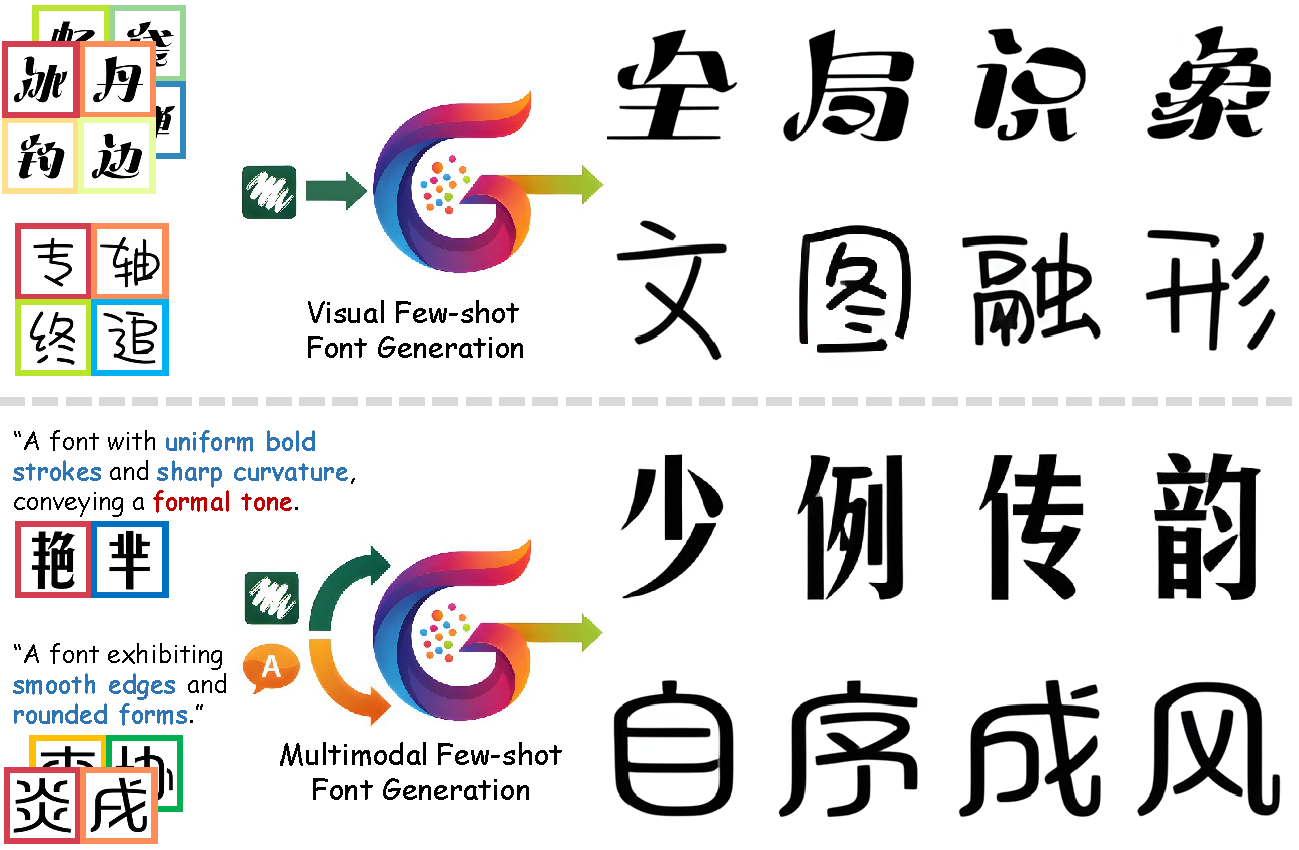
\includegraphics[width=\linewidth]{IMGS/Teaser.pdf}
    \vspace{-3mm}
    \caption{GAR-Font results under visual and multimodal few-shot settings. The generated poem reflects the key contributions of our model: global-aware tokenization for style fidelity, multimodal style encoding for text-image control, reduced reference requirements, and an autoregressive design that enables controllable high-quality font synthesis.}
    \label{fig: Teaser}
    \vspace{-3mm}
\end{figure}
\section{Introduction}

High-quality fonts are central to visual communication, yet their manual creation is costly: practitioners must translate their design concepts into a full, consistent glyph set. This challenge is compounded for logographic systems like Chinese and Japanese, which contain tens of thousands of characters and complex stroke geometries.

Few-shot Font Generation (FFG) seeks to automate this process by generating an entire font library from only a handful of reference examples. However, it presents several technical difficulties. First, it demands precise structural fidelity, where strokes, radicals, and local geometry must be correct for every glyph. Second, it requires capturing a holistic and faithful style representation, generalizing from a handful of examples across diverse characters.

A core obstacle for FFG is the lack of an effective visual global representation. GAN-based methods~\cite{LF_Font, CG_GAN} often exhibit noticeable style discrepancies from the reference fonts, and struggle with stroke-level accuracy. Diffusion models~\cite{Diff_Font, Font_Diffuser, HFH_Font} improve structural correctness and local fidelity but do not guarantee a coherent global style. Existing sequence approaches such as VQ-Font~\cite{VQ_Font} and IF-Font~\cite{IF_Font} rely on local patch or block tokenization, which fragments global cues and leads to noticeable discrepancies from the reference styles. Recent autoregressive (AR) image generation methods~\cite{Titok, SpectralAR} further reveal the superiority of globally contextualized 1D tokens over 2D patched tokenization, highlighting a promising direction for modeling global stylistic patterns in font synthesis. 


Meanwhile, existing FFG frameworks remain single-modal, using only visual modality to control font style. In contrast, linguistic descriptions convey global, conceptual design intents that go beyond visual appearance. They provide complementary representations, helping overcome the limitations of vision-only models when style must be inferred from a few examples.


These insights motivate GAR-Font, an expressive and controllable FFG framework that integrates visual and linguistic information. Leveraging the AR modeling capacity, GAR-Font introduces three major technical contributions:

\begin{itemize}
\item We propose \textbf{a global-aware tokenizer (G-Tok)} that fuses local features with global perception, capturing both fine-grained stroke details and font-level style patterns.
\item We design \textbf{an AR generator with multimodal style encoder}, first pretrained on visual inputs, and then augmented with a lightweight language-style adapter.
\item We introduce \textbf{a post-refinement pipeline} to the font generation process, which improves structural fidelity and stylistic coherence, producing high-quality glyphs from limited references.
\end{itemize}

To validate the effectiveness of GAR-Font, we conduct extensive experiments across multiple settings. In the standard vision-only scenario, it surpasses other competitive FFG methods, demonstrating superior structural and stylistic fidelity. In the multimodal setting, the augmented multimodal style encoder further improves generation quality. Using 4 reference images plus one textual description, GAR-Font matches the quantitative performance of 8 images while providing flexible control. Ablation studies further confirm that G-Tok produces stable and coherent representations that preserve holistic structure and reference style fidelity—key factors for high-quality font synthesis. GAR-Font moves beyond patch-level modeling by learning global-aware representations and enabling text-driven multimodal FFG, establishing a new AR-based solution for automatic and controllable font generation.

% To validate the superiority of GAR-Font, we conduct comprehensive experiments. We compare our method with existing cutting-edge FFG methods in the conventional vision-only scenario, showing its competitive performance. The proposed lightweight language-style adapter further enhances GAR-Font by enabling flexible text-guided style control, improving generation quality while reducing reliance on style references. Moreover, extensive analyses verify the strong global-aware representation capability of the G-Tok, highlighting its ability to preserve holistic structure and coherent style which are key factors for achieving consistent and high-fidelity font synthesis.
\section{Related Work}
\subsection{Autoregressive Image Generation}
Autoregressive (AR) models have shown powerful generation ability across modalities~\cite{Flamingo, Videollava, llavamed, Unifiedio2}, and their extension to visual generation~\cite{ImageTransformer, llamagen, Chameleon, Emu, Emu3, januspro, simpleAR} has demonstrated promising potential. Typically, they follow a two-stage paradigm: a tokenizer encodes images into discrete representations (e.g., VQ-VAEs~\cite{VQ_VAE, VQ_VAE2}, RQ-VAE~\cite{RQ_VAE_RQ_FORMER}, VQ-GAN~\cite{VQ_GAN, VIT_VQGAN}), and a transformer decoder~\cite{MaskGIT, star_scale_wise, VAR, RAR, SpectralAR} that sequentially predicts these tokens for image reconstruction.

Most AR models use 2D patch-wise tokenization, capturing local details but lacking holistic awareness~\cite{MVTQ, EfficientVQGAN, ARPG_LocalTokens, ImageGPT}. To improve global coherence, recent works explore complementary strategies: global-context modeling~\cite{Hita} introduces holistic queries for structural reasoning; frequency-domain methods~\cite{SpectralAR, NFIG} encode coarse-to-fine spectral context; 1D tokenizers~\cite{Titok, FlexTok, InstellaT2I} enhance efficiency but lose adaptability; semantic tokenization~\cite{ImageFolder, TexTok} leverages language priors for meaningful visual codes. Structured visual like glyphs, however, demands tokenizers that unify local stroke detail with global aesthetics. Our GAR-Font addresses this challenge through a \textbf{global-aware tokenizer} that integrates CNN-based locality with Transformer-based global reasoning, effectively unifying fine-grained stroke detail and overall stylistic coherence.

\subsection{Few-shot Font Generation}
Few-shot Font Generation (FFG) can be broadly divided into vector-based and image-based approaches. Vector FFG methods have progressed in sequential modeling and efficient representations~\cite{FontRNN, Deepvecfont, DeepVecFontV2, DualVector, Vecfusion, Vecfontsdf}. Yet complex ideographic generation and unseen glyph generalization remain challenging~\cite{EasyFont, CVFont}. Image-based methods, in contrast, learn 2D pixel priors for robust adaptation, evolving from early image-to-image translation~\cite{zi2zi, word2word, zigan, HGAN} to more recent VQ and diffusion formulations~\cite{Font_Diffuser, HFH_Font, FSTDIFF, VQ_Font}. These models typically employ content–style disentanglement to separately capture structure and style~\cite{zhang2018separating, EMD, AGIS-Net, DG_Font, MX_Font, DS-Font, FineGrainedFFG, fewshotFFG, Xmpfont, Diff_Font}, enhanced by mechanisms like contrastive learning for global coherence~\cite{SCFont} and cross-attention for local transfer~\cite{Fs_Font}.  

The challenge is most acute for glyph-rich, ideographic languages such as Chinese and Korean, where thousands of characters demand fine structure and faithful global style~\cite{LegacyLearning, SCFont, GenerateExpert, HFH_Font}. In this regime, \textbf{image-based AR models that operate FFG on globally contextualized visual tokens} show particular promise: by modeling spatial dependencies directly in the 2D domain, they better capture the intricate geometry and visual regularities of glyphs.

\begin{figure}[t!]
    \centering
    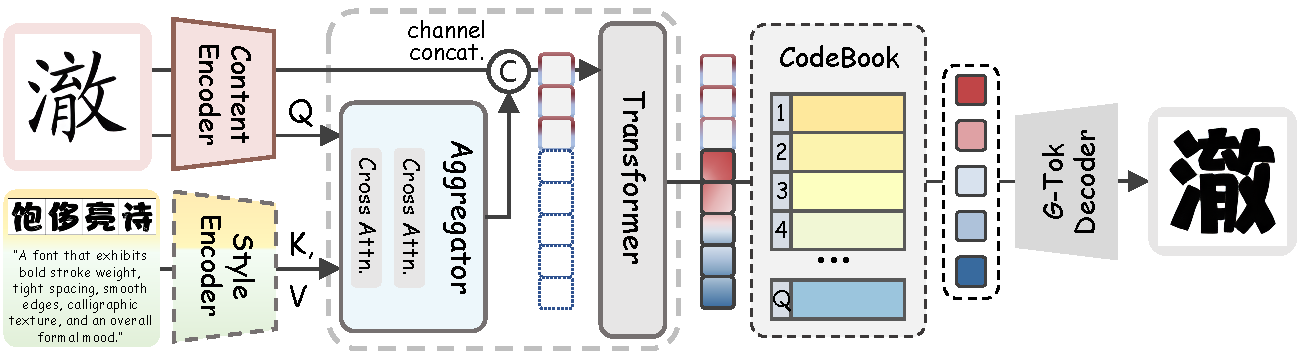
\includegraphics[width=\linewidth]{IMGS/Fig1_Model.pdf}
    \vspace{-4mm}
    \caption{The overall architecture of GAR-Font. It comprises a global-aware tokenizer (G-Tok), and an AR generator, equipped with a multimodal style encoder.}
    \vspace{-3mm}
    \label{fig: Model}
\end{figure}
\begin{figure*}[!t]
\centering
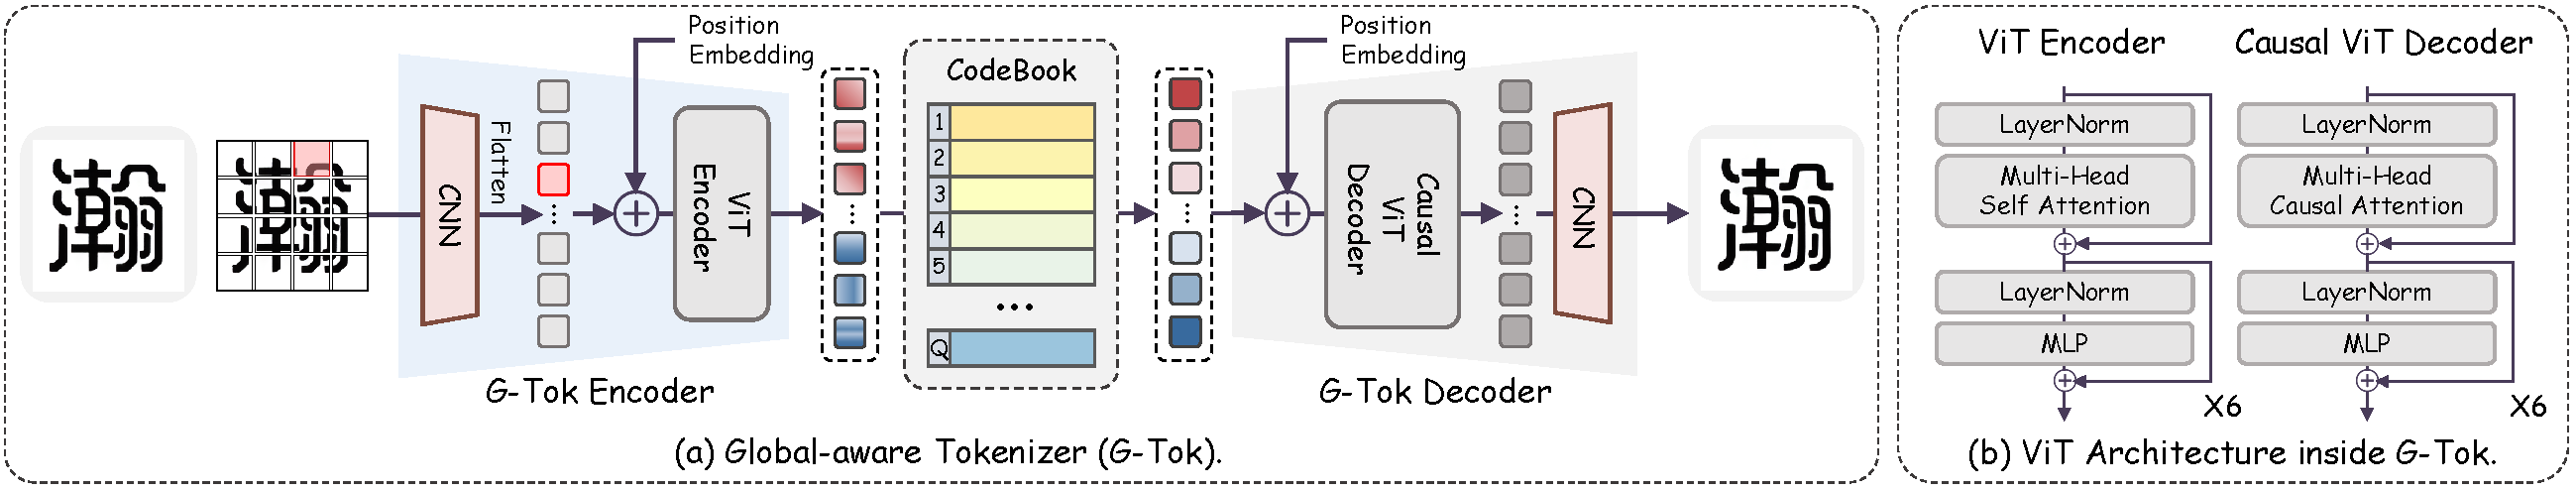
\includegraphics[width=0.99\linewidth]{IMGS/Fig2_G-Tok.pdf}
\vspace{-3mm}
\caption{(a) Overview of the G-Tok architecture, which adopts a hybrid CNN–ViT design. (b) Details of the global ViT encoder and causal ViT decoder. With self- and causal-attention, G-Tok captures global dependencies, enabling coherent and high-quality font synthesis.}
\vspace{-3mm}
\label{fig: G-tok}
\end{figure*}
\subsection{Multimodal Alignment for Style Control}
Multimodal alignment for style control unifies visual and textual modalities for coherent, fine-grained style manipulation. Foundational models~\cite{Emu3, januspro, BAGEL, Seed-X, Qwen-Image, Hunyuan-Image} achieve this through costly multimodal pretraining. For fonts, however, only textual inputs describing style are incorporated, and the independent encoding of content and style in FFG frameworks~\cite{VQ_Font, Fs_Font, LF_Font} naturally forms a structured visual style space that serves as a strong prior for multimodal integration. Recent works pursue efficient alignment via parameter-efficient modules~\cite{FonTS, FontAdapter, LoRA, AdaCLIP} or resampler-based strategies aligning vision and language spaces~\cite{Flamingo, PaLM2-VAdapter, CalliReader, TextAdapter}. Motivated by these works, GAR-Font extends the style encoder in FFG models to a \textbf{multimodal style encoder} that consists of a visual style encoder and a lightweight pluggable \textbf{language-style adapter} that aligns textual descriptions with visual style embeddings, enabling fine-grained, flexible style control without the need for large-scale multimodal pretraining.

\section{Method}
The architecture of GAR-Font is illustrated in Figure~\ref{fig: Model}. Our framework comprises three core components:

\noindent\textbf{A global-aware tokenizer (G-Tok)} discretizes glyphs into tokens, capturing intricate structure and global visual style.

\noindent\textbf{An AR generator with multimodal style encoder} first learns from visual inputs to establish a stable style space, and then employs a lightweight language-style adapter for multimodal style control.

\noindent\textbf{A post-refinement} enhances structural fidelity and style coherence for high-quality few-shot font generation.

Given a content glyph, a few style references, and optional text, GAR-Font encodes and aggregates content and style, autoregressively generates codebook representations and decodes them softly into high-quality glyphs, which are subsequently improved by a post-refining stage. The details of each module adopted in the proposed GAR-Font will be presented in the following subsections.

\subsection{Global-aware Tokenizer}
The Global-aware Tokenizer (G-Tok), shown in Figure~\ref{fig: G-tok}, encodes glyphs into tokens using a hybrid CNN–ViT encoder, a vector quantizer, and a causal hybrid decoder. By fusing local convolutional features with Transformer-based global context, it captures fine-grained structure and overall style, enabling coherent, high-quality font synthesis.

\vspace{-3mm}
\paragraph{Hybrid encoding.} Given a glyph image $\mathbf{I} \in \mathbb{R}^{H \times W \times 3}$, a CNN encoder $E_{\text{CNN}}$ extracts local stroke features, which are flattened and aggregated through a ViT encoder $E_{\text{ViT}}$:
\begin{equation}
    \mathbf{T} = E_{\text{ViT}}\big(\mathrm{Proj}(E_{\text{CNN}}(\mathbf{I})) + \mathbf{P}_{\text{2D}}\big) \in \mathbb{R}^{N\times d},
\end{equation}
where $\mathbf{P}_{\text{2D}}$ refers to the 2D sinusoidal position embeddings~\cite{ViT}, $N$ and $d$ denote token count and embedding dimension. The convolutional backbone preserves spatial locality, capturing fine stroke geometry, while the ViT’s self-attention aggregates tokens globally to enforce style fidelity. This hybrid design captures both structure fidelity and long-range style dependencies.
\vspace{-4mm}
\paragraph{Vector Quantization.} Following standard VQ-VAE~\cite{VQ_VAE} and VQ-GAN~\cite{VQ_GAN}, we discretize latent tokens by mapping them to the nearest entries in a learnable table. We apply the commitment and embedding regularization with an entropy term to stabilize training and preserve diversity.
\vspace{-4mm}
\paragraph{Causal decoding and optimization.} A causal ViT–CNN decoder reconstructs glyph $\hat{\mathbf{I}}$ from quantized tokens, modeling sequential dependencies while convolutional layers refine local details. Figure~\ref{fig: G-tok}(b) illustrates this structure.

The tokenizer is optimized end-to-end with a weighted combination of reconstruction, perceptual, and vector quantization losses:
\begin{equation}
    \mathcal{L}_{\text{tok}} =
\lambda_{\text{rec}}\mathcal{L}_{\text{rec}} +
\lambda_{\text{per}}\mathcal{L}_{\text{per}} +
\lambda_{\text{vq}}\mathcal{L}_{\text{vq}},
\end{equation}
where $\mathcal{L}_{\text{rec}}=\|\mathbf{I}-\hat{\mathbf{I}}\|_1$ denotes the L1 reconstruction loss, $\mathcal{L}_{\text{per}}=\|\Phi(\mathbf{I})-\Phi(\hat{\mathbf{I}})\|_2^2$ represents the perceptual loss, and $\mathcal{L}_{\text{vq}}$ is the standard vector quantization loss. 

\subsection{AR Generator with Multimodal Style Encoder}
Using G-Tok’s global representations, the AR generator performs conditional sequential prediction. To leverage prior FFG insights (Content-style Aggregator) while avoiding the cost of joint image–text training, GAR-Font adopts a decoupled learning paradigm. The generator, aggregator, and style encoder are first trained on visual inputs to learn a stable representation. Based on this foundation, the visual style encoder is extended into a multimodal one through a lightweight, plug-in language adapter that aligns textual cues with learned visual styles, enabling flexible text-guided generation without disturbing the visual prior.

\subsubsection{Pretraining on Visual Modality}
Visualized in Figure~\ref{fig: Training}(a), to build a stable style–content representation, the AR generator is first trained on visual conditions, following the successful practices of prior FFG methods. This ensures robust modeling of both content structure and stylistic variations across glyphs, providing a solid foundation for subsequent multimodal adaptation.
\vspace{-4mm}
\paragraph{Encoders and Content–style Aggregator.} 
As shown in Figure~\ref{fig: Training}(a), we adopt both CNN architectures on the content encoder and the visual style encoder. The Content-style Aggregator follows the previous design~\cite{Fs_Font, LF_Font}. Given a content glyph and $N_s$ style references, the encoders respectively extract content features $\mathbf{F}_c$ and style features$\{\mathbf{F}_{vis_j}\}^{N_s}_{j=1}$. These features are then fused where content queries attend to fine-grained style cues:
\begin{equation}
\tilde{\mathbf{T}}_{\text{vis}} = \mathrm{Aggregator}\big(\mathbf{F}_c, \{\mathbf{F}_{\text{vis}_j}\}_{j=1}^{N_s}\big).
\end{equation}
The aggregated visual representation $\tilde{\mathbf{T}}_{\text{vis}}$ is concatenated with $\mathbf{F}_c$ to form the conditioning input $\mathbf{T}$.
\vspace{-3mm}
\paragraph{Autoregressive modeling and soft decoding.} Conditioned on $\mathbf{T}$, the Transformer-based generator autoregressively predicts the next token at each timestep, producing logits $\mathbf{L}$ over the codebook $\mathcal{C}$ of G-Tok. Instead of standard discrete hard decoding, we employ a soft projection that maps $\mathbf{L}$ onto the codebook 
$\tilde{\mathbf{Z}} = \mathrm{Softmax}(\mathbf{L}) \cdot \mathcal{C}$.
This continuous mapping not only preserves gradient flow during training, enabling pixel-level supervision, but can also be applied at inference. Using soft projection at inference improves stroke continuity and glyph fidelity by leveraging the full expressive capacity of the codebook, yielding smoother and more accurate glyphs compared with discrete hard decoding.
\vspace{-3mm}
\paragraph{Training objectives.} During this visual-pretraining stage, the aggregator, generator, and style encoder are jointly optimized with a combined token and pixel-level loss:
\begin{equation}
\mathcal{L}_{\text{AR}} = \lambda_{\text{CE}}\mathcal{L}_{\text{CE}} + \lambda_{\text{pixel}}\mathcal{L}_{\text{pixel}},
\end{equation}
where $\mathcal{L}_{\text{CE}}$ is the cross-entropy loss over the target token indices $\mathbf{s}$, and $\mathcal{L}_{\text{pixel}}$ measures the L1 reconstruction error between the generated glyph $\hat{\mathbf{I}}_f$ and ground truth $\mathbf{I}_f$. 

\subsubsection{Multimodal Style Encoder Adaptation}
Visual pretraining forms a stable style–content space but lacks high-level conceptual control. To address this, we introduce a lightweight, plug-in language adapter that aligns textual design cues with visual style representations, as shown in Figure~\ref{fig: Training}(b). Through this adapter, the style encoder is extended into a multimodal form, enabling flexible text-guided modulation without disrupting the visual prior.
\vspace{-3mm}
\paragraph{Vision-language Adapter.} The adapter bridges textual descriptions and visual style features through an iterative cross-attention mechanism. Specifically, a subset of visual style features $\{\mathbf{F}_{vis_j}\}^{k}_{j=1}$ is first extracted from $k<N_s$ reference glyphs by the visual style encoder, while a textual font description embedding is derived from a pretrained Flan-T5 encoder. The text embedding is projected into the visual feature space and iteratively refined by attending to the given style features. The aligned textual–visual token is then spatially expanded into $\mathbf{F}_t$ and concatenated with the visual features:
\begin{equation}
\tilde{\mathbf{F}}_{mm} = [\mathbf{F}_{vis_1}, \ldots, \mathbf{F}_{vis_k}, \mathbf{F}_t].
\end{equation}
\paragraph{Training objectives.} 
The multimodal style encoder may produce features $\tilde{\mathbf{F}}_{mm}$ with token lengths different from those of the visual-only encoder, due to variations in the number of visual references. Thus, we supervise training on their aggregated objectives. Specifically, $\tilde{\mathbf{T}}_{\text{mm}}$ and $\tilde{\mathbf{T}}_{\text{vis}}$ are obtained by aggregating $k$ visual plus one textual reference, and all $N_s$ visual references, respectively. We train the adapter by minimizing the $\ell_2$ distance between these two aggregated representations:
\begin{equation}
\mathcal{L}_{\text{adapt}} = \|\tilde{\mathbf{T}}_{\text{mm}} - \tilde{\mathbf{T}}_{\text{vis}}\|_{2}^{2}.
\end{equation}
\vspace{-1mm}
This objective encourages the multimodal encoder to internalize stylistic intent consistent with the full-visual setting, facilitating effective text–style substitution and reducing reliance on visual inputs.
\begin{figure}[t!]
    \centering
    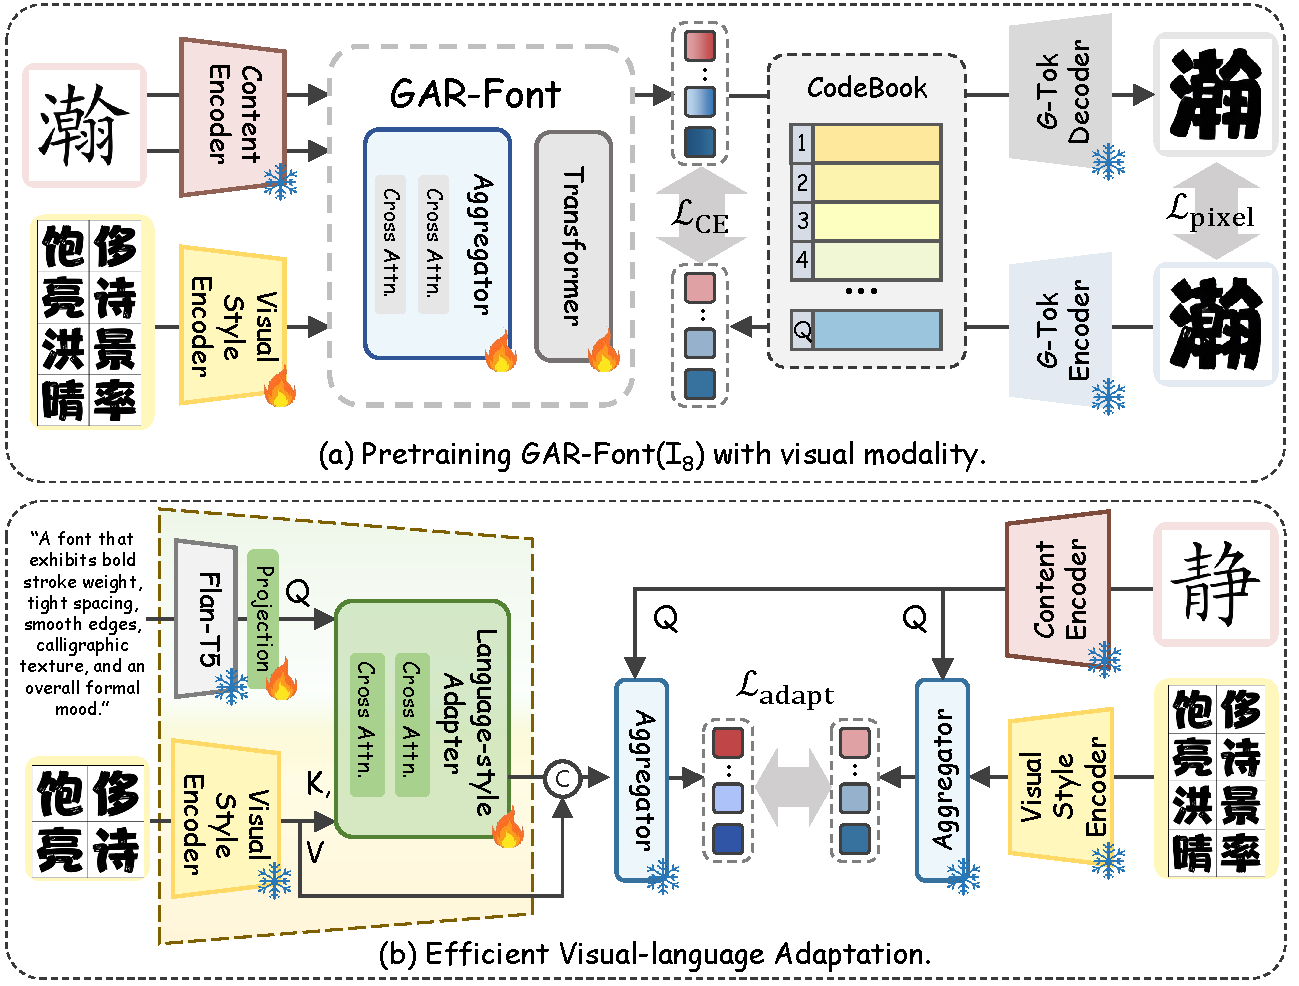
\includegraphics[width=\linewidth]{IMGS/Fig3_Train.pdf}
    \vspace{-5mm}
    \caption{GAR-Font adopts a two-stage training: (a) Visual Pretraining builds a stable content–style space via token and pixel losses; (b) Vision–language Adaptation aligns text embeddings with style features with a lightweight adapter for text-guided generation while preserving visual priors.}
    \label{fig: Training}
    \vspace{-5mm}
\end{figure}
\vspace{-1mm}
\subsection{Post-refinement}
GAR-Font adopts a two-stage post-refinement to improve few-shot style generalization and structural accuracy: novel font adaptation (NFA) and structural enhancement (SE).
\vspace{-3mm}
\paragraph{Novel font adaptation (NFA) for few-shot generalization.} The pretrained generator learns general font patterns but fails to model unseen styles precisely. NFA mitigates this by performing a lightweight adaptation using a few reference glyphs, updating the LoRA layers of the Transformer generator with a mixed token–pixel loss:
\begin{equation}
\mathcal{L}_{\text{SFT}}=\lambda_{\text{CE}}\mathcal{L}_{\text{CE}}+\lambda_{\text{pixel}}\mathcal{L}_{\text{pixel}},
\end{equation}
where $\mathcal{L}_{\text{CE}}$ is the token cross-entropy and $\mathcal{L}_{\text{pixel}}=|\hat{\mathbf{I}}-\mathbf{I}|_1$ encourages pixel-level accuracy. This yields stable few-shot adaptation and better preservation of unseen styles.
\vspace{-3mm}
\paragraph{Structural enhancement (SE) for precise glyph reconstruction.}
While NFA enhances style fidelity, minor structural distortions may remain. To enhance structural clarity and readability, SE further refines glyphs using a group-relative optimization based on GRPO~\cite{DeepseekMath_GRPO}. The generator is treated as a policy $\pi_\theta$ that outputs token sequences $\mathbf{s}$; each decoded glyph receives a composite reward:
\begin{equation}
r=\lambda_{\text{ocr}}\,r_{\text{ocr}}+\lambda_{\text{style}}\,r_{\text{style}},
\end{equation}
\vspace{-1mm}
where $r_{\text{ocr}}$ is obtained from a pretrained OCR model as
\vspace{-2mm}
\begin{equation}
r_{\text{ocr}}=
\begin{cases}
p_{\text{ocr}}, & \text{if } \hat{y}=y,\\[3pt]
0, & \text{otherwise.}
\end{cases}
\end{equation}

Here $p_{\text{ocr}}$ is recognition confidence, and $r_{\text{style}}$ measures consistency with the reference style using a pretrained style discriminator.

%with $p_{\text{ocr}}$ denoting the recognition confidence and $y$ the ground-truth label. $r_{\text{style}}$ evaluates stylistic consistency with reference fonts and mitigates style degradation using a pretrained style discriminator.

Rewards are normalized within each sampled group to compute advantages $A^{(k)} = \frac{r^{(k)} - \mu(r)}{\sigma(r)}$. SE updates only the LoRA layers by maximizing advantage-weighted likelihood with KL regularization to a frozen reference policy:
\vspace{-1mm}
\begin{equation}
\mathcal{L}_{\text{SE}} \!=\! -\mathbb{E}_{\mathbf{s}\sim\pi_\theta}\big[A(\mathbf{s})\log\pi_\theta(\mathbf{s})\big]+\beta\,\mathrm{KL}(\pi_\theta\|\pi_{\text{ref}}),
\end{equation}
where $A(\mathbf{s})$ denotes the group-normalized advantage and $\pi_{\text{ref}}$ is the frozen reference policy used for stability.  

% % The architecture of GAR-Font is illustrated in Figure~\ref{}.
% % Our training pipeline comprises three stages.
% % First, a Global-aware Tokenizer based on a hybrid CNN–ViT design discretizes glyphs into compact tokens that encode both local stroke details and global stylistic dependencies.
% % Second, an Autoregressive Generator conditioned on content and style references models target glyph tokens via a Transformer decoder, ensuring structural integrity and stylistic coherence.
% % Finally, a Post-Training Refinement stage combining supervised fine-tuning and GRPO-based reinforcement learning further enhances generalization and structural fidelity.
% % This unified design enables multimodal, text-driven, few-shot font generation with consistent global style. \lyx{SHOULD MODIFY DEPENDS ON THE VISUALIZATION! NOW WE DON'T HAVE A THREE-STAGE VISUAL!!!!!!}

% The architecture of GAR-Font is illustrated in Figrue ~\ref{}.
% Our framework comprises two sequential training stages and one auxiliary module for multimodal guidance. 

% In the pre-training stage, a global-aware tokenizer is trained to discretize glyphs into compact visual tokens, which are then modeled by an autoregressive generator to reconstruct target glyphs with coherent structure and style.

% On top of the pretrained generator, a lightweight language-style adapter injects textual stylistic cues into the visual embedding space, enabling multimodal control and improving generation quality under limited reference conditions.

% Finally, the post-training stage combines supervised fine-tuning and GRPO-based reinforcement learning to further improve structural fidelity and generalization on novel fonts.


% \subsection{Global-aware Tokenizer}

% The Global-Aware Tokenizer (G-Tok) discretizes glyphs into compact tokens encoding both structural and stylistic information. It consists of a hybrid CNN–ViT encoder, a vector quantizer, and a causal hybrid decoder.
% \begin{figure*}
% \centering
% \includegraphics[width=1.0\linewidth]{TEMP_IMGS/TEMP_G_Tok.jpg}
% \end{figure*}

% \paragraph{Hybrid encoding.} Given a glyph image $\mathbf{I} \in \mathbb{R}^{H \times W \times 3}$, a CNN encoder $E_{\text{CNN}}$ extracts local stroke features, which are flattened and aggregated through a ViT encoder $E_{\text{ViT}}$:
% \begin{equation}
%     \mathbf{T} = E_{\text{ViT}}\big(\mathrm{Proj}(E_{\text{CNN}}(\mathbf{I})) + \mathbf{P}_{\text{2D}}\big) \in \mathbb{R}^{N\times d},
% \end{equation}
% where $\mathbf{P}_{\text{2D}}$ denotes 2D sinusoidal positional embeddings~\cite{ViT}, $N$ and $d$ denote token count and embedding dimension. The convolutional backbone ensures strong spatial locality, critical for capturing the fine-grained stroke geometry. At the same time, multi-head self-attention in the ViT encoder enhances global style consistency by aggregating token information across all spatial positions. This hybrid design captures both structure fidelity and long-range style dependencies crucial for font synthesis.

% \paragraph{Vector Quantization.} We adopt a standard vector quantization scheme following VQ-VAE~\cite{VQ_VAE} and VQ-GAN~\cite{VQ_GAN}, where latent tokens are discretized by mapping to the nearest entries in a learnable codebook. To stabilize codebook usage and preserve representational diversity, we employ commitment and embedding regularization with an additional entropy term. The resulting discrete sequence serves as the autoregressive modeling target.

% \paragraph{Causal decoding and optimization.} A causal ViT-CNN decoder reconstructs glyphs from quantized tokens, integrating global self-attention with local convolutional refinement. 
% The tokenizer is optimized end-to-end with a weighted combination of reconstruction, perceptual, and vector quantization losses:
% \begin{equation}
%     \mathcal{L}_{\text{tok}} =
% \lambda_{\text{rec}}\mathcal{L}_{\text{rec}} +
% \lambda_{\text{per}}\mathcal{L}_{\text{per}} +
% \lambda_{\text{vq}}\mathcal{L}_{\text{vq}},
% \end{equation}
% where $\mathcal{L}_{\text{rec}}=\|\mathbf{I}-\hat{\mathbf{I}}\|_1$ denotes the L1 reconstruction loss, $\mathcal{L}_{\text{per}}=\|\Phi(\mathbf{I})-\Phi(\hat{\mathbf{I}})\|_2^2$ represents the perceptual loss, and $\mathcal{L}_{\text{vq}}$ is the standard vector quantization loss. 
% This training yields discrete representations that preserve both structural fidelity and global stylistic coherence for downstream autoregressive generation.
% \lyx{PLEASE DESIGNATE ALL THE EQUATIONS, WHETHER THEY ARE WRITTEN CORRECTLY AND WHETHER THEY HAVE ALL THE COMPONENTS WELL-DEFINED (e.g, where A denotes xxx, B denotes xxx,  etc.). PLEASE BE SURE ALL THE COMPONENTS ARE DEFINED!!!!}



% \subsection{Autoregressive Generator}
% The autoregressive generator produces target glyphs that preserve the structural layout of a content glyph $\mathbf{I}_c$ while adopting styles from $N_s$ reference glyphs $\{\mathbf{I}_{s_j}\}_{j=1}^{N_s}$. The generation pipeline consists of three stages: content–style encoding and fusion, autoregressive token prediction, and image reconstruction from predicted tokens (Fig.~\ref{}).

% \begin{figure}[t]
%   \centering
%   %\fbox{\rule{0pt}{2in} \rule{0.9\linewidth}{0pt}}
%   \includegraphics[width=1.0\linewidth]{TEMP_IMGS/TEMP_Generator_2.jpg}

%    \caption{EXAMPLE2 : Architecture of GAR-Font}
%    \label{fig:onecol}
% \end{figure}

% \paragraph{Content-style encoding and fusion.} A content encoder $E_c$ and a style encoder $E_s$ extract features from the content and style glyphs, respectively. Iterative cross-attention blocks~\cite{Fs_Font, VQ_Font} inject fine-grained style information into content features, and the resulting style-enhanced features are concatenated with the content features to form the final conditioning representation $\mathbf{T}_{\text{cond}}$ (as illustrated in Figure~\ref{}).

% \paragraph{Autoregressive token generation.} The Transformer-based autoregressive generator takes $\mathbf{T}_{cond}$ as context and models the sequential dependencies within the discrete token sequence $\mathbf{s}$ generated by G-Tok. Predicted logits $\mathbf{L}$ are softly projected onto the codebook $\mathcal{C}$ as $\tilde{\mathbf{Z}}=\mathrm{Softmax}(\mathbf{L})\mathcal{C}$, producing continuous embeddings that are decoded by the G-Tok decoder $D$ to reconstruct the glyph image $\hat{\mathbf{I}}_f$. This differentiable decoding maintains gradient flow and enables smoother transitions in the latent space, bridging the gap between discrete token prediction and continuous image reconstruction to enhance visual quality.

% \paragraph{Training objectives.} The generator is optimized with a combined token and pixel-level loss:

% \begin{equation}
% \mathcal{L}_{\text{total}} = \lambda_{\text{CE}}\mathcal{L}_{\text{CE}} + \lambda_{\text{pixel}}\mathcal{L}_{\text{pixel}},
% \end{equation}
% where $\mathcal{L}_{\text{CE}}$ is the cross-entropy loss over the target token indices $\mathbf{s}$, and $\mathcal{L}_{\text{pixel}}$ measures L1 reconstruction error between the generated glyph $\hat{\mathbf{I}}_f$ and ground truth $\mathbf{I}_f$. This compact objective enforces accurate sequential modeling and high-fidelity glyph reconstruction.
% \lyx{YOU MAY ADD MORE DETAILS, AND ALSO THE DETAILS OF MULTIMODALITY!!!!!!}



% \subsection{Lightweight Language-Style Adapter}
% To enhance few-shot generation under more limited reference conditions, we propose a lightweight language-style adapter that injects textual stylistic guidance into the pretrained autoregressive generator without additional multimodal pretraining. The adapter establishes a shared representation space between textual font descriptions and visual style embeddings, enabling flexible multimodal control.

% \paragraph{Language–style feature alignment.}
% Given a subset of visual style features ${\mathbf{F}_{s_j}},{j=1,2,..,k}$ extracted from $k<N_s$ style reference glyphs  through the style encoder $E_s$ and a textual font description embedding $\mathbf{E}_t$ obtained from a pretrained T5 encoder, the adapter aligns these modalities through iterative cross-attention interactions.
% Specifically, the text embedding $\mathbf{E}_t$ is first projected into the visual feature space and then refined by attending to stylistic visual features ${\mathbf{F}_{s_j}},{j=1,2,..,k}$, allowing the text representation to absorb fine-grained visual attributes from limited references. This process effectively injects stylistic semantics into the textual embedding while maintaining its global descriptive coherence.

% \paragraph{Language-style Fusion and pseudo-style representation.}
% After alignment, the aggregated textual-visual token is expanded spatially and concatenated with the remaining visual style features to form a unified pseudo-style representation:
% \begin{equation}
% \tilde{\mathbf{F}}_s = [\mathbf{F}_{s_1}, \ldots, \mathbf{F}_{s_k}, \mathbf{F}_t],
% \end{equation}
% where $\mathbf{F}_t$ denotes the text-fused representations. This fused style representation is then integrated with the content encoding through the generator’s feature fusion module, serving as a multimodal conditioning input for subsequent autoregressive generation.

% \paragraph{Training objectives.}
% The adapter is optimized under a teacher–student framework, where a pretrained generator serves as the teacher to provide full style fusion supervision. The teacher produces complete fused feature representations using all available style references, while the student—equipped with the proposed adapter—predicts pseudo-style representations from fewer visual references and corresponding textual descriptions.
% By minimizing the discrepancy between teacher and student fused representations, the adapter learns to recover missing stylistic cues from linguistic guidance and to generalize across unseen font styles.
% The overall training objective is defined as:
% \begin{equation}
% \mathcal{L}_{\text{adapter}} = \|\tilde{\mathbf{F}}_{s}^{\text{student}} - \tilde{\mathbf{F}}_{s}^{\text{teacher}}\|_{2}^{2},
% \end{equation}
% where $\tilde{\mathbf{F}}_{s}^{\text{teacher}}$ and $\tilde{\mathbf{F}}_{s}^{\text{student}}$ denote the fully fused and pseudo-style fused feature representations, respectively.

% This feature-level reconstruction loss enforces consistent multimodal alignment and encourages the adapter to infer complementary visual information from textual style descriptions and limited references.


% \subsection{}

% \subsection{Post-training}
% To improve stylistic fidelity and glyph structure, GAR-Font applies a two-stage post-training: supervised fine-tuning (SFT) for few-shot adaptation and reinforcement learning (RL) for structural refinement.

% \paragraph{Supervised fine-tuning (SFT) for novel font adaptation.}
% While the pretrained generator captures overall font styles, it still tends to overfit seen styles when adapting to unseen ones, reducing style fidelity. To mitigate this, GAR-Font applies a supervised fine-tuning (SFT) stage for targeted adaptation using a few reference glyphs. 
% SFT updates a small subset of parameters (style encoder, fusion module, and LoRA layers) and optimizes a combined token–pixel objective:
% \begin{equation}
% \mathcal{L}_{\text{SFT}}=\lambda_{\text{CE}}\mathcal{L}_{\text{CE}}+\lambda_{\text{pixel}}\mathcal{L}_{\text{pixel}},
% \end{equation}
% where $\mathcal{L}_{\text{CE}}$ denotes the cross-entropy over target token indices and $\mathcal{L}_{\text{pixel}}=\|\hat{\mathbf{I}}-\mathbf{I}_{\text{tar}}\|_1$ measures L1 reconstruction between the decoded glyph $\hat{\mathbf{I}}$ and ground truth $\mathbf{I}_{\text{tar}}$. 
% This lightweight SFT ensures stable few-shot adaptation, enabling faithful preservation of unseen styles while maintaining content consistency.

% \paragraph{Reinforcement learning for glyph structural refinement.}
% While SFT improves style fidelity, generated glyphs may still exhibit subtle structural distortions. To enhance structural clarity and readability, we introduce a reinforcement learning (RL) stage built upon the Group Relative Policy Optimization (GRPO) framework~\cite{DeepseekMath_GRPO}. The generator is fine-tuned as a policy $\pi_\theta$ that produces token sequences $\mathbf{s}$ conditioned on $\mathbf{T}_{cond}$. Each generated glyph $\hat{\mathbf{I}}$ receives a composite reward:
% \begin{equation}
% r=\lambda_{\text{ocr}}\,r_{\text{ocr}}+\lambda_{\text{style}}\,r_{\text{style}},
% \end{equation}
% where $r_{\text{ocr}}$ is derived from an OCR recognizer as
% \begin{equation}
% r_{\text{ocr}}=
% \begin{cases}
% p_{\text{ocr}}, & \text{if } \hat{y}=y,\\[3pt]
% 0, & \text{otherwise,}
% \end{cases}
% \end{equation}
% with $p_{\text{ocr}}$ denoting the recognition confidence and $y$ the ground-truth label, while $r_{\text{style}}$ measures stylistic consistency to the references and prevents collapse via a pretrained style discriminator.

% We normalize rewards across the sampled group and compute group-relative advantages $A^{(k)} = \frac{r^{(k)} - \mu(r)}{\sigma(r)}$. The policy is updated by maximizing the advantage-weighted log-likelihood with a KL regularizer to a frozen reference policy:
% \begin{equation}
% \mathcal{L}_{\text{GRPO}} \!=\! -\mathbb{E}_{\mathbf{s}\sim\pi_\theta}\big[A(\mathbf{s})\log\pi_\theta(\mathbf{s})\big]+\beta\,\mathrm{KL}(\pi_\theta\|\pi_{\text{ref}}),
% \end{equation}
% where $A(\mathbf{s})$ denotes the group-normalized advantage and $\pi_{\text{ref}}$ is the frozen reference policy used for stability.  
% .


% %\subsection{Global-aware Tokenizer}
% %The global-aware hybrid CNN-ViT tokenizer (G-Tok) constitutes the foundational representation module of GAR-Font, providing discrete, structural and stylistic context-rich representations for autoregressive modeling. As illustrated in <<Fig>>, our tokenizer consists of three major parts : a hybrid CNN-ViT Encoder, Vector Quantizer, and hybrid ViT-CNN Decoder. By combining the spatial sensitivity of convolutions with the global contextual modeling of Transformers, the tokenizer achieves superior extraction of both structural details and holistic stylistic features, which are essential for the FFG task.

% %\subsubsection{Local-Global Hybrid Encoding for Glyph Representation.}
% %Given an input glyph image $\mathbf{I}_f \in \mathbb{R}^{H \times W \times 3}$, the encoder first extracts spatially coherent patch-level features through a series of convolutional blocks:

% %$$\mathbf{F}_{e-cnn} = E_{cnn}(\mathbf{I}_f) \in \mathbb{R}^{C \times h \times w}$$

% %The convolutional backbone ensures strong spatial locality and structural precision, which are critical for capturing the intricate compositional patterns of glyphs.

% %To enhance global perception, $\mathbf{F}_{\text{cnn}}$ is projected into a latent embedding space and flattened into a token sequence for subsequent contextual aggregation:

% %$$\mathbf{T}_{e-cnn} = \mathrm{Flatten}(\mathrm{Proj}(\mathbf{F}_{e-cnn})) \in \mathbb{R}^{N \times d}, \quad N = h \times w$$


% %These tokens are then fed into a Vision Transformer encoder $E_{\text{ViT}}$, equipped with 2D positional embeddings:

% %$$\mathbf{T}_{e-vit} = E_{vit}(\mathbf{T}_{e-cnn} + \mathbf{P}_{2D}) \in \mathbb{R}^{N \times d}, \quad N = h \times w$$

% %Through multi-head self-attention, each token aggregates information across all spatial positions an gains larger receptive fields, enabling the model to capture long-range dependencies and global stylistic coherence.

% %By unifying convolutional local feature extraction capability and transformer-based  global context modeling power, our encoder generates structural precise and globally contextualized representations.


% %\subsubsection{Vector Quantization and Token Discretization.}
% %Folowing the principles of VQ-VAE ~\cite{VQ_VAE} and VQ-GAN ~\cite{VQ_GAN} , the continuous latent embeddings produced by the encoder are discretized into a learnable codebook, denoted as $ C = \{c_{k} \in R^{d}\}^{K}_{k=1}$. 
% %After encoding a glyph image into continuous tokens $\mathbf{T}_{vit} \in \mathbb{R}^{N \times d}$, token-wise quantization $q(\text{·})$ is performed to replace each embedding with its nearest entry in the codebook : 

% %$$\mathbf{Z}_q(i) = q(\mathbf{T}_{e-vit}(i)) := \arg\min_{\mathbf{c}_k \in \mathcal{C}} 
% %\| \mathbf{T}_{e-vit}(i) - \mathbf{c}_k \|_2$$

% %This process yields  a quantized latent representation $Z_{q} \in \mathbb{R}^{N \times d}$ and its corresponding discrete index sequence $s = \{ s_{i}\}^{N}_{i=1}$, which serves as the autoregressive modeling target in subsequent stages.

% %To guide codebook training and encourage diverse codebook usage, we apply the standard vector quantization loss:

% %$$\mathcal{L}_{vq} = \alpha \| sg(T_{e-vit})-Z_{q}\|_{2}^{2}+\beta \| T_{e-vit}-sg(Z_{q})\|_{2}^{2}+\gamma \mathcal{L}_{entropy}$$

% %where $sg(\text{·})$ denotes the stop-gradient operation and $\mathcal{L}_{entropy}$ regularizes codebook utilization entropy to prevent codebook collapse.

% %This discretization process transforms the continuous representation into compact, semantically meaningful discrete tokens, forming the foundation for autoregressive glyph modeling.

% %\subsubsection{Causal Decoding and Reconstruction Objectives.}
% %To reconstruct glyph images from quantized tokens, a causal hybrid ViT-CNN decoder is introduced, mirroring the encoder design while introducing a causal self-attention mechanism. This design models sequential dependencies among tokens, aligned with the autoregressive paradigm of downstream generation process.

% %Given the quantized sequential tokens $\mathbf{Z}_q \in \mathbb{R}^{N \times d}$, 
% %the causal ViT decoder first processes them with 2D positional embeddings:

% %$$ \mathbf{T}_{d-vit} = \text{CausalViT}(\mathbf{Z}_q + \mathbf{P}_{2D}) $$

% %Then, $\mathbf{T}_{d-vit}$ is projected to the latent space and reshaped into a spatial representation:

% %$$ \mathbf{F}_{d-vit} = \text{Reshape}(\text{Proj}(\mathbf{T}_{d-vit})) \in \mathbb{R}^{C \times H \times W} $$

% %which is subsequently decoded by the CNN decoder $D_{cnn}$ to reconstruct the input glyph image:
% %$$ \hat{\mathbf{I}}_f = D_{cnn}(\mathbf{F}_{d-vit}) $$

% %The tokenizer is jointly optimized in an end-to-end manner with a  weighted combination of 
% %reconstruction loss $\mathcal{L}_{rec}$, 
% %perceptual loss $\mathcal{L}_{per}$, 
% %and vector quantization loss $\mathcal{L}_{vq}$:

% %$$ \mathcal{L}_{tokenizer} =\lambda_{rec} \mathcal{L}_{rec} + \lambda_{per}\mathcal{L}_{per} + \lambda_{vq}\mathcal{L}_{vq} $$
% %where $\mathcal{L}_{rec} = \| \mathbf{I}_f - \hat{\mathbf{I}}_f \|_1$ 
% %and $\mathcal{L}_{per} = 
% %\| \Phi(\mathbf{I}_f) - \Phi(\hat{\mathbf{I}}_f) \|_2^2$, 
% %with $\Phi(\cdot)$ denoting a pretrained VGG-based <CITE : VGG ref> perceptual feature extractor.

% %\subsection{Autoregressive Generator}
% %The autoregressive generator synthesizes a target glyph image that preserves the structural layout of a standard content glyph $\mathbf{I}_c \in \mathbb{R}^{H \times W \times 3}$ while maintaining the stylistic patterns from $N_{s}$ style reference glyphs $\{I_{s_{j}}\}^{N_s}_{j=1}$. The process consists of three main stages:(1) content-style encoding with attention-based fusion, (2) autoregressive next-token prediction; and (3) optimization via a weighted combination of token loss and pixel loss. The overall architecture is depicted in <Fig>.

% %\subsubsection{Content–Style Encoding and Fusion.}
% %Following prior FFG works ~\cite{Fs_Font, VQ_Font}, GAR-Font employs a iterative cross-attention mechanism to attentively capture and integrate fine-grained styles. Specifically, a content encoder $E_c$ and a style encoder $E_s$ extract representations $f_{c} \in \mathbb{R}^{hw \times C}$and $f_{s} \in \mathbb{R}^{khw \times C}$ from content glyph $\mathbf{I}_c$ and style glyphs $\{I_{s_{j}}\}^{N_s}_{j=1}$ respectively. A multi-layer Feature Fusion Module (FFM) integrates fine-grained style information through iterative cross-attention:

% %$$ A_{style} = \frac{(W^{Q}f_{c})(W^{K}f_{s})^T}{\sqrt{C}}, f_{cs} = Softmax(A_{style}) \times (W_{V}F_{s})$$

% %where $W^{Q}$, $W^{K}$, $W^{V}$ are learnable parameters to project the extracted features into query and key, and $C$ is the dimension of the key.

% %Stacking $L$ cross-attention blocks progressively results in a completive integration of content and style attributes $F_{fused} \in \mathbb{R}^{hw \times C}$. To maintain structural features, following ~\cite{Fs_Font}, $f_c$ and $F_{fused}$ are concatenated to form the conditioning representation $T_{cond} \in \mathbb{R}^{hw \times 2C}$.

% %\subsubsection{Autoregressive Token Generation.}
% %Conditioned on $T_{cond}$, a Transformer-based autoregressive generator models the sequential dependencies among discrete token indices $ s = \{s_{i}\}_{i=1}^{N}$ corresponding to the quantized embeddings from G-Tok.

% %Formally, the autoregressive model defines a joint distribution over tokens as :

% %$$ P(\mathbf{s} \,|\, \mathbf{T}_{cond}) = \prod_{i=1}^{N} P(s_i \,|\, s_{<i}, \mathbf{T}_{cond})$$

% %This causally sequential formulation aligns with the tokenization stage, modeling the long-range structural dependencies and stylistic coherence.

% %The autoregressively predicted logits $\mathbb{L} $ are softly quantized via the the G-Tok codebook $\mathcal{C}$:
% %$$ \tilde{\mathbf{Z}} = \mathrm{Softmax}(\mathbf{L}) \, \mathcal{C} $$.

% %The resulting continuous embeddings $\tilde{\mathbf{Z}}$ are directly fed into the G-Tok decoder $D$, which integrates global contextual reasoning from the ViT layers and spatial detail restoration form the CNN backbone to reconstruct the target glyph image :

% %$$\hat{\mathbf{I}}_{f} = D(\tilde{\mathbf{Z}})$$


% %This differentiable decoding strategy preserves gradient flow and stabilizes training process, which is critical for high-fidelity font synthesis.

% %\subsubsection{Training Objectives.}
% %The autoregressive generator is optimized with two objectives : a token-level prediction loss and a pixel-level reconstruction loss.

% %The token-level prediction loss enforces accurate sequential modeling by guiding the generator to predict each target token conditioned on preceding tokens and $T_{cond}$. It is formulated as a standard corss-entropy loss over the ground-truth token indices $mathbf{s}$ the predicted logits $\mathbf{L}$ :

% %$$\mathcal{L}_{\text{CE}} = - \frac{1}{N} \sum_{i=1}^{N} \log P(s_i \,|\, s_{<i}, \mathbf{T}_{cond}) $$,

% %where $\mathbf{T}_{cond}$ represents the fused conditioning features and $N$ is the token sequence length.

% %To further enhance the perceptual and structural quality of the reconstructed glyphs, the predicted logits $\mathbf{L}$ are softly quantized via G-Tok codebook $\mathcal{C}$, producing continuous token embeddings that are decoded by G-Tok decoder $D$ to yield the reconstructed glyph $\hat{\mathbf{I}}_f$. The reconstruction loss measures pixel-level fidelity between the generated glyph and the ground truth:
% %$$ \mathcal{L}_{\text{pixel}} = \| \hat{\mathbf{I}}_{f} - \mathbf{I}_{f} \|_1 $$

% %The final training objective combines the two loss : 

% %$$\mathcal{L}_{\text{total}} = \lambda_{\text{CE}} \mathcal{L}_{\text{CE}} + \lambda_{\text{pixel}} \mathcal{L}_{\text{pixel}}.$$



% %\subsection{Post Training}
% %To further refine stylistic features and structural precision, GAR-Font first introduces a post-training stage composed of supervised fine-tuning (SFT) and reinforcement learning (RL). The SFT phase enhances few-shot adaptability and stylistic stability, while the RL phase strengthens structural coherence and readability of generated glyphs.

% %\subsubsection{Supervised Fine-tuning for Novel Fonts Adaptation}
% %Although our pretrained generator effectively captures holistic font style representations, it still faces the same challenge as existing few-shot font generation(FFG) methods when adapting to unseen fonts-tending to approximate novel styles by simply aligning them with a similar seen ones, which compromises style fidelity. To mitigate this bias, GAR-Font performs a supervised fine-tuning (SFT) stage that achieves targeted Adaptation to new fonts with only a few reference glyphs.

% %The procedure follows the same training pipeline as pretraining, while updates only a small set of parameters, including those in the style encoder, feature fusion module, and the LoRA-adapted layers of the autoregressive generator.

% %Given a target glyph image $I_{tar}$, its content glyph $I_c$ and a set of style references $\{I_{s_{j}}\}$, the generator predicts discrete tokens and reconstructs the glyph under two training objectives:

% %$$\mathcal{L}_{CE} = \text{CrossEntropy}(\text{logits}, \text{targets}),\mathcal{L}_{pixel} = \| \hat{\mathbf{I}} - \mathbf{I}_{tar} \|_{1}$$

% %The total supervised fine-tuning loss is:

% %$$ \mathcal{L}_{total} = \lambda_{CE} \mathcal{L}_{CE} + \lambda_{pixel} \mathcal{L}_{pixel}
% % $$

% %This SFT process ensures stable few-shot adpation, enabling GAR-Font to faithfully preserve stylistic cues from unseen fonts while maintaining high content consistency.


% %\subsubsection{Reinforcement learning for glyph structural refinement}
% %While the SFT stage enhances style fidelity for novel fonts, the generated glyphs may still exhibit subtle structural distortions issues. To further refine the glyph quality, we introduce a reinforcement learning (RL) stage built upon the Group Relative Policy Optimization (GRPO) framework ~\cite{DeepseekMath_GRPO}. The generator is regarded as a policy network $\pi_{\theta}$, which models a probability distribution over token sequences conditioned on the content-style fusion representation $T_{cond}$:

% %$$P_{\theta}(\mathbf{s} \,|\, \mathbf{T}_{cond}) = 
% %\prod_{i=1}^{N} P_{\theta}(s_i \,|\, s_{<i}, \mathbf{T}_{cond})$$

% %At each iteration, multiple candidate token sequences $s^{(k)} ~ \pi_{\theta}(\text{·} | T_{cond})$ are sampled and decoded by the G-Tok decoder $D$ into glyph images  $\hat{\mathbf{I}}^{(k)} = D(q^{-1}(s^{(k)}))$. 

% %To guide the model to generate structurally accurate and clearly readable glyphs, we define a reward function that integrates content accuracy and style consistency. The OCR-based reward $r_{ocr}$ is derived from an external recogintion model (EasyOCR), which predicts the recognized character $\hat{y}$ and confidence score $p_{ocr}$ given the generated glyph $\hat{\mathbf{I}}$ :
% %$$
% %r_{\text{ocr}} =
% %\begin{cases}
% %p_{\text{ocr}}, & \text{if } \hat{y} = y, \\[4pt]
% %0, & \text{otherwise.}
% %\end{cases}
% %$$,
% %where $y$ denotes the ground-truth character label of $\hat{\mathbf{I}}$.

% %In parallel, a style-consistency reward $r_{style}$ is computed using a pretrained style discriminator to prevent style collapse and ensure that stylistic attributes remain faithful to the reference style. 


% %The overall reward is formulated as :

% %$$r = \lambda_{\text{ocr}} r_{\text{ocr}} + \lambda_{\text{style}} r_{\text{style}}$$

% %where $\lambda_{ocr} \gg \lambda_{style} $, since content accuracy is the primary optimization goal.

% %Following GRPO paradigm, rewards across multiple rollouts are normalized to compute the group-relative advantage:

% %$$A^{(k)} = \frac{r^{(k)} - \mu(r)}{\sigma(r)}$$

% %The generator is updated to maximize the advantage-weighted log-likelihood of sampled token sequences, while constrained by a frozen reference policy $\pi_{ref}$ via a KL-regularization term :

% %$$ \mathcal {L}_{\text{GRPO}} =
% %- \mathbb{E}_{\mathbf{s} \sim \pi_{\theta}}
% %\big[ A(\mathbf{s}) \log \pi_{\theta}(\mathbf{s}) \big]
% %+ \beta \, \mathrm{KL}\big[\pi_{\theta} \,\|\, \pi_{\text{ref}}\big]$$

% %This GRPO-based RL phase enbales the generator to iteratively improve glyph structural precision and perceptual clarity, yielding outputs with superior readability.
\begin{table*}[t!]
\centering
\caption{
Quantitative results on vision-only FFG. 
\textcolor{red!30}{\rule[0pt]{6pt}{6pt}} / 
\textcolor{blue!30}{\rule[0pt]{6pt}{6pt}} 
denote the best results on the \textit{Large} / \textit{Small} datasets, respectively. 
GAR-Font($I_8$) shows competitive metrics at pretraining and achieves top reconstruction and perceptual performance on the Large UFSC split after NFA+SE, demonstrating improved structural fidelity and perceptual quality.
}
\vspace{-2mm}
\setlength{\tabcolsep}{3pt}
\renewcommand{\arraystretch}{1.05}
\resizebox{0.95\textwidth}{!}{
\begin{tabular}{l | c | c c c c c c | c c c c c c }
\toprule
Method & Train & \multicolumn{6}{c|}{Unseen Fonts Seen Characters (UFSC)} & \multicolumn{6}{c}{Unseen Fonts Unseen Characters (UFUC)} \\
\cmidrule(lr){3-8} \cmidrule(lr){9-14}
 &  Set & RMSE$\downarrow$ & SSIM$\uparrow$ & LPIPS$\downarrow$ & FID$\downarrow$ & Acc(C)$\uparrow$ & Acc(S)$\uparrow$
 & RMSE$\downarrow$ & SSIM$\uparrow$ & LPIPS$\downarrow$ & FID$\downarrow$ & Acc(C)$\uparrow$ & Acc(S)$\uparrow$ \\
\hline
LF-Font & \textit{S} & 0.3984 & 0.3276 & 0.2641 & 32.7464 & 0.4624 & 0.0148 & 0.3983 & 0.3299 & 0.2620 & 32.7028 & 0.4889 & 0.0160 \\
         & \textit{L} & 0.3988 & 0.3318 & 0.2450 & 21.1028 & 0.8989 & 0.0024 & 0.3986 & 0.3333 & 0.2451 & 21.8141 & 0.9082 & 0.0028 \\
\hline
VQ-Font & \textit{S} & 0.2727 & 0.5642 & 0.1830 & 35.2472 & 0.8763 & 0.0016 & \cellcolor{blue!20}\textbf{0.2744} & 0.5616 & 0.1822 & 36.7914 & 0.8882 & 0.0016 \\
         & \textit{L} & 0.2734 & 0.5633 & 0.1749 & 19.3103 & 0.8549 & 0.0014 & 0.2741 & 0.5627 & 0.1746 & 19.971 & 0.8434 & 0.0015 \\
\hline
DG-Font & \textit{S} & 0.3208 & 0.4991 & 0.1281 & 13.8392 & 0.9706 & 0.0764 & 0.3173 & 0.5074 & 0.1270 & 14.8249 & 0.9706 & 0.0797 \\
         & \textit{L} & 0.3117 & 0.5193 & 0.1235 & 17.1646 & 0.9172 & 0.1089 & 0.3074 & 0.5289 & 0.1214 & 17.2638 & 0.9174 & 0.1120 \\
\hline
CF-Font & \textit{S} & 0.3110 & 0.526 & 0.1301 & 18.6961 & 0.8542 & 0.0725 & 0.3077 & 0.5333 & 0.1282 & 19.309 & 0.8687 & 0.0747 \\
         & \textit{L} & 0.2993 & 0.5418 & 0.1155 & 13.354 & 0.8931 & 0.1549 & 0.2967 & 0.5474 & 0.1144 & 14.0878 & 0.8947 & 0.1570 \\
\hline
IF-Font & \textit{S} & 0.4076 & 0.3220 & 0.1713 & 14.2393 & 0.9804 & 0.0246 & 0.4063 & 0.3257 & 0.1724 & 14.8211 & 0.9750 & 0.0211 \\
         & \textit{L} & 0.3969 & 0.3374 & 0.1480 & 11.6470 & 0.9387 & 0.1148 & 0.3949 & 0.3433 & 0.1476 & 11.8445 & 0.9354 & 0.1153 \\
\hline
Diff-Font & \textit{S} & 0.3688 & 0.3903 & 0.1851 & 10.5722 & 0.4419 & 0.0515 & - & - & - & - & - & - \\
           & \textit{L} & 0.3651 & 0.3949 & 0.1791 & 9.7051 & 0.4029 & 0.1208 & - & - & - & - & - & - \\
\hline
Font-Diffuser & \textit{S} & 0.3010 & 0.4994 & 0.1728 & 26.2647 & \cellcolor{blue!20}\textbf{0.9994} & 0.0212 & 0.2999 & 0.5023 & 0.1720 & 26.9122 & \cellcolor{blue!20}\textbf{0.9999} & 0.0226 \\
               & \textit{L} & 0.2645 & 0.5813 & 0.1419 & 21.4246 & \cellcolor{red!20}\textbf{0.9979} & 0.0527 & 0.2631 & 0.5849 & 0.1407 & 21.9637 & \cellcolor{red!20}\textbf{0.9980} & 0.0578 \\
\Xhline{1.2pt}
GAR-Font($I_{8}$) & \textit{S} & 0.3080 & 0.5052 & 0.1313 & 7.9484 & 0.9408 & 0.0802 & 0.3142 & 0.4932 & 0.1421 & 8.4841 & 0.8993 & 0.0796 \\
 & \textit{L} & 0.2772 & 0.5799 & 0.1112 & 7.7155 & 0.9146 & 0.1928 & 0.2784 & 0.5787 & 0.1121 & 8.0349 & 0.8912 & 0.1892 \\
\hline
GAR-Font & \textit{S} & 0.2712 & 0.5933 & 0.0992 & \cellcolor{blue!20}\textbf{5.4254} & 0.9236 & \cellcolor{blue!20}\textbf{0.3179} & 0.2836 & 0.5702 & 0.1079 & \cellcolor{blue!20}\textbf{5.6667} & 0.8817 & \cellcolor{blue!20}\textbf{0.3277} \\
($I_{8}$, +NFA)  & \textit{L} & 0.2435 & 0.6507 & 0.0855 & \cellcolor{red!20}\textbf{5.7570} & 0.9228 & \cellcolor{red!20}\textbf{0.4457} & \cellcolor{red!20}\textbf{0.2496} & \cellcolor{red!20}\textbf{0.6397} & \cellcolor{red!20}\textbf{0.0904} & \cellcolor{red!20}\textbf{5.8078} & 0.8830 & \cellcolor{red!20}\textbf{0.4625} \\
\hline
GAR-Font & \textit{S} & \cellcolor{blue!20}\textbf{0.2671} & \cellcolor{blue!20}\textbf{0.6089} & \cellcolor{blue!20}\textbf{0.0948} & 6.9103 & 0.9718 & 0.2833 & 0.2788 & \cellcolor{blue!20}\textbf{0.5884} & \cellcolor{blue!20}\textbf{0.1022} & 7.1309 & 0.9242 & 0.2958 \\
($I_{8}$, +NFA+SE)  & \textit{L} & \cellcolor{red!20}\textbf{0.2398} & \cellcolor{red!20}\textbf{0.6627} & \cellcolor{red!20}\textbf{0.0831} & 8.3751 & 0.9776 & 0.4154 & 0.2508 & 0.6377 & 0.0908 & 7.2034 & 0.9068 & 0.4183 \\
\bottomrule
\end{tabular}
}
\label{tab:table1}
\end{table*}
\begin{figure*}
    \centering
    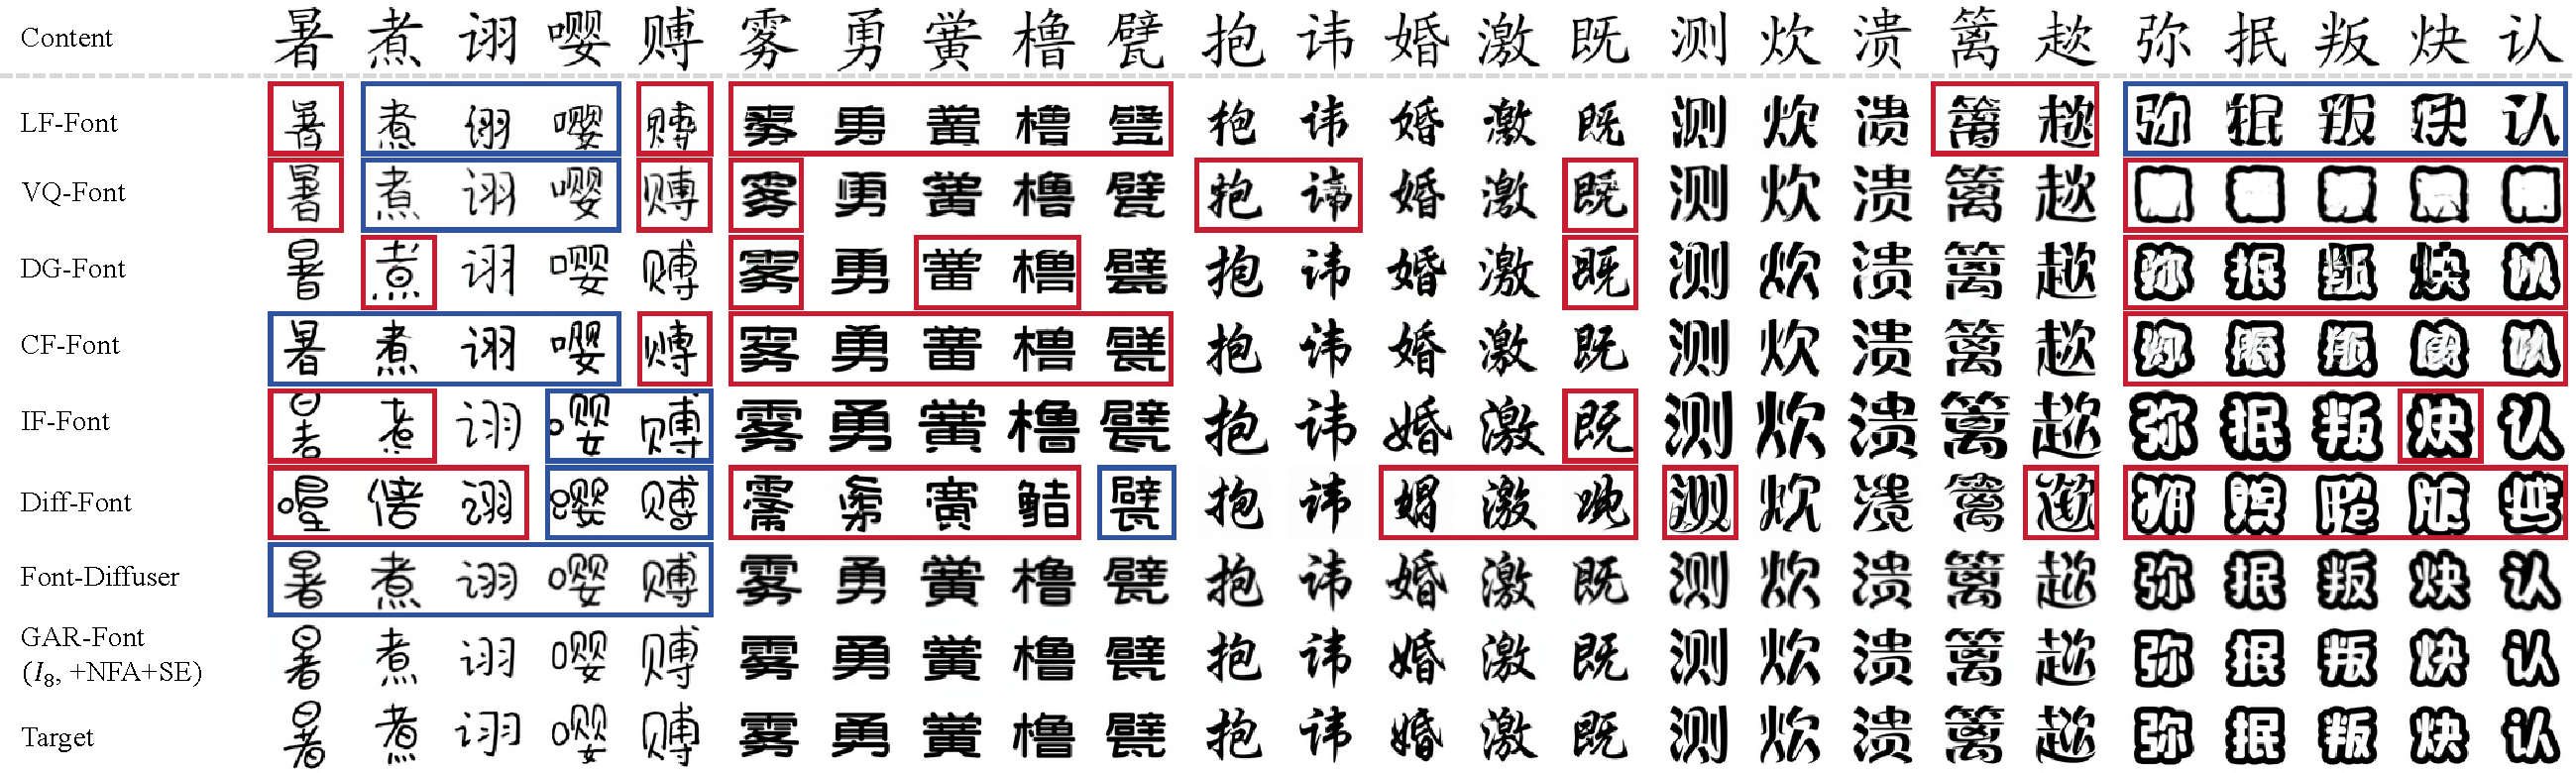
\includegraphics[width=0.95\linewidth]{IMGS/Exp1.pdf}
    \vspace{-3mm}
    \caption{Qualitative results on vision-only FFG (UFSC, \textit{Large} dataset). \textcolor{ex1figure_red}{\fbox{\rule{0pt}{4pt}\rule{4pt}{0pt}}} / \textcolor{ex1figure_blue}{\fbox{\rule{0pt}{4pt}\rule{4pt}{0pt}}} indicate structural errors and style mismatches. GAR-Font($I_8$, +NFA+SE) produces the most faithful glyphs with superior structure and style alignment.}
    \label{fig: Experiment1}
    \vspace{-3mm}
\end{figure*}

\section{Experiments}
\subsection{Datasets and Evaluation Metrics}
We evaluate GAR-Font and prior FFG methods on two datasets: a small-scale set containing 440 font styles (\textit{S}) and a large-scale set with 3,040 styles (\textit{L}). The small-scale dataset is a strict subset of the large-scale one, allowing fair cross-scale comparison. In each dataset, we randomly select 40 as unseen test fonts, while the remaining 400 (for \textit{S}) or 3,000 (for \textit{L}) are used for training.

Both datasets are constructed based on the official GB2312 character set, including 6,763 Chinese characters. Among them, 6,251 characters are randomly chosen for training, and the remaining 512 are held out as unseen characters. During evaluation, we consider two settings:

\noindent(1) \textit{Unseen Fonts Seen Characters (UFSC)}, where 512 seen characters are rendered with the 40 unseen fonts; and

\noindent(2) \textit{Unseen Fonts Unseen Characters (UFUC)}, where 512 unseen characters are rendered with the same unseen fonts.

We use RMSE$\downarrow$, SSIM$\uparrow$, LPIPS$\downarrow$, and FID$\downarrow$ to measure pixel- and perception-level similarity between generated and ground-truth glyphs. Following~\cite{LF_Font, HFH_Font}, we train a content classifier over 6,763 characters (99.71\% accuracy) and a font classifier over 3,040 fonts (92.72\% accuracy) to compute content accuracy (Acc(C)$\uparrow$) and style accuracy (Acc(S)$\uparrow$). All glyphs are resized to $64 \times 64$ for evaluation.

\subsection{Implementation Details}
The G-Tok tokenizer discretizes each glyph into 64 tokens using a 2,048-entry, dimension-8 codebook, trained for 200k iterations (batch = 16, lr = $1{\times}10^{-4}$). The vision-only AR generator uses the AdamW optimizer ($\beta_1 = 0.9$, $\beta_2 = 0.95$), conditioned on one Kaiti content. GAR-Font($I_8$) is trained with $N_s=8$ style glyphs for 600k/1M iterations on the small/large sets (batch = 32, lr = $1{\times}10^{-4}$).

For multimodal style encoder adaptation, the Language–style Adapter is trained for 40k iterations (batch size = 128, lr = $1{\times}10^{-4}$) with the visual-only features ($N_s=8$) as ground truth. By adjusting multimodal encoder's visual style reference numbers $k=2/4$, we build multimodal variants: GAR-Font($M_2$) and GAR-Font($M_4$).

In post-refinement, NFA is conducted on $128$ target font glyphs for $10$ epochs (lr = $2{\times}10^{-5}$). The SE phase is built upon GRPO, where each group generates $4$ samples and each character is trained with $8$ glyphs from different fonts (epochs = $10$, batch size = $32$, learning rate = $5\mathrm {e}{-6}$). 

%Our G-Tok tokenizer discretizes each glyph image into $64$ tokens with a codebook size of $2{,}048$, dimension of $8$ and is trained for $200$k iterations (batch size $16$, learning rate $1\mathrm{e}{-4}$). The vision-only AR generator is optimized using AdamW ($\beta_1{=}0.9$, $\beta_2{=}0.95$), conditioned on a Kaiti glyph as content reference and $n_{\text{ref}}{=}8$ style glyphs, . It is trained for $600$k iterations on the small-scale dataset and $1{,}000$k on the large-scale dataset (batch size $32$, learning rate $1\mathrm{e}{-4}$). The resulting model is denoted as GAR-Font($I_{8}$), indicating it takes $n_{\text{ref}}{=}8$ visual style glyphs as training inputs.

%After pretraining, we perform the post-refining stage on our vision-only AR generator. The NFA phase augments the model on $128$ glyphs of the target font for $10$ epochs (batch size $32$, learning rate $2\mathrm{e}{-5}$). The SE phase is built upon GRPO, where each group generates $4$ samples and each character is trained with $8$ glyphs from different fonts, for $10$ epochs (batch size $32$, learning rate $5\mathrm{e}{-6}$). 

%For our language-vision adapter, it is trained for $40$k iterations (batch size $128$, learning rate $1\mathrm{e}{-4}$) on the frozen GAR-Font($I_{8}$) pretrained on the large-scale dataset. The adapter is trained and evaluated under two configurations, GAR-Font($M_2$) ($\text{K}=2$) and GAR-Font($M_4$) $\text{K}=4$, where $\text{K}$ denotes the number of available style reference glyphs.

\subsection{Comparison on Few-shot Font Generation}
We conduct a comprehensive experiment in the \textbf{vision-only FFG} setting, where all models generate target glyphs using only reference images. GAR-Font($I_{8}$) is compared with seven open-source methods: GAN/VAE-based LF-Font~\cite{LF_Font}, VQ-Font~\cite{VQ_Font}, DG-Font~\cite{DG_Font}, CF-Font~\cite{CF_Font}; diffusion-based Diff-Font~\cite{Diff_Font} and Font-Diffuser~\cite{Font_Diffuser}; and the AR-based IF-Font~\cite{IF_Font}. All methods are trained and evaluated on the \textit{S} and \textit{L} datasets using their official resolutions and hyperparameters. GAR-Font($I_8$) is evaluated both before and after refinement (NFA and NFA+SE).

Table~\ref{tab:table1} shows that GAR-Font($I_{8}$) consistently outperforms existing vision-only FFG approaches. Even at the pretrained stage, it achieves competitive RMSE$\downarrow$ and SSIM$\uparrow$ on both \textit{UFSC}/\textit{UFUC}, and obtains the best FID$\downarrow$ scores on the large (\textit{L}) and small (\textit{S}) datasets. With NFA and SE, GAR-Font further improves in both style fidelity and structural accuracy, achieving RMSE$\downarrow$ ($0.2398/0.2508$) and SSIM$\uparrow$ ($0.6627/0.6377$) on \textit{UFSC}/\textit{UFUC}, surpassing existing methods by a large margin.

Figure~\ref{fig: Experiment1} presents comparisons under the \textit{UFSC} setting. GAR-Font($I_8$, +NFA+SE) generates the most precise and coherent glyphs. By contrast, LF-Font, VQ-Font, DG-Font, CF-Font, and Diff-Font often exhibit stroke distortion or structural collapse on complex styles. IF-Font frequently produces incomplete glyphs with overly thick strokes. Font-Diffuser maintains reasonable structure and style but tends to generate visibly blurred results.

%\chn{Figure~\ref{fig: Experiment1} displays the qualitative comparison on \textit{UFSC} of vision-only FFG methods trained on the large (\textit{L}) dataset. GAR-Font($I_8$, +NFA+SE) achieves the best performance, generating visually structurally precise and stylistically coherent results. In contrast, LF-Font, VQ-Font, DG-Font, CF-Font, and Diff-Font frequently suffer from stroke distortions or collapsed structures, especially on fonts with highly decorative designs. IF-Font often generates incomplete glyphs and presents overly thick strokes and enlarged structural frames. Although Font-Diffuser exhibits high structural fidelity and stylistic coherence, it tends to generate visibly blurred glyphs. More visualized results are provided in the supplementary material.} 

\begin{table*}[ht!]
\centering
\caption{
Quantitative results on multimodal FFG. GAR-Font($M_2$) and GAR-Font($M_4$) integrate textual style guidance with 2 or 4 visual references, outperforming vision-only baselines across all major metrics. Results demonstrate that language complements visual references, enhancing fine-grained style representation while reducing reliance on handcrafted visuals.}
\vspace{-2mm}
\setlength{\tabcolsep}{3pt}
\renewcommand{\arraystretch}{1.05}
\resizebox{0.9\textwidth}{!}{
\begin{tabular}{l | c c c c c c | c c c c c c }
\toprule
Method & \multicolumn{6}{c|}{Unseen Fonts Seen Characters (UFSC)} & \multicolumn{6}{c}{Unseen Fonts Unseen Characters (UFUC)} \\
\cmidrule(lr){2-7} \cmidrule(lr){8-13}
 & RMSE$\downarrow$ & SSIM$\uparrow$ & LPIPS$\downarrow$ & FID$\downarrow$ & Acc(C)$\uparrow$ & Acc(S)$\uparrow$
 & RMSE$\downarrow$ & SSIM$\uparrow$ & LPIPS$\downarrow$ & FID$\downarrow$ & Acc(C)$\uparrow$ & Acc(S)$\uparrow$ \\
\hline
$n_\text{ref} = 2$& 0.2816 & 0.5695 & 0.1158 & 7.3553 & 0.9184 & 0.1535 & 0.2825 & 0.5694 & 0.1162 & 7.5500 & 0.8930 & 0.1619 \\

$n_\text{ref} = 4$& 0.2807 & 0.5735 & 0.1138 & 7.3781 & 0.9206 & 0.1741 & 0.2813 & 0.5735 & 0.1146 & \textbf{7.4880} & 0.8958 & 0.1818 \\
$n_\text{ref} = 8$& 0.2772 & 0.5799 & 0.1112 & 7.7155 & 0.9146 & \textbf{0.1928} & 0.2784 & 0.5787 & 0.1121 & 8.0349 & 0.8912 & \textbf{0.1892} \\
\Xhline{1.2pt}
GAR-Font($M_2$)  & 0.2811 & 0.5724 & 0.1136 & \textbf{7.3145} & \textbf{0.9296} & 0.1203
                 & 0.2817 & 0.5731 & 0.1143 & 7.5306 & \textbf{0.9068} & 0.1289 \\

GAR-Font($M_4$)   & \textbf{0.2764} & \textbf{0.5825} & \textbf{0.1098} & 7.4915 & 0.9260 & 0.1688 
                 & \textbf{0.2776} & \textbf{0.5816} & \textbf{0.1107} & 7.6607 & 0.9039 & 0.1744 \\
\bottomrule
\end{tabular}
}
\label{tab:adapter_experiment}
\vspace{-3mm}
\end{table*}
\subsection{Efficient Vision-Language Adaptation}
We further evaluate \textbf{multimodal FFG} to assess whether textual style descriptions can improve over vision-only references. Using GAR-Font($I_8$) on the large (\textit{L}) dataset, we vary the number of visual references $n_\text{ref}\in{2,4,8}$ as baselines. We then introduce multimodal variants GAR-Font($M_2$) and GAR-Font($M_4$), which pair 2 or 4 visual references with one textual style description obtained via Qwen2.5-VL~\cite{Qwen25VL} captioning; further details are provided in the supplementary material.

As shown in Table~\ref{tab:adapter_experiment}, both multimodal models outperform their vision-only counterparts with the same number of visual references across all major metrics. GAR-Font($M_4$) even surpasses the 8-reference visual model, achieving lower RMSE$\downarrow$/LPIPS$\downarrow$ and higher SSIM$\uparrow$ on the \textit{UFSC}, along with a better FID$\downarrow$ ($7.4915$ vs. $7.7155$). Similar gains appear on \textit{UFUC}, confirming that language provides complementary style cues and reduces reliance on numerous visual references. A mild decrease in ACC(S) is observed, likely because textual guidance yields smoother and more diverse styles beyond the classifier’s limit.

Qualitative examples in Figure~\ref{fig: Experiment2} show that GAR-Font($M_2$) and GAR-Font($M_4$) preserve styles more reliably than vision-only models, particularly when $n_\text{ref}=2$, where the visual baseline noticeably drifts toward generic shapes. This highlights the effectiveness of language in reinforcing style fidelity under low-reference conditions.


%both multimodal variants outperform their vision-only counterparts with the same visual reference numbers across all major metrics. GAR-Font($M_4$) achieves superior RMSE$\downarrow$/SSIM$\uparrow$/LPIPS$\downarrow$ results of $0.2764/0.5825/0.1098$ on the \textit{UFSC} split, surpassing the 8-reference visual model GAR-Font($I_8$) ($0.2772/0.5799/0.1112$) while maintaining superior FID$\downarrow$ ($7.4915$ vs. $7.7155$). Similar gains appear on \textit{UFUC}, indicating that textual style descriptions complement visual references to enhance fine-grained style representation. This also validates the lightweight multimodal style guidance, enabling flexible language-driven control and reducing reliance on more handcrafted visuals. Meanwhile, we note a slight drop in ACC(S), likely due to textual guidance producing smoother, more diverse styles that deviate from the limited categories learned by the style classifier. \chn{Qualitative comparisons can be viewed in Figure ~\ref{fig: Experiment2}. Under textual style guidance, GAR-Font($M_2$) and GAR-Font($M_4$) generate glyphs with more coherent style and finer structural integrity. Notably, when $n_\text{ref}=2$, the vision-only model exhibits visible style degradation, with some generated glyphs partially regressing toward a generic Song-like appearance and losing distinctive stylistic features. In contrast, the multimodal GAR-Font($M_2$), guided by textual descriptions, preserves the target style more effectively, highlighting the complementary role of language in refining style fidelity.}

\subsection{Ablation Studies}
\subsubsection{On G-Tok's Hybrid Architecture}
To validate G-Tok's hybrid CNN-ViT design, we start from a CNN-based tokenizer~\cite{llamagen} and progressively insert ViT blocks at different depths to introduce global awareness.

We conduct two complementary analyses on \textit{UFUC} test:
\begin{enumerate}
\item \textbf{Linear Probing} evaluates the discriminative quality of frozen G-Tok representations for style and content prediction using a single-layer linear classifier. Features are extracted and flattened from the frozen tokenizer encoder, and high classification accuracy indicates that the encoder effectively captures and discriminates structural and stylistic information.
\item \textbf{Reconstruction Robustness} recovers glyphs corrupted by localized Gaussian noise ($\sigma = 0.2$, affecting 20\% of the glyph area). High performance indicates that the tokenizer effectively preserves global structure and stylistic cues despite local perturbations.
\end{enumerate}
Table~\ref{tab:ablation_linear_robust_combined} shows that the pure ViT excels in linear probing but suffers in reconstruction, while the CNN baseline ensures stable recreation with weaker probing results. The hybrid G-Tok progressively integrates global attention, with the CNN-ViT-6 variant achieving the best, improving both classification accuracy and reconstruction fidelity across all metrics. Visualizations are in the supplementary material.

%\begin{enumerate}
%\item \textbf{Linear Probing} evaluates the discriminative quality of frozen G-Tok representations for style and content prediction using a simple linear classifier.
%\item \textbf{Robust Reconstruction} assesses reconstruction robustness on noised glyphs with localized Gaussians ($\sigma = 0.2$, covering 20\% of the area).
%\end{enumerate}
%To validate the G-Tok's of our hybrid CNN-ViT architecture within G-Tok, we start from the CNN-based tokenizer modified from the tokenizer in~\cite{llamagen}, and progressively insert Transformer blocks at different depths to introduce global-awareness.

%We perform two complementary analyses on the UFUC test set to evaluate G-Tok:
%\begin{enumerate}
%    \item \textbf{Linear Probing:} We evaluate the discriminative quality of G-Tok's learned global structural and stylistic representations by training a simple linear classifier for style and content prediction using the frozen encoder weights.
%    \item \textbf{Robust Global Reconstruction:} We further evaluate the model’s robustness by reconstructing glyphs from inputs corrupted with localized Gaussian noise (standard deviation 0.2) covering 20\% of the glyph area.
%\end{enumerate}

%As shown in Table~\ref{tab:ablation_linear_robust_combined}, the pure ViT model exhibits strong discriminative capability in linear probing but suffers from degraded reconstruction quality due to the lack of fine-grained spatial representations. In contrast, the CNN baseline achieves stable reconstruction yet limited global representation ability. Our hybrid G-Tok progressively integrates global attention, and the CNN-ViT-6 variant achieves the best balance, improving both classification accuracy and reconstruction fidelity across all metrics.


\begin{table}[t]
\centering
\caption{
Ablation of G-Tok's hybrid CNN-ViT architecture on \textit{UFUC}. \textbf{Bold} and \underline{underline} indicate the best and second-best results. Progressive integration of global attention improves both discriminative representation and reconstruction fidelity.
}
\vspace{-2mm}
\renewcommand{\arraystretch}{1.1}
\resizebox{0.47\textwidth}{!}{
\begin{tabular}{l | c c | c c c c }
\toprule
Method & \multicolumn{2}{c|}{Linear Probing} & \multicolumn{4}{c}{Reconstruction Robustness} \\
\cmidrule(lr){2-3} \cmidrule(lr){4-7}
 & Acc(S)$\uparrow$ & Acc(C)$\uparrow$ & RMSE$\downarrow$ & SSIM$\uparrow$ & LPIPS$\downarrow$ & FID$\downarrow$ \\
\hline
CNN       & 0.5515 & 0.3879 & 0.1167 & 0.8535 & 0.0423 & 28.4279 \\
ViT-6       & \textbf{0.6907} & \textbf{0.5334} & 0.1636 & 0.7333 & 0.0933 & 98.4270 \\
CNN-ViT-2 & 0.5229 & 0.3772 & 0.1114 & 0.8552 & \underline{0.0420} & 30.0034 \\
CNN-ViT-4 & 0.5585 & 0.3667 & \underline{0.1114} & \underline{0.8563} & 0.0430 & \underline{24.7323} \\
CNN-ViT-6 & \underline{0.6277} &\underline{0.4897} & \textbf{0.1088} & \textbf{0.8594} & \textbf{0.0412} & \textbf{22.1577}\\
\bottomrule
\end{tabular}
}
\label{tab:ablation_linear_robust_combined}
\vspace{-3mm}
\end{table}

%\chn{Visual comparisons of robust reconstruction can be viewd at Figure..., which demonstrate G-Tok's global modeling capability with resilience to local perturbations.}

\subsubsection{On G-Tok's Global and Causal Modeling}
% CNN, CNN+Non-Causal ViT, CNN + Causal ViT 
% To evaluate the impact of global-aware and causal modeling within our G-Tok, we pretrained three visual AR generator variants: (1) CNN, (2) CNN+Non-causal ViT, and (3) CNN+Causal ViT, where the causal ViT is applied only in the decoder to model sequential dependencies among quantized tokens. 
We further ablate G-Tok's ViT architecture to assess its global and causal modeling. We pretrain three visual AR variants that differ in G-Tok and examine them on \textit{UFUC}: % \chn{on the small (\textit{S}) dataset} ?
\begin{enumerate}
\item \textbf{CNN:} a baseline CNN tokenizer without global context;
\item \textbf{CNN + Non-causal ViT:} a hybrid CNN-ViT tokenizer with self-attention that only supports global interaction;
\item \textbf{CNN + Causal ViT:} full G-Tok, hybrid CNN-ViT tokenizer with causal self-attention for sequential modeling.
\end{enumerate}
Table~\ref{tab:ablation_gtok_generator} shows that incorporating self-attention ViT improves performance over the CNN baseline, while the causal ViT further enhances sequential modeling, achieving the best results across all metrics. Detailed \textit{UFSC} results are provided in the supplementary material.

%As shown in Table~\ref{tab:ablation_gtok_generator}, introducing ViT modules into the tokenizer improves the generation quality. Compared with the CNN baseline, the hybrid CNN-ViT variants achieve better metrics, demonstrating this kind of hybrid global-aware tokenizer effectively captures structural and stylistic patterns, which are essential in font synthesis. Furthermore, adopting causal self-attention within the tokenizer's ViT decoder enhances sequential token modeling during reconstruction, leading to additional improvements in glyph fidelity.

\begin{table}[t]
\centering
\caption{Ablation of G-Tok’s architecture on \textit{UFUC}. Incorporating self-attention (CNN+Non-Causal ViT) improves global context modeling while causal attention further strengthens sequential modeling, yielding the best performance across all metrics.}
\vspace{-3mm}
\setlength{\tabcolsep}{3pt}
\renewcommand{\arraystretch}{1.05}
\resizebox{0.475\textwidth}{!}{
\begin{tabular}{l | c c c c c c }
\toprule
Method & RMSE$\downarrow$ & SSIM$\uparrow$ & LPIPS$\downarrow$ & FID$\downarrow$ & Acc(C)$\uparrow$ & Acc(S)$\uparrow$ \\
\hline
CNN & 0.3447 & 0.4350 & 0.1728 & 10.5239 & 0.6722 & 0.0221 \\
CNN+Non-Causal ViT & 0.3271 & 0.4745 & 0.1562 & 8.7504 & 0.8019 & 0.0436 \\
CNN+Causal ViT & \textbf{0.3142} & \textbf{0.4932} & \textbf{0.1421} & \textbf{8.4841} & \textbf{0.8993} & \textbf{0.0796} \\
\bottomrule
\end{tabular}
}
\label{tab:ablation_gtok_generator}
\vspace{-3mm}
\end{table}
\begin{table*}[t]
\centering
\caption{
Ablation of decoding strategy and pixel-level supervision on UFSC and UFUC.
Soft decoding outperforms hard decoding across all metrics, and pixel supervision further enhances reconstruction fidelity and recognition accuracy.
}
\vspace{-2mm}
\setlength{\tabcolsep}{3pt}
\renewcommand{\arraystretch}{1.05}
\resizebox{0.9\textwidth}{!}{
\begin{tabular}{l |c| c c c c c c | c c c c c c }
\toprule
Training Loss & Decoding &\multicolumn{6}{c|}{Unseen Fonts Seen Characters (UFSC)} & \multicolumn{6}{c}{Unseen Fonts Unseen Characters (UFUC)} \\
\cmidrule(lr){3-8} \cmidrule(lr){9-14}
& Strategy & RMSE$\downarrow$ & SSIM$\uparrow$ & LPIPS$\downarrow$ & FID$\downarrow$ & Acc(C)$\uparrow$ & Acc(S)$\uparrow$ & 
RMSE$\downarrow$ & SSIM$\uparrow$ & LPIPS$\downarrow$ & FID$\downarrow$ & Acc(C)$\uparrow$ & Acc(S)$\uparrow$ \\
\hline
w/o pixel loss & hard & 0.3235 & 0.4679 & 0.1517 & 10.3181 & 0.8647 & 0.0377 & 0.3322 & 0.4510 & 0.1602 & 11.2142 & 0.7465 & 0.0396 \\

         & soft & 0.3231 & 0.4745 & 0.1502 & 9.6696 & 0.9171 & 0.0426 & 0.3313 & 0.4583 & 0.1589 & 10.3813 & 0.8104 & 0.0430 \\
\hline
w/ pixel loss & hard & 0.3083 & 0.4991 & 0.1329 & 8.3024 & 0.9032 & 0.0771 & 0.3157 & 0.4862 & 0.1448 & 8.9043 & 0.8404 & 0.0680 \\

 & soft & \textbf{0.3080} & \textbf{0.5052} & \textbf{0.1313} & \textbf{7.9484} & \textbf{0.9408} & \textbf{0.0802} & \textbf{0.3142} & \textbf{0.4932} & \textbf{0.1421} & \textbf{8.4841} & \textbf{0.8993} & \textbf{0.0796} \\

\bottomrule
\end{tabular}
}
\label{tab:ablation_decode_strategy}
\vspace{-2mm}
\end{table*}
\begin{table*}[ht!]
\centering
\caption{
Quantitative comparison of joint training (GAR-Font($VL_k$)) versus the decoupled adapter scheme (GAR-Font($M_k$)) on unseen fonts. The decoupled Language-style Adapter surpasses joint-trained multimodal encoders, validating more effective vision–language alignment and improved reconstruction and perceptual metrics.
}
\vspace{-3mm}
\setlength{\tabcolsep}{3pt}
\renewcommand{\arraystretch}{1.05}
\resizebox{0.9\textwidth}{!}{
\begin{tabular}{l | c c c c c c | c c c c c c }
\toprule
Method & \multicolumn{6}{c|}{Unseen Fonts Seen Characters (UFSC)} & \multicolumn{6}{c}{Unseen Fonts Unseen Characters (UFUC)} \\
\cmidrule(lr){2-7} \cmidrule(lr){8-13}
 & RMSE$\downarrow$ & SSIM$\uparrow$ & LPIPS$\downarrow$ & FID$\downarrow$ & Acc(C)$\uparrow$ & Acc(S)$\uparrow$
 & RMSE$\downarrow$ & SSIM$\uparrow$ & LPIPS$\downarrow$ & FID$\downarrow$ & Acc(C)$\uparrow$ & Acc(S)$\uparrow$ \\
\hline
GAR-Font($VL_2$)  & 0.3070 & 0.5124 & 0.1458 & 10.7566 & 0.8552 & 0.1104
                 & 0.3100 & 0.5087 & 0.1473 & 11.0381 & 0.7979 & 0.1209 \\

GAR-Font($VL_4$)  & 0.2983 & 0.5378 & 0.1279 & 7.9272 & 0.8970 & 0.1165
                 & 0.3006 & 0.5351 & 0.1290 & 8.1126 & 0.8665 & 0.1216 \\

GAR-Font($M_2$)  & 0.2811 & 0.5724 & 0.1136 & \textbf{7.3145} & \textbf{0.9296} & 0.1203
                 & 0.2817 & 0.5731 & 0.1143 & 7.5306 & \textbf{0.9068} & 0.1289 \\

GAR-Font($M_4$)  & \textbf{0.2764} & \textbf{0.5825} & \textbf{0.1098} & 7.4915 & 0.9260 & 0.1688 
                 & \textbf{0.2776} & \textbf{0.5816} & \textbf{0.1107} & 7.6607 & 0.9039 & 0.1744 \\
\bottomrule
\end{tabular}
}
\label{tab:generator_with_adapter_experiment}
\end{table*}
\begin{figure*}[!t]
    \centering
    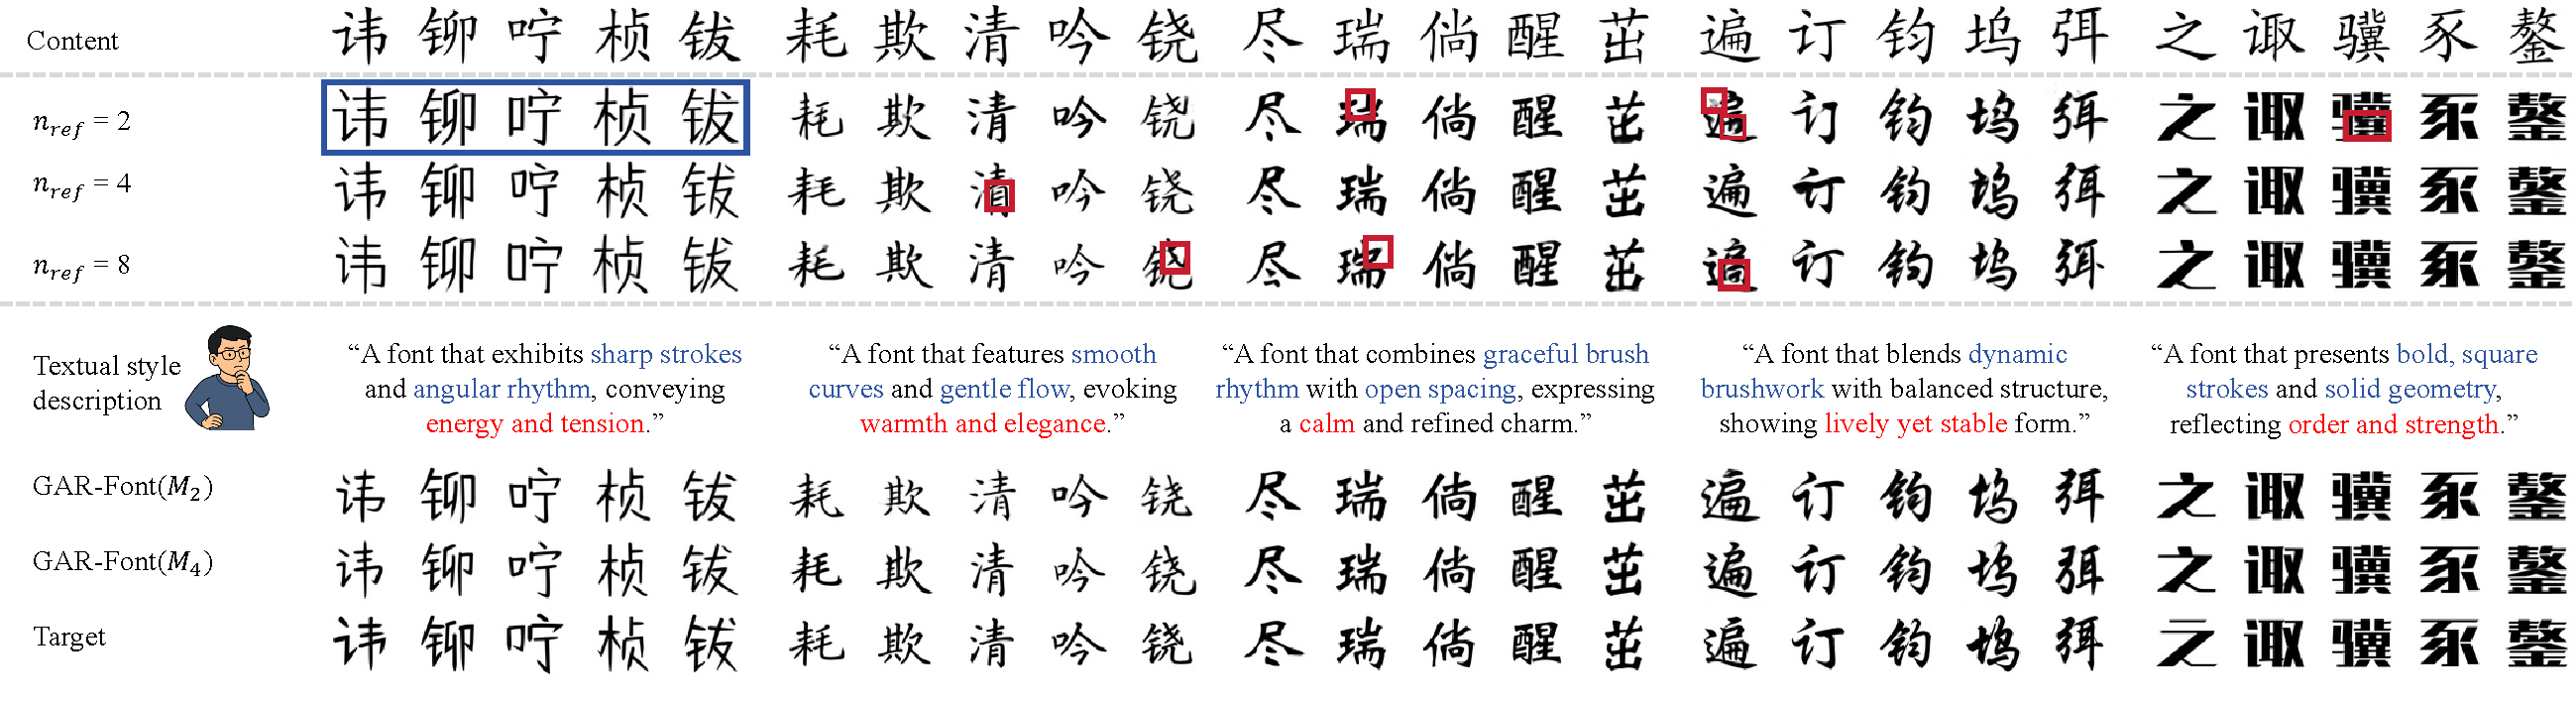
\includegraphics[width=0.95\linewidth]{IMGS/Exp2.pdf}
    \vspace{-5mm}
    \caption{Qualitative results on multimodal FFG(UFSC, \textit{Large} dataset). \textcolor{ex2figure_red}{\fbox{\rule{0pt}{4pt}\rule{4pt}{0pt}}} denotes local slight structural mistakes and \textcolor{ex2figure_blue}{\fbox{\rule{0pt}{4pt}\rule{4pt}{0pt}}} marks samples with stylistic regression. With textual style guidance, GAR-Font($M_2$) and GAR-Font($M_4$) yield more structurally accurate and stylistically coherent generations, demonstrating enhanced stable fine-grained style control over vision-only baselines.} 
    \label{fig: Experiment2}
    \vspace{-3mm}
\end{figure*}

\subsubsection{On AR Generator's Soft-decoding}
To validate the effectiveness of pixel-level supervision and the soft decoding strategy, we conduct ablation experiments on our vision-only AR generator.
The results in Table~\ref{tab:ablation_decode_strategy} demonstrate that soft decoding achieves superior performance over all metrics, particularly when combined with pixel-level supervision. 
This combination yields the lowest RMSE$\downarrow$, LPIPS$\downarrow$, and FID$\downarrow$ while achieving the highest SSIM$\uparrow$ and recognition accuracies on both \textit{UFSC} and \textit{UFUC}, indicating improved pixel-level fidelity and design fidelity. %\lyx{Visual comparisons in Figure~\ref{fig:soft_decode_vis}, which further illustrate the perceptual advantages of soft decoding.}


\subsubsection{On Multimodal Style Encoder's Adaptation}
%GAR-Font adopts a decoupled training paradigm: we first pretrain a visual encoder and then extend it to multimodal control via a lightweight Language-style Adapter. To validate this design, we compare this decoupled scheme with joint training of a multimodal style encoder using the same configuration as GAR-Font($I_8$) on the large (\textit{L}) dataset.
GAR-Font adopts a decoupled training paradigm: we first pretrain a visual encoder and then introduce multimodal control via a lightweight Language-style Adapter. To validate this design, we compare it with jointly training a multimodal style encoder under the same GAR-Font($I_8$) configuration on the large (\textit{L}) dataset.

Concretely, we evaluate two joint training variants, \textbf{GAR-Font($VL_2$)} and \textbf{GAR-Font($VL_4$)}, against the decoupled multimodal variants \textbf{GAR-Font($M_2$)} and \textbf{GAR-Font($M_4$)}. As displayed in Table~\ref{tab:generator_with_adapter_experiment}, the decoupled variants consistently outperform their joint-trained counterparts under the same number of visual references. For example, GAR-Font($M_4$) attains the best RMSE$\downarrow$, LPIPS$\downarrow$, and SSIM$\uparrow$ on \textit{UFSC} / \textit{UFUC}, while GAR-Font($VL_4$) yields notably worse RMSE$\downarrow$ and SSIM$\uparrow$. GAR-Font($M_2$) also achieves the best FID$\downarrow$ on \textit{UFSC} ($7.3145$). These results validate the decoupled vision–language training paradigm, where a pretrained visual encoder and a lightweight adapter achieve efficient and robust text–visual alignment, improving generalization in multimodal FFG.

%Concretely, we evaluate two joint training variants, \textbf{GAR-Font($VL_2$)} and \textbf{GAR-Font($VL_4$)}, against the decoupled multimodal variants \textbf{GAR-Font($M_2$)} and \textbf{GAR-Font($M_4$)}. As displayed in Table~\ref{tab:generator_with_adapter_experiment}, the decoupled variants consistently outperform their joint-trained counterparts under the same number of visual references. For example, GAR-Font($M_4$) attains the lowest RMSE ($0.2764 / 0.2776$), the lowest LPIPS ($0.1098 / 0.1107$), and the highest SSIM ($0.5825 / 0.5816$) on \textit{UFSC} / \textit{UFUC}, while GAR-Font($VL_4$) yields notably worse RMSE and SSIM ($0.2983 / 0.3006$ and $0.5378 / 0.5351$, respectively). GAR-Font($M_2$) also achieves the best FID on \textit{UFSC} ($7.3145$).

%These results validate the decoupled vision–language training paradigm, where a pretrained visual encoder and a lightweight adapter achieve efficient and robust text–visual alignment, improving generalization in multimodal FFG.

%\subsubsection{On Multimodal Style Encoder's Adaptation}
%GAR-Font follows a decoupled training paradigm that first learns visual encoder and extend it to multimodal control through a Language-style Adapter. 为了验证这个设计的合理性，们对比了相同configuration下直接训练multimodal style encoder from scratch的实验。 

%To evaluate the effectiveness the vision-language decoupled training paradigm of GAR-Font, we further conduct an ablation study using the same training configuration as GAR-Font($I_8$) trained on the large (\textit{L}) dataset. We introduce two joint-training variants, \textbf{GAR-Font($VL_2$)} and \textbf{GAR-Font($VL_4$)}, which are trained with both textual style descriptions and $N_s=2,4$ visual style references.

%As shown in Table~\ref{tab:generator_with_adapter_experiment}, both jointly trained variants GAR-Font($VL_2$) and GAR-Font($VL_4$) perform worse than their decoupled multimodal counterparts GAR-Font($M_2$) and GAR-Font($M_4$) under the same number of visual references. Specifically, our GAR-Font($M_4$) achieves the lowest RMSE ($0.2764/0.2776$), LPIPS ($0.1098/0.5816$) and the highest SSIM ($0.5825/0.5816$) under UFSC/UFUC settings. These results validate the effectiveness of the decoupled vision-language training method, which not only enables efficient alignment between textual and visual representations but also enhances the robustness and generalization of multimodal font generation.


\subsection{Limitations and Future Work.}
Although GAR-Font surpasses existing FFG methods in visual fidelity and structural preservation, several limitations remain. First, the Multimodal Style Encoder currently relies on late adaptation via a language-style adapter; exploring earlier text-image fusion could enable finer stylistic control and reduce reliance on visual references. Scaling the model to larger sizes is also left for future work. Second, GAR-Font is limited to $64 \times 64$ outputs, restricting high-DPI applications; higher-resolution generation will require redesigning G-Tok to handle longer token sequences efficiently. Finally, we aim to expand controllability beyond style and content, adding attributes like stroke thickness, character width, and slant for more flexible font generation.


%\subsection{Limitations and Future Work.}
%Although our vision-only model outperforms existing FFG methods in preserving visual fidelity and structural details, GAR-Font is still faced with limitations handling structures of some complex glyphs, where the generated results may exhibit slight stroke distortions. This degradation is likely attributed to error accumulation during the AR modeling. Future work may address this by incorporating structure-aware priors to enhance robustness on complex glyphs. 



%\subsection{Datasets and Evaluation Metrics}
%To comprehensively evaluate the effectiveness and scalability of GAR-Font and existing FFG methods, we construct two \lyx{training?} datasets derived from the GB2312 standard character set (6,763 Chinese characters): a small-scale dataset with 440 fonts and a large-scale dataset with 3,040 fonts. The small dataset is a strict subset of the large one to ensure fair cross-scale comparison. We randomly select 40 fonts as testing unseen fonts, and the remaining fonts (400/3,000) are used for training. A unified character split of the GB2312 set is applied across all fonts, with 6,251 characters for training and 512 unseen characters for testing. During evaluation, we further sample 512 characters from the training set and combine them with the 512 unseen characters to form two test settings: SeenCharacters and UnseenCharacters. All evaluations are conducted on the 40 unseen fonts to assess the generalization across both style and content domains.

%To evaluate performance quantitatively, we employ RMSE, SSIM, LPIPS, and FID to assess the pixel-level and perception-level similarity between the generated and ground-truth glyphs. Following prior works ~\cite{LF_Font, HFH_Font}, we further train a content classifier over 6,763 classes of characters with 99.71\% accuracy and a font classifier over 3,040 classes of fonts with 92.72\% accuracy to compute content accuracy $(ACC(C))$ and style accuracy $(ACC(S))$ as important metrics. All generated glyph images are resized to $64 \times 64$ for fair evaluation.
 

%\subsection{Implemention Details}
%Our G-Tok discretizes the glyph images into $64$ tokens with the size of codebook setting to $2,048$ and is trained for $200$k iterations (batch size $16$, learning rate 1e-4). The autoregressive generator is optimized by Adam~\cite{Adam} ($\beta_1{=}0.9$, $\beta_2{=}0.95$) for $800$k, conditioned on a Kaiti glyph as the content reference and $n_{\text{ref}}{=}8$ style glyphs, and trained for $600$k iterations on the small-scale dataset and $1{,}000$k iterations on the large-scale dataset. (batch size $32$, learning rate 1e-4). After pretraining, we conduct post-training process. The SFT phase fine-tunes model on  $128$ glyph images of the target font with $10$ epochs(batch size $32$, learning rate $2e-5$). The RL phase employs GRPO, with each group generating $4$ samples, and is trained for $10$ epochs (batch size $32$, learning rate 5e-6), where each character is trained with $8$ glyphs of different training fonts. For the style-language adapter, it is trained for $40$k iterations (batch size $128$, learning rate 1e-4) on a frozen generator pretrained on the large-scale dataset to align textual and visual fine-grained style features.

%\subsection{Comparison with State-of-the-Art Methods}
%We compare our GAR-Font with 8 state-of-the-art font generation methods, including four GAN/VAE-based models: LF-Font ~\cite{LF_Font}, VQ-Font ~\cite{VQ_Font}, DG-Font ~\cite{DG_Font}, CF-Font ~\cite{CF_Font}, three diffusion-based models: Diff-Font ~\cite{Diff_Font}, Font-Diffuser ~\cite{Font_Diffuser}, HFH-Font ~\cite{HFH_Font}, and one autoregressive model: IF-Font ~\cite{IF_Font}. To be fair, We retain the default settings in their papers and source codes on our dataset, including resolution and optimization hyperparameters. Since most existing methods do not support few-shot fine-tuning in their provided codes, we additionally fine-tune the current best-performing baseline, HFH-Font with our protocal for a fair comparison. Our GAR-Font models are evaluated under both pretraining and post-training(SFT and SFT+RL) settings.


%\paragraph{Quantitative Results.}  
%As shown in Table~\ref{tab:table1}, our GAR-Font demonstrates excellent performance compared with existing state-of-the-art FFG methods. In the pretrained stage, GAR-Font has already outperformed most methods. On the small dataset, with competitive RMSE ($0.2772/0.2784$) and SSIM ($0.5799/0.5787$), the pretrained model achieves FID of $7.9484/8.4841$ on UFSC/UFSC, while on the large dataset it achieves $7.7155/8.0349$ on UFSC/UFUC, ranking only behind HFH-Font.

%After post-training with SFT and RL, GAR-Font shows substantial improvements and surpasses HFH-Font on several key metrics. On the small dataset, GAR-Font outperforms HFH-Font on UFSC and achieves comparable metrics on UFUC. On the large dataset, GAR-Font achieves RMSE $0.2398/0.2503$ and SSIM $0.6627/0.6380$ on UFSC/UFUC (vs. $0.2645/0.2622$ and $0.6211/0.6259$ for HFH-Font(SFT)), outperforming by a considerable margin.
\vspace{-2mm}
\section{Conclusion}
\vspace{-2mm}
In this paper, we present GAR-Font, a global-aware autoregressive framework for few-shot font generation that combines a hybrid global tokenizer, an autoregressive generator with a multimodal style encoder, and a post-refinement pipeline. GAR-Font achieves superior structural and stylistic fidelity, outperforming prior vision-only baselines, while demonstrating that language-guided adaptation can rival or exceed heavy visual conditioning with improved flexibility.

%In this paper, we presented GAR-Font, a global-aware autoregressive framework that advances few-shot font generation through global modeling and lightweight multimodal alignment. By jointly leveraging a hybrid CNN–ViT tokenizer (G-Tok), an autoregressive generator with a multimodal style encoder, and a post-refinement pipeline (NFA+SE), GAR-Font achieves superior structural fidelity and stylistic fidelity. Extensive experiments show that GAR-Font outperforms prior vision-only and multimodal baselines and that language-guided adaptation can match or exceed heavy visual conditioning while enabling flexible control.
\clearpage
\setcounter{page}{1}
\setcounter{section}{0}
\setcounter{figure}{0}
\setcounter{table}{0}
\maketitlesupplementary
\renewcommand\thesection{\Alph{section}}
\renewcommand{\thetable}{S\arabic{table}}    % 修改表格标签
\renewcommand{\thefigure}{S\arabic{figure}}  % 修改图片标签

\section{Overview}
\vspace{-1mm}
This supplementary material provides additional details on dataset construction, implementation, and extended experiments supporting the main paper. The sections are organized as follows:
\begin{itemize}
    \item \textbf{\cref{sec:models}}: Model configurations of G-Tok, the autoregressive generator, and the multimodal style encoder.
    \item \textbf{\cref{sec:data_dist}}: Data curation and partitioning, covering both training and evaluation protocols.
    \item \textbf{\cref{sec:quant_ext}}: Extended quantitative results, including scaling analyses of our autoregressive generator.
    \item \textbf{\cref{sec:Ablate}}: Detailed and visualized ablations of key design choices in GAR-Font.
    \item \textbf{\cref{sec:vis_results}}: Extensive qualitative results for visual-only and multimodal FFG, along with error analyses.
    \item \textbf{\cref{sec:Failure_cases}}: Analysis of GAR-Font failure cases in dense-stroke and complex font styles.

    
\end{itemize}

%%%%%%%%%%%%%%%%%%%%%%%%%
\section{Model Configuration}
\label{sec:models}
Table~\ref{tab:model-structure} details the architectural specifications of GAR-Font. The framework relies on three core components: (1) The \textbf{Global-aware Tokenizer (G-Tok)} , which employs a hybrid CNN-ViT architecture to discretize glyphs into a compact codebook ($N=2048$); (2) The \textbf{Autoregressive Generator}, which serves as the synthesis backbone, using a deep Transformer decoder to predict tokens conditioned on aggregated content and style features; and (3) The \textbf{Multimodal Style Encoder}, which utilizes a lightweight adapter to align textual embeddings with visual style representations for text-driven control.
\begin{table}[h]
\centering
\small
\setlength{\tabcolsep}{3pt} % 调小列间距
\begin{tabular}{p{0.8\columnwidth} c}
\toprule
\textbf{Key Components} & \textbf{Params (M)} \\
\midrule
\textbf{G-Tok} & 79.59 \\
CNN Encoder & 28.56 \\
ViT Encoder (layers = 6) & 4.73 \\
Codebook (size = 2048, dim = 8) & 0.02 \\
ViT Decoder (layers = 6) & 4.73 \\
CNN Decoder & 41.42 \\
\midrule
\textbf{AR-Generator} &  346.23 \\
Content Encoder & 28.56 \\
Visual Style Encoder & 2.78 \\
Content-style Aggregator (layers = 3) & 0.79 \\
Transformer Decoder (layers = 24) & 314.10 \\
\midrule
\textbf{Multimodal Style Encoder} & 8.04 \\
Projection & 0.52 \\
Visual Style Encoder & 2.78 \\
Language-Style Adapter (layers = 6) & 4.74 \\
\bottomrule
\end{tabular}
\vspace{-3mm}
\caption{Key GAR-Font components and parameter counts.}
\vspace{-3mm}
\label{tab:model-structure}
\end{table}
\begin{figure}[t]
  \centering
  % You will insert the python-generated PDF here
  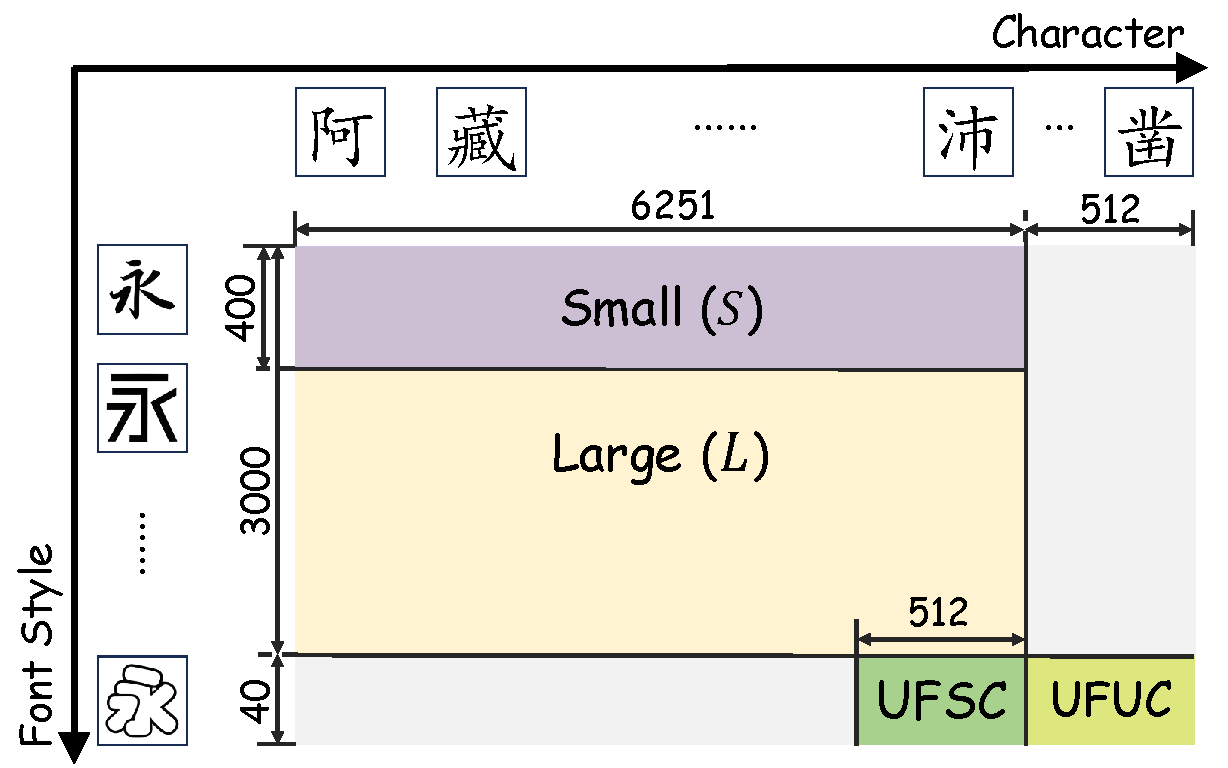
\includegraphics[width=0.95\linewidth]{SUPP_IMGS/data_visualization.pdf} 
  \vspace{-3mm}
  \caption{\textbf{Visual illustration of the dataset partition.} The data is organized along font and character axes. Pre-training utilizes the purple and yellow regions ($S$ and $L$). Evaluation is conducted on the bottom green regions (\textit{UFSC} and \textit{UFUC}), strictly isolating unseen styles and characters.}
  \vspace{-3mm}
  \label{fig:data_viz}
\end{figure}


\section{Data Curation}
\label{sec:data_dist}

\subsection{Data Collection and Statistics}
\label{ssec:data_stats}
We construct a comprehensive font dataset derived from the official GB2312 character set. As illustrated in \cref{fig:data_viz}, the whole training and test dataset is structured as a matrix spanned by two orthogonal axes: \textit{Font Style} (vertical axis) and \textit{Character Category} (horizontal axis). 
The collected data comprises 3,040 fonts and 6,763 characters. 

For training data, along the Character Axis, we split 6,251 training characters (left column) and left 512 characters unseen (right column). The unseen characters are reserved strictly for testing to evaluate the model's capability to generate novel glyph structures. Similarly, the font library is divided into 3,000 training fonts (top rows) and 40 unseen test fonts (bottom rows).


\subsection{Pretraining Data}
\label{ssec:data_pretrain}
The pretraining phase utilizes the data located in the upper-left quadrant of \cref{fig:data_viz}, defined by the intersection of training fonts and training characters. Within this quadrant, we define two configurations to investigate scaling behaviors:
\begin{itemize}[leftmargin=*]
    \item Large ($L$): The full training block consisting of all 3,000 training fonts paired with the 6,251 training characters (represented by the blue region).
    \item Small ($S$): A subset consisting of the first 400 training fonts paired with the same 6,251 characters (represented by the reddish overlay).
\end{itemize}
Training on $S$ versus $L$ allows us to assess the model's data efficiency and performance scaling with respect to the diversity of source styles.

\subsection{Textual Prompt Collection}
\label{ssec:prompt}

To support multimodal few-shot font generation (FFG), we construct a consistent textual prompt set that captures font-level stylistic attributes. For each font, we randomly sample 40 glyph images and jointly input them into Qwen-VL 2.5. The model is instructed to produce a single, unified description summarizing only the visual properties that remain consistent across the full glyph set—such as stroke weight, curvature, structural proportions, spatial rhythm, edge texture, and overall tonal characteristics. This process yields a controlled and stylistically coherent textual representation for each font.

The exact prompt used for textual description extraction is provided below:

\begin{FontExtractPrompt}
You are an experienced typographic style analyst. You are given a set of glyph images belonging to the same font. Your task is to synthesize a unified stylistic description that captures only the consistent, font-level visual attributes shared across the full glyph set.

Your output must adhere to the following specifications:

\textbf{1. Required Format}  

Provide a single paragraph that:

- begins with the phrase “A font that …”,

- contains approximately 45–50 words,

- includes only stylistic properties observable across all glyphs,

- avoids speculative or uncertain expressions.

\textbf{2. Allowed Stylistic Dimensions}  

Constrain your analysis to the following attributes:

- stroke weight (light, medium, bold, uniform, contrasting),

- curvature (straight, angular, rounded, flowing, sharp),

- structural proportions (compact, tall, wide, balanced),

- spacing and rhythm (tight, loose, even, irregular),

- edge rendering (smooth, sharp, rough, brush-like),

- overall tone or mood (elegant, modern, classical, playful, gentle, formal).

\textbf{3. Constraints}  

All statements must be visually grounded in the provided glyph set. Do not reference features specific to individual characters. The description must reflect global stylistic coherence and maintain typographic precision.

\end{FontExtractPrompt}

% \begin{tcolorbox}[
%     colback=gray!5,
%     colframe=gray!35,
%     arc=2mm,
%     boxrule=0.3pt,
%     left=3mm,
%     right=3mm,
%     top=2mm,
%     bottom=2mm
% ]
% \small

% \begin{quote}
% You are assigned the role of a experienced font analyst. A set of glyph images belonging to the same font is provided. Your task is to produce a unified textual description that summarizes the stylistic attributes consistently shared across the glyph set.

% The description must adhere to the following specifications:

% • It must begin with the phrase: “A font that …”.

% • The length must be approximately 45–50 words.

% • The content should focus exclusively on observable and font-level properties, including:

%   – stroke weight (e.g., light, medium, bold, uniform, contrasting)
  
%   – curvature characteristics (e.g., straight, angular, rounded, flowing, sharp)
  
%   – structural proportions (e.g., compact, tall, wide, balanced)
  
%   – spacing and rhythmic organization (e.g., tight, loose, even, irregular)
  
%   – edge rendering (e.g., smooth, sharp, rough, brush-like)
  
%   – overall stylistic tone or mood (e.g., elegant, modern, classical, playful, strong, gentle, formal)

% • The description must avoid speculative or uncertain language (e.g., “seems”, “might”, “appears”).

% • Only stylistic traits observed consistently across the entire glyph set should be included; properties specific to individual characters should be excluded.

% • The output should be a single, self-contained paragraph.

% Generate a concise and precise summary that conforms strictly to these criteria.

% \end{quote}

% \end{tcolorbox}



% You are a professional font style analyst with expertise in abstracting visual attributes from glyph sets. 
% Given a set of glyph images from the same font, produce a concise, high-fidelity textual summary of their shared stylistic characteristics.

% Your output must follow these requirements:
% - Begin the description with: “A font that …”
% - Length must be approximately 45–50 words.
% - Focus strictly on concrete, observable visual attributes, including:
%   • stroke weight (light, medium, bold, uniform, contrasting)
%   • curvature (straight, angular, rounded, flowing, sharp)
%   • proportions (compact, tall, wide, balanced)
%   • spacing & rhythm (tight, loose, even, irregular)
%   • edge texture (smooth, sharp, rough, brush-like)
%   • overall mood (elegant, modern, classical, playful, strong, gentle, formal)
% - The description must be precise, specific, and free of uncertainty (avoid terms such as “seems”, “might”, “probably”, “appears”, “looks like”).
% - Describe only the stylistic properties consistently shared across the entire glyph set, not features of individual characters.



\subsection{Post-Refinement Data}
\label{ssec:data_refine}
To further adapt the model to novel styles and enhance structural consistency, we employ specific data subsets:

\noindent Novel Font Adaptation (NFA). NFA adapts the pre-trained model to the style of the 40 unseen test fonts. For each test font, we sample 128 characters from the 6,251 training character set to serve as style references. This process operates within the vertical column of the training characters but focuses on the unseen font rows.

\noindent Structural Enhancement (SE). SE aims to consolidate global glyph consistency. It utilizes the entire 6,763 characters (spanning both training and unseen characters) but restricts the style to a manageable subset of 400 fonts (sampled from $S$). This ensures the model sees a complete range of structural geometries during the refinement phase without the computational cost of the full font library.


\subsection{Evaluation Data}
\label{ssec:data_eval}
Evaluation is strictly conducted on the held-out bottom rows of the matrix (\cref{fig:data_viz}), ensuring no overlap with the pre-training data. We define two rigorous settings:
\begin{itemize}[leftmargin=*]
    \item \textit{UFSC} (Unseen Fonts, Seen Characters): Represented by the light green region. This setting evaluates the model's ability to stylize known characters into novel font styles.
    \item \textit{UFUC} (Unseen Fonts, Unseen Characters): Represented by the dark green region. This is the most challenging zero-shot setting, where the model must generate glyphs that are novel in both style and structure.
\end{itemize}


%%%%%%%%%%%%%%%%%%%%%%%%%%


\section{More Quantitative Experiments}
\label{sec:quant_ext}
\begin{table}[t]
\centering
\vspace{-3mm}
\caption{Quantitative evaluation on VQ-Font vs. VQ-Font (G). Replacing the original VQ-VAE with G-Tok halves the FID score and boosts content accuracy by nearly 9\%.}
\vspace{-3mm}
\setlength{\tabcolsep}{3pt}
\renewcommand{\arraystretch}{1.1}
\small
\resizebox{\linewidth}{!}{
\begin{tabular}{lcccccc}
\toprule
\multicolumn{7}{c}{\textbf{Unseen Fonts Seen Characters (UFSC)}} \\
\midrule
Method & RMSE$\downarrow$ & SSIM$\uparrow$ & LPIPS$\downarrow$ & FID$\downarrow$ & Acc(C)$\uparrow$ & Acc(S)$\uparrow$ \\
\midrule
VQ\_Font        & 0.2727 & 0.5642 & 0.1830 & 35.2472 & 0.8763 & 0.0016 \\
VQ\_Font (G)    & \textbf{0.2725} & \textbf{0.5644} & \textbf{0.1731} & \textbf{17.3296} & \textbf{0.9646} & \textbf{0.0022} \\
\midrule\midrule
\multicolumn{7}{c}{\textbf{Unseen Fonts Unseen Characters (UFUC)}} \\
\midrule
Method & RMSE$\downarrow$ & SSIM$\uparrow$ & LPIPS$\downarrow$ & FID$\downarrow$ & Acc(C)$\uparrow$ & Acc(S)$\uparrow$ \\
\midrule
VQ\_Font        & 0.2744 & 0.5616 & 0.1822 & 36.7914 & 0.8882 & 0.0016 \\
VQ\_Font (G)    & \textbf{0.2732} & \textbf{0.5637} & \textbf{0.1731} & \textbf{17.9152} & \textbf{0.9653} &\textbf{0.0023} \\
\bottomrule
\end{tabular}
}
\label{tab:quant_eval_gtok_adaptation}
\end{table}
\begin{figure}[t]
  \centering
  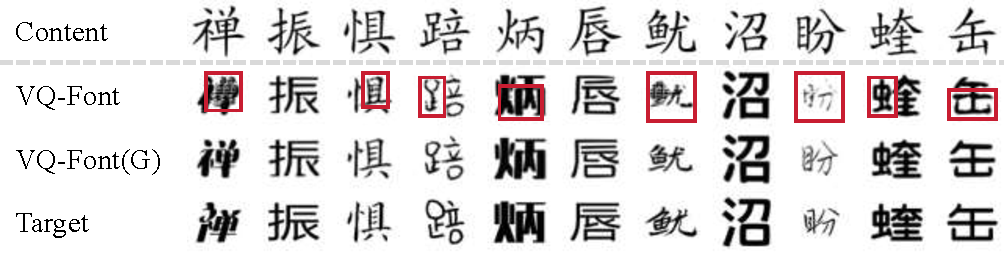
\includegraphics[width=0.95\linewidth]{SUPP_IMGS/EX_Visualization/VQ_G.pdf} 
  \caption{
Qualitative comparison on VQ-Font vs. VQ-Font (G). 
\textcolor{ex2figure_red}{\fbox{\rule{0pt}{4pt}\rule{4pt}{0pt}}} marks structural errors in the generated glyph. 
G-Tok improves structure preservation and produces more faithful font styles.
}
  \label{fig:supple_vq_g_ufuc}
\end{figure}


\begin{table*}[!t]
\centering
\caption{Quantitative evaluation of Multimodal FFG with full post-refinement (NFA and SE) on Unseen Fonts. All models listed are post-trained with NFA and SE stages on the Large dataset.}
\vspace{-2mm}
\setlength{\tabcolsep}{3pt}
\renewcommand{\arraystretch}{1.05}
\resizebox{0.95\textwidth}{!}{
\begin{tabular}{l | c c c c c c | c c c c c c }
\toprule
Method & \multicolumn{6}{c|}{Unseen Fonts Seen Characters (UFSC)} & \multicolumn{6}{c}{Unseen Fonts Unseen Characters (UFUC)} \\
\cmidrule(lr){2-7} \cmidrule(lr){8-13}
 & RMSE$\downarrow$ & SSIM$\uparrow$ & LPIPS$\downarrow$ & FID$\downarrow$ & Acc(C)$\uparrow$ & Acc(S)$\uparrow$
 & RMSE$\downarrow$ & SSIM$\uparrow$ & LPIPS$\downarrow$ & FID$\downarrow$ & Acc(C)$\uparrow$ & Acc(S)$\uparrow$ \\
\hline
$n_\text{ref}=2$ & 0.2501 & 0.6438 & 0.0888 & 10.1464 & \textbf{0.9851} & 0.3314 & 0.2701 & 0.5987 & 0.1069 & 9.4294 & 0.8720 & 0.3433 \\
$n_\text{ref}=4$ & 0.2437 & 0.6552 & 0.0848 & 9.5960  & 0.9839 & 0.3711 & 0.2692 & 0.6007 & 0.1049 & 9.0877 & 0.8828 & 0.3835 \\
$n_\text{ref}=8$ & 0.2398 & 0.6627 & 0.0831 & \textbf{8.3751}  & 0.9776 & 0.4154 & \textbf{0.2508} & \textbf{0.6377} & \textbf{0.0908} & \textbf{7.2034} & \textbf{0.9068} & 0.4183 \\
\Xhline{1.2pt}
GAR-Font($M_2$) & 0.2361 & 0.6707 & 0.0799 & 8.8867  & 0.9817 & 0.4508 & 0.2527 & 0.6352 & 0.0909 & 8.1444 & 0.9029 & 0.4247 \\
GAR-Font($M_4$) & \textbf{0.2358} & \textbf{0.6712} & \textbf{0.0796} & 8.8073  & 0.9800 & \textbf{0.4566} & 0.2524 & 0.6353 & \textbf{0.0908} & 8.0699 & 0.9023 & \textbf{0.4391} \\
\bottomrule
\end{tabular}
}
\label{tab:quant_eval_ref_mm}
\end{table*}
\begin{figure*}[!t]
    \centering
    \begin{minipage}{0.495\linewidth}
        \centering
        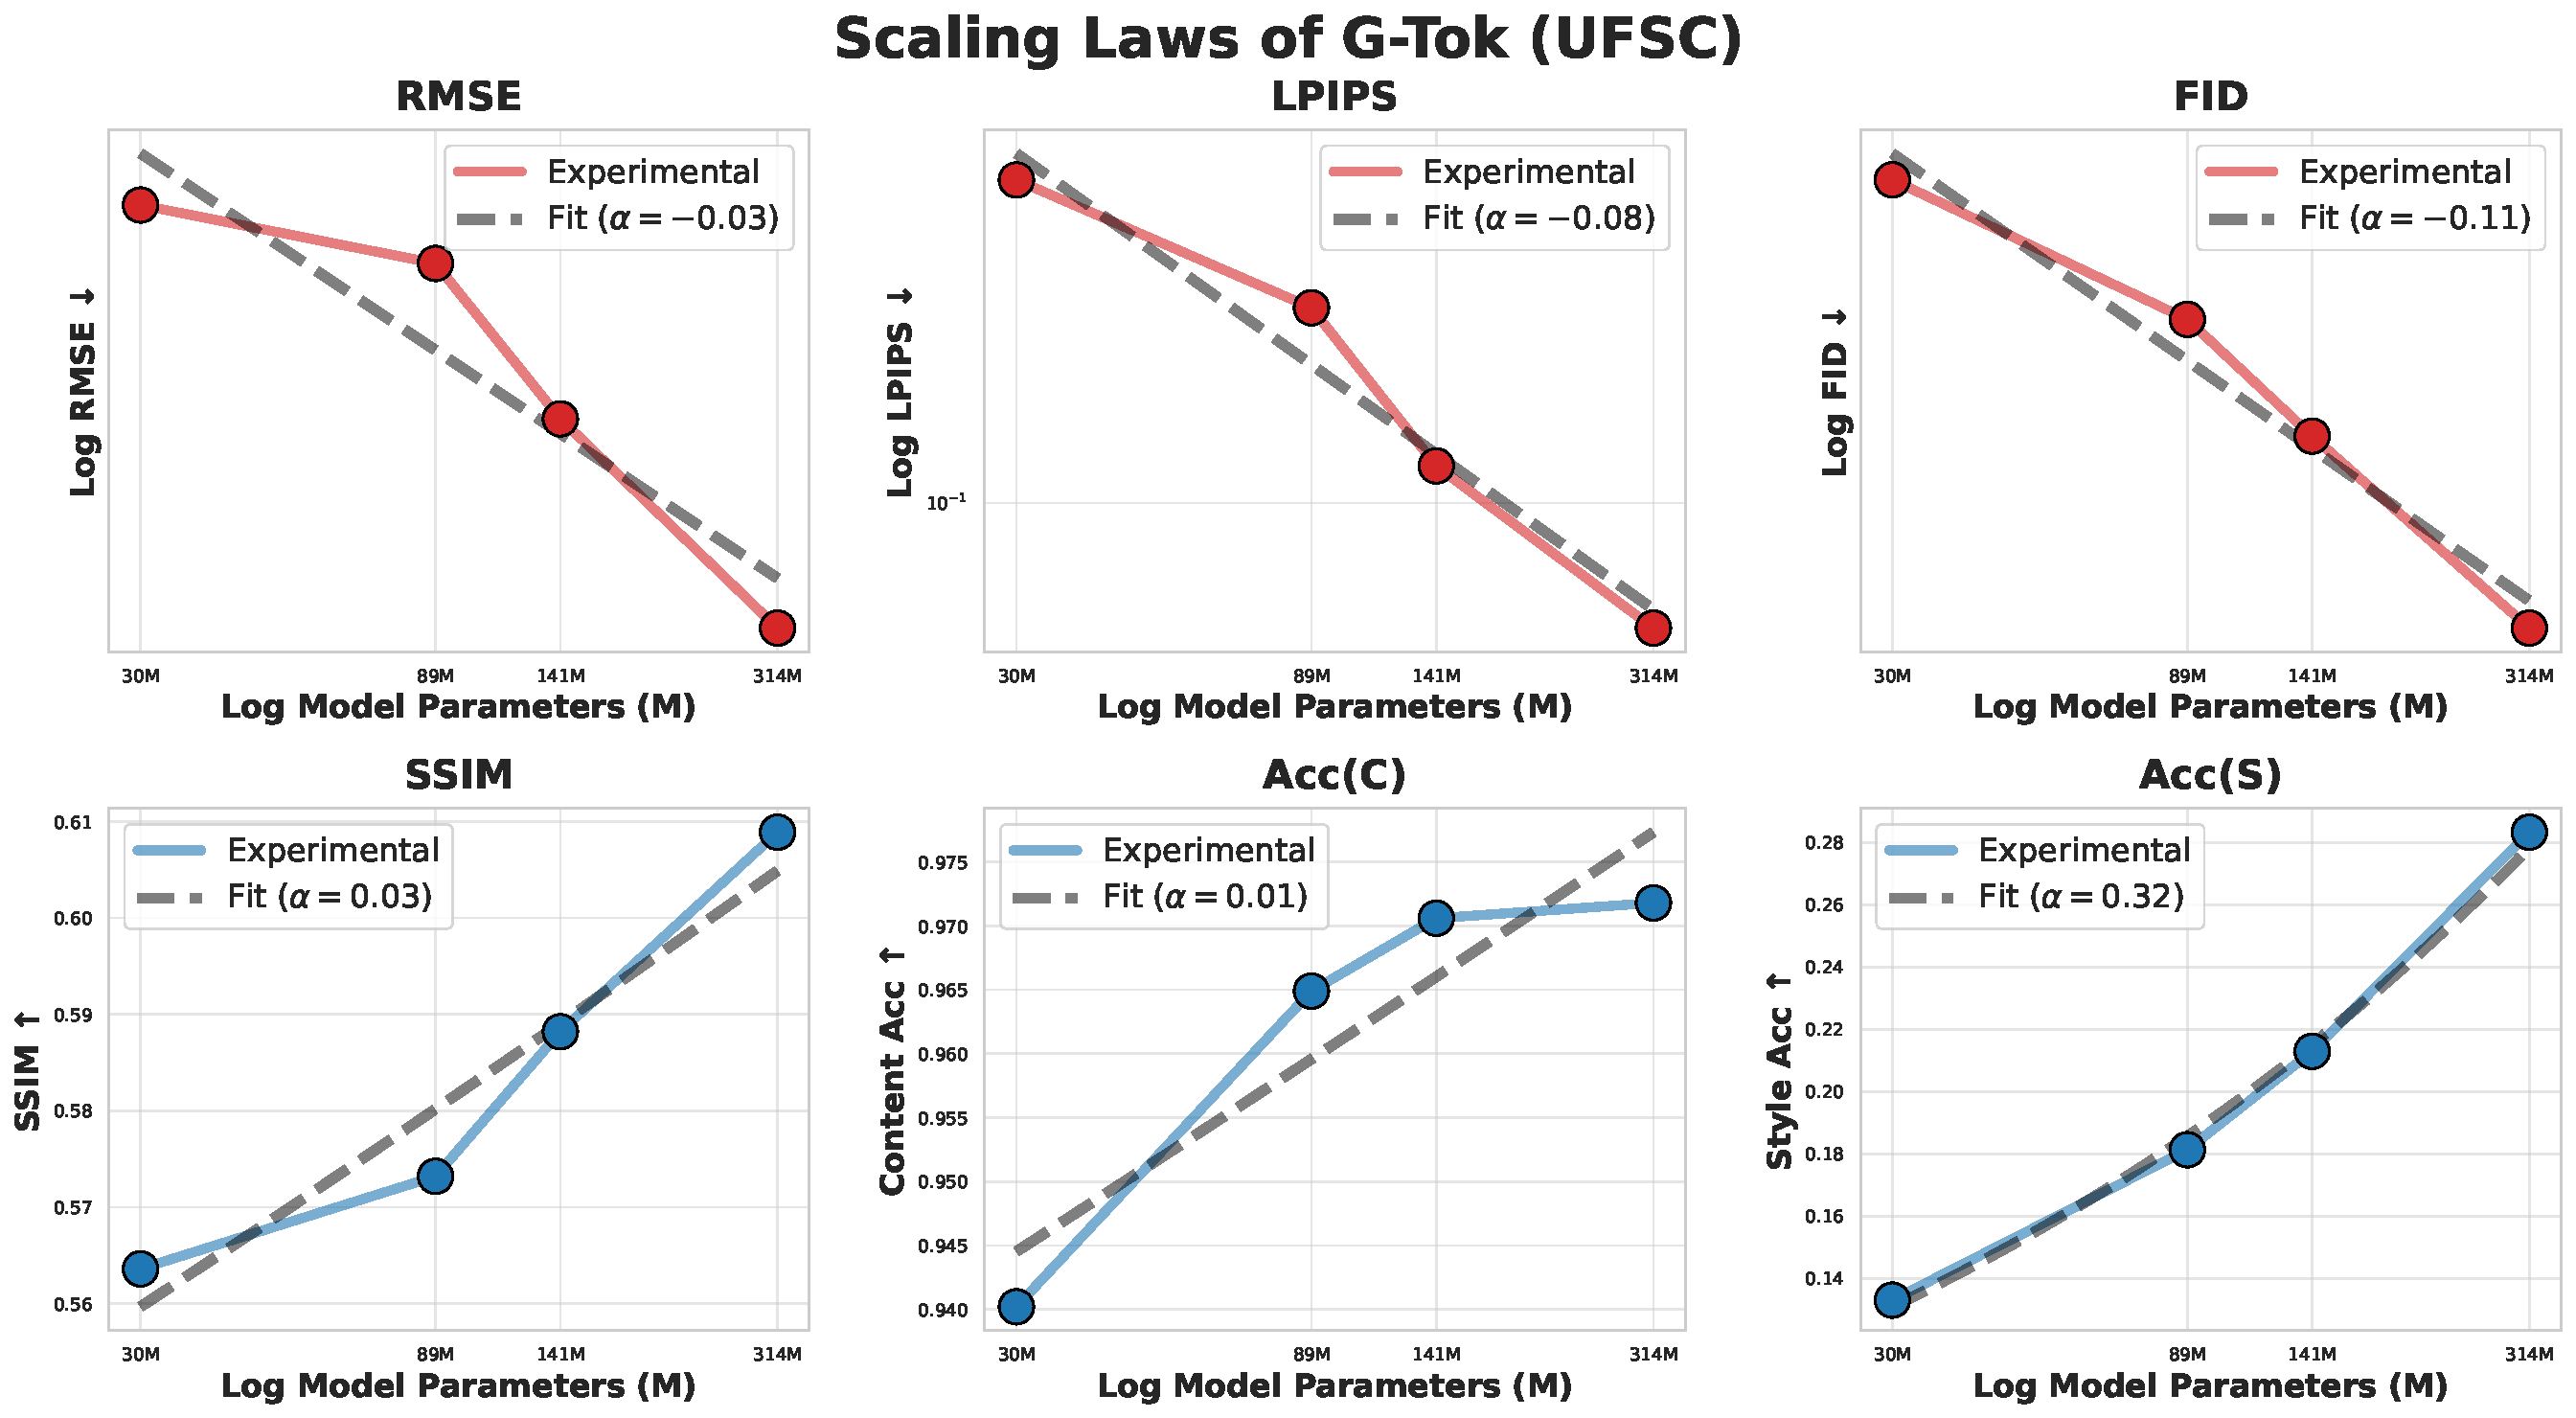
\includegraphics[width=\linewidth]{SUPP_IMGS/scaling_law_UFSC.pdf}
    \end{minipage}
    \hfill
    \begin{minipage}{0.495\linewidth}
        \centering
        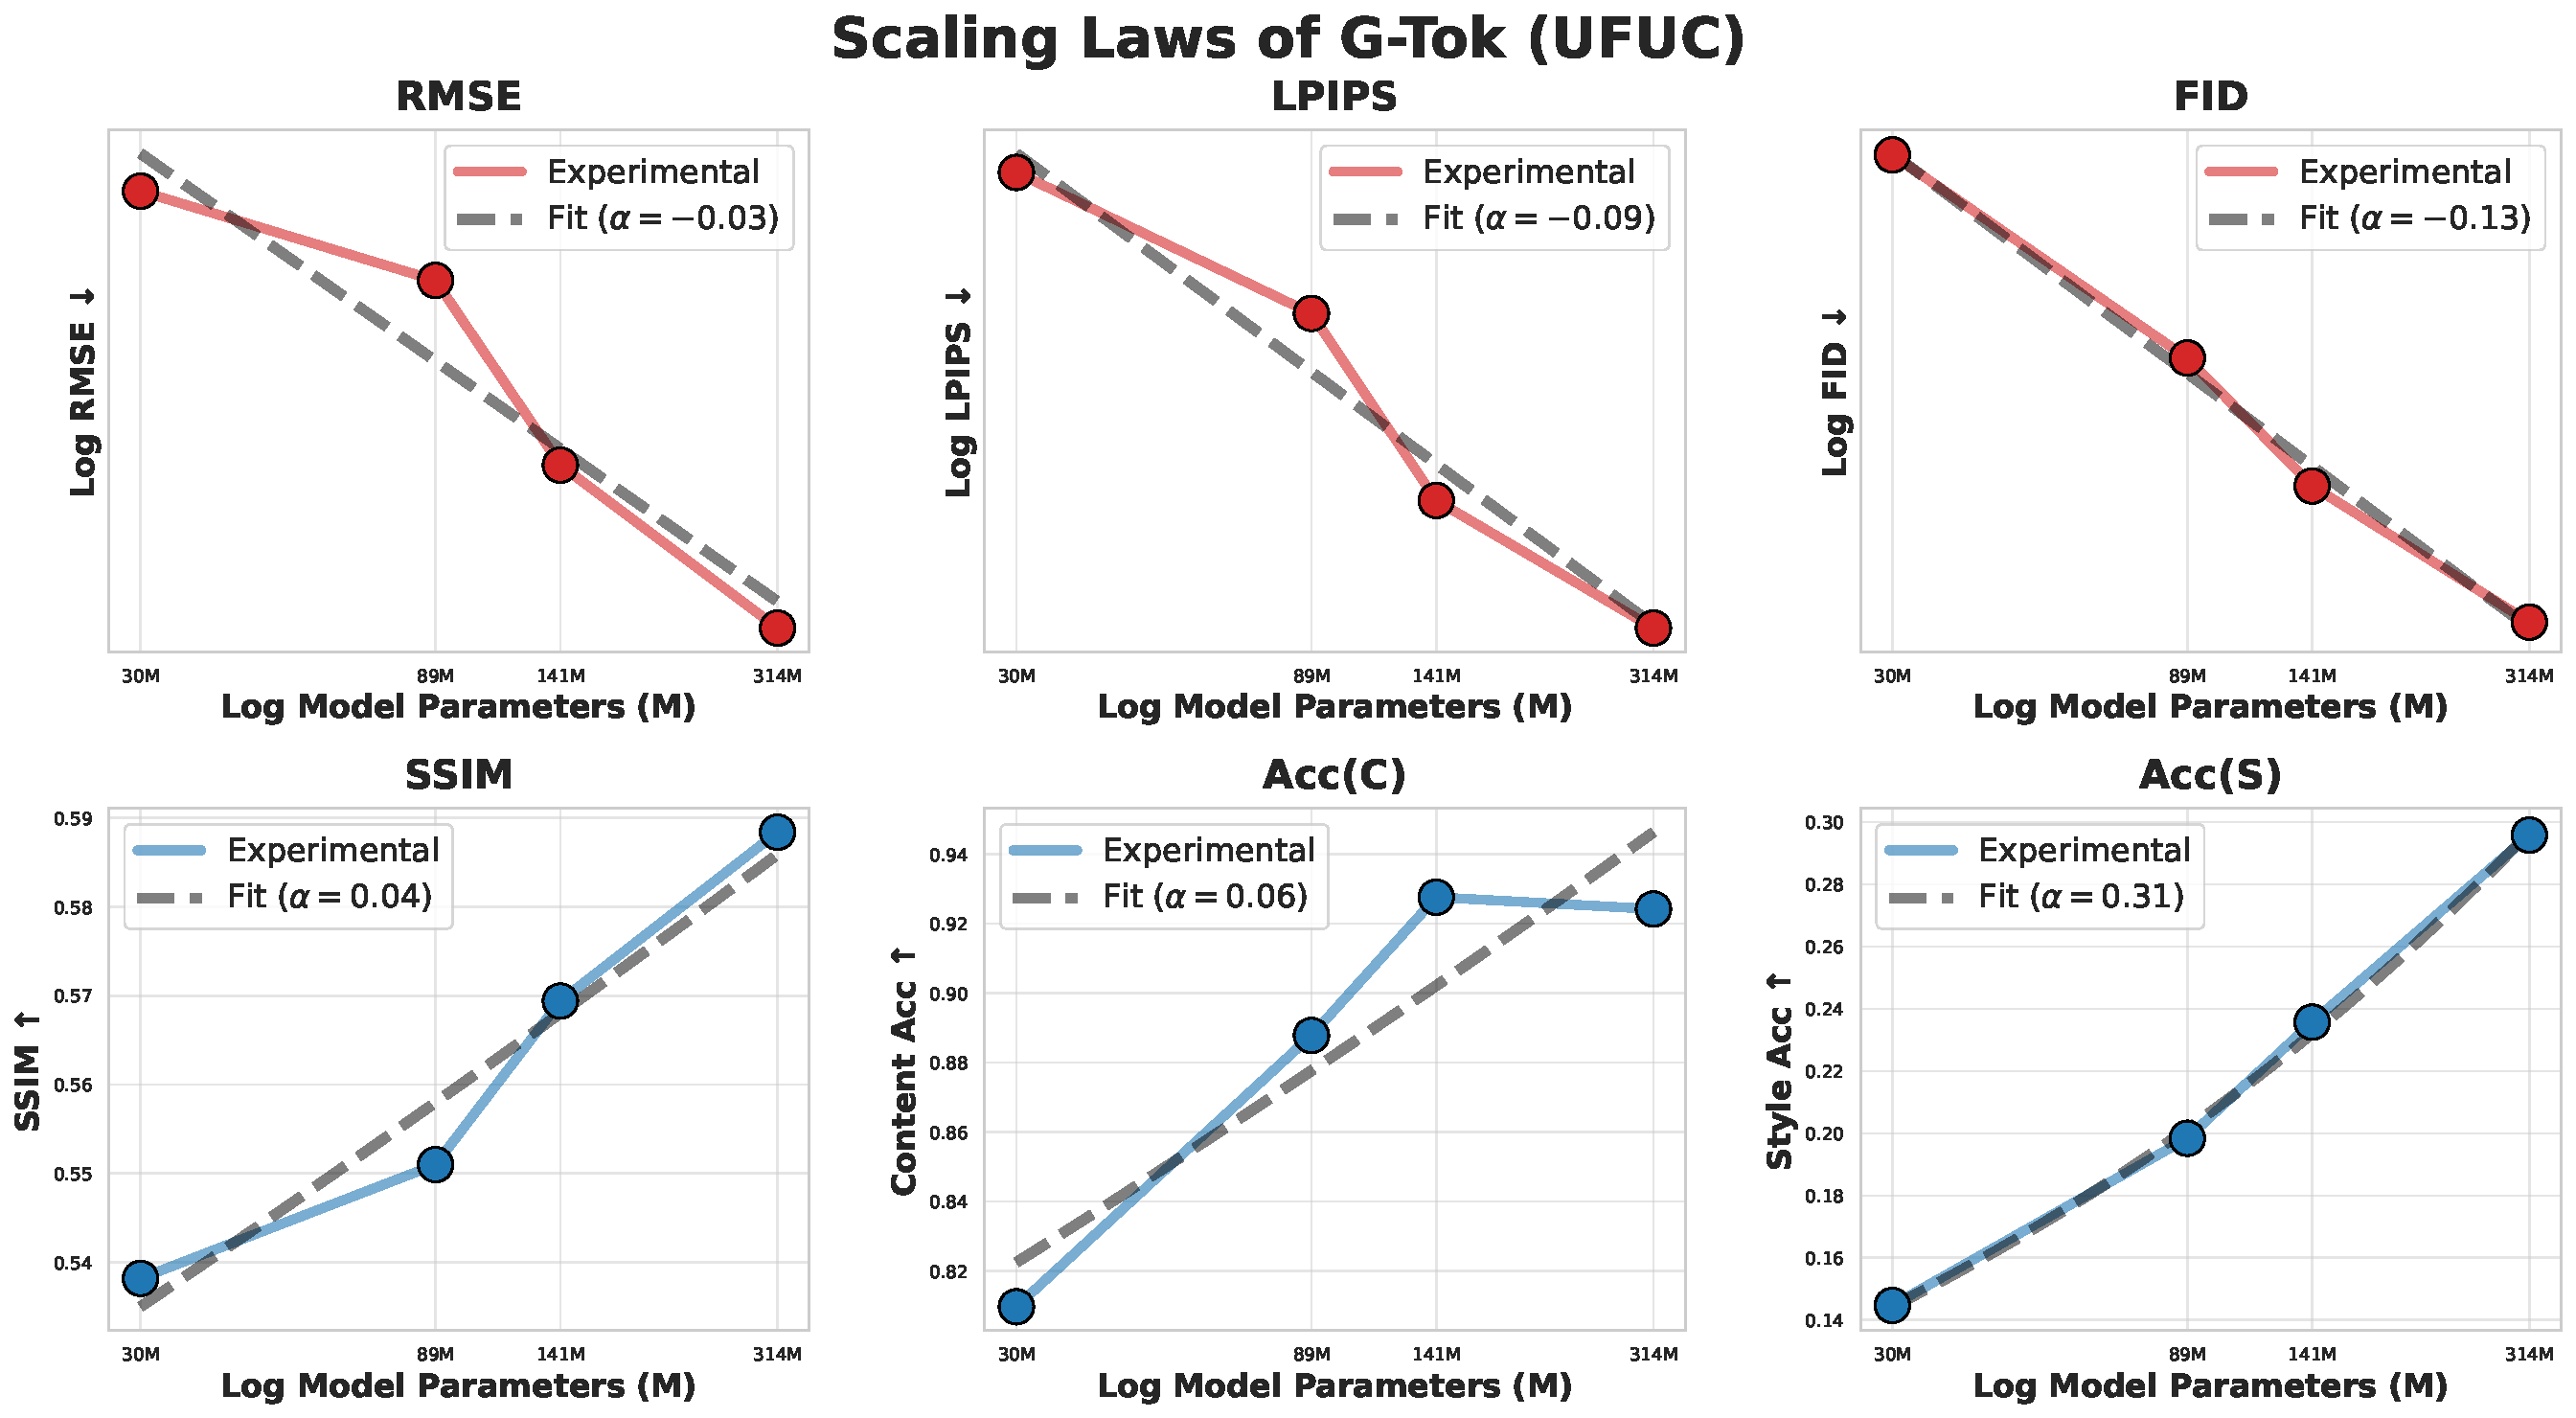
\includegraphics[width=\linewidth]{SUPP_IMGS/scaling_law_UFUC.pdf}
    \end{minipage}
    \vspace{-3mm}
    \caption{Scaling laws of the GAR-Font $(I_8)$ generator with NFA and SE refinement. The plots show performance metrics across model sizes (30M, 89M, 141M, 314M) on Unseen Fonts Seen Characters (\textit{UFSC}) and Unseen Fonts Unseen Characters (\textit{UFUC}). The dashed lines represent power-law fits, highlighting the predictable improvements in both perceptual quality and style generalization.}
    \vspace{-3mm}
    \label{fig:scaling_laws}
\end{figure*}
\subsection{Adaptation on G-Tok to Other FFG Methods}
\label{ssec:quantitiative_G-Tok_plugin}
To verify the versatility of our G-Tok, we integrated it into VQ-Font by replacing its native VQ-VAE with our G-Tok while maintaining the original model architecture and configuration. The modified model, \textbf{VQ-Font (G)}, was trained on the Small dataset with G-Tok. Due to time constraints, we trained it for only 150k iterations, compared with the 500k iterations used in the original VQ-Font. As shown in Table~\ref{tab:quant_eval_gtok_adaptation}, even under shorter training, this simple replacement yields significant improvements across all metrics. Most notably, FID$\downarrow$ decreases by nearly 50\% (e.g., $35.25 \to 17.33$ on \textit{UFSC}) and Content Accuracy$\uparrow$ improves by approximately 9\% ($\sim87\% \to \sim96\%$). These substantial gains demonstrate that G-Tok's hybrid CNN-ViT architecture captures far richer structural and stylistic semantics than standard VQ-VAEs, serving as a robust plug-and-play enhancement for quantization-based FFG methods. Figure~\ref{fig:supple_vq_g_ufuc} illustrates that integrating G-Tok helps the model preserve coherent global structures for complex fonts and generate styles that better align with the target font, indicating a richer and more semantically stable global representation G-Tok than the original VQ-VAE.


\subsection{Post-Refinement of Multimodal FFG}
\label{ssec:mm_post_refinement}

\begin{table*}[!t]
\centering
\caption{Quantitative evaluation of G-Tok's architecture on Unseen Fonts. All models listed are pre-trained on the Small dataset.}
\vspace{-2mm}
\setlength{\tabcolsep}{3pt}
\renewcommand{\arraystretch}{1.05}
\resizebox{0.95\textwidth}{!}{
\begin{tabular}{l | c c c c c c | c c c c c c }
\toprule
Method & \multicolumn{6}{c|}{Unseen Fonts Seen Characters (UFSC)} & \multicolumn{6}{c}{Unseen Fonts Unseen Characters (UFUC)} \\
\cmidrule(lr){2-7} \cmidrule(lr){8-13}
 & RMSE$\downarrow$ & SSIM$\uparrow$ & LPIPS$\downarrow$ & FID$\downarrow$ & Acc(C)$\uparrow$ & Acc(S)$\uparrow$ 
 & RMSE$\downarrow$ & SSIM$\uparrow$ & LPIPS$\downarrow$ & FID$\downarrow$ & Acc(C)$\uparrow$ & Acc(S)$\uparrow$ \\
\hline
CNN & 0.3212 & 0.4836 & 0.1442 & 9.5071 & 0.9051 & 0.0235 & 0.3447 & 0.4350 & 0.1728 & 10.5239 & 0.6722 & 0.0221 \\
CNN+Non-Causal ViT & 0.3183 & 0.4919 & 0.1458 & \textbf{7.9101} & 0.9268 & 0.0402 & 0.3271 & 0.4745 & 0.1562 & 8.7504 & 0.8019 & 0.0436 \\
CNN+Causal ViT & \textbf{0.3080} & \textbf{0.5052} & \textbf{0.1313} & 7.9484 & \textbf{0.9408} & \textbf{0.0802} & \textbf{0.3142} & \textbf{0.4932} & \textbf{0.1421} & \textbf{8.4841} & \textbf{0.8993} & \textbf{0.0796} \\
\bottomrule
\end{tabular}
}
\label{tab:ablation_gtok_generator}
\end{table*}

In Section 4.4, we demonstrated the efficacy of G-Tok$(M_2/M_4)$ on multimodal FFG, but limited to pretraining stage. To fully assess the potential of our lightweight vision-language adaptation, we extend the evaluation to the complete pipeline. We apply our post-training NFA and SE stages to both the vision-only baselines and our multimodal variants. All models are trained on the Large (\textit{L}) dataset.

As visualized in Table~\ref{tab:quant_eval_ref_mm}, the inclusion of textual descriptions significantly enhances the effectiveness of the post-refinement stage. Unlike the pre-training phase where multimodal models showed a slight dip in style accuracy (Acc(S)$\uparrow$), the fully refined GAR-Font($M_2$) and GAR-Font($M_4$) exhibit a substantial lead in Acc(S)$\uparrow$ compared to their vision-only counterparts ($n_\text{ref}=2$ and $n_\text{ref}=4$). Notably, \textbf{GAR-Font($M_4$) outperforms the 8-reference vision-only baseline ($n_\text{ref}=8$)} across most key metrics, including RMSE$\downarrow$, SSIM$\uparrow$, LPIPS$\downarrow$, and Style Accuracy$\uparrow$ (0.4566 vs. 0.4154 on \textit{UFSC}).


\subsection{Scaling Laws of GAR-Font\texorpdfstring{$(I_8)$}{(I8)}}
\label{ssec:scaling_law}
We evaluate the scalability of GAR-Font$(I_8)$ with NFA and SE on the small dataset by training models from 30M to 314M parameters and measuring performance across standard quantitative metrics. Following established scaling-law formulations, we model the relationship between model size $N$ and loss metric $L$ using a power law $L(N)\propto N^{-\alpha}$, and analyze trends in log–log space, where an ideal scaling law appears linear and the slope $\alpha$ reflects scaling efficiency.

As shown in Figure~\ref{fig:scaling_laws}, the enhanced GAR-Font models closely follow these power-law predictions, exhibiting smooth, monotonic improvements across all metrics. Loss-based metrics (FID$\downarrow$, LPIPS$\downarrow$, RMSE$\downarrow$) scale linearly with negative slopes, with FID$\downarrow$ showing a pronounced gain, indicating that larger models continue to yield substantial perceptual improvements without saturation. Accuracy metrics display complementary behavior: Content Accuracy (Acc(C)$\uparrow$) saturates early due to task simplicity, whereas Style Accuracy (Acc(S)$\uparrow$) benefits most from increased capacity. This steep scaling trend highlights that NFA and SE effectively exploit larger parameter budgets to capture and generalize complex stylistic attributes, underscoring the central role of scale in high-fidelity font generation.





% \subsection{Post-Refinement of GAR-Font\texorpdfstring{$(M_2/M_4)$}{(M2/M4)}}

% To fully explore the potential of our lightweight language-style adaptation, we apply the complete post-refinement pipeline (NFA and SE) to GAR-Font($M_2$) and GAR-Font($M_4$). 

% \begin{table*}[t]
% \centering
% \caption{Quantitative evaluation on unseen fonts (MM Post-Refinement train on Large).}
% \vspace{-2mm}
% \setlength{\tabcolsep}{3pt}
% \renewcommand{\arraystretch}{1.05}
% \resizebox{0.95\textwidth}{!}{
% \begin{tabular}{l | c c c c c c | c c c c c c }
% \toprule
% Method & \multicolumn{6}{c|}{Unseen Fonts Seen Characters (UFSC)} & \multicolumn{6}{c}{Unseen Fonts Unseen Characters (UFUC)} \\
% \cmidrule(lr){2-7} \cmidrule(lr){8-13}
%  & RMSE$\downarrow$ & SSIM$\uparrow$ & LPIPS$\downarrow$ & FID$\downarrow$ & Acc(C)$\uparrow$ & Acc(S)$\uparrow$
%  & RMSE$\downarrow$ & SSIM$\uparrow$ & LPIPS$\downarrow$ & FID$\downarrow$ & Acc(C)$\uparrow$ & Acc(S)$\uparrow$ \\
% \hline
% I8\_NFA\_SE\_ref2   & 0.2501 & 0.6438 & 0.0888 & 10.1464 & \textbf{0.9851} & 0.3314 & 0.2701 & 0.5987 & 0.1069 & 9.4294 & 0.8720 & 0.3433 \\
% I8\_NFA\_SE\_ref4   & 0.2437 & 0.6552 & 0.0848 & 9.5960  & 0.9839 & 0.3711 & 0.2692 & 0.6007 & 0.1049 & 9.0877 & 0.8828 & 0.3835 \\
% I8\_NFA\_SE\_ref8   & 0.2398 & 0.6627 & 0.0831 & \textbf{8.3751}  & 0.9776 & 0.4154 & \textbf{0.2508} & \textbf{0.6377} & \textbf{0.0908} & \textbf{7.2034} & \textbf{0.9068} & 0.4183 \\
% MM2\_NFA\_SE        & 0.2361 & 0.6707 & 0.0799 & 8.8867  & 0.9817 & 0.4508 & 0.2527 & 0.6352 & 0.0909 & 8.1444 & 0.9029 & 0.4247 \\
% MM4\_NFA\_SE        & \textbf{0.2358} & \textbf{0.6712} & \textbf{0.0796} & 8.8073  & 0.9800 & \textbf{0.4566} & 0.2524 & 0.6353 & 0.0908 & 8.0699 & 0.9023 & \textbf{0.4391} \\
% \bottomrule
% \end{tabular}
% }
% \label{tab:quant_eval_ref_mm}
% \end{table*}
% \begin{table*}[t]
% \centering
% \caption{Quantitative evaluation on unseen fonts (VQ-Font vs VQ-Font (G).}
% \vspace{-2mm}
% \setlength{\tabcolsep}{3pt}
% \renewcommand{\arraystretch}{1.05}
% \resizebox{0.95\textwidth}{!}{
% \begin{tabular}{l | c c c c c c | c c c c c c }
% \toprule
% Method & \multicolumn{6}{c|}{Unseen Fonts Seen Characters (UFSC)} & \multicolumn{6}{c}{Unseen Fonts Unseen Characters (UFUC)} \\
% \cmidrule(lr){2-7} \cmidrule(lr){8-13}
%  & RMSE$\downarrow$ & SSIM$\uparrow$ & LPIPS$\downarrow$ & FID$\downarrow$ & Acc(C)$\uparrow$ & Acc(S)$\uparrow$
%  & RMSE$\downarrow$ & SSIM$\uparrow$ & LPIPS$\downarrow$ & FID$\downarrow$ & Acc(C)$\uparrow$ & Acc(S)$\uparrow$ \\
% \hline
% VQ\_Font & 0.2727 & 0.5642 & 0.1830 & 35.2472 & 0.8763 & 0.0016 & 0.2744 & 0.5616 & 0.1822 & 36.7914 & 0.8882 & 0.0016 \\
% VQ\_Font (G)   & 0.2725 & 0.5644 & 0.1731 & 17.3296  & 0.9646 & 0.0022 & - & - & - & - &- &- \\
% \bottomrule
% \end{tabular}
% }
% \label{tab:quant_eval_ref_mm}
% \end{table*}


% \subsection{Scaling Laws of GAR-Font$(I_8)$}
% 340M, 150M, 90M, 50M
% To explore how model capacity affects autoregressive font generation, we conduct an additional scaling study on the AR Generator using the Small dataset. We train models of varying sizes and evaluate them across the full set of quantitative metrics, reported in Table~S\_X. The results show a consistent monotonic improvement with increasing model size, demonstrating a clear scaling trend for AR-based glyph modeling.
% \begin{table*}[t]
% \centering
% \caption{Quantitative evaluation on unseen fonts. (Scaling Law, Train on Small)}
% \vspace{-2mm}
% \setlength{\tabcolsep}{3pt}
% \renewcommand{\arraystretch}{1.05}
% \resizebox{0.95\textwidth}{!}{
% \begin{tabular}{l | c c c c c c | c c c c c c }
% \toprule
% Method & \multicolumn{6}{c|}{Unseen Fonts Seen Characters (UFSC)} & \multicolumn{6}{c}{Unseen Fonts Unseen Characters (UFUC)} \\
% \cmidrule(lr){2-7} \cmidrule(lr){8-13}
%  & RMSE$\downarrow$ & SSIM$\uparrow$ & LPIPS$\downarrow$ & FID$\downarrow$ & Acc(C)$\uparrow$ & Acc(S)$\uparrow$
%  & RMSE$\downarrow$ & SSIM$\uparrow$ & LPIPS$\downarrow$ & FID$\downarrow$ & Acc(C)$\uparrow$ & Acc(S)$\uparrow$ \\
% \hline
% 50M\_Pre & 0.3234 & 0.4803 & 0.1478 & 9.5682 & 0.9002 & 0.0347 & 0.3233 & 0.4826 & 0.1473 & 9.8740 & 0.8878 & 0.0375 \\
% 90M\_Pre & 0.3219 & 0.4879 & 0.1409 & 7.9230 & 0.9220 & 0.0448 & 0.3212 & 0.4911 & 0.1409 & 8.1393 & 0.9094 & 0.0502 \\
% 150M\_Pre & 0.3212 & 0.4845 & 0.1449 & 7.9945 & 0.9297 & 0.0471 & 0.3210 & 0.4864 & 0.1449 & 8.4493 & 0.9281 & 0.0506 \\
% 340M\_Pre & 0.3080 & 0.5052 & 0.1313 & 7.9484 & 0.9408 & 0.0802 & 0.3142 & 0.4932 & 0.1421 & 8.4841 & 0.8993 & 0.0796 \\
% \hline
% 50M\_NFA & 0.2977 & 0.5280 & 0.1241 & 10.0811 & 0.7837 & 0.1026 & 0.2979 & 0.5293 & 0.1235 & 10.2685 & 0.7455 & 0.1234 \\
% 90M\_NFA & 0.2937 & 0.5404 & 0.1172 & 7.7879 & 0.8371 & 0.1549 & 0.2928 & 0.5441 & 0.1164 & 7.8355 & 0.8124 & 0.1766 \\
% 150M\_NFA & 0.2874 & 0.5563 & 0.1107 & 6.5190 & 0.8599 & 0.2009 & 0.2862 & 0.5602 & 0.1094 & 6.7234 & 0.8448 & 0.2208 \\
% 340M\_NFA & 0.2712 & 0.5933 & 0.0992 & \textbf{5.4254} & 0.9236 & \textbf{0.3179} & 0.2836 & 0.5702 & 0.1079 & \textbf{5.6667} & 0.8817 & \textbf{0.3277} \\
% \hline
% 50M\_NFA\_SE & 0.2854 & 0.5636 & 0.1148 & 8.9481 & 0.9402 & 0.1330 & 0.2988 & 0.5382 & 0.1257 & 9.6713 & 0.8097 & 0.1447 \\
% 90M\_NFA\_SE & 0.2828 & 0.5732 & 0.1087 & 8.2565 & 0.9649 & 0.1813 & 0.2946 & 0.5510 & 0.1179 & 8.4715 & 0.8878 & 0.1984 \\
% 150M\_NFA\_SE & 0.2760 & 0.5882 & 0.1016 & 7.7190 & 0.9706 & 0.2129 & 0.2861 & 0.5694 & 0.1083 & 7.7930 & 0.9276 & 0.2357 \\
% 340M\_NFA\_SE & \textbf{0.2671} & \textbf{0.6089} & \textbf{0.0948} & 6.9103 & \textbf{0.9718} & 0.2833 & \textbf{0.2788} & \textbf{0.5884} & \textbf{0.1022} & 7.1309 & \textbf{0.9242} & 0.2958 \\
% \bottomrule
% \end{tabular}
% }
% \label{tab:quant_eval_fonts}
% \end{table*}



\section{Additional Ablative Studies}
\label{sec:Ablate}
\subsection{On G-Tok's hybrid Architecture}
% Reconstruction results (0.2 0.2)
To further illustrate the robustness of our hybrid CNN–ViT tokenizer, we provide complete visualizations of the \textbf{Reconstruction Robustness} experiment, where glyphs are corrupted with localized Gaussian noise ($\sigma = 0.2$, affecting 20\% area).  
The qualitative results in Figure~\ref{fig:supple_abl1_rec} demonstrate that G-Tok robustly recovers structural layout and stylistic traits even under severe perturbations, while non-hybrid alternatives fail to reconstruct consistent structure. 

% This visual evidence complements the quantitative robustness results in Section~5.3.

\subsection{On G-Tok's Global and Causal Modeling}
% UFSC,  UFUC,  Small dataset
We present full ablation results for the global and causal modeling components of G-Tok.  
Table ~\ref{tab:ablation_gtok_generator} reports the complete quantitative comparison on the \textit{UFSC/UFUC}. As discussed in Section~5.3, adding global self-attention (CNN + Non-causal ViT) significantly outperforms the CNN-only baseline, while the causal ViT further improves sequential modeling and yields the best overall performance.


Figure ~\ref{fig: supple_abl2_all} provides qualitative comparisons on (\textit{UFSC}, Small) and (\textit{UFUC}, Small). The AR Generator implemented with a CNN-only tokenizer often exhibits style mismatches and inconsistent strokes. Introducing ViT modules into the tokenizer enhances its ability to perceive and capture global stylistic context, leading to more coherent font generation. The AR variant with full G-Tok (CNN + Causal ViT) achieves the most robust performance, showing visible improvements in stylistic and  structural fidelity.

\subsection{On AR Generator's Soft-Decoding}
We provide full visualizations to assess the impact of pixel-level supervision and the soft-decoding strategy. As shown in Figure~\ref{fig: supple_abl3_all} under both (\textit{UFSC}, Small) and (\textit{UFUC}, Small), pixel-level supervision enhances structural accuracy, while soft decoding yields smoother, more continuous strokes and reduces broken segments and visual artifacts.



\begin{figure}[t]
  \centering
  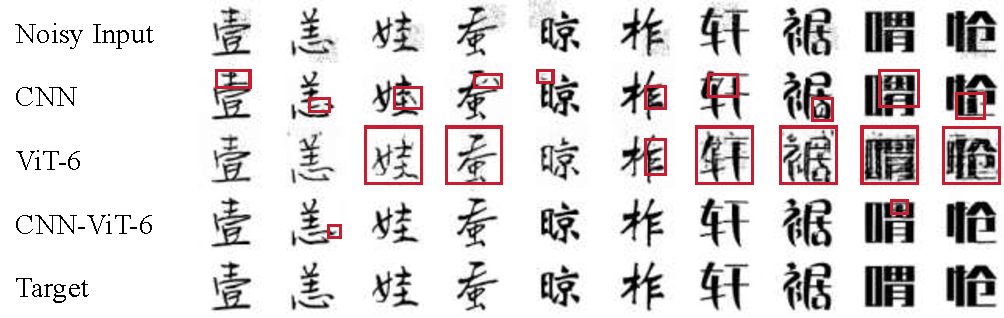
\includegraphics[width=0.95\linewidth]{SUPP_IMGS/EX_Visualization/ABL1_Rec.pdf} 
  \vspace{-3mm}
  \caption{Reconstruction Robustness under localized Gaussian noise ($\sigma = 0.2$, 20\% area). \textcolor{ex2figure_red}{\fbox{\rule{0pt}{4pt}\rule{4pt}{0pt}}} marks structural mistakes. G-Tok maintains structural and stylistic fidelity despite heavy corruption, while non-hybrid tokenizers exhibit unstable and inconsistent reconstructions.}
  \vspace{-3mm}
  \label{fig:supple_abl1_rec}
\end{figure}

\begin{figure*}[tp] % [p] 强制将这些内容放在单独的一页
    \centering
    
    % ================== 第一组图 (G-Tok) ==================
    \begin{subfigure}{0.93\linewidth} % 尝试缩小到 0.8 或 0.75
        \centering
        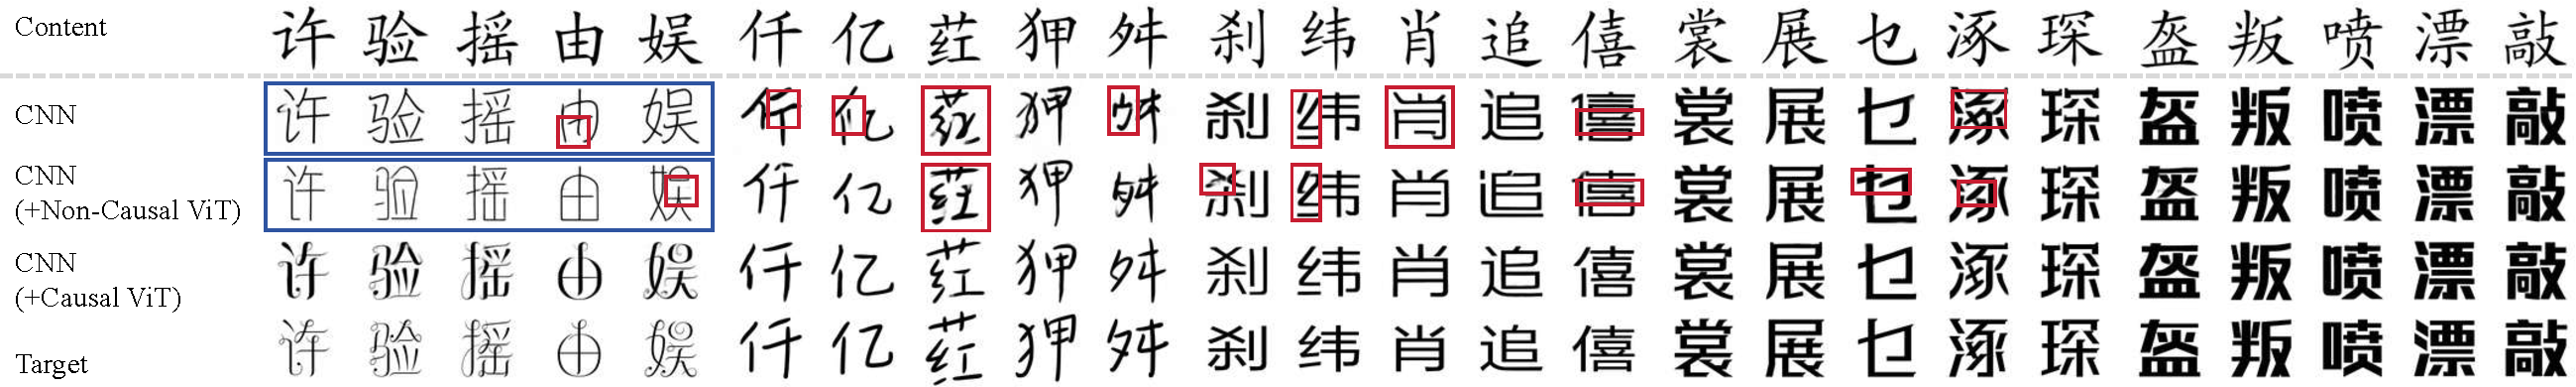
\includegraphics[width=\linewidth]{SUPP_IMGS/EX_Visualization/ABL2_table_UFSC_Small.pdf}
        \caption{\textit{UFSC}, Small dataset}
        \label{fig: supple_abl2_ufsc_small}
    \end{subfigure}
    \\ % 强制换行，确保垂直排列
    \begin{subfigure}{0.93\linewidth}
        \centering
        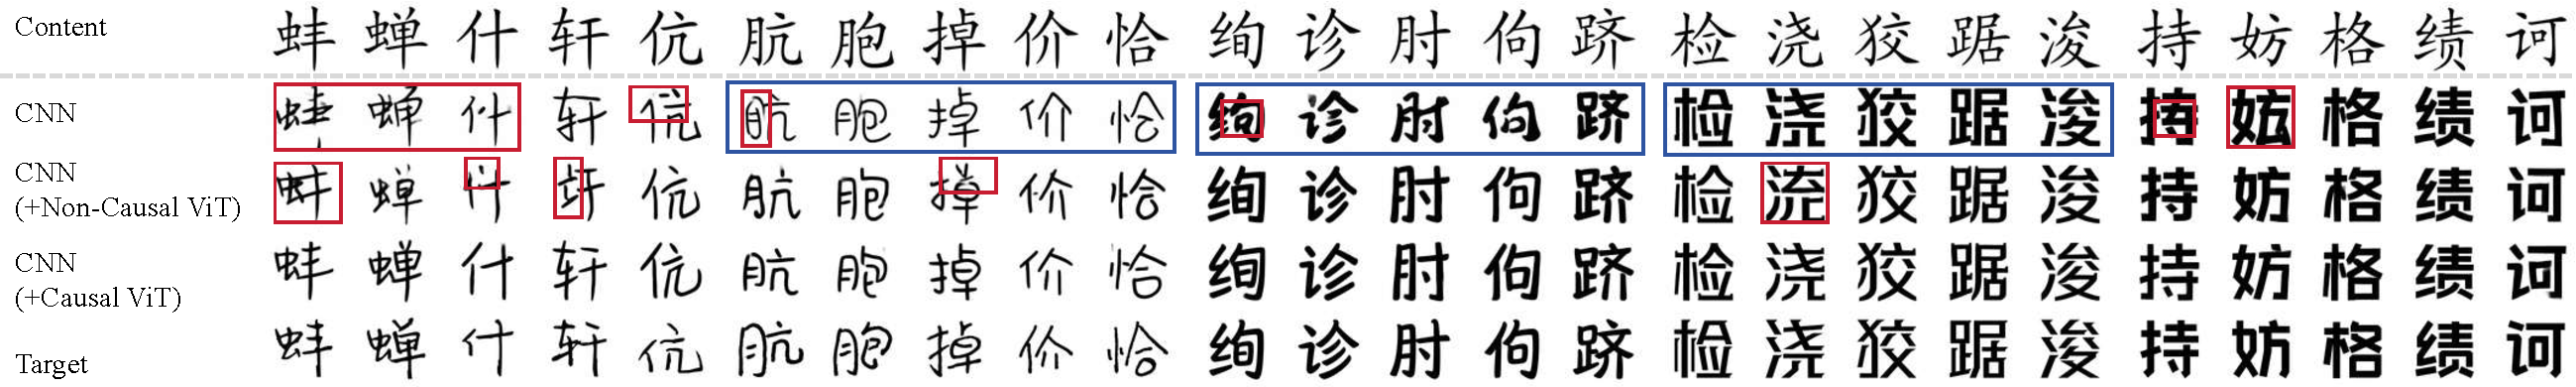
\includegraphics[width=\linewidth]{SUPP_IMGS/EX_Visualization/ABL2_table_UFUC_Small.pdf}
        \caption{\textit{UFUC}, Small dataset}
        \label{fig: supple_abl2_ufuc_small}
    \end{subfigure}
    \vspace{-3mm}
    \caption{Qualitative results on G-Tok's Global and Causal Modeling under \textit{UFSC} and \textit{UFUC} protocols
        (Small dataset). 
        \textcolor{ex1figure_red}{\fbox{\rule{0pt}{4pt}\rule{4pt}{0pt}}} /
        \textcolor{ex1figure_blue}{\fbox{\rule{0pt}{4pt}\rule{4pt}{0pt}}}
        indicate structural errors and style mismatches.}
    \label{fig: supple_abl2_all}
    
    \vspace{1em} % 在不同 Figure 之间增加一点区分距离
    
    % ================== 第二组图 (AR Generator) ==================
    \begin{subfigure}{0.93\linewidth}
        \centering
        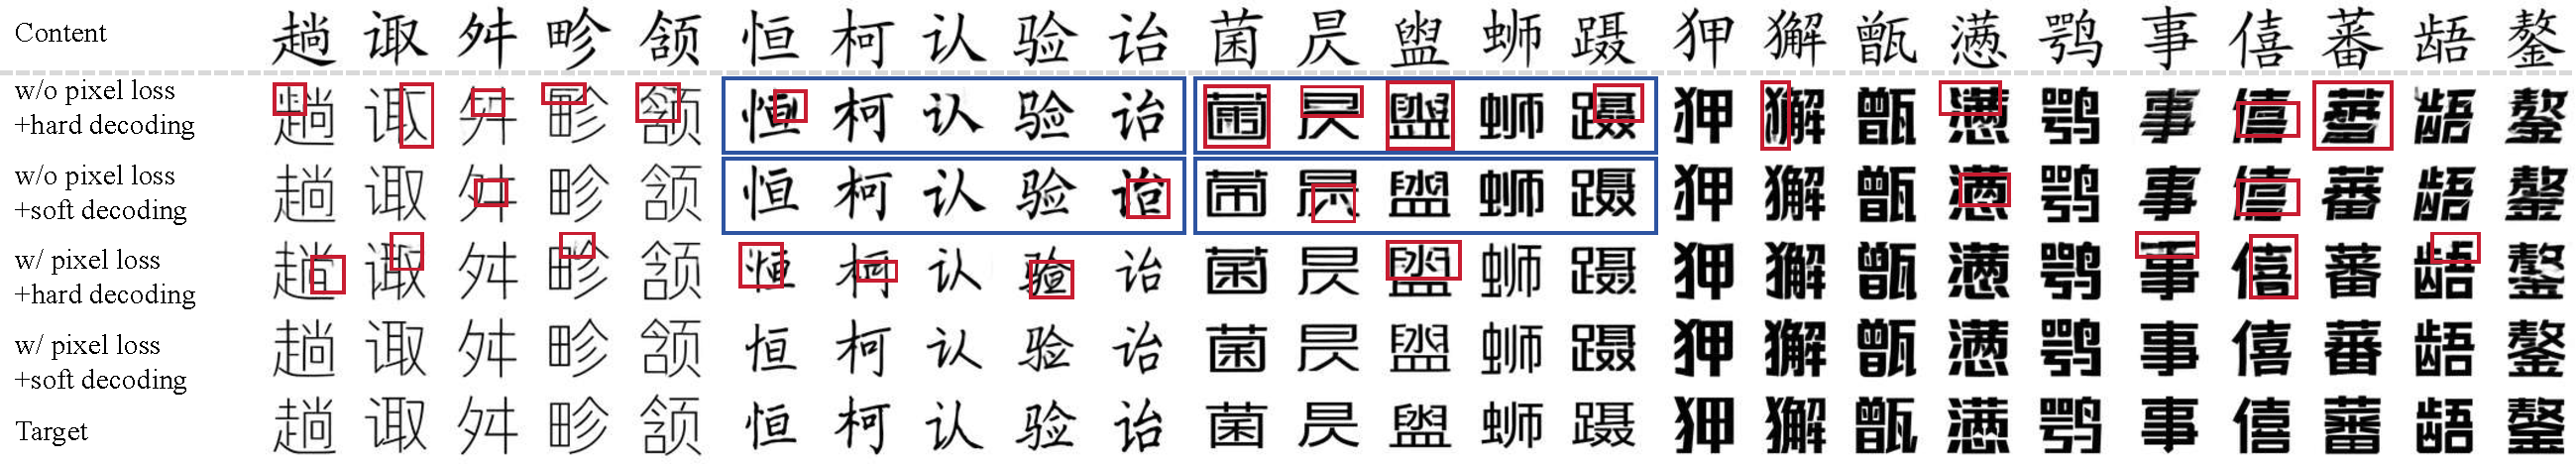
\includegraphics[width=\linewidth]{SUPP_IMGS/EX_Visualization/ABL3_Table_UFSC_Small.pdf}
        \caption{\textit{UFSC}, Small dataset}
        \label{fig: supple_abl3_ufsc_small}
    \end{subfigure}
    \\
    \begin{subfigure}{0.93\linewidth}
        \centering
        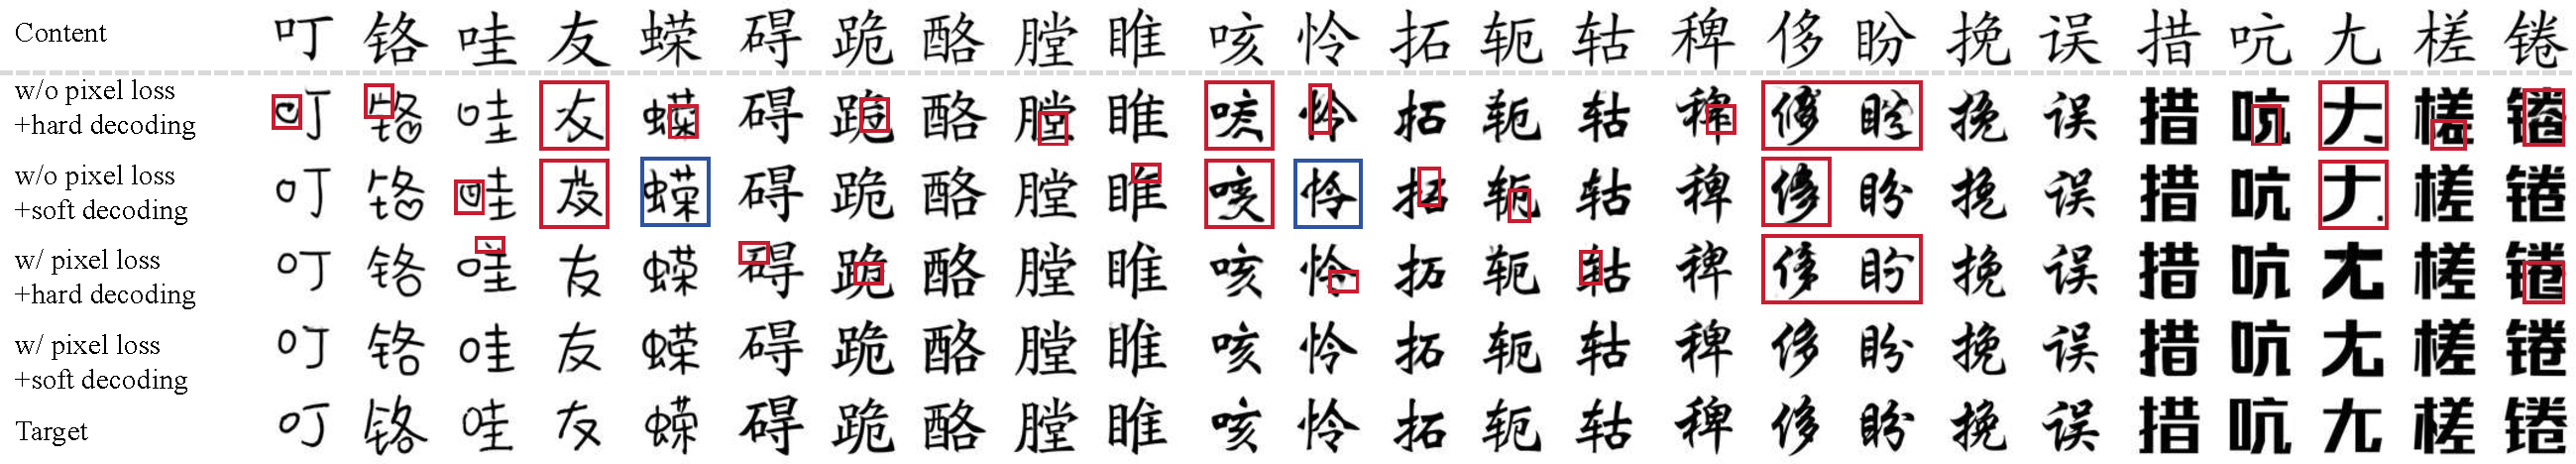
\includegraphics[width=\linewidth]{SUPP_IMGS/EX_Visualization/ABL3_Table_UFUC_Small.pdf}
        \caption{\textit{UFUC}, Small dataset}
        \label{fig: supple_abl3_ufuc_small}
    \end{subfigure}
    \vspace{-3mm}
    \caption{Qualitative results on AR Generator's Soft-decoding under \textit{UFSC} and \textit{UFUC} protocols
        (Small dataset).
        \textcolor{ex1figure_red}{\fbox{\rule{0pt}{4pt}\rule{4pt}{0pt}}} /
        \textcolor{ex1figure_blue}{\fbox{\rule{0pt}{4pt}\rule{4pt}{0pt}}}
        indicate structural errors and style mismatches.}
    \label{fig: supple_abl3_all}

    \vspace{1em}

    % ================== 第三组图 (Multimodal Style) ==================
    \begin{subfigure}{0.93\linewidth}
        \centering
        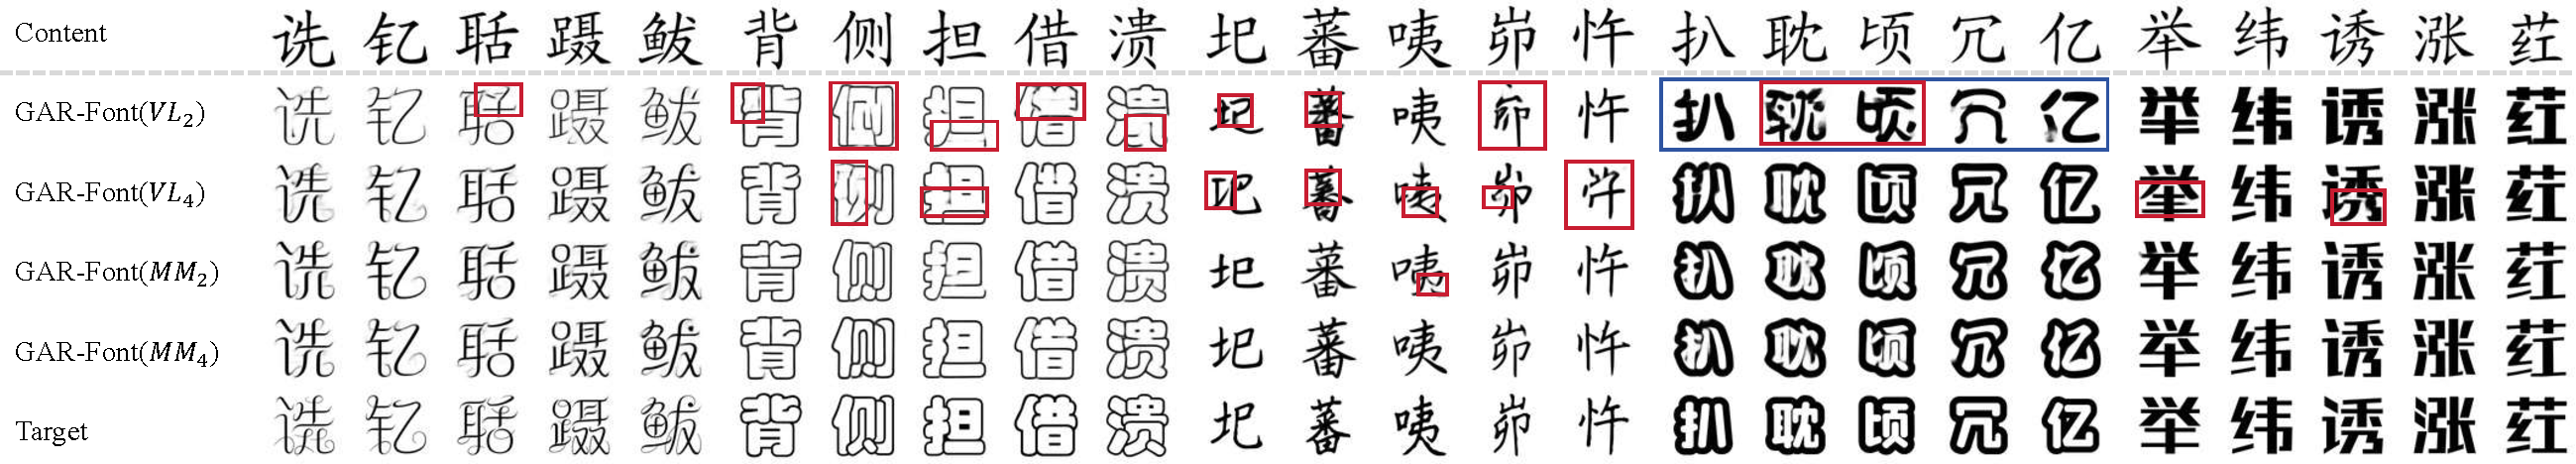
\includegraphics[width=\linewidth]{SUPP_IMGS/EX_Visualization/ABL4_Table_UFSC_Large.pdf}
        \caption{\textit{UFSC}, Large dataset}
        \label{fig: supple_abl4_ufsc_large}
    \end{subfigure}
    \\
    \begin{subfigure}{0.93\linewidth}
        \centering
        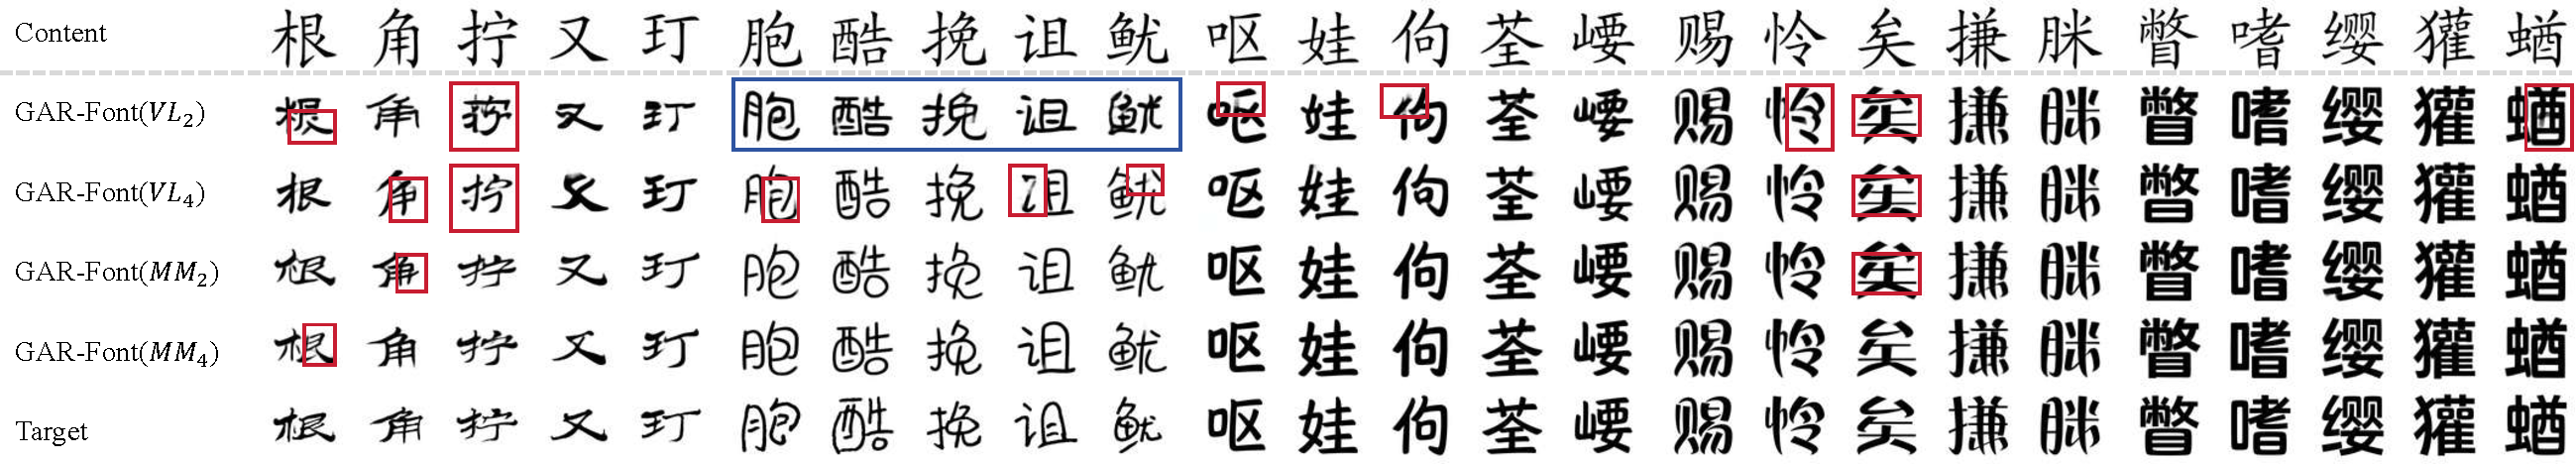
\includegraphics[width=\linewidth]{SUPP_IMGS/EX_Visualization/ABL4_Table_UFUC_Large.pdf}
        \caption{\textit{UFUC}, Large dataset}
        \label{fig: supple_abl4_ufuc_large}
    \end{subfigure}
    \vspace{-3mm}
    \caption{
        Qualitative results on Multimodal Style Encoder's Adaptation under \textit{UFSC} and \textit{UFUC} protocols
        (Large dataset).
        \textcolor{ex1figure_red}{\fbox{\rule{0pt}{4pt}\rule{4pt}{0pt}}} /
        \textcolor{ex1figure_blue}{\fbox{\rule{0pt}{4pt}\rule{4pt}{0pt}}}
        indicate structural errors and style mismatches.
    }
    \label{fig: supple_abl4_all}
    
\end{figure*}
\begin{figure*}[tp]
    \centering

    \begin{subfigure}{0.91\linewidth}
        \centering
        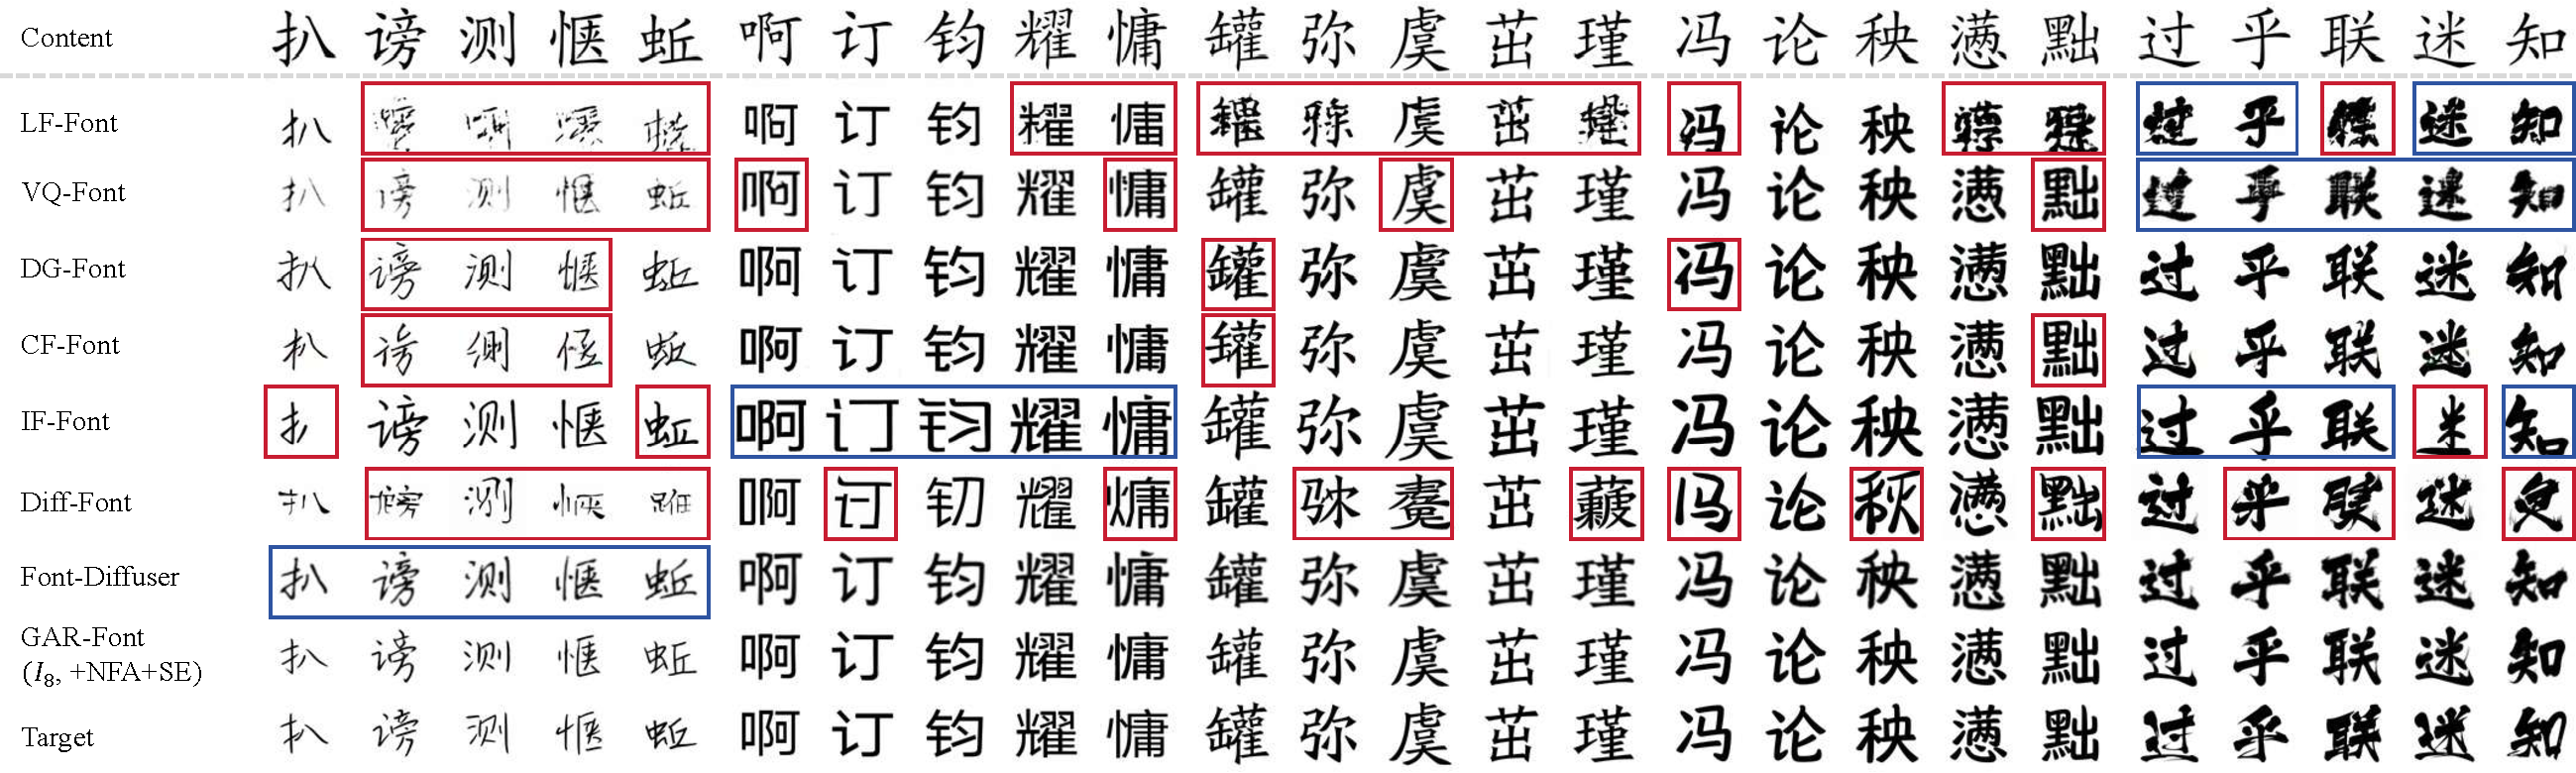
\includegraphics[width=\linewidth]{SUPP_IMGS/EX_Visualization/table_Main1_UFSC_Small.pdf}
        \vspace{-3mm}
        \caption{\textit{UFSC}, Small dataset}
        \label{fig: supple_main1_ufsc_small}
        \vspace{1mm}
    \end{subfigure}

    \begin{subfigure}{0.91\linewidth}
        \centering
        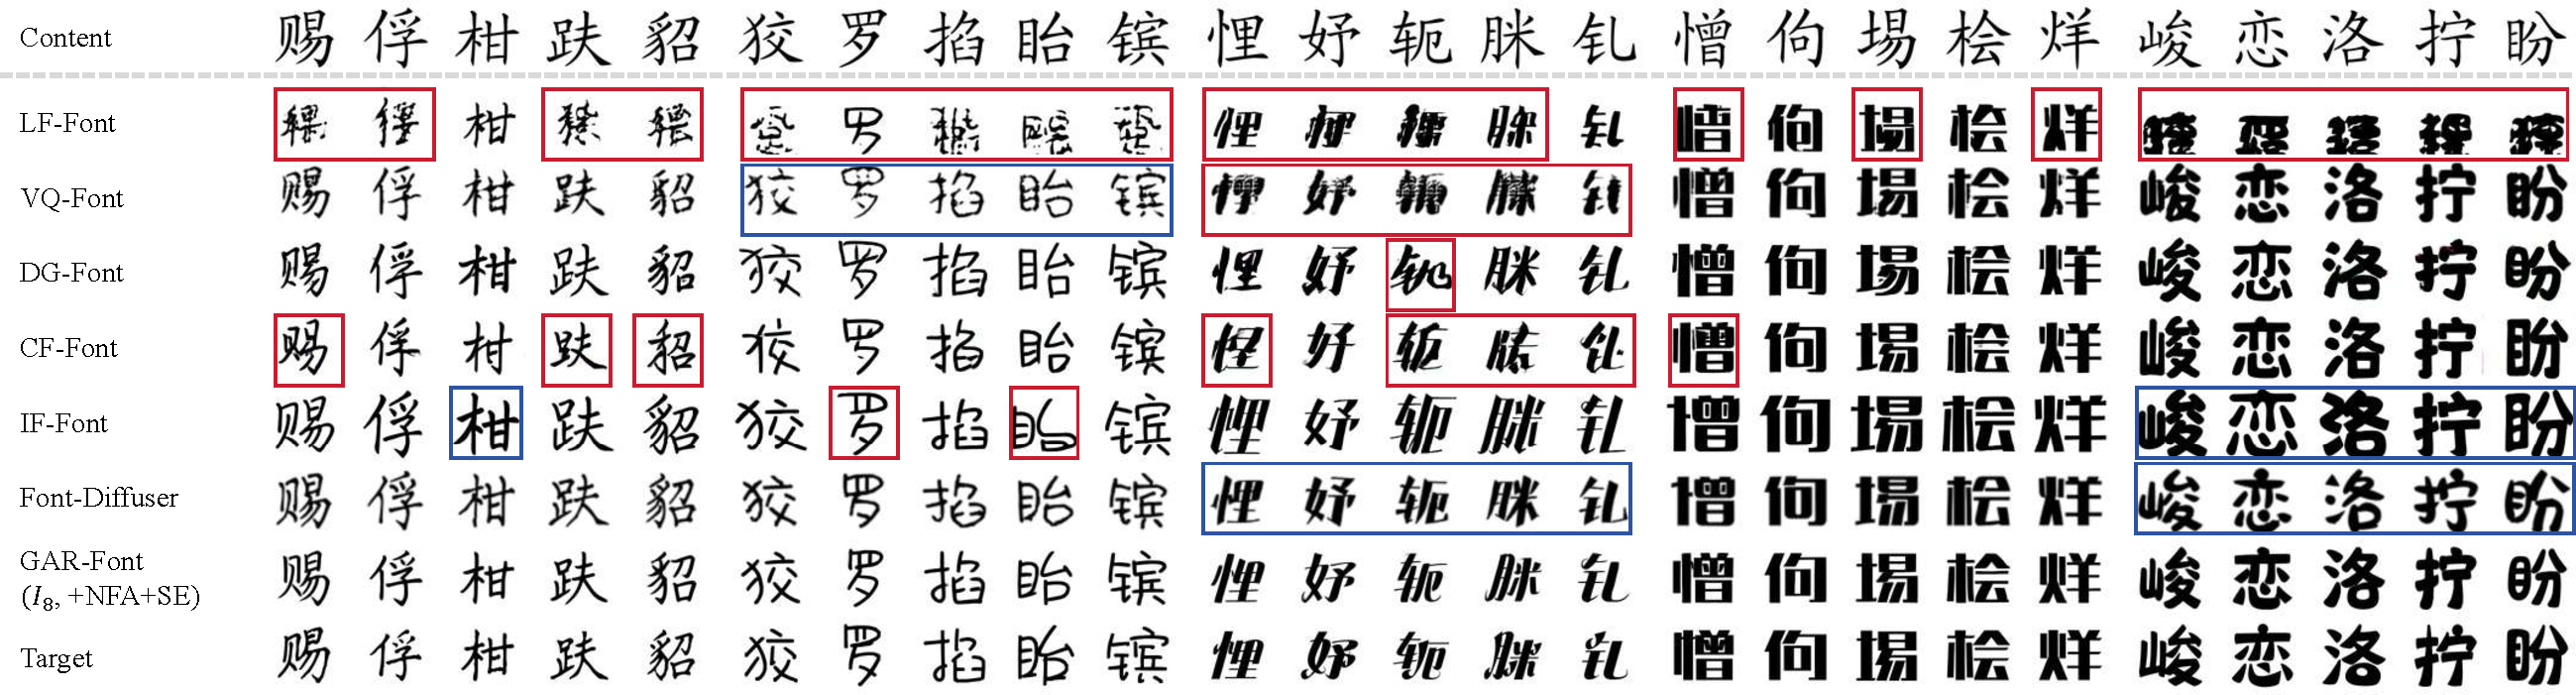
\includegraphics[width=\linewidth]{SUPP_IMGS/EX_Visualization/table_Main1_UFUC_Small.pdf}
        \vspace{-3mm}
        \caption{\textit{UFUC}, Small dataset}
        \vspace{1mm}
        \label{fig: supple_main1_ufuc_small}
    \end{subfigure}

    \begin{subfigure}{0.91\linewidth}
        \centering
        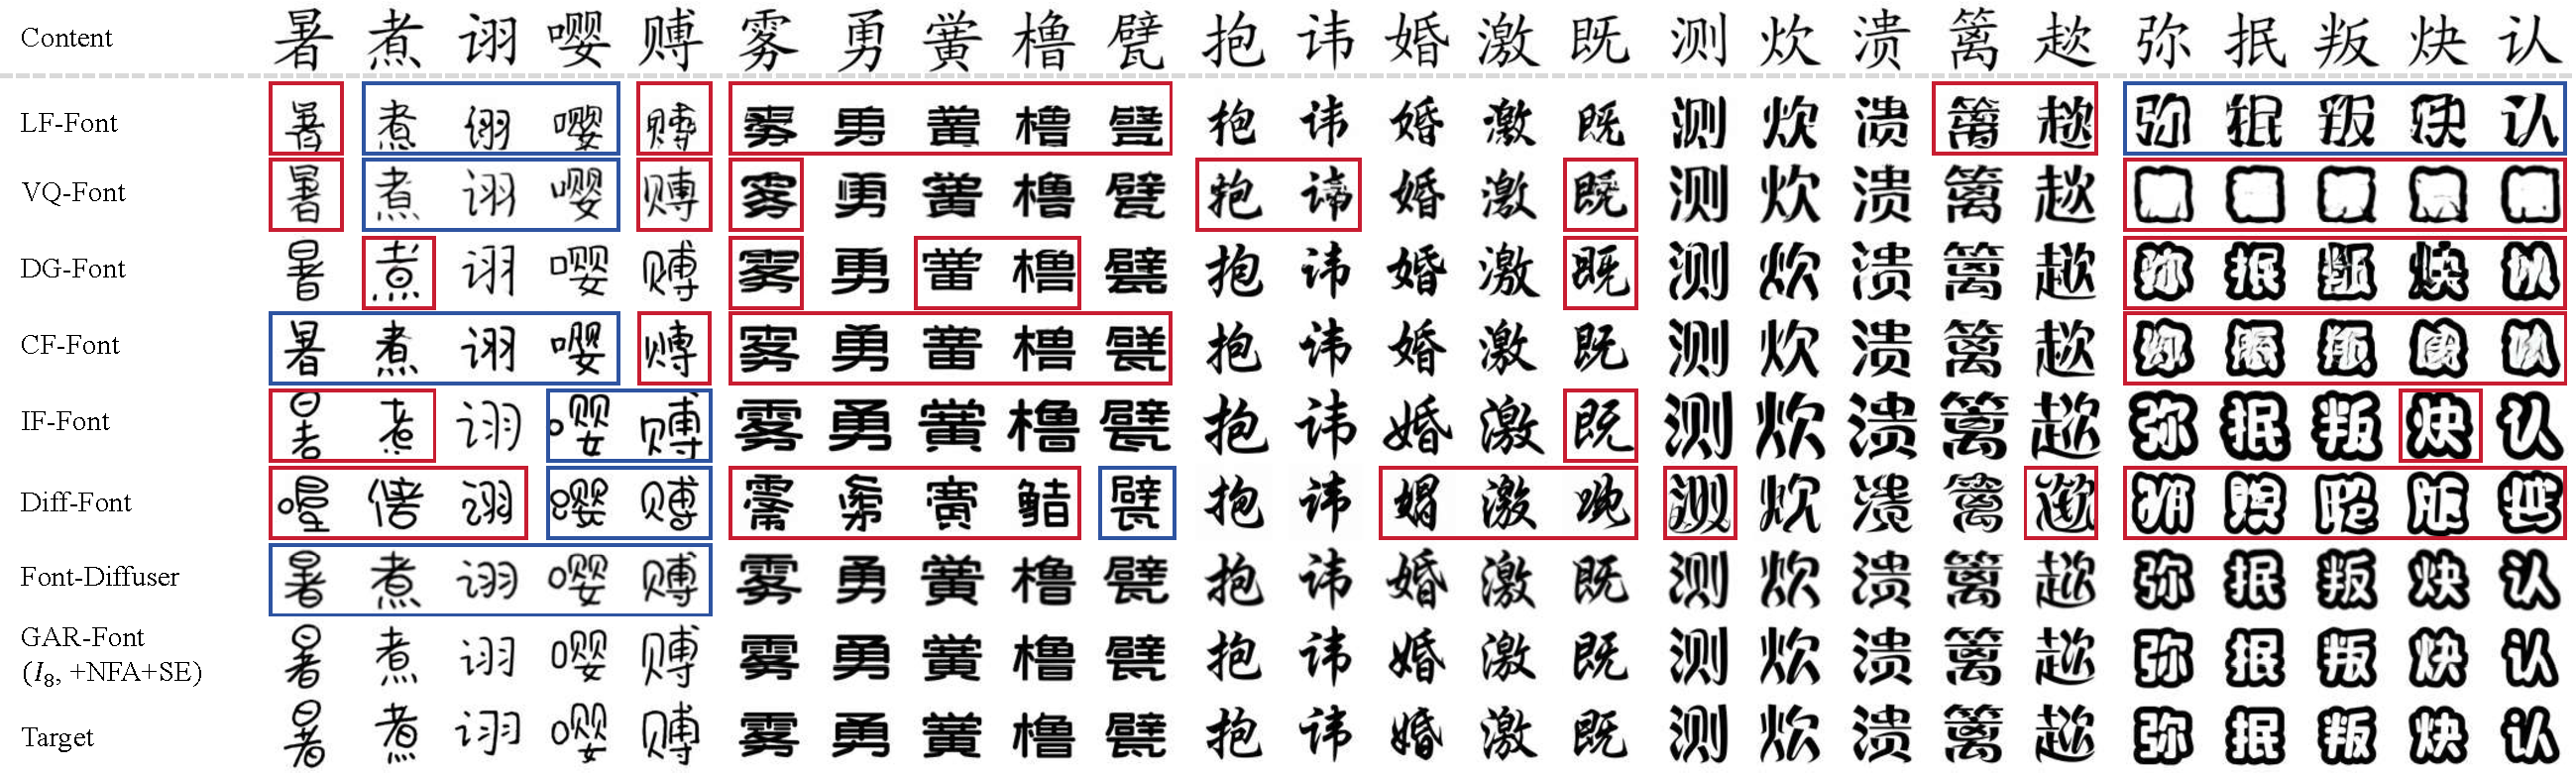
\includegraphics[width=\linewidth]{SUPP_IMGS/EX_Visualization/table_Main1_UFSC_Large.pdf}
        \vspace{-3mm}
        \caption{\textit{UFSC}, Large dataset}
        \vspace{1mm}
        \label{fig: supple_main1_ufsc_large}
    \end{subfigure}

    \begin{subfigure}{0.91\linewidth}
        \centering
        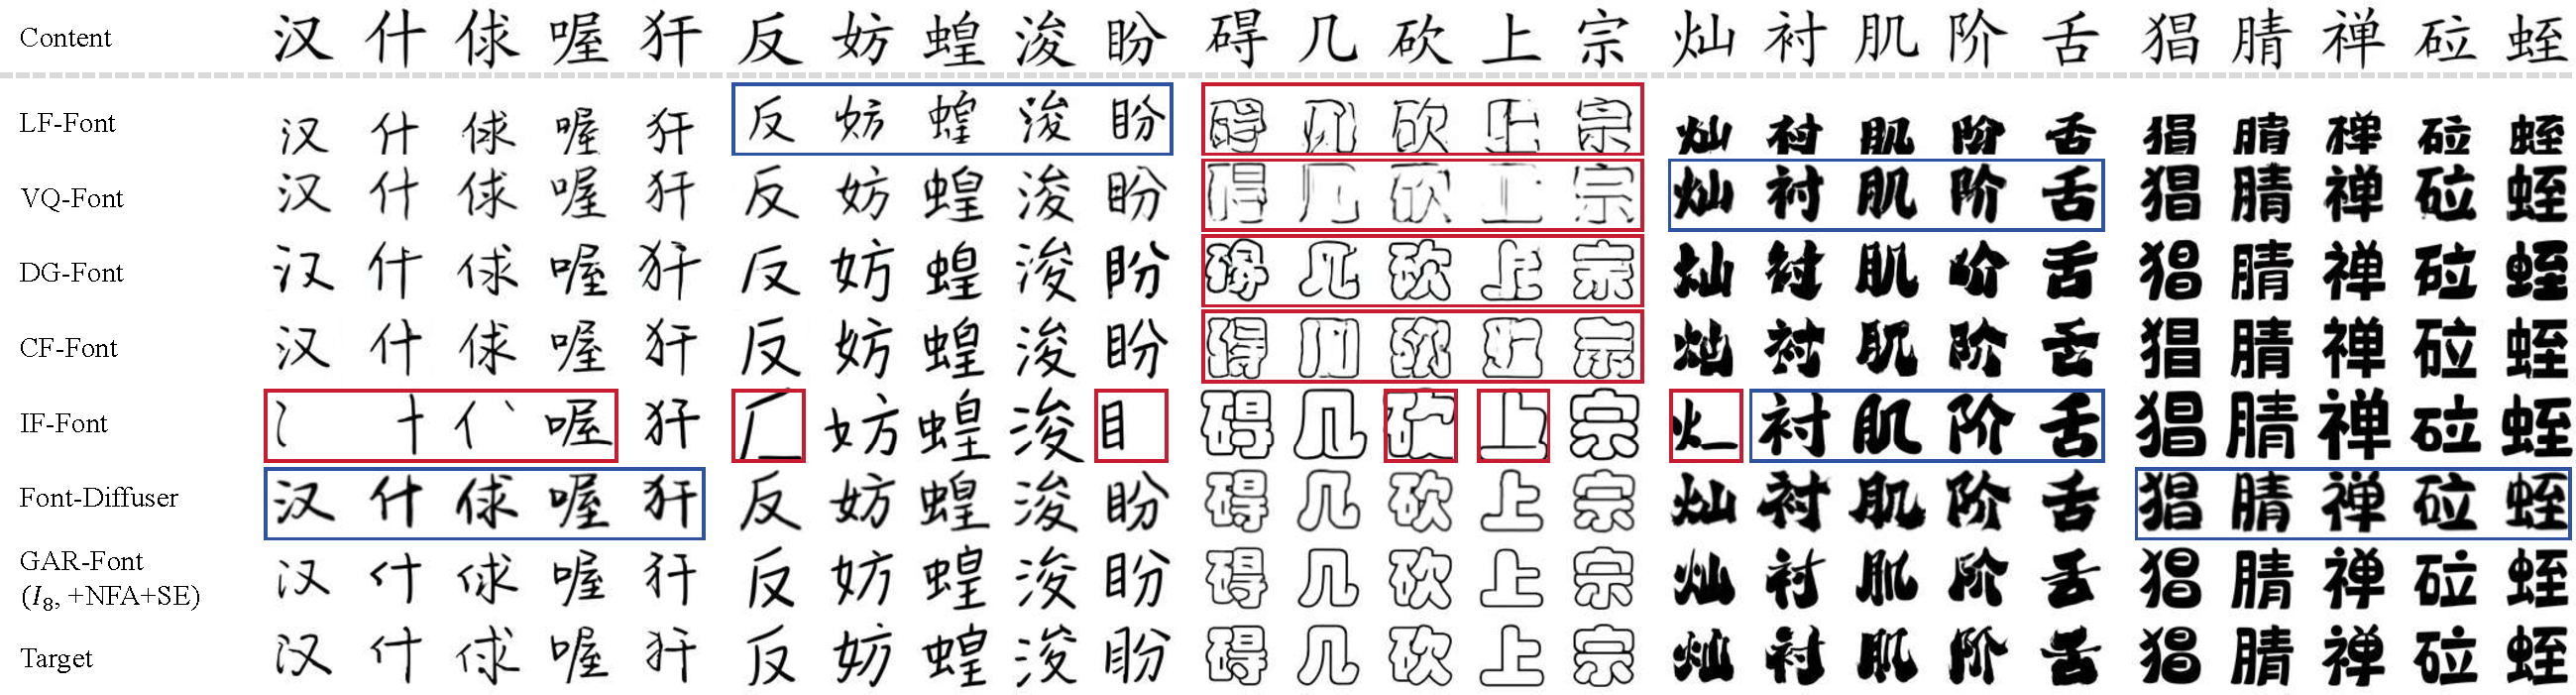
\includegraphics[width=\linewidth]{SUPP_IMGS/EX_Visualization/table_Main1_UFUC_Large.pdf}
        \vspace{-3mm}
        \caption{\textit{UFUC}, Large dataset}
        \vspace{1mm}
        \label{fig: supple_main1_ufuc_large}
    \end{subfigure}
    \vspace{-2mm}
    \caption{
        Qualitative results on vision-only FFG across \textit{UFSC/UFUC} protocols and Small/Large datasets.
        \textcolor{ex1figure_red}{\fbox{\rule{0pt}{4pt}\rule{4pt}{0pt}}} /
        \textcolor{ex1figure_blue}{\fbox{\rule{0pt}{4pt}\rule{4pt}{0pt}}}
        indicate structural errors and style mismatches.
    }
    
    \vspace{-4mm}
    \label{fig: supple_main1_all}
\end{figure*}


\subsection{On Multimodal Style Encoder's Adaptation}
% UFSC,  UFUC,  Large dataset
We compare our decoupled multimodal training paradigm against joint training of the multimodal style encoder. While quantitative results are provided in Section 5.3, we present the full set of qualitative comparisons here.

Figure ~\ref{fig: supple_abl4_all} presents visual comparisons on (\textit{UFSC}, Large) and (\textit{UFUC}, Large). The results reveal that GAR-Font($M_2$/$M_4$), trained with the decoupled training scheme, generate glyphs whose font styles more closely align with the target compared to the jointly trained GAR-Font($VL_2$/$VL_4$). They also demonstrate better character-structure accuracy. The decoupled training strategy enables the model to fully leverage the visual encoder’s representational capacity, thereby preserving fine-grained style features and structural priors that may be harder to retain under joint optimization.


\begin{figure*}[tp] % [p] 强制单独一页
    \centering

    % =========================================
    % 第一组：Pre-Train
    % =========================================
    
    % -------- (a) Pre --------
    \begin{subfigure}{0.92\linewidth} % 建议缩小到 0.9 或 0.85 以防超高
        \centering
        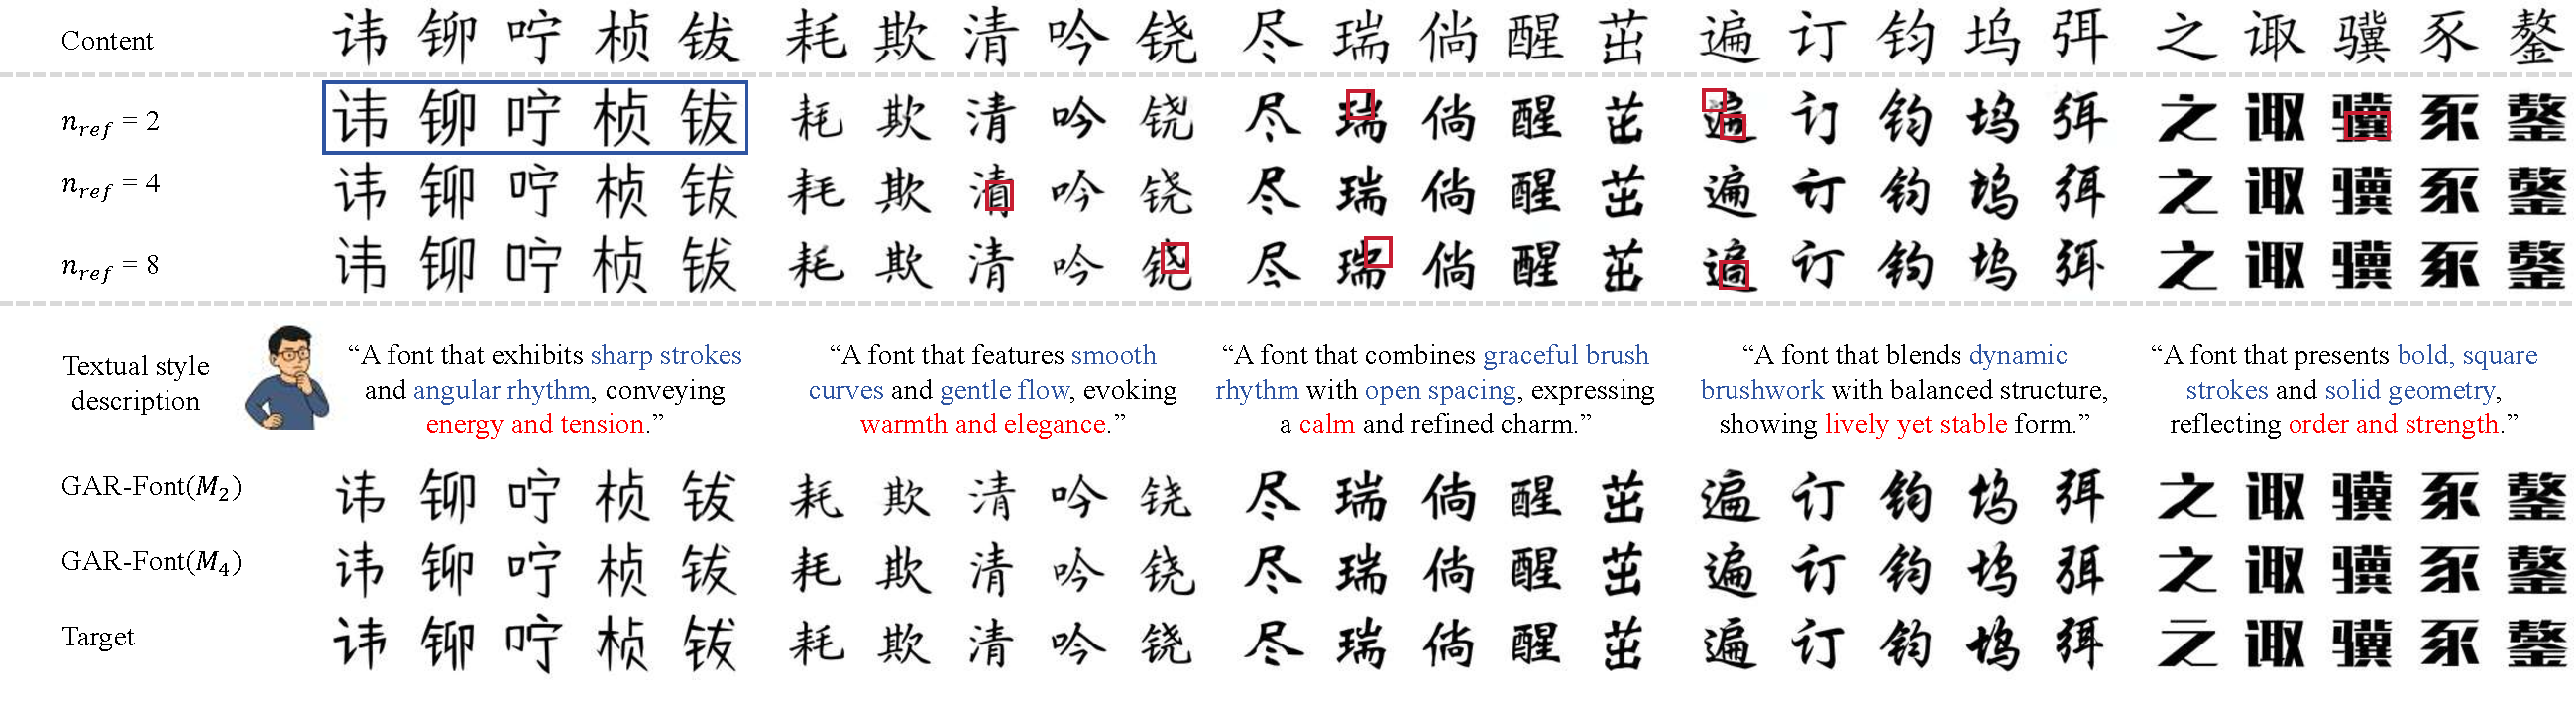
\includegraphics[width=\linewidth]{SUPP_IMGS/EX_Visualization/table2_supple_UFSC_Large_Pre.pdf}
        \caption{\textit{UFSC}, Large dataset}
        \label{fig: supple_main2_ufsc_large_pre}
    \end{subfigure}
    \\ % 强制换行
    \vspace{1mm} % 稍微减少间距
    % -------- (b) Pre --------
    \begin{subfigure}{0.92\linewidth}
        \centering
        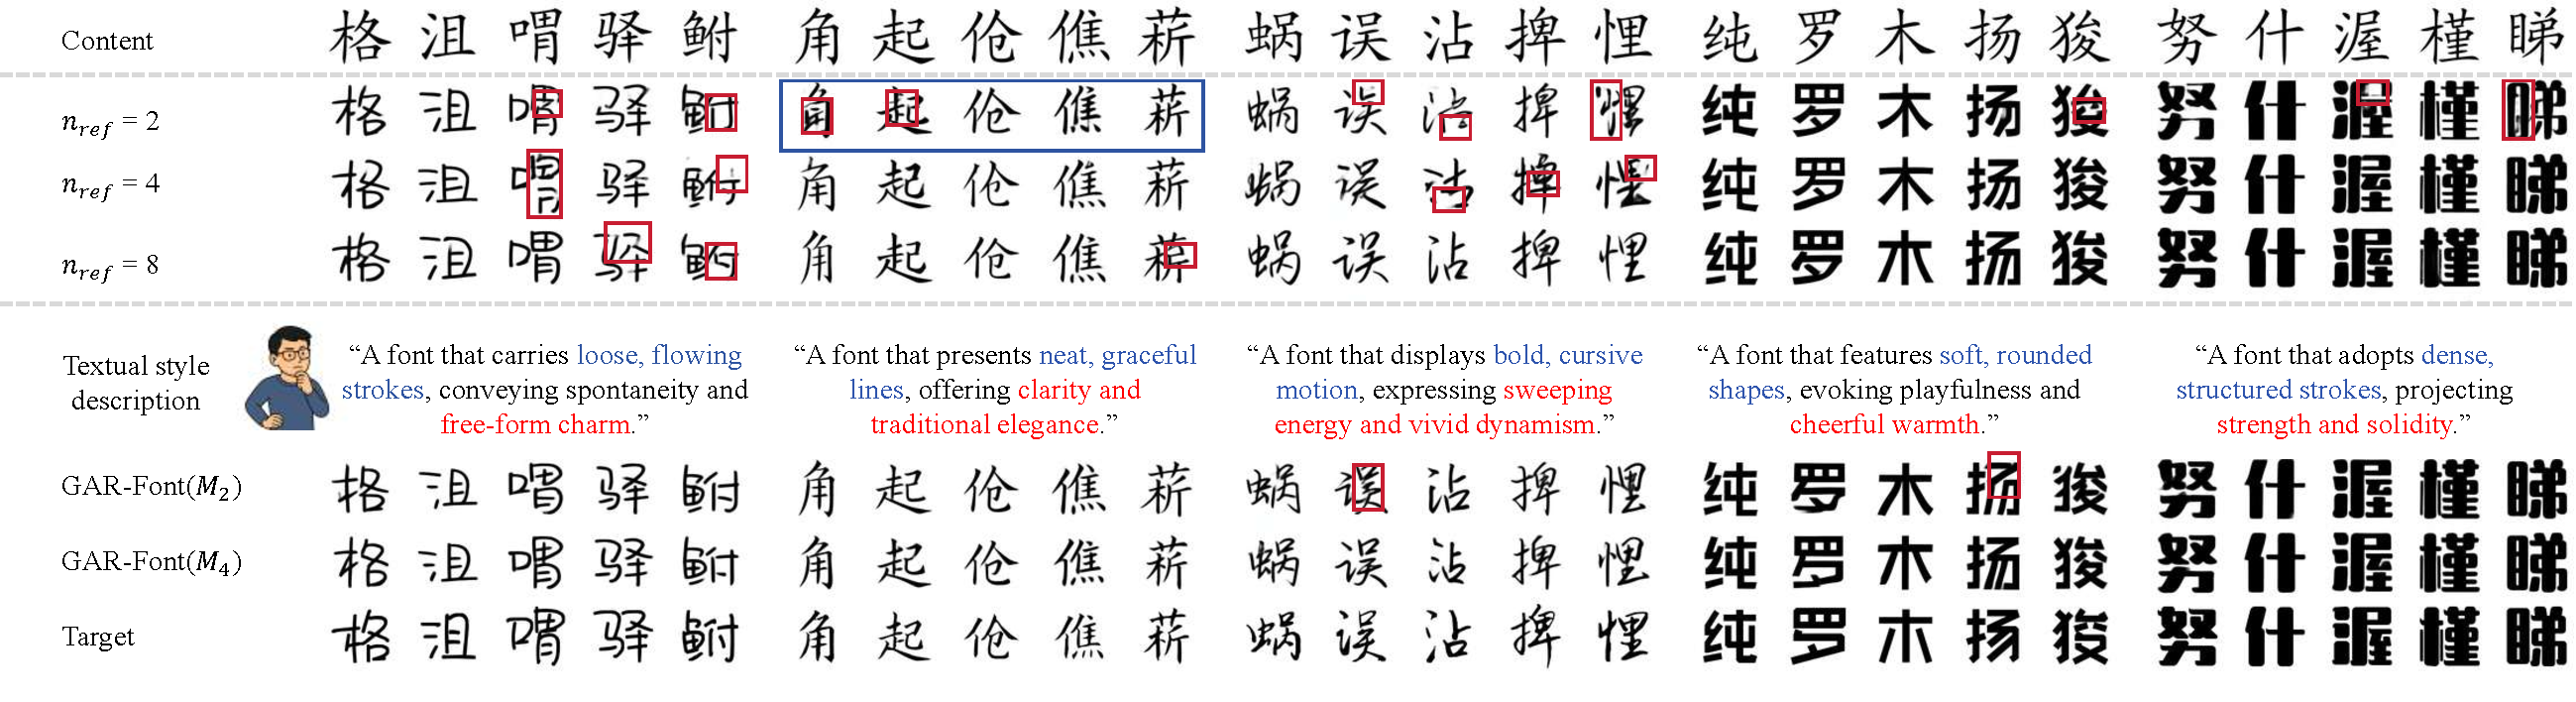
\includegraphics[width=\linewidth]{SUPP_IMGS/EX_Visualization/table2_supple_UFUC_Large_Pre.pdf}
        \caption{\textit{UFUC}, Large dataset}
        \label{fig: supple_main2_ufuc_large_pre}
    \end{subfigure}
    \vspace{-2mm}
    
    % -------- 第一组 Caption --------
    \caption{
        Qualitative results of Pre-Train multimodal FFG under \textit{UFSC} and \textit{UFUC} protocols
        (Large dataset). 
        \textcolor{ex2figure_red}{\fbox{\rule{0pt}{4pt}\rule{4pt}{0pt}}} denotes local slight structural mistakes, 
        and \textcolor{ex2figure_blue}{\fbox{\rule{0pt}{4pt}\rule{4pt}{0pt}}} marks stylistic drift.
    }
    \label{fig: supple_main2_large_pre_all}

    \vspace{1em} % 在两个大图组之间增加明显间距

    % =========================================
    % 第二组：Post-Refine
    % =========================================

    % -------- (a) Post --------
    \begin{subfigure}{0.92\linewidth}
        \centering
        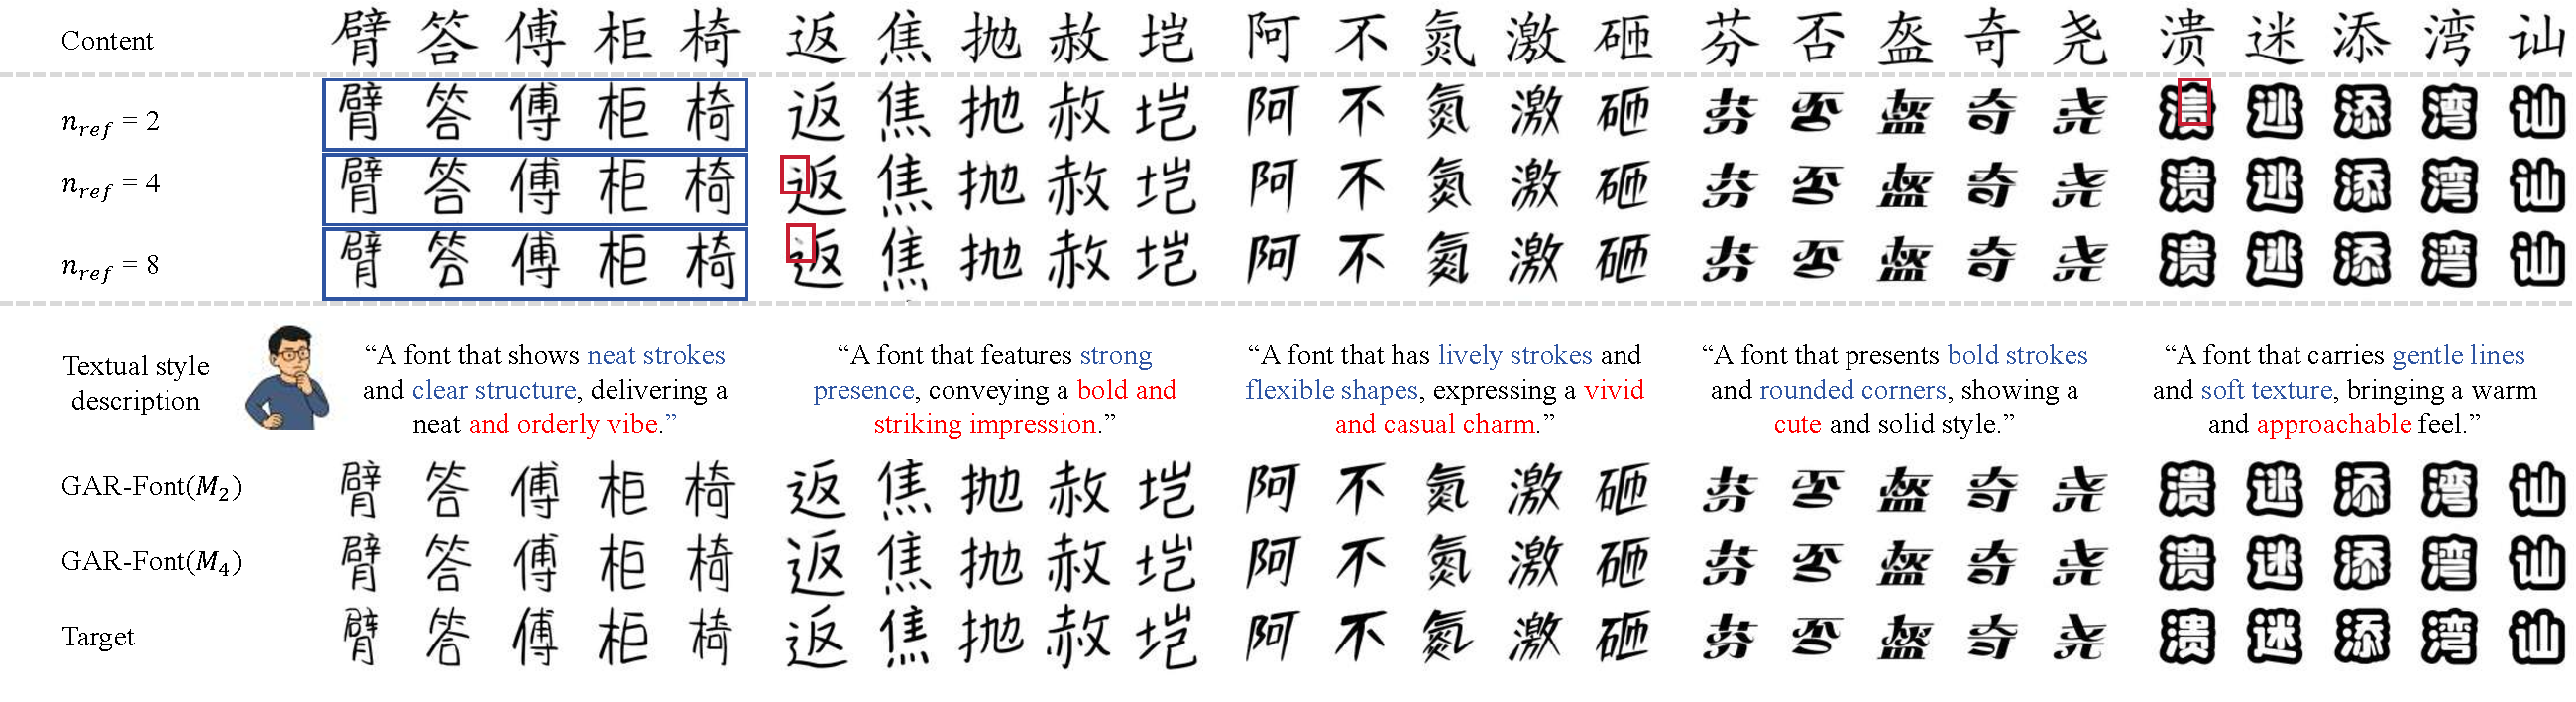
\includegraphics[width=\linewidth]{SUPP_IMGS/EX_Visualization/table2_supple_UFSC_Large_Post.pdf}
        \caption{\textit{UFSC}, Large dataset}
        \label{fig: supple_main2_ufsc_large_post}
    \end{subfigure}
    \\ % 强制换行
    \vspace{1mm}
    % -------- (b) Post --------
    \begin{subfigure}{0.92\linewidth}
        \centering
        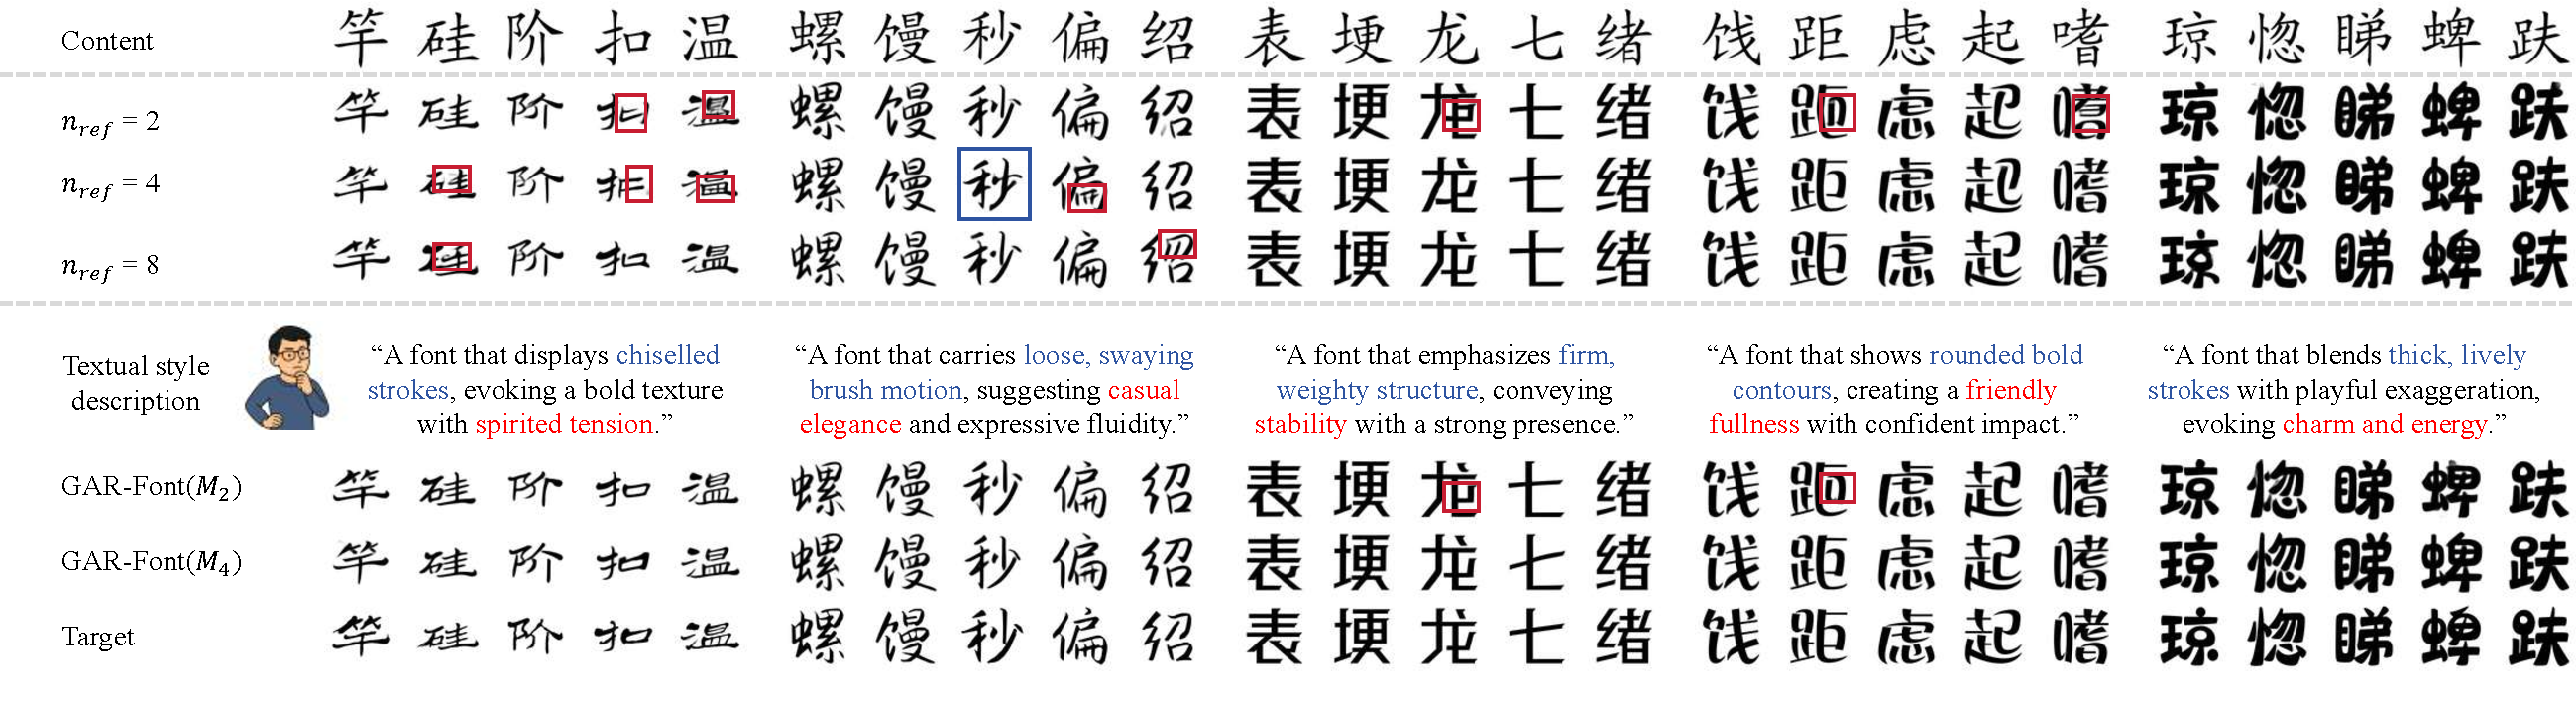
\includegraphics[width=\linewidth]{SUPP_IMGS/EX_Visualization/table2_supple_UFUC_Large_Post.pdf}
        \caption{\textit{UFUC}, Large dataset}
        \label{fig: supple_main2_ufuc_large_post}
    \end{subfigure}
    \vspace{-2mm}

    % -------- 第二组 Caption --------
    \caption{
        Qualitative results of Post-Refine multimodal FFG under \textit{UFSC} and \textit{UFUC} protocols
        (Large dataset). 
        \textcolor{ex2figure_red}{\fbox{\rule{0pt}{4pt}\rule{4pt}{0pt}}} denotes local slight structural mistakes, 
        and \textcolor{ex2figure_blue}{\fbox{\rule{0pt}{4pt}\rule{4pt}{0pt}}} marks stylistic drift.
    }
    \label{fig: supple_main2_large_post}

\end{figure*}




% \begin{figure*}[t]
%     \centering

%     % -------- (a) --------
%     \begin{subfigure}{0.95\linewidth}
%         \centering
%         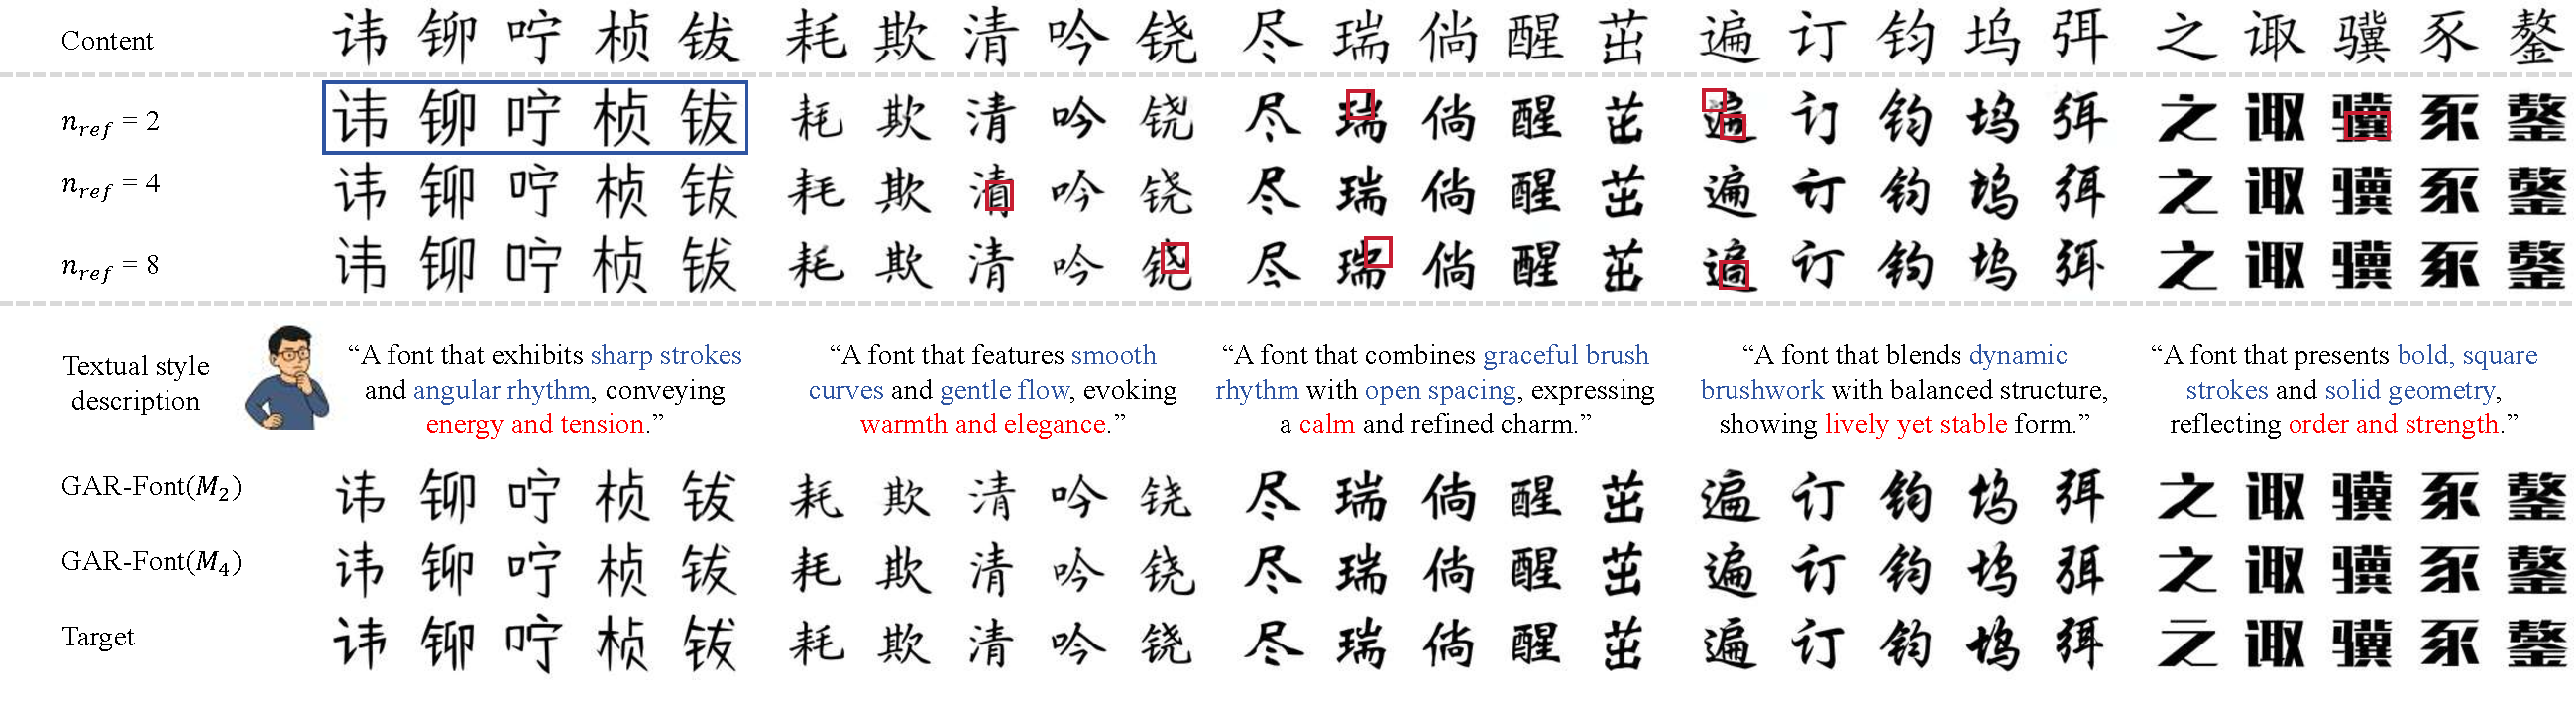
\includegraphics[width=\linewidth]{SUPP_IMGS/EX_Visualization/table2_supple_UFSC_Large_Pre.pdf}
%         \caption{UFSC, \textit{Large} dataset}
%         \label{fig: supple_main2_ufsc_large_pre}
%     \end{subfigure}

%     \vspace{2mm}

%     % -------- (b) --------
%     \begin{subfigure}{0.95\linewidth}
%         \centering
%         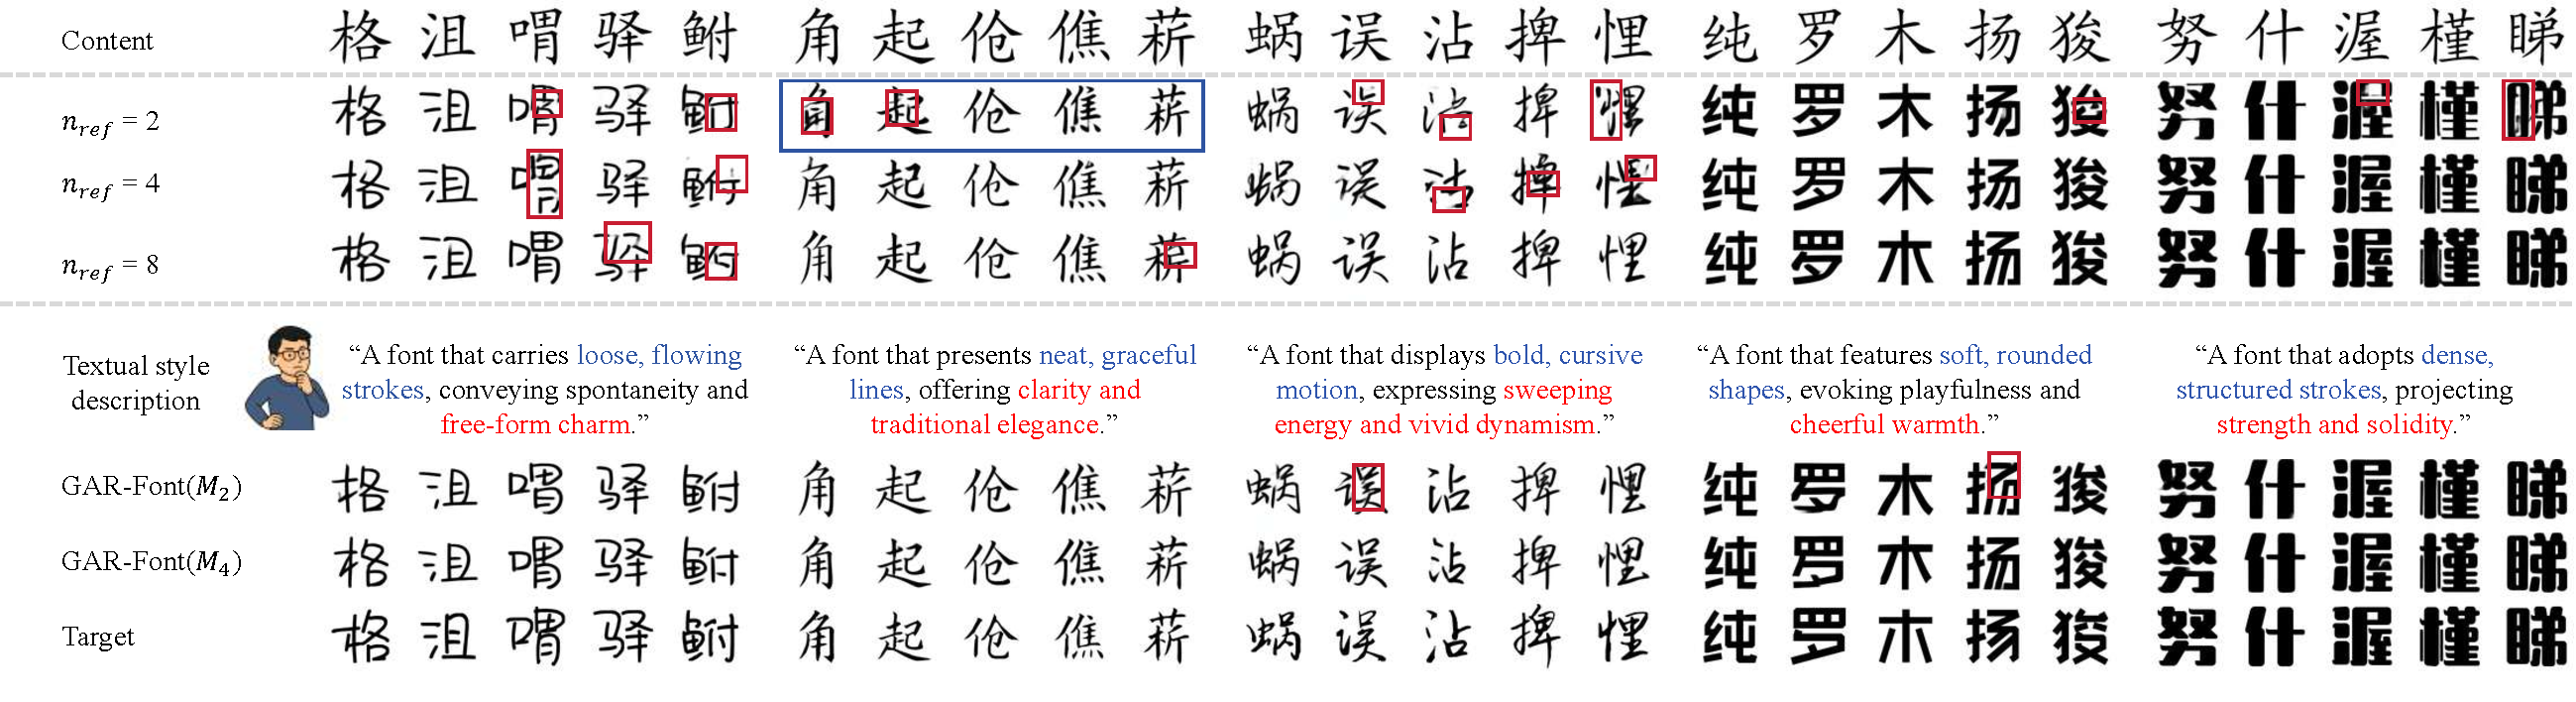
\includegraphics[width=\linewidth]{SUPP_IMGS/EX_Visualization/table2_supple_UFUC_Large_Pre.pdf}
%         \caption{UFUC, \textit{Large} dataset}
%         \label{fig: supple_main2_ufuc_large_pre}
%     \end{subfigure}

%     \vspace{2mm}

%     % -------- main caption --------
%     \caption{
%         Qualitative results on Pre-Train multimodal FFG under UFSC and UFUC protocols
%         (\textit{Large} dataset). 
%         \textcolor{ex2figure_red}{\fbox{\rule{0pt}{4pt}\rule{4pt}{0pt}}} denotes local slight structural mistakes,
%         and \textcolor{ex2figure_blue}{\fbox{\rule{0pt}{4pt}\rule{4pt}{0pt}}} marks samples with stylistic drift.
%     }
%     \label{fig: supple_main2_large_pre_all}
% \end{figure*}



% \begin{figure*}[t]
%     \centering

%     % -------- (a) --------
%     \begin{subfigure}{0.95\linewidth}
%         \centering
%         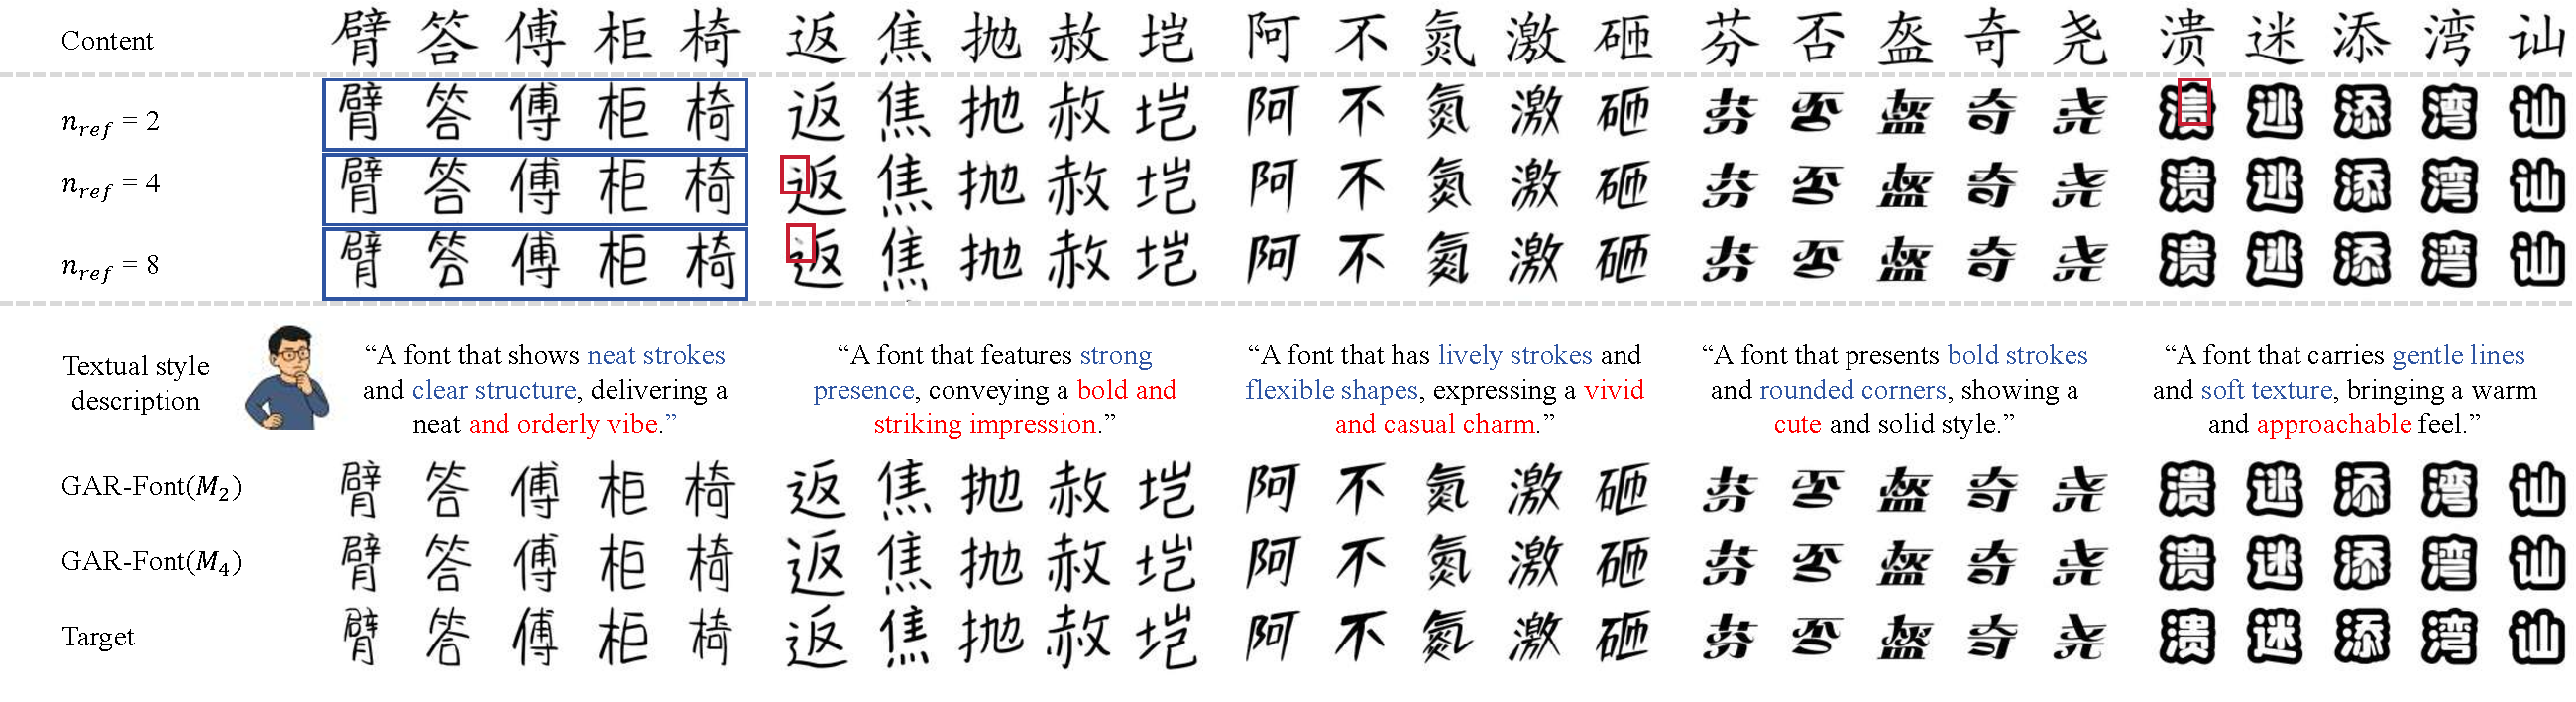
\includegraphics[width=\linewidth]{SUPP_IMGS/EX_Visualization/table2_supple_UFSC_Large_Post.pdf}
%         \caption{UFSC, \textit{Large} dataset}
%         \label{fig: supple_main2_ufsc_large_post}
%     \end{subfigure}

%     \vspace{2mm}

%     % -------- (b) --------
%     \begin{subfigure}{0.95\linewidth}
%         \centering
%         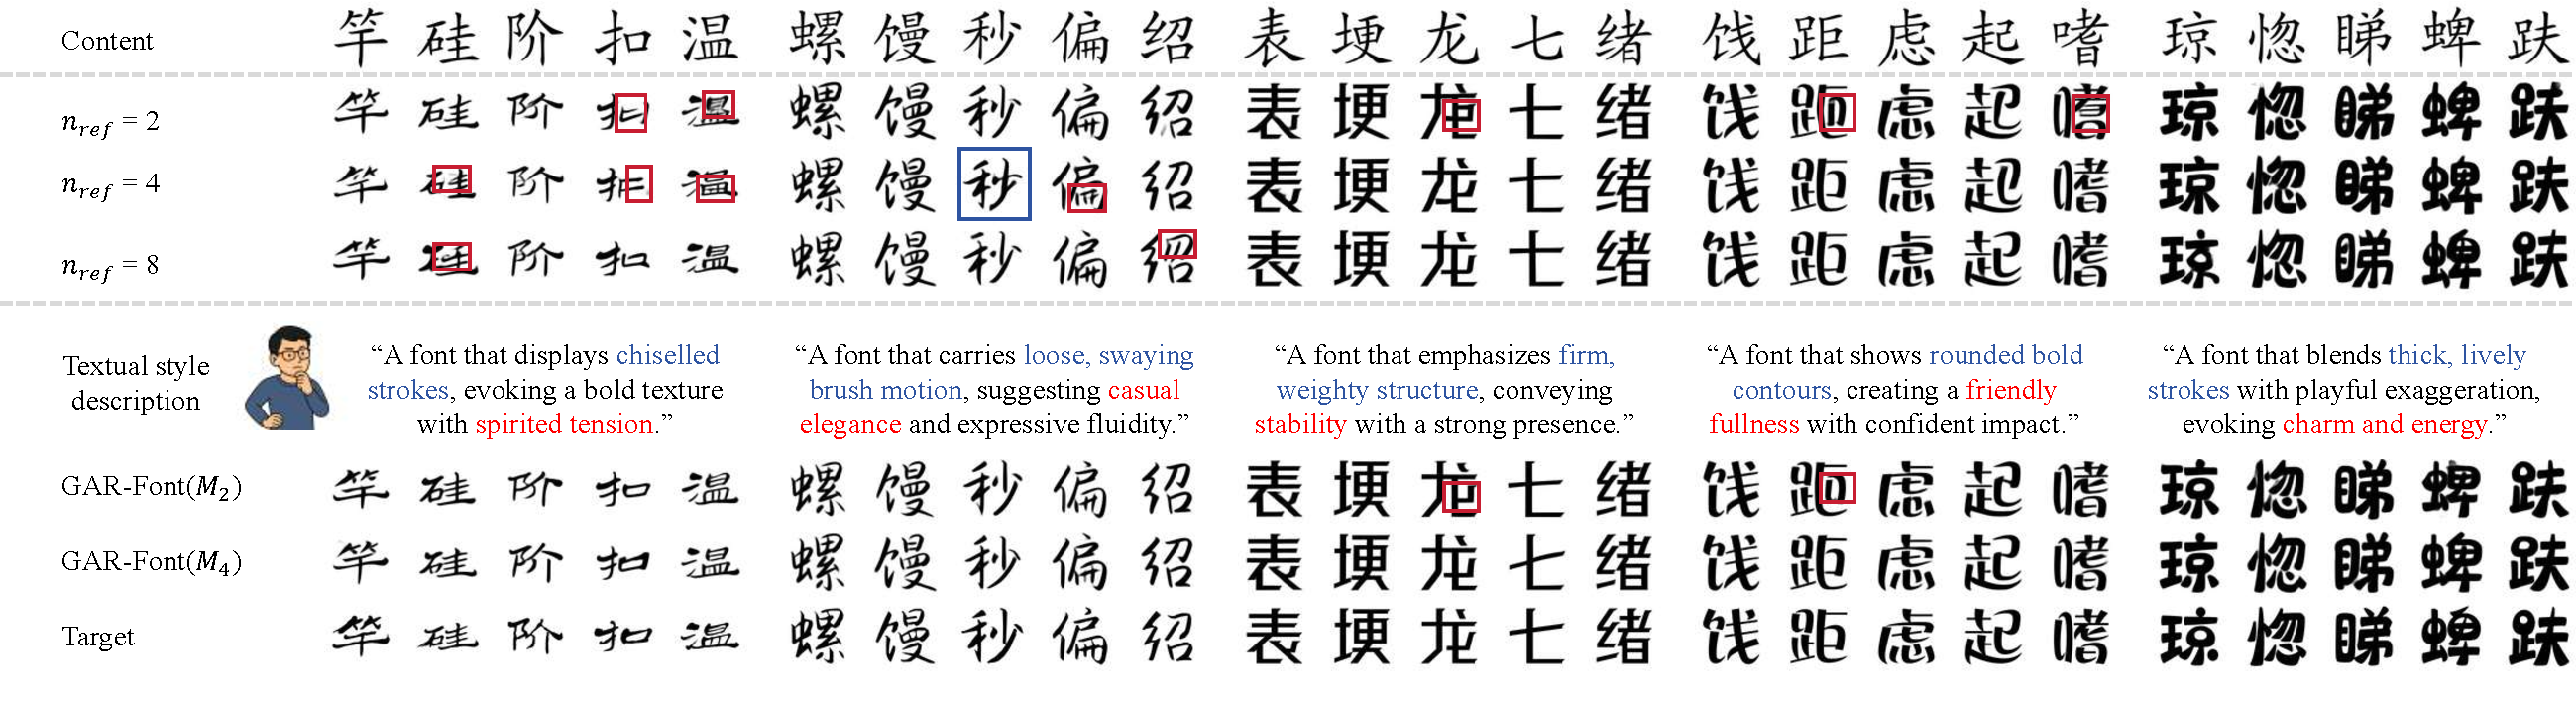
\includegraphics[width=\linewidth]{SUPP_IMGS/EX_Visualization/table2_supple_UFUC_Large_Post.pdf}
%         \caption{UFUC, \textit{Large} dataset}
%         \label{fig: supple_main2_ufuc_large_post}
%     \end{subfigure}

%     \vspace{2mm}

%     % -------- main caption --------
%     \caption{
%         Qualitative results of Post-Refine multimodal FFG under UFSC and UFUC protocols
%         (\textit{Large} dataset). 
%         \textcolor{ex2figure_red}{\fbox{\rule{0pt}{4pt}\rule{4pt}{0pt}}} denotes local slight structural mistakes, 
%         and \textcolor{ex2figure_blue}{\fbox{\rule{0pt}{4pt}\rule{4pt}{0pt}}} marks stylistic drift.
%     }
%     \label{fig: supple_main2_large_post}
% \end{figure*}
\begin{figure*}[t]
  \centering
  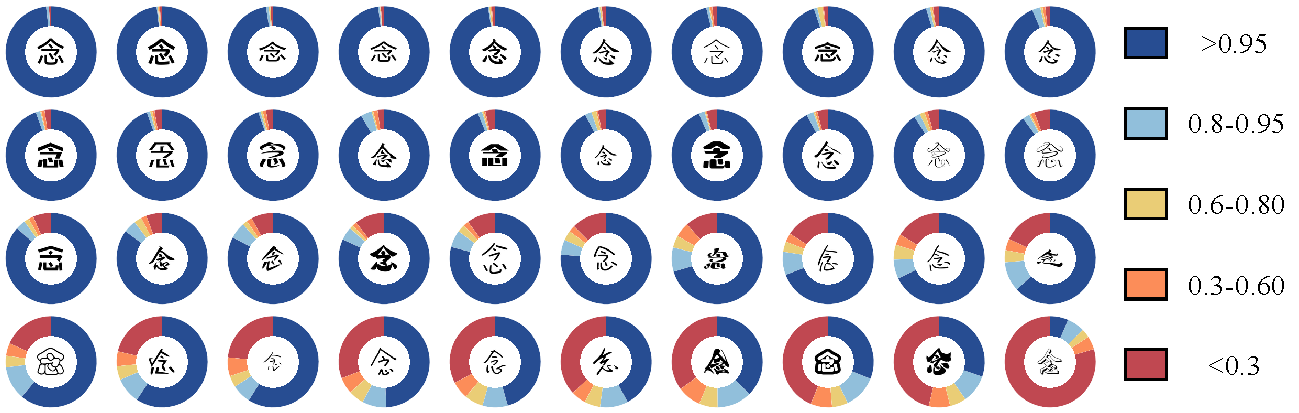
\includegraphics[width=0.95\linewidth]{SUPP_IMGS/Failure_Analysis/analysis_final.pdf}
  \vspace{-3mm}
  \caption{Content confidence distribution of GAR-Font generated characters across different font styles. Each pie chart corresponds to a specific font, indicated by the central character. The color segments represent the proportion of samples falling into different content confidence ranges, highlighting that more complex styles tend to have lower content confidence.}
  \vspace{-3mm}
  \label{fig:supple_analysis}
\end{figure*}



\begin{figure}[t]
  \centering
  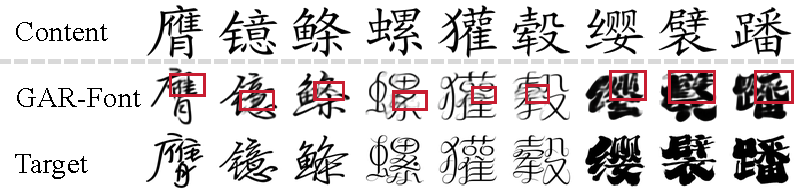
\includegraphics[width=0.95\linewidth]{SUPP_IMGS/Failure_Analysis/Failure_revised.pdf}
  \vspace{-3mm}
  \caption{Failure cases. \textcolor{ex2figure_red}{\fbox{\rule{0pt}{4pt}\rule{4pt}{0pt}}} highlights regions with dense details where GAR-Font tends to produce distorted strokes.}
  \vspace{-3mm}
  \label{fig:supple_failure_cases}
\end{figure}

\section{Visualization Results}
\label{sec:vis_results}
\subsection{Comparison on Few-shot Font Generation}
% UFSC， UFUC，  Large dataset
% UFSC,  UFUC,  Small dataset
We provide complete visualizations for the experiment in Section 5.1. In addition to the main results, Figure~\ref{fig: supple_main1_all} offer a granular analysis of our architectural decisions. 

In Figure~\ref{fig: supple_main1_all}, we show the full qualitative comparisons of visual-only FFG models trained on Small and Large datasets, evaluated under both \textit{UFSC} and \textit{UFUC} protocols. These results indicate that methods such as LF--Font, VQ-Font, DG-Font, CF-Font and Diff-Font often fail to preserve structural fidelity in intricate fonts. IF-Font tends to produce incomplete characters, while Font-Diffuser generates with inaccurate stroke widths. In contrast, GAR-Font($I_8$,+NFA+SE) achieves the best style fidelity while maintaining structural consistency, effectively capturing fine stroke details of the target fonts.


\subsection{Efficient Vision-Language Adaptation}

\subsubsection{Pretrain}
% UFSC， UFUC，  Large dataset

We provide full qualitative results complementing the experiment in Section~5.2. 
In Figure~\ref{fig: supple_main2_large_pre_all}, we show multimodal FFG comparisons under both \textit{UFSC} and \textit{UFUC} settings on the Large dataset, illustrating the improvements introduced by incorporating textual style descriptions in GAR-Font($M_2$) and GAR-Font($M_4$) compared with their vision-only counterparts. With textual style guidance, GAR-Font($M_2$) and GAR-Font($M_4$) better align with the target style, generating glyphs with strokes closely matching the target and improved structural fidelity.


\subsubsection{Post-Refinement}
% UFSC， UFUC，  Large dataset
To further assess the potential of our efficient vision–language adaptation, we apply the complete post-refinement pipeline (NFA and SE) to GAR-Font($M_2$) and GAR-Font($M_4$). 
Figure~\ref{fig: supple_main2_ufsc_large_post} presents qualitative results under \textit{UFSC} and \textit{UFUC} on the Large dataset. Applying NFA and SE post-refinement significantly improves both structural and style fidelity for all models. Textual guidance further enables GAR-Font($M_2$) and GAR-Font($M_4$) to more accurately capture the target style, yielding glyphs with improved style fidelity.

\subsection{More GAR-Font Generation Examples}
To illustrate the capabilities of GAR-Font, we generate the full GB2312 character set for five test fonts with GAR-Font($I_8$, +NFA+SE, trained on Large dataset) and randomly select 1,280 samples from each font. The generated glyphs are shown in Figures ~\ref{fig: add_sheet_1}-~\ref{fig: add_sheet_5} , demonstrating the model’s ability to produce large-scale character sets while faithfully preserving each font’s distinctive stylistic features.


\section{Failure Cases and Analysis}
\label{sec:Failure_cases}

While GAR-Font generally performs well, distortions and blurring occasionally appear in dense-stroke regions of highly complex fonts (\cref{fig:supple_failure_cases}). To investigate this, we applied a content classifier to all \textit{UFUC} samples generated by GAR-Font($I_8$,+NFA+SE), using the softmax output as a measure of content confidence. The results reveal a clear trend: content confidence notably decreases as stylistic complexity increases (\cref{fig:supple_analysis}), suggesting the model sometimes sacrifices structural accuracy to better capture stylistic features.

We hypothesize that this structural degradation results from the error accumulation inherent in autoregressive modeling. Without explicit structural constraints, the model tends to drift when generating intricate stroke patterns. A promising direction for future work is to incorporate explicit structural priors, such as character skeletons or stroke sequences, to guide the generation process. This would help preserve structural fidelity in complex styles.


\begin{figure*}
    \centering
    \includegraphics[width=0.95\linewidth]{SUPP_IMGS/Samples_Sheet/gen_soft_BigruixianBoldkGBV1.0_sample_12.png}
    \vspace{-3mm}
    \caption{Generated glyphs from test fonts using GAR-Font($I_8$, +NFA+SE, Large dataset).}
    \label{fig: add_sheet_1}
    \vspace{-3mm}
\end{figure*}
\clearpage
\begin{figure*}
    \centering
    \includegraphics[width=0.95\linewidth]{SUPP_IMGS/Samples_Sheet/gen_soft_FZBaiZhouRenZheTiS_sample_13.png}
    \vspace{-3mm}
    \caption{Generated glyphs from test fonts using GAR-Font($I_8$, +NFA+SE, Large dataset).}
    \label{fig: add_sheet_2}
    \vspace{-3mm}
\end{figure*}
\clearpage
\begin{figure*}
    \centering
    \includegraphics[width=0.95\linewidth]{SUPP_IMGS/Samples_Sheet/gen_soft_FZSJ-MINGYSJZ_sample_14.png}
    \vspace{-3mm}
    \caption{Generated glyphs from test fonts using GAR-Font($I_8$, +NFA+SE, Large dataset).}
    \label{fig: add_sheet_3}
    \vspace{-3mm}
\end{figure*}
\clearpage
\begin{figure*}
    \centering
    \includegraphics[width=0.95\linewidth]{SUPP_IMGS/Samples_Sheet/gen_soft_MiNiJianYouXian_sample_9.png}
    \vspace{-3mm}
    \caption{Generated glyphs from test fonts using GAR-Font($I_8$, +NFA+SE, Large dataset).}
    \label{fig: add_sheet_4}
    \vspace{-3mm}
\end{figure*}
\clearpage
\begin{figure*}
    \centering
    \includegraphics[width=0.95\linewidth]{SUPP_IMGS/Samples_Sheet/gen_soft_zihun40hao-xiaochengfeifanti-Regular_sample_9.png}
    \vspace{-3mm}
    \caption{Generated glyphs from test fonts using GAR-Font($I_8$, +NFA+SE, Large dataset).}
    \label{fig: add_sheet_5}
    \vspace{-3mm}
\end{figure*}
\clearpage
{
    \small
    \bibliographystyle{ieeenat_fullname}
    \bibliography{main}
}


% \input{sec/2_formatting}
% \input{sec/3_finalcopy}
% WARNING: do not forget to delete the supplementary pages from your submission 
% \clearpage
\setcounter{page}{1}
\setcounter{section}{0}
\setcounter{figure}{0}
\setcounter{table}{0}
\maketitlesupplementary
\renewcommand\thesection{\Alph{section}}
\renewcommand{\thetable}{S\arabic{table}}    % 修改表格标签
\renewcommand{\thefigure}{S\arabic{figure}}  % 修改图片标签

\section{Overview}
\vspace{-1mm}
This supplementary material provides additional details on dataset construction, implementation, and extended experiments supporting the main paper. The sections are organized as follows:
\begin{itemize}
    \item \textbf{\cref{sec:models}}: Model configurations of G-Tok, the autoregressive generator, and the multimodal style encoder.
    \item \textbf{\cref{sec:data_dist}}: Data curation and partitioning, covering both training and evaluation protocols.
    \item \textbf{\cref{sec:quant_ext}}: Extended quantitative results, including scaling analyses of our autoregressive generator.
    \item \textbf{\cref{sec:Ablate}}: Detailed and visualized ablations of key design choices in GAR-Font.
    \item \textbf{\cref{sec:vis_results}}: Extensive qualitative results for visual-only and multimodal FFG, along with error analyses.
    \item \textbf{\cref{sec:Failure_cases}}: Analysis of GAR-Font failure cases in dense-stroke and complex font styles.

    
\end{itemize}

%%%%%%%%%%%%%%%%%%%%%%%%%
\section{Model Configuration}
\label{sec:models}
Table~\ref{tab:model-structure} details the architectural specifications of GAR-Font. The framework relies on three core components: (1) The \textbf{Global-aware Tokenizer (G-Tok)} , which employs a hybrid CNN-ViT architecture to discretize glyphs into a compact codebook ($N=2048$); (2) The \textbf{Autoregressive Generator}, which serves as the synthesis backbone, using a deep Transformer decoder to predict tokens conditioned on aggregated content and style features; and (3) The \textbf{Multimodal Style Encoder}, which utilizes a lightweight adapter to align textual embeddings with visual style representations for text-driven control.
\begin{table}[h]
\centering
\small
\setlength{\tabcolsep}{3pt} % 调小列间距
\begin{tabular}{p{0.8\columnwidth} c}
\toprule
\textbf{Key Components} & \textbf{Params (M)} \\
\midrule
\textbf{G-Tok} & 79.59 \\
CNN Encoder & 28.56 \\
ViT Encoder (layers = 6) & 4.73 \\
Codebook (size = 2048, dim = 8) & 0.02 \\
ViT Decoder (layers = 6) & 4.73 \\
CNN Decoder & 41.42 \\
\midrule
\textbf{AR-Generator} &  346.23 \\
Content Encoder & 28.56 \\
Visual Style Encoder & 2.78 \\
Content-style Aggregator (layers = 3) & 0.79 \\
Transformer Decoder (layers = 24) & 314.10 \\
\midrule
\textbf{Multimodal Style Encoder} & 8.04 \\
Projection & 0.52 \\
Visual Style Encoder & 2.78 \\
Language-Style Adapter (layers = 6) & 4.74 \\
\bottomrule
\end{tabular}
\vspace{-3mm}
\caption{Key GAR-Font components and parameter counts.}
\vspace{-3mm}
\label{tab:model-structure}
\end{table}
\begin{figure}[t]
  \centering
  % You will insert the python-generated PDF here
  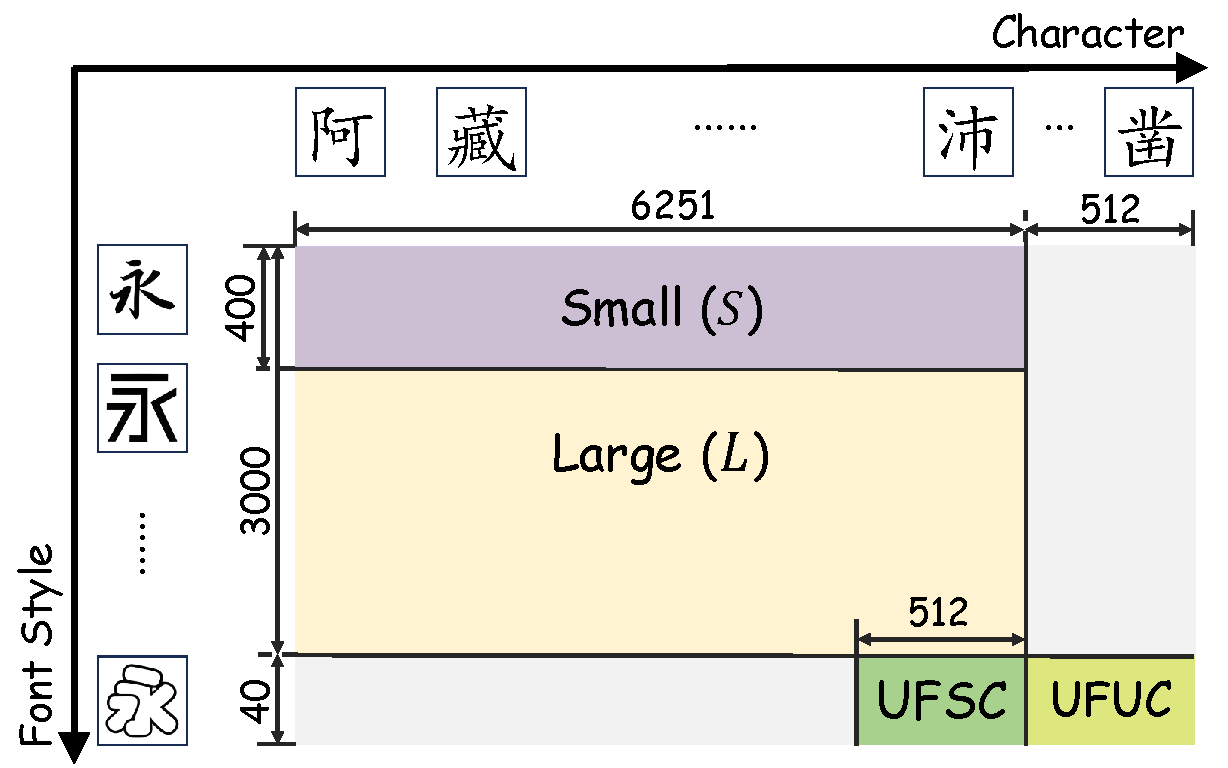
\includegraphics[width=0.95\linewidth]{SUPP_IMGS/data_visualization.pdf} 
  \vspace{-3mm}
  \caption{\textbf{Visual illustration of the dataset partition.} The data is organized along font and character axes. Pre-training utilizes the purple and yellow regions ($S$ and $L$). Evaluation is conducted on the bottom green regions (\textit{UFSC} and \textit{UFUC}), strictly isolating unseen styles and characters.}
  \vspace{-3mm}
  \label{fig:data_viz}
\end{figure}


\section{Data Curation}
\label{sec:data_dist}

\subsection{Data Collection and Statistics}
\label{ssec:data_stats}
We construct a comprehensive font dataset derived from the official GB2312 character set. As illustrated in \cref{fig:data_viz}, the whole training and test dataset is structured as a matrix spanned by two orthogonal axes: \textit{Font Style} (vertical axis) and \textit{Character Category} (horizontal axis). 
The collected data comprises 3,040 fonts and 6,763 characters. 

For training data, along the Character Axis, we split 6,251 training characters (left column) and left 512 characters unseen (right column). The unseen characters are reserved strictly for testing to evaluate the model's capability to generate novel glyph structures. Similarly, the font library is divided into 3,000 training fonts (top rows) and 40 unseen test fonts (bottom rows).


\subsection{Pretraining Data}
\label{ssec:data_pretrain}
The pretraining phase utilizes the data located in the upper-left quadrant of \cref{fig:data_viz}, defined by the intersection of training fonts and training characters. Within this quadrant, we define two configurations to investigate scaling behaviors:
\begin{itemize}[leftmargin=*]
    \item Large ($L$): The full training block consisting of all 3,000 training fonts paired with the 6,251 training characters (represented by the blue region).
    \item Small ($S$): A subset consisting of the first 400 training fonts paired with the same 6,251 characters (represented by the reddish overlay).
\end{itemize}
Training on $S$ versus $L$ allows us to assess the model's data efficiency and performance scaling with respect to the diversity of source styles.

\subsection{Textual Prompt Collection}
\label{ssec:prompt}

To support multimodal few-shot font generation (FFG), we construct a consistent textual prompt set that captures font-level stylistic attributes. For each font, we randomly sample 40 glyph images and jointly input them into Qwen-VL 2.5. The model is instructed to produce a single, unified description summarizing only the visual properties that remain consistent across the full glyph set—such as stroke weight, curvature, structural proportions, spatial rhythm, edge texture, and overall tonal characteristics. This process yields a controlled and stylistically coherent textual representation for each font.

The exact prompt used for textual description extraction is provided below:

\begin{FontExtractPrompt}
You are an experienced typographic style analyst. You are given a set of glyph images belonging to the same font. Your task is to synthesize a unified stylistic description that captures only the consistent, font-level visual attributes shared across the full glyph set.

Your output must adhere to the following specifications:

\textbf{1. Required Format}  

Provide a single paragraph that:

- begins with the phrase “A font that …”,

- contains approximately 45–50 words,

- includes only stylistic properties observable across all glyphs,

- avoids speculative or uncertain expressions.

\textbf{2. Allowed Stylistic Dimensions}  

Constrain your analysis to the following attributes:

- stroke weight (light, medium, bold, uniform, contrasting),

- curvature (straight, angular, rounded, flowing, sharp),

- structural proportions (compact, tall, wide, balanced),

- spacing and rhythm (tight, loose, even, irregular),

- edge rendering (smooth, sharp, rough, brush-like),

- overall tone or mood (elegant, modern, classical, playful, gentle, formal).

\textbf{3. Constraints}  

All statements must be visually grounded in the provided glyph set. Do not reference features specific to individual characters. The description must reflect global stylistic coherence and maintain typographic precision.

\end{FontExtractPrompt}

% \begin{tcolorbox}[
%     colback=gray!5,
%     colframe=gray!35,
%     arc=2mm,
%     boxrule=0.3pt,
%     left=3mm,
%     right=3mm,
%     top=2mm,
%     bottom=2mm
% ]
% \small

% \begin{quote}
% You are assigned the role of a experienced font analyst. A set of glyph images belonging to the same font is provided. Your task is to produce a unified textual description that summarizes the stylistic attributes consistently shared across the glyph set.

% The description must adhere to the following specifications:

% • It must begin with the phrase: “A font that …”.

% • The length must be approximately 45–50 words.

% • The content should focus exclusively on observable and font-level properties, including:

%   – stroke weight (e.g., light, medium, bold, uniform, contrasting)
  
%   – curvature characteristics (e.g., straight, angular, rounded, flowing, sharp)
  
%   – structural proportions (e.g., compact, tall, wide, balanced)
  
%   – spacing and rhythmic organization (e.g., tight, loose, even, irregular)
  
%   – edge rendering (e.g., smooth, sharp, rough, brush-like)
  
%   – overall stylistic tone or mood (e.g., elegant, modern, classical, playful, strong, gentle, formal)

% • The description must avoid speculative or uncertain language (e.g., “seems”, “might”, “appears”).

% • Only stylistic traits observed consistently across the entire glyph set should be included; properties specific to individual characters should be excluded.

% • The output should be a single, self-contained paragraph.

% Generate a concise and precise summary that conforms strictly to these criteria.

% \end{quote}

% \end{tcolorbox}



% You are a professional font style analyst with expertise in abstracting visual attributes from glyph sets. 
% Given a set of glyph images from the same font, produce a concise, high-fidelity textual summary of their shared stylistic characteristics.

% Your output must follow these requirements:
% - Begin the description with: “A font that …”
% - Length must be approximately 45–50 words.
% - Focus strictly on concrete, observable visual attributes, including:
%   • stroke weight (light, medium, bold, uniform, contrasting)
%   • curvature (straight, angular, rounded, flowing, sharp)
%   • proportions (compact, tall, wide, balanced)
%   • spacing & rhythm (tight, loose, even, irregular)
%   • edge texture (smooth, sharp, rough, brush-like)
%   • overall mood (elegant, modern, classical, playful, strong, gentle, formal)
% - The description must be precise, specific, and free of uncertainty (avoid terms such as “seems”, “might”, “probably”, “appears”, “looks like”).
% - Describe only the stylistic properties consistently shared across the entire glyph set, not features of individual characters.



\subsection{Post-Refinement Data}
\label{ssec:data_refine}
To further adapt the model to novel styles and enhance structural consistency, we employ specific data subsets:

\noindent Novel Font Adaptation (NFA). NFA adapts the pre-trained model to the style of the 40 unseen test fonts. For each test font, we sample 128 characters from the 6,251 training character set to serve as style references. This process operates within the vertical column of the training characters but focuses on the unseen font rows.

\noindent Structural Enhancement (SE). SE aims to consolidate global glyph consistency. It utilizes the entire 6,763 characters (spanning both training and unseen characters) but restricts the style to a manageable subset of 400 fonts (sampled from $S$). This ensures the model sees a complete range of structural geometries during the refinement phase without the computational cost of the full font library.


\subsection{Evaluation Data}
\label{ssec:data_eval}
Evaluation is strictly conducted on the held-out bottom rows of the matrix (\cref{fig:data_viz}), ensuring no overlap with the pre-training data. We define two rigorous settings:
\begin{itemize}[leftmargin=*]
    \item \textit{UFSC} (Unseen Fonts, Seen Characters): Represented by the light green region. This setting evaluates the model's ability to stylize known characters into novel font styles.
    \item \textit{UFUC} (Unseen Fonts, Unseen Characters): Represented by the dark green region. This is the most challenging zero-shot setting, where the model must generate glyphs that are novel in both style and structure.
\end{itemize}


%%%%%%%%%%%%%%%%%%%%%%%%%%


\section{More Quantitative Experiments}
\label{sec:quant_ext}
\begin{table}[t]
\centering
\vspace{-3mm}
\caption{Quantitative evaluation on VQ-Font vs. VQ-Font (G). Replacing the original VQ-VAE with G-Tok halves the FID score and boosts content accuracy by nearly 9\%.}
\vspace{-3mm}
\setlength{\tabcolsep}{3pt}
\renewcommand{\arraystretch}{1.1}
\small
\resizebox{\linewidth}{!}{
\begin{tabular}{lcccccc}
\toprule
\multicolumn{7}{c}{\textbf{Unseen Fonts Seen Characters (UFSC)}} \\
\midrule
Method & RMSE$\downarrow$ & SSIM$\uparrow$ & LPIPS$\downarrow$ & FID$\downarrow$ & Acc(C)$\uparrow$ & Acc(S)$\uparrow$ \\
\midrule
VQ\_Font        & 0.2727 & 0.5642 & 0.1830 & 35.2472 & 0.8763 & 0.0016 \\
VQ\_Font (G)    & \textbf{0.2725} & \textbf{0.5644} & \textbf{0.1731} & \textbf{17.3296} & \textbf{0.9646} & \textbf{0.0022} \\
\midrule\midrule
\multicolumn{7}{c}{\textbf{Unseen Fonts Unseen Characters (UFUC)}} \\
\midrule
Method & RMSE$\downarrow$ & SSIM$\uparrow$ & LPIPS$\downarrow$ & FID$\downarrow$ & Acc(C)$\uparrow$ & Acc(S)$\uparrow$ \\
\midrule
VQ\_Font        & 0.2744 & 0.5616 & 0.1822 & 36.7914 & 0.8882 & 0.0016 \\
VQ\_Font (G)    & \textbf{0.2732} & \textbf{0.5637} & \textbf{0.1731} & \textbf{17.9152} & \textbf{0.9653} &\textbf{0.0023} \\
\bottomrule
\end{tabular}
}
\label{tab:quant_eval_gtok_adaptation}
\end{table}
\begin{figure}[t]
  \centering
  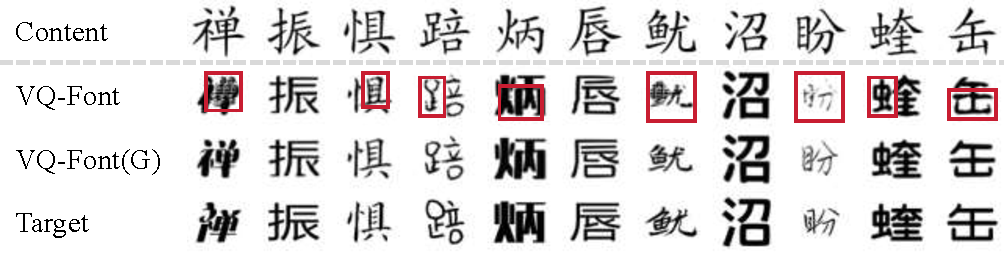
\includegraphics[width=0.95\linewidth]{SUPP_IMGS/EX_Visualization/VQ_G.pdf} 
  \caption{
Qualitative comparison on VQ-Font vs. VQ-Font (G). 
\textcolor{ex2figure_red}{\fbox{\rule{0pt}{4pt}\rule{4pt}{0pt}}} marks structural errors in the generated glyph. 
G-Tok improves structure preservation and produces more faithful font styles.
}
  \label{fig:supple_vq_g_ufuc}
\end{figure}


\begin{table*}[!t]
\centering
\caption{Quantitative evaluation of Multimodal FFG with full post-refinement (NFA and SE) on Unseen Fonts. All models listed are post-trained with NFA and SE stages on the Large dataset.}
\vspace{-2mm}
\setlength{\tabcolsep}{3pt}
\renewcommand{\arraystretch}{1.05}
\resizebox{0.95\textwidth}{!}{
\begin{tabular}{l | c c c c c c | c c c c c c }
\toprule
Method & \multicolumn{6}{c|}{Unseen Fonts Seen Characters (UFSC)} & \multicolumn{6}{c}{Unseen Fonts Unseen Characters (UFUC)} \\
\cmidrule(lr){2-7} \cmidrule(lr){8-13}
 & RMSE$\downarrow$ & SSIM$\uparrow$ & LPIPS$\downarrow$ & FID$\downarrow$ & Acc(C)$\uparrow$ & Acc(S)$\uparrow$
 & RMSE$\downarrow$ & SSIM$\uparrow$ & LPIPS$\downarrow$ & FID$\downarrow$ & Acc(C)$\uparrow$ & Acc(S)$\uparrow$ \\
\hline
$n_\text{ref}=2$ & 0.2501 & 0.6438 & 0.0888 & 10.1464 & \textbf{0.9851} & 0.3314 & 0.2701 & 0.5987 & 0.1069 & 9.4294 & 0.8720 & 0.3433 \\
$n_\text{ref}=4$ & 0.2437 & 0.6552 & 0.0848 & 9.5960  & 0.9839 & 0.3711 & 0.2692 & 0.6007 & 0.1049 & 9.0877 & 0.8828 & 0.3835 \\
$n_\text{ref}=8$ & 0.2398 & 0.6627 & 0.0831 & \textbf{8.3751}  & 0.9776 & 0.4154 & \textbf{0.2508} & \textbf{0.6377} & \textbf{0.0908} & \textbf{7.2034} & \textbf{0.9068} & 0.4183 \\
\Xhline{1.2pt}
GAR-Font($M_2$) & 0.2361 & 0.6707 & 0.0799 & 8.8867  & 0.9817 & 0.4508 & 0.2527 & 0.6352 & 0.0909 & 8.1444 & 0.9029 & 0.4247 \\
GAR-Font($M_4$) & \textbf{0.2358} & \textbf{0.6712} & \textbf{0.0796} & 8.8073  & 0.9800 & \textbf{0.4566} & 0.2524 & 0.6353 & \textbf{0.0908} & 8.0699 & 0.9023 & \textbf{0.4391} \\
\bottomrule
\end{tabular}
}
\label{tab:quant_eval_ref_mm}
\end{table*}
\begin{figure*}[!t]
    \centering
    \begin{minipage}{0.495\linewidth}
        \centering
        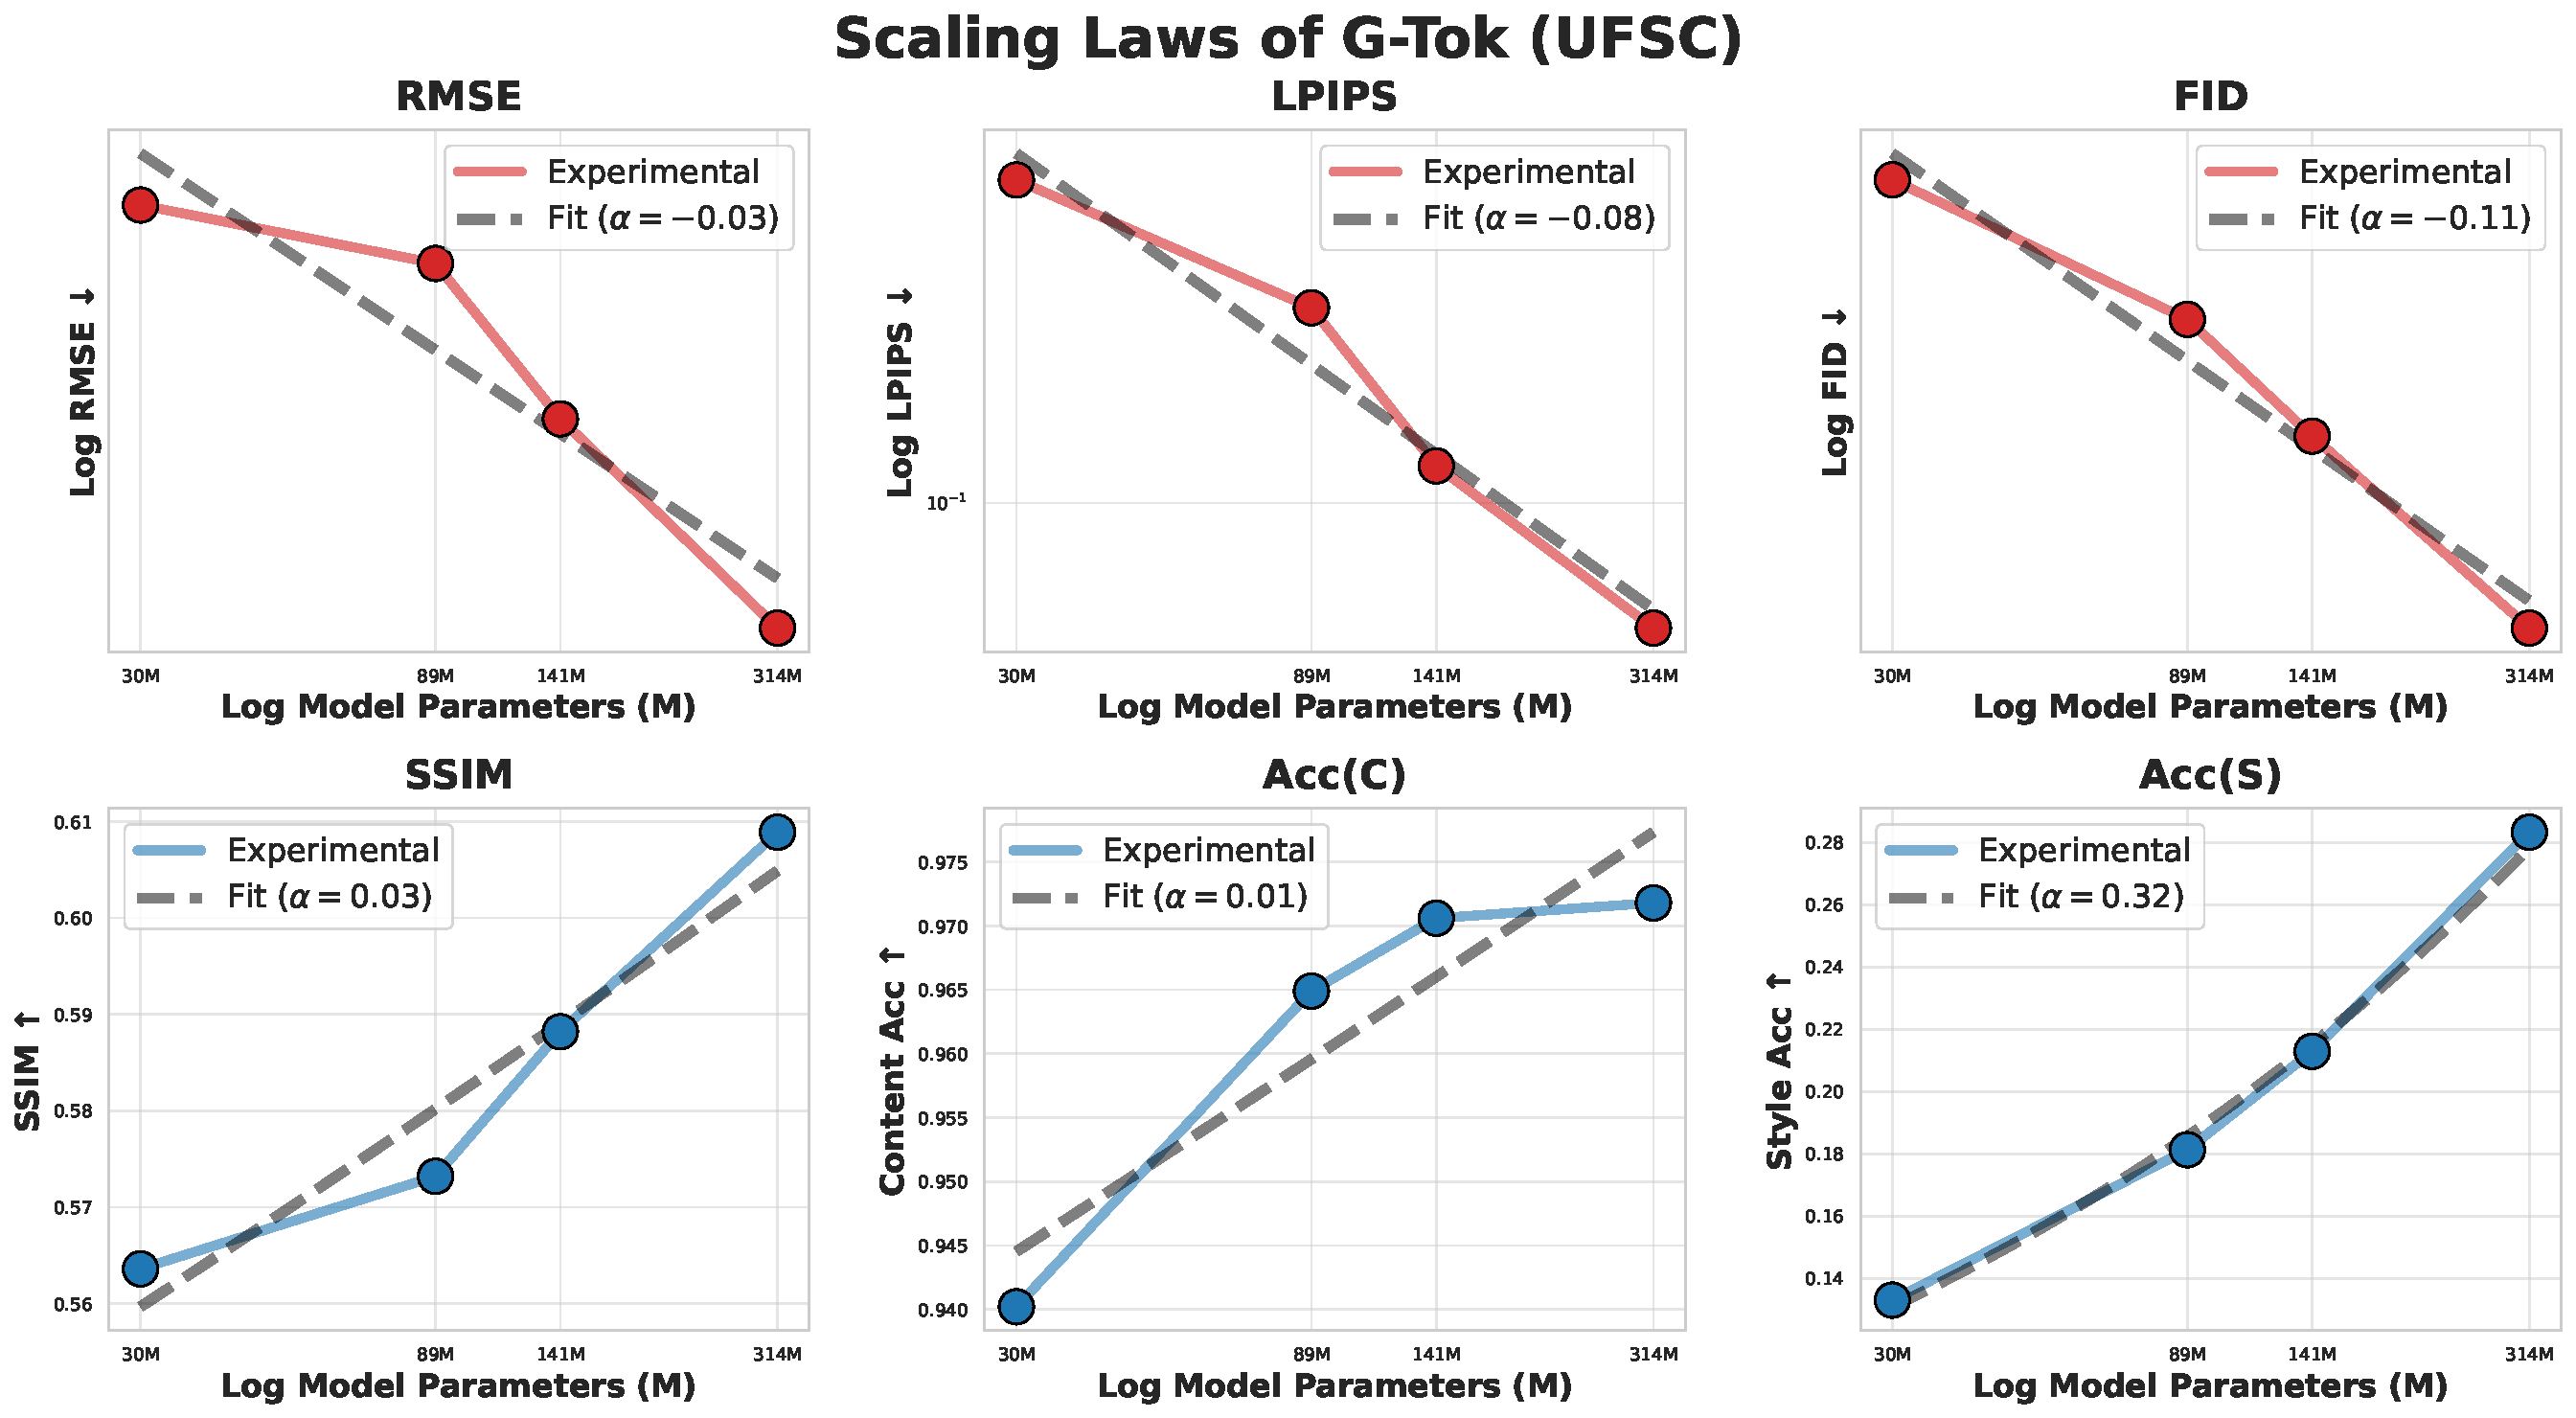
\includegraphics[width=\linewidth]{SUPP_IMGS/scaling_law_UFSC.pdf}
    \end{minipage}
    \hfill
    \begin{minipage}{0.495\linewidth}
        \centering
        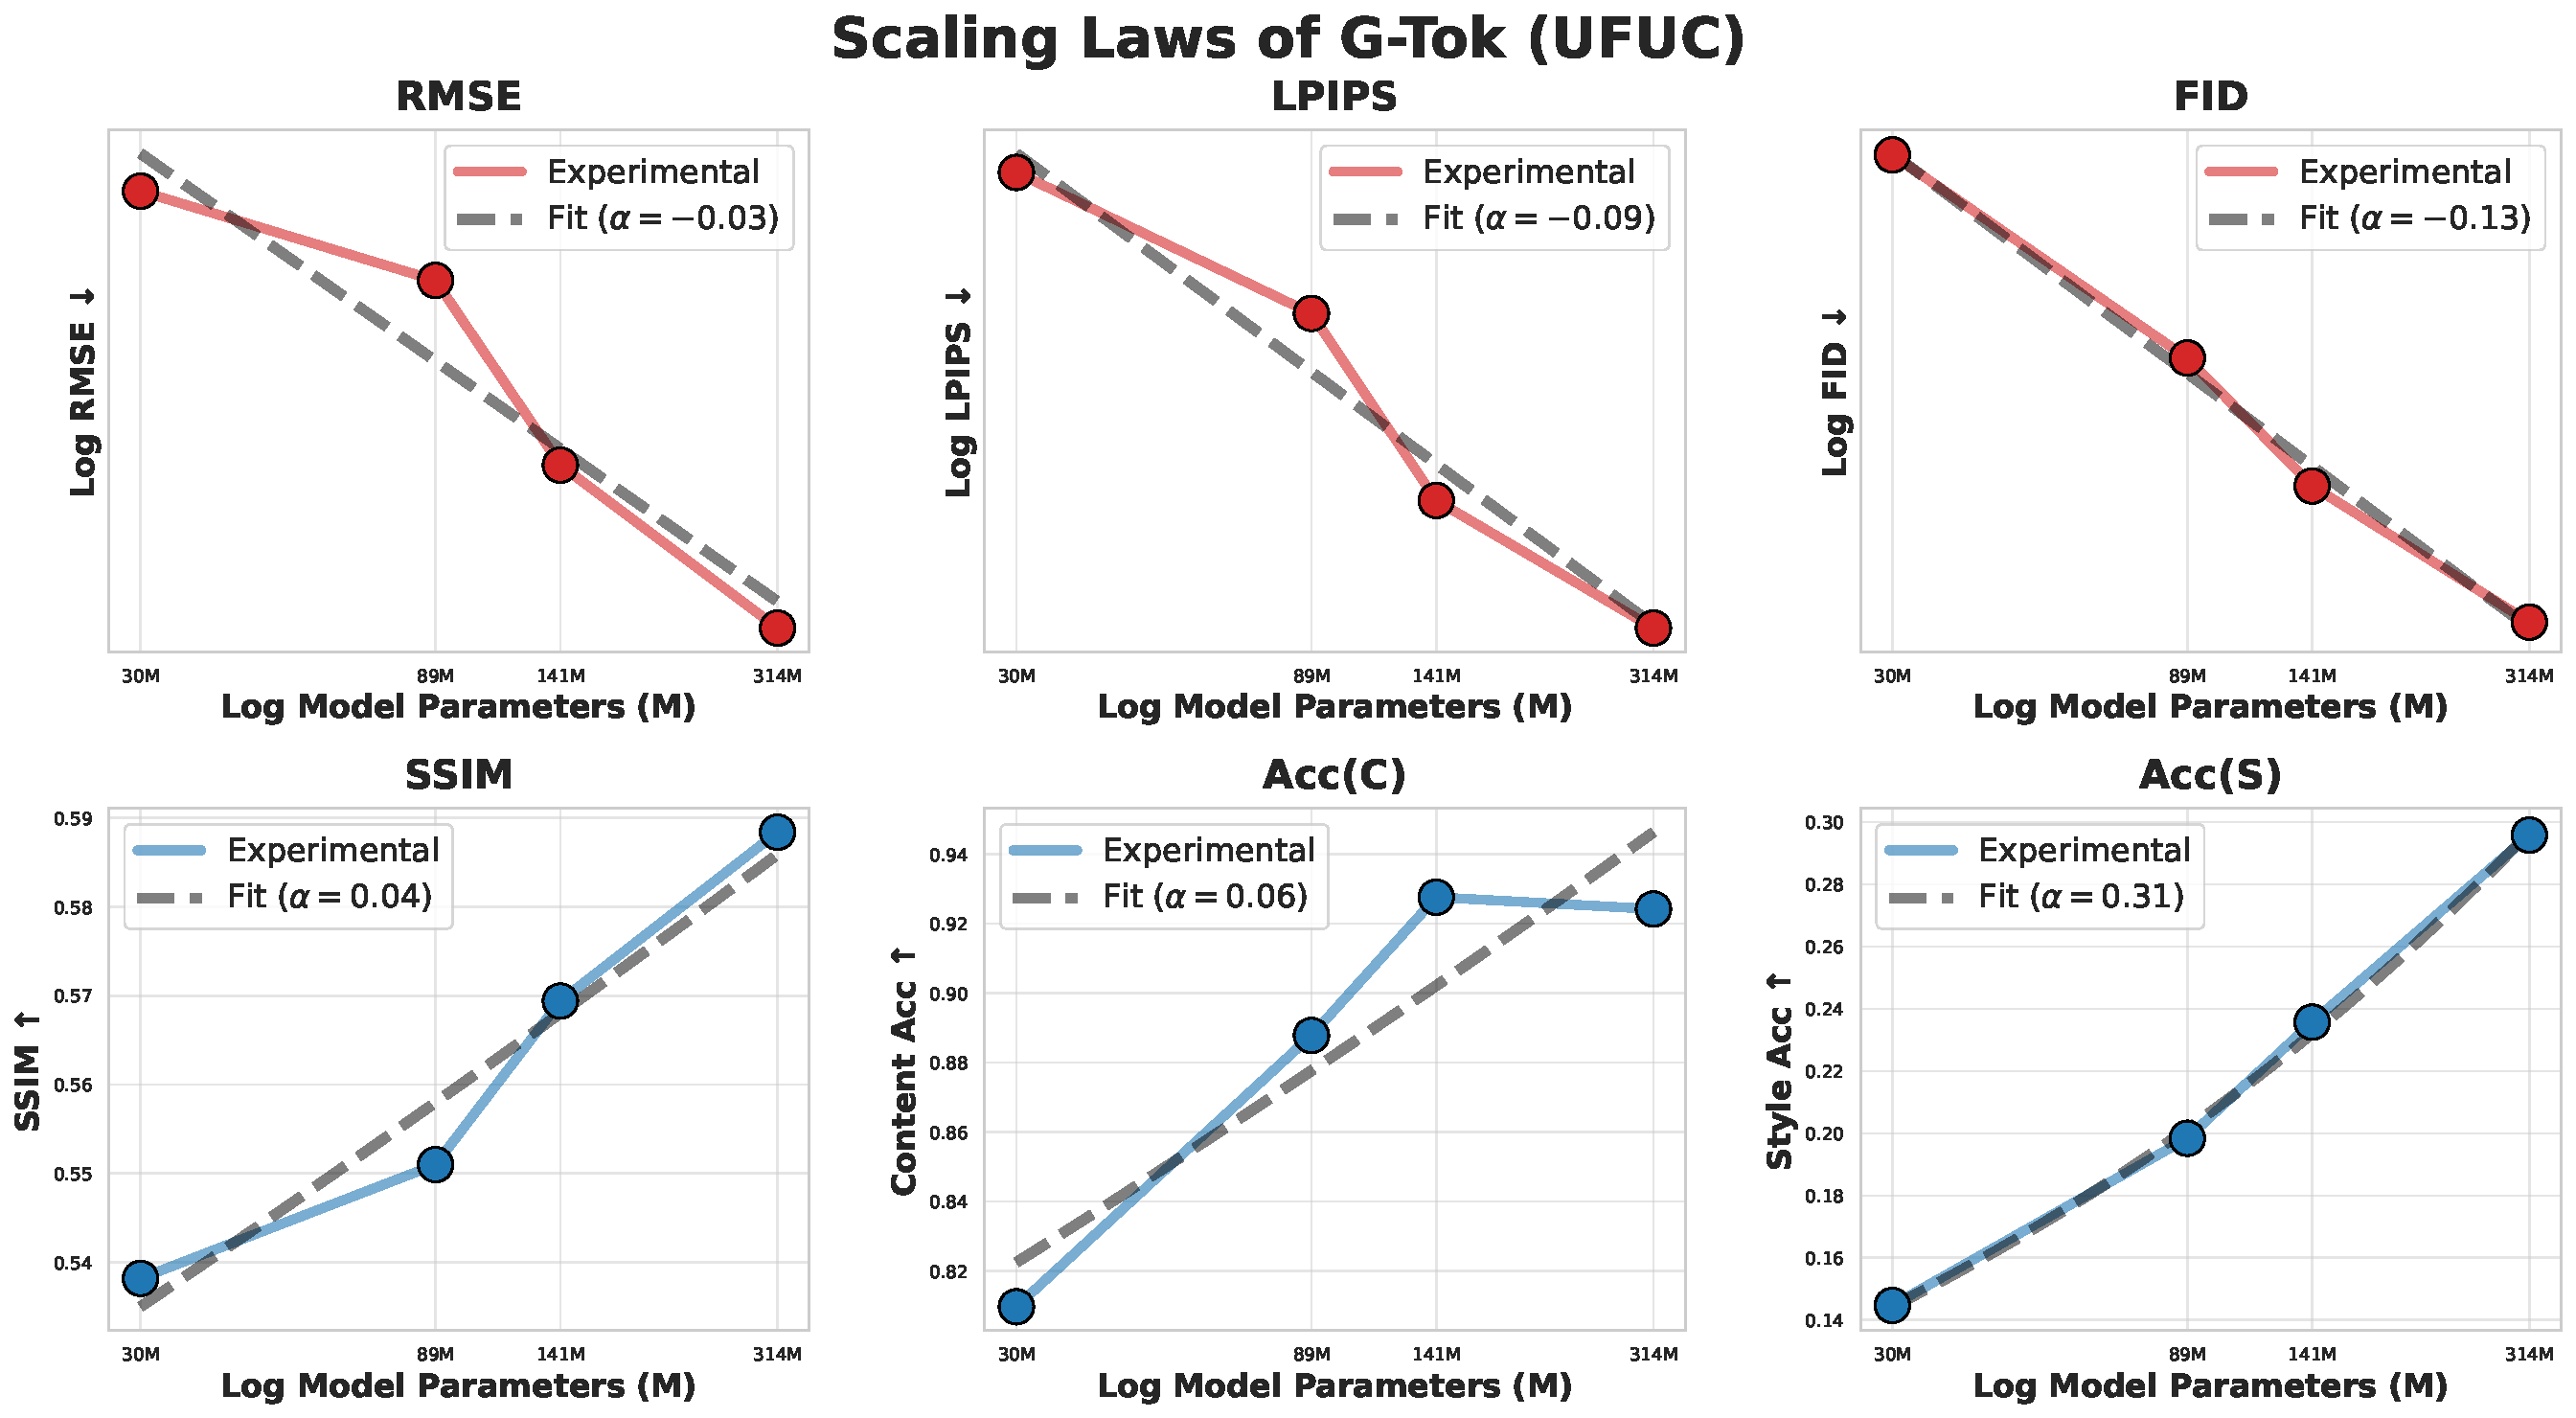
\includegraphics[width=\linewidth]{SUPP_IMGS/scaling_law_UFUC.pdf}
    \end{minipage}
    \vspace{-3mm}
    \caption{Scaling laws of the GAR-Font $(I_8)$ generator with NFA and SE refinement. The plots show performance metrics across model sizes (30M, 89M, 141M, 314M) on Unseen Fonts Seen Characters (\textit{UFSC}) and Unseen Fonts Unseen Characters (\textit{UFUC}). The dashed lines represent power-law fits, highlighting the predictable improvements in both perceptual quality and style generalization.}
    \vspace{-3mm}
    \label{fig:scaling_laws}
\end{figure*}
\subsection{Adaptation on G-Tok to Other FFG Methods}
\label{ssec:quantitiative_G-Tok_plugin}
To verify the versatility of our G-Tok, we integrated it into VQ-Font by replacing its native VQ-VAE with our G-Tok while maintaining the original model architecture and configuration. The modified model, \textbf{VQ-Font (G)}, was trained on the Small dataset with G-Tok. Due to time constraints, we trained it for only 150k iterations, compared with the 500k iterations used in the original VQ-Font. As shown in Table~\ref{tab:quant_eval_gtok_adaptation}, even under shorter training, this simple replacement yields significant improvements across all metrics. Most notably, FID$\downarrow$ decreases by nearly 50\% (e.g., $35.25 \to 17.33$ on \textit{UFSC}) and Content Accuracy$\uparrow$ improves by approximately 9\% ($\sim87\% \to \sim96\%$). These substantial gains demonstrate that G-Tok's hybrid CNN-ViT architecture captures far richer structural and stylistic semantics than standard VQ-VAEs, serving as a robust plug-and-play enhancement for quantization-based FFG methods. Figure~\ref{fig:supple_vq_g_ufuc} illustrates that integrating G-Tok helps the model preserve coherent global structures for complex fonts and generate styles that better align with the target font, indicating a richer and more semantically stable global representation G-Tok than the original VQ-VAE.


\subsection{Post-Refinement of Multimodal FFG}
\label{ssec:mm_post_refinement}

\begin{table*}[!t]
\centering
\caption{Quantitative evaluation of G-Tok's architecture on Unseen Fonts. All models listed are pre-trained on the Small dataset.}
\vspace{-2mm}
\setlength{\tabcolsep}{3pt}
\renewcommand{\arraystretch}{1.05}
\resizebox{0.95\textwidth}{!}{
\begin{tabular}{l | c c c c c c | c c c c c c }
\toprule
Method & \multicolumn{6}{c|}{Unseen Fonts Seen Characters (UFSC)} & \multicolumn{6}{c}{Unseen Fonts Unseen Characters (UFUC)} \\
\cmidrule(lr){2-7} \cmidrule(lr){8-13}
 & RMSE$\downarrow$ & SSIM$\uparrow$ & LPIPS$\downarrow$ & FID$\downarrow$ & Acc(C)$\uparrow$ & Acc(S)$\uparrow$ 
 & RMSE$\downarrow$ & SSIM$\uparrow$ & LPIPS$\downarrow$ & FID$\downarrow$ & Acc(C)$\uparrow$ & Acc(S)$\uparrow$ \\
\hline
CNN & 0.3212 & 0.4836 & 0.1442 & 9.5071 & 0.9051 & 0.0235 & 0.3447 & 0.4350 & 0.1728 & 10.5239 & 0.6722 & 0.0221 \\
CNN+Non-Causal ViT & 0.3183 & 0.4919 & 0.1458 & \textbf{7.9101} & 0.9268 & 0.0402 & 0.3271 & 0.4745 & 0.1562 & 8.7504 & 0.8019 & 0.0436 \\
CNN+Causal ViT & \textbf{0.3080} & \textbf{0.5052} & \textbf{0.1313} & 7.9484 & \textbf{0.9408} & \textbf{0.0802} & \textbf{0.3142} & \textbf{0.4932} & \textbf{0.1421} & \textbf{8.4841} & \textbf{0.8993} & \textbf{0.0796} \\
\bottomrule
\end{tabular}
}
\label{tab:ablation_gtok_generator}
\end{table*}

In Section 4.4, we demonstrated the efficacy of G-Tok$(M_2/M_4)$ on multimodal FFG, but limited to pretraining stage. To fully assess the potential of our lightweight vision-language adaptation, we extend the evaluation to the complete pipeline. We apply our post-training NFA and SE stages to both the vision-only baselines and our multimodal variants. All models are trained on the Large (\textit{L}) dataset.

As visualized in Table~\ref{tab:quant_eval_ref_mm}, the inclusion of textual descriptions significantly enhances the effectiveness of the post-refinement stage. Unlike the pre-training phase where multimodal models showed a slight dip in style accuracy (Acc(S)$\uparrow$), the fully refined GAR-Font($M_2$) and GAR-Font($M_4$) exhibit a substantial lead in Acc(S)$\uparrow$ compared to their vision-only counterparts ($n_\text{ref}=2$ and $n_\text{ref}=4$). Notably, \textbf{GAR-Font($M_4$) outperforms the 8-reference vision-only baseline ($n_\text{ref}=8$)} across most key metrics, including RMSE$\downarrow$, SSIM$\uparrow$, LPIPS$\downarrow$, and Style Accuracy$\uparrow$ (0.4566 vs. 0.4154 on \textit{UFSC}).


\subsection{Scaling Laws of GAR-Font\texorpdfstring{$(I_8)$}{(I8)}}
\label{ssec:scaling_law}
We evaluate the scalability of GAR-Font$(I_8)$ with NFA and SE on the small dataset by training models from 30M to 314M parameters and measuring performance across standard quantitative metrics. Following established scaling-law formulations, we model the relationship between model size $N$ and loss metric $L$ using a power law $L(N)\propto N^{-\alpha}$, and analyze trends in log–log space, where an ideal scaling law appears linear and the slope $\alpha$ reflects scaling efficiency.

As shown in Figure~\ref{fig:scaling_laws}, the enhanced GAR-Font models closely follow these power-law predictions, exhibiting smooth, monotonic improvements across all metrics. Loss-based metrics (FID$\downarrow$, LPIPS$\downarrow$, RMSE$\downarrow$) scale linearly with negative slopes, with FID$\downarrow$ showing a pronounced gain, indicating that larger models continue to yield substantial perceptual improvements without saturation. Accuracy metrics display complementary behavior: Content Accuracy (Acc(C)$\uparrow$) saturates early due to task simplicity, whereas Style Accuracy (Acc(S)$\uparrow$) benefits most from increased capacity. This steep scaling trend highlights that NFA and SE effectively exploit larger parameter budgets to capture and generalize complex stylistic attributes, underscoring the central role of scale in high-fidelity font generation.





% \subsection{Post-Refinement of GAR-Font\texorpdfstring{$(M_2/M_4)$}{(M2/M4)}}

% To fully explore the potential of our lightweight language-style adaptation, we apply the complete post-refinement pipeline (NFA and SE) to GAR-Font($M_2$) and GAR-Font($M_4$). 

% \begin{table*}[t]
% \centering
% \caption{Quantitative evaluation on unseen fonts (MM Post-Refinement train on Large).}
% \vspace{-2mm}
% \setlength{\tabcolsep}{3pt}
% \renewcommand{\arraystretch}{1.05}
% \resizebox{0.95\textwidth}{!}{
% \begin{tabular}{l | c c c c c c | c c c c c c }
% \toprule
% Method & \multicolumn{6}{c|}{Unseen Fonts Seen Characters (UFSC)} & \multicolumn{6}{c}{Unseen Fonts Unseen Characters (UFUC)} \\
% \cmidrule(lr){2-7} \cmidrule(lr){8-13}
%  & RMSE$\downarrow$ & SSIM$\uparrow$ & LPIPS$\downarrow$ & FID$\downarrow$ & Acc(C)$\uparrow$ & Acc(S)$\uparrow$
%  & RMSE$\downarrow$ & SSIM$\uparrow$ & LPIPS$\downarrow$ & FID$\downarrow$ & Acc(C)$\uparrow$ & Acc(S)$\uparrow$ \\
% \hline
% I8\_NFA\_SE\_ref2   & 0.2501 & 0.6438 & 0.0888 & 10.1464 & \textbf{0.9851} & 0.3314 & 0.2701 & 0.5987 & 0.1069 & 9.4294 & 0.8720 & 0.3433 \\
% I8\_NFA\_SE\_ref4   & 0.2437 & 0.6552 & 0.0848 & 9.5960  & 0.9839 & 0.3711 & 0.2692 & 0.6007 & 0.1049 & 9.0877 & 0.8828 & 0.3835 \\
% I8\_NFA\_SE\_ref8   & 0.2398 & 0.6627 & 0.0831 & \textbf{8.3751}  & 0.9776 & 0.4154 & \textbf{0.2508} & \textbf{0.6377} & \textbf{0.0908} & \textbf{7.2034} & \textbf{0.9068} & 0.4183 \\
% MM2\_NFA\_SE        & 0.2361 & 0.6707 & 0.0799 & 8.8867  & 0.9817 & 0.4508 & 0.2527 & 0.6352 & 0.0909 & 8.1444 & 0.9029 & 0.4247 \\
% MM4\_NFA\_SE        & \textbf{0.2358} & \textbf{0.6712} & \textbf{0.0796} & 8.8073  & 0.9800 & \textbf{0.4566} & 0.2524 & 0.6353 & 0.0908 & 8.0699 & 0.9023 & \textbf{0.4391} \\
% \bottomrule
% \end{tabular}
% }
% \label{tab:quant_eval_ref_mm}
% \end{table*}
% \begin{table*}[t]
% \centering
% \caption{Quantitative evaluation on unseen fonts (VQ-Font vs VQ-Font (G).}
% \vspace{-2mm}
% \setlength{\tabcolsep}{3pt}
% \renewcommand{\arraystretch}{1.05}
% \resizebox{0.95\textwidth}{!}{
% \begin{tabular}{l | c c c c c c | c c c c c c }
% \toprule
% Method & \multicolumn{6}{c|}{Unseen Fonts Seen Characters (UFSC)} & \multicolumn{6}{c}{Unseen Fonts Unseen Characters (UFUC)} \\
% \cmidrule(lr){2-7} \cmidrule(lr){8-13}
%  & RMSE$\downarrow$ & SSIM$\uparrow$ & LPIPS$\downarrow$ & FID$\downarrow$ & Acc(C)$\uparrow$ & Acc(S)$\uparrow$
%  & RMSE$\downarrow$ & SSIM$\uparrow$ & LPIPS$\downarrow$ & FID$\downarrow$ & Acc(C)$\uparrow$ & Acc(S)$\uparrow$ \\
% \hline
% VQ\_Font & 0.2727 & 0.5642 & 0.1830 & 35.2472 & 0.8763 & 0.0016 & 0.2744 & 0.5616 & 0.1822 & 36.7914 & 0.8882 & 0.0016 \\
% VQ\_Font (G)   & 0.2725 & 0.5644 & 0.1731 & 17.3296  & 0.9646 & 0.0022 & - & - & - & - &- &- \\
% \bottomrule
% \end{tabular}
% }
% \label{tab:quant_eval_ref_mm}
% \end{table*}


% \subsection{Scaling Laws of GAR-Font$(I_8)$}
% 340M, 150M, 90M, 50M
% To explore how model capacity affects autoregressive font generation, we conduct an additional scaling study on the AR Generator using the Small dataset. We train models of varying sizes and evaluate them across the full set of quantitative metrics, reported in Table~S\_X. The results show a consistent monotonic improvement with increasing model size, demonstrating a clear scaling trend for AR-based glyph modeling.
% \begin{table*}[t]
% \centering
% \caption{Quantitative evaluation on unseen fonts. (Scaling Law, Train on Small)}
% \vspace{-2mm}
% \setlength{\tabcolsep}{3pt}
% \renewcommand{\arraystretch}{1.05}
% \resizebox{0.95\textwidth}{!}{
% \begin{tabular}{l | c c c c c c | c c c c c c }
% \toprule
% Method & \multicolumn{6}{c|}{Unseen Fonts Seen Characters (UFSC)} & \multicolumn{6}{c}{Unseen Fonts Unseen Characters (UFUC)} \\
% \cmidrule(lr){2-7} \cmidrule(lr){8-13}
%  & RMSE$\downarrow$ & SSIM$\uparrow$ & LPIPS$\downarrow$ & FID$\downarrow$ & Acc(C)$\uparrow$ & Acc(S)$\uparrow$
%  & RMSE$\downarrow$ & SSIM$\uparrow$ & LPIPS$\downarrow$ & FID$\downarrow$ & Acc(C)$\uparrow$ & Acc(S)$\uparrow$ \\
% \hline
% 50M\_Pre & 0.3234 & 0.4803 & 0.1478 & 9.5682 & 0.9002 & 0.0347 & 0.3233 & 0.4826 & 0.1473 & 9.8740 & 0.8878 & 0.0375 \\
% 90M\_Pre & 0.3219 & 0.4879 & 0.1409 & 7.9230 & 0.9220 & 0.0448 & 0.3212 & 0.4911 & 0.1409 & 8.1393 & 0.9094 & 0.0502 \\
% 150M\_Pre & 0.3212 & 0.4845 & 0.1449 & 7.9945 & 0.9297 & 0.0471 & 0.3210 & 0.4864 & 0.1449 & 8.4493 & 0.9281 & 0.0506 \\
% 340M\_Pre & 0.3080 & 0.5052 & 0.1313 & 7.9484 & 0.9408 & 0.0802 & 0.3142 & 0.4932 & 0.1421 & 8.4841 & 0.8993 & 0.0796 \\
% \hline
% 50M\_NFA & 0.2977 & 0.5280 & 0.1241 & 10.0811 & 0.7837 & 0.1026 & 0.2979 & 0.5293 & 0.1235 & 10.2685 & 0.7455 & 0.1234 \\
% 90M\_NFA & 0.2937 & 0.5404 & 0.1172 & 7.7879 & 0.8371 & 0.1549 & 0.2928 & 0.5441 & 0.1164 & 7.8355 & 0.8124 & 0.1766 \\
% 150M\_NFA & 0.2874 & 0.5563 & 0.1107 & 6.5190 & 0.8599 & 0.2009 & 0.2862 & 0.5602 & 0.1094 & 6.7234 & 0.8448 & 0.2208 \\
% 340M\_NFA & 0.2712 & 0.5933 & 0.0992 & \textbf{5.4254} & 0.9236 & \textbf{0.3179} & 0.2836 & 0.5702 & 0.1079 & \textbf{5.6667} & 0.8817 & \textbf{0.3277} \\
% \hline
% 50M\_NFA\_SE & 0.2854 & 0.5636 & 0.1148 & 8.9481 & 0.9402 & 0.1330 & 0.2988 & 0.5382 & 0.1257 & 9.6713 & 0.8097 & 0.1447 \\
% 90M\_NFA\_SE & 0.2828 & 0.5732 & 0.1087 & 8.2565 & 0.9649 & 0.1813 & 0.2946 & 0.5510 & 0.1179 & 8.4715 & 0.8878 & 0.1984 \\
% 150M\_NFA\_SE & 0.2760 & 0.5882 & 0.1016 & 7.7190 & 0.9706 & 0.2129 & 0.2861 & 0.5694 & 0.1083 & 7.7930 & 0.9276 & 0.2357 \\
% 340M\_NFA\_SE & \textbf{0.2671} & \textbf{0.6089} & \textbf{0.0948} & 6.9103 & \textbf{0.9718} & 0.2833 & \textbf{0.2788} & \textbf{0.5884} & \textbf{0.1022} & 7.1309 & \textbf{0.9242} & 0.2958 \\
% \bottomrule
% \end{tabular}
% }
% \label{tab:quant_eval_fonts}
% \end{table*}



\section{Additional Ablative Studies}
\label{sec:Ablate}
\subsection{On G-Tok's hybrid Architecture}
% Reconstruction results (0.2 0.2)
To further illustrate the robustness of our hybrid CNN–ViT tokenizer, we provide complete visualizations of the \textbf{Reconstruction Robustness} experiment, where glyphs are corrupted with localized Gaussian noise ($\sigma = 0.2$, affecting 20\% area).  
The qualitative results in Figure~\ref{fig:supple_abl1_rec} demonstrate that G-Tok robustly recovers structural layout and stylistic traits even under severe perturbations, while non-hybrid alternatives fail to reconstruct consistent structure. 

% This visual evidence complements the quantitative robustness results in Section~5.3.

\subsection{On G-Tok's Global and Causal Modeling}
% UFSC,  UFUC,  Small dataset
We present full ablation results for the global and causal modeling components of G-Tok.  
Table ~\ref{tab:ablation_gtok_generator} reports the complete quantitative comparison on the \textit{UFSC/UFUC}. As discussed in Section~5.3, adding global self-attention (CNN + Non-causal ViT) significantly outperforms the CNN-only baseline, while the causal ViT further improves sequential modeling and yields the best overall performance.


Figure ~\ref{fig: supple_abl2_all} provides qualitative comparisons on (\textit{UFSC}, Small) and (\textit{UFUC}, Small). The AR Generator implemented with a CNN-only tokenizer often exhibits style mismatches and inconsistent strokes. Introducing ViT modules into the tokenizer enhances its ability to perceive and capture global stylistic context, leading to more coherent font generation. The AR variant with full G-Tok (CNN + Causal ViT) achieves the most robust performance, showing visible improvements in stylistic and  structural fidelity.

\subsection{On AR Generator's Soft-Decoding}
We provide full visualizations to assess the impact of pixel-level supervision and the soft-decoding strategy. As shown in Figure~\ref{fig: supple_abl3_all} under both (\textit{UFSC}, Small) and (\textit{UFUC}, Small), pixel-level supervision enhances structural accuracy, while soft decoding yields smoother, more continuous strokes and reduces broken segments and visual artifacts.



\begin{figure}[t]
  \centering
  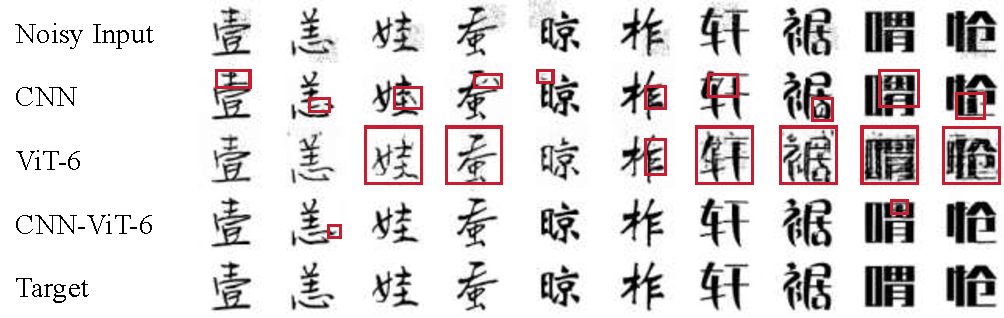
\includegraphics[width=0.95\linewidth]{SUPP_IMGS/EX_Visualization/ABL1_Rec.pdf} 
  \vspace{-3mm}
  \caption{Reconstruction Robustness under localized Gaussian noise ($\sigma = 0.2$, 20\% area). \textcolor{ex2figure_red}{\fbox{\rule{0pt}{4pt}\rule{4pt}{0pt}}} marks structural mistakes. G-Tok maintains structural and stylistic fidelity despite heavy corruption, while non-hybrid tokenizers exhibit unstable and inconsistent reconstructions.}
  \vspace{-3mm}
  \label{fig:supple_abl1_rec}
\end{figure}

\begin{figure*}[tp] % [p] 强制将这些内容放在单独的一页
    \centering
    
    % ================== 第一组图 (G-Tok) ==================
    \begin{subfigure}{0.93\linewidth} % 尝试缩小到 0.8 或 0.75
        \centering
        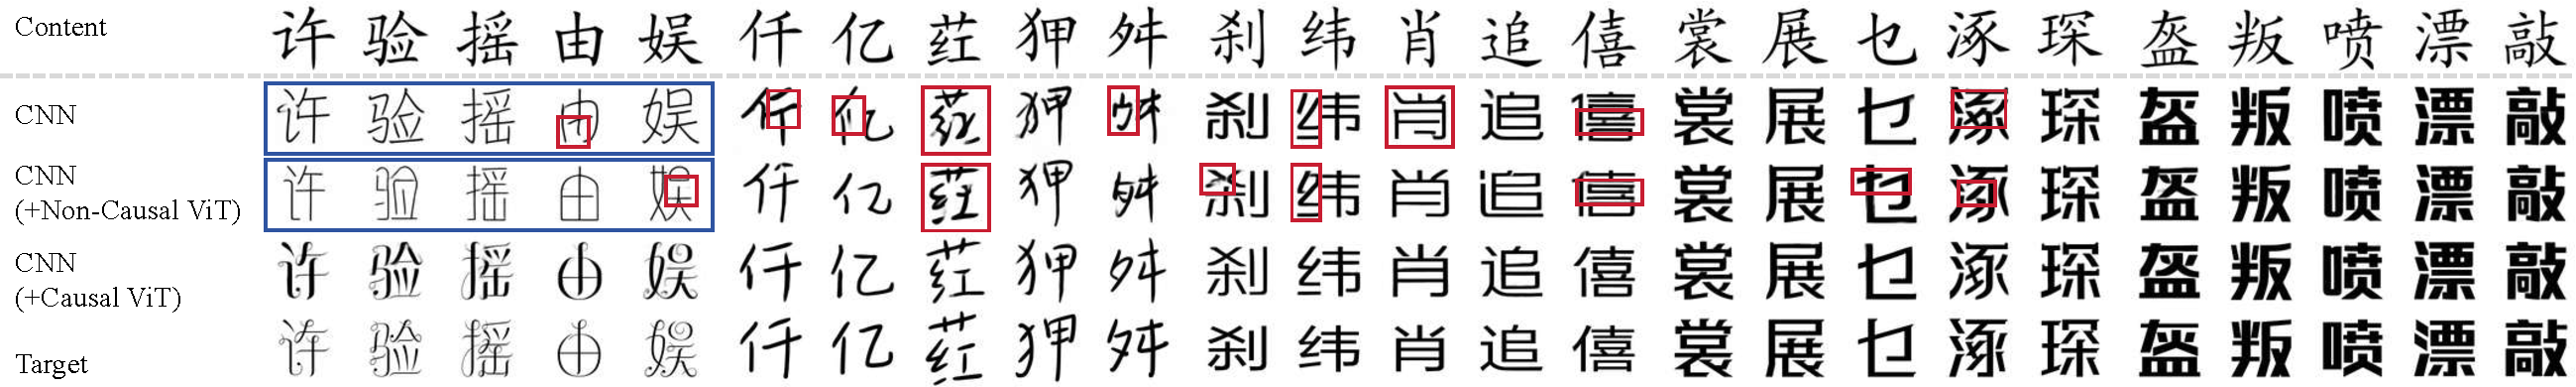
\includegraphics[width=\linewidth]{SUPP_IMGS/EX_Visualization/ABL2_table_UFSC_Small.pdf}
        \caption{\textit{UFSC}, Small dataset}
        \label{fig: supple_abl2_ufsc_small}
    \end{subfigure}
    \\ % 强制换行，确保垂直排列
    \begin{subfigure}{0.93\linewidth}
        \centering
        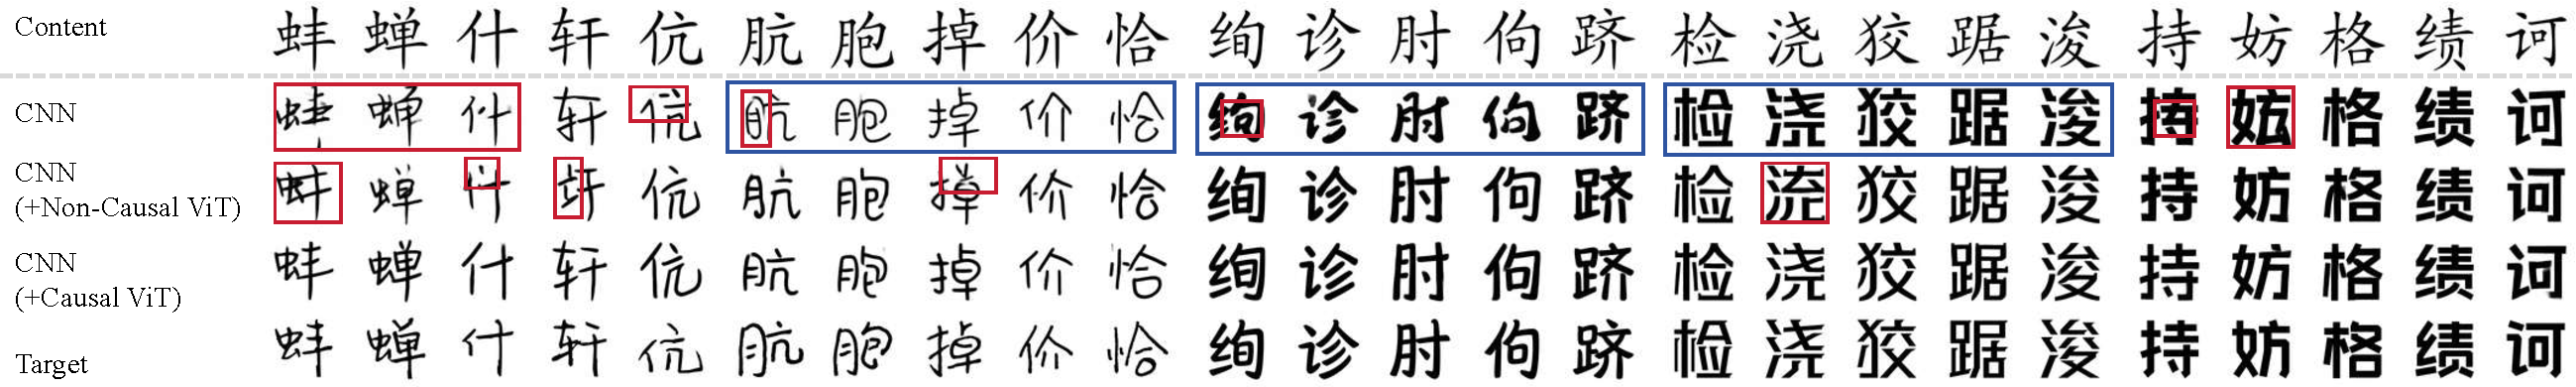
\includegraphics[width=\linewidth]{SUPP_IMGS/EX_Visualization/ABL2_table_UFUC_Small.pdf}
        \caption{\textit{UFUC}, Small dataset}
        \label{fig: supple_abl2_ufuc_small}
    \end{subfigure}
    \vspace{-3mm}
    \caption{Qualitative results on G-Tok's Global and Causal Modeling under \textit{UFSC} and \textit{UFUC} protocols
        (Small dataset). 
        \textcolor{ex1figure_red}{\fbox{\rule{0pt}{4pt}\rule{4pt}{0pt}}} /
        \textcolor{ex1figure_blue}{\fbox{\rule{0pt}{4pt}\rule{4pt}{0pt}}}
        indicate structural errors and style mismatches.}
    \label{fig: supple_abl2_all}
    
    \vspace{1em} % 在不同 Figure 之间增加一点区分距离
    
    % ================== 第二组图 (AR Generator) ==================
    \begin{subfigure}{0.93\linewidth}
        \centering
        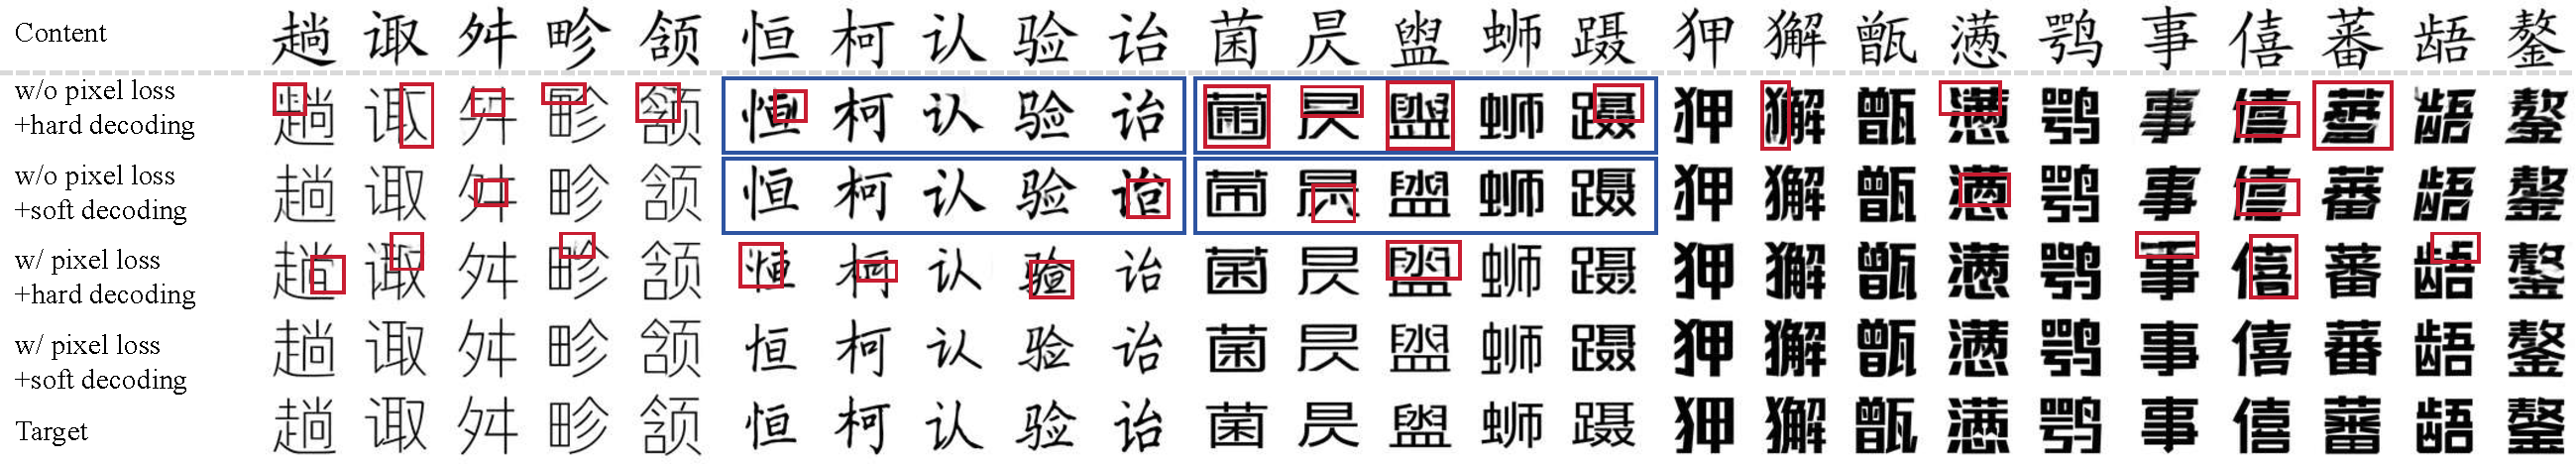
\includegraphics[width=\linewidth]{SUPP_IMGS/EX_Visualization/ABL3_Table_UFSC_Small.pdf}
        \caption{\textit{UFSC}, Small dataset}
        \label{fig: supple_abl3_ufsc_small}
    \end{subfigure}
    \\
    \begin{subfigure}{0.93\linewidth}
        \centering
        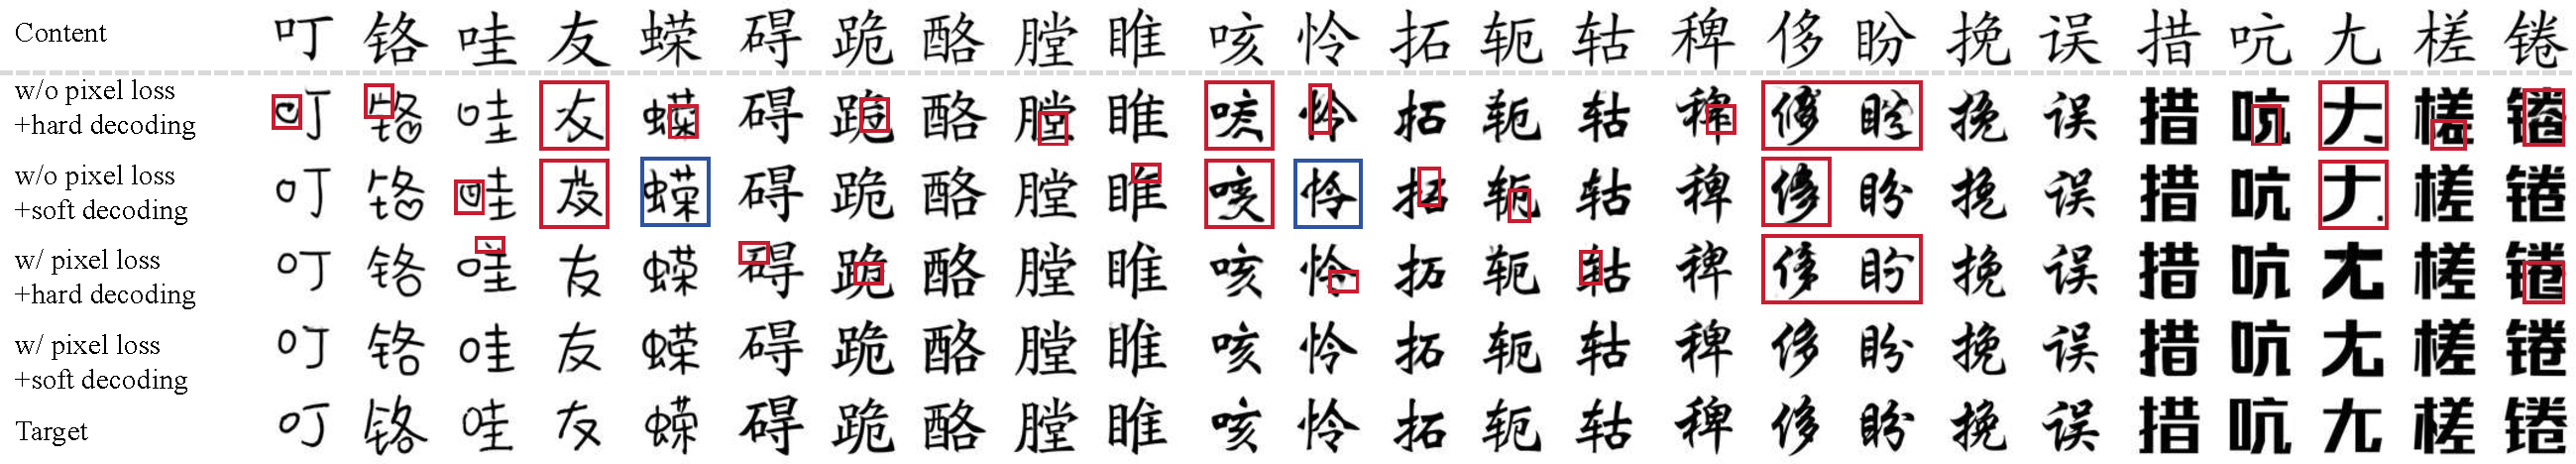
\includegraphics[width=\linewidth]{SUPP_IMGS/EX_Visualization/ABL3_Table_UFUC_Small.pdf}
        \caption{\textit{UFUC}, Small dataset}
        \label{fig: supple_abl3_ufuc_small}
    \end{subfigure}
    \vspace{-3mm}
    \caption{Qualitative results on AR Generator's Soft-decoding under \textit{UFSC} and \textit{UFUC} protocols
        (Small dataset).
        \textcolor{ex1figure_red}{\fbox{\rule{0pt}{4pt}\rule{4pt}{0pt}}} /
        \textcolor{ex1figure_blue}{\fbox{\rule{0pt}{4pt}\rule{4pt}{0pt}}}
        indicate structural errors and style mismatches.}
    \label{fig: supple_abl3_all}

    \vspace{1em}

    % ================== 第三组图 (Multimodal Style) ==================
    \begin{subfigure}{0.93\linewidth}
        \centering
        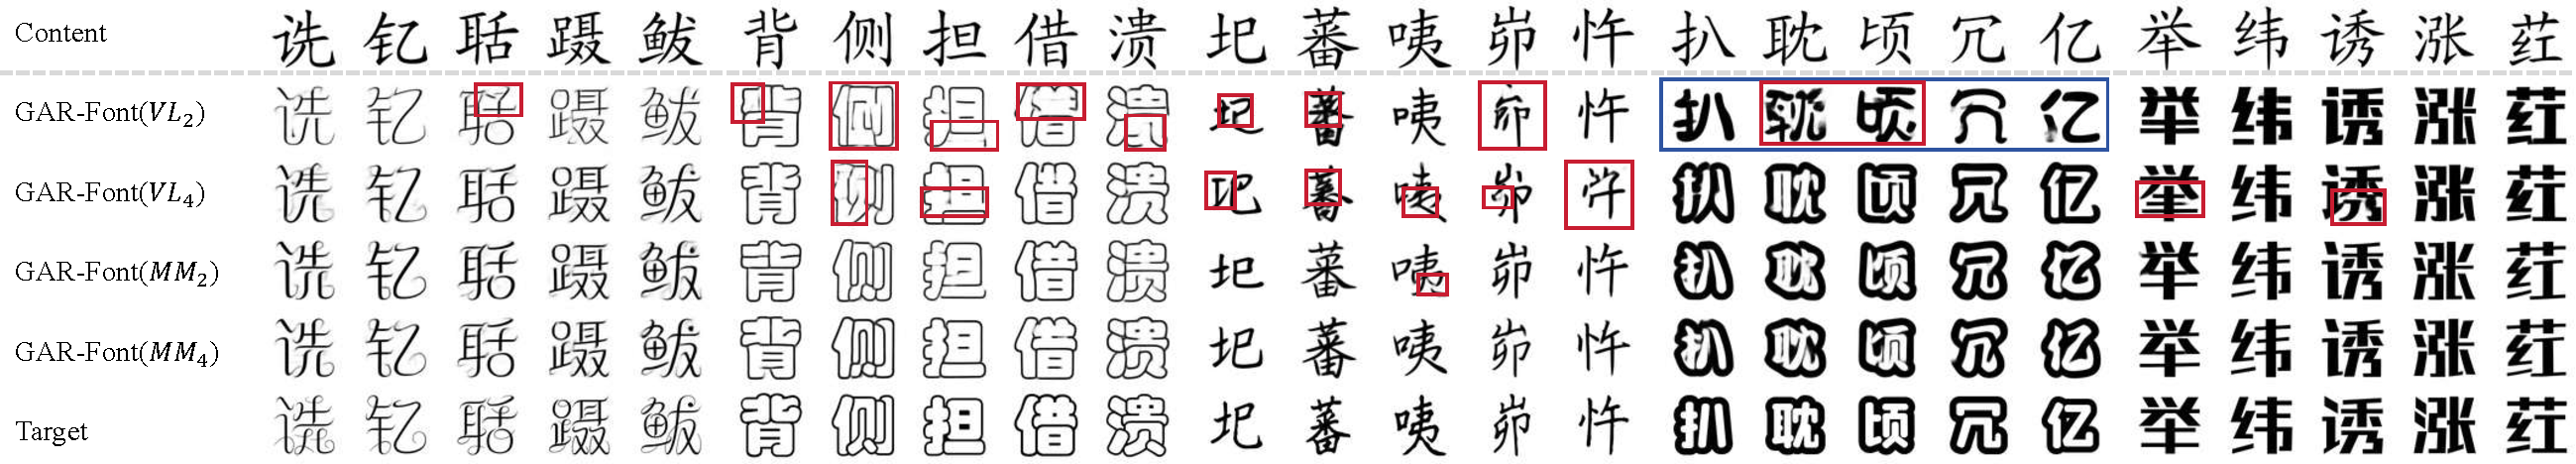
\includegraphics[width=\linewidth]{SUPP_IMGS/EX_Visualization/ABL4_Table_UFSC_Large.pdf}
        \caption{\textit{UFSC}, Large dataset}
        \label{fig: supple_abl4_ufsc_large}
    \end{subfigure}
    \\
    \begin{subfigure}{0.93\linewidth}
        \centering
        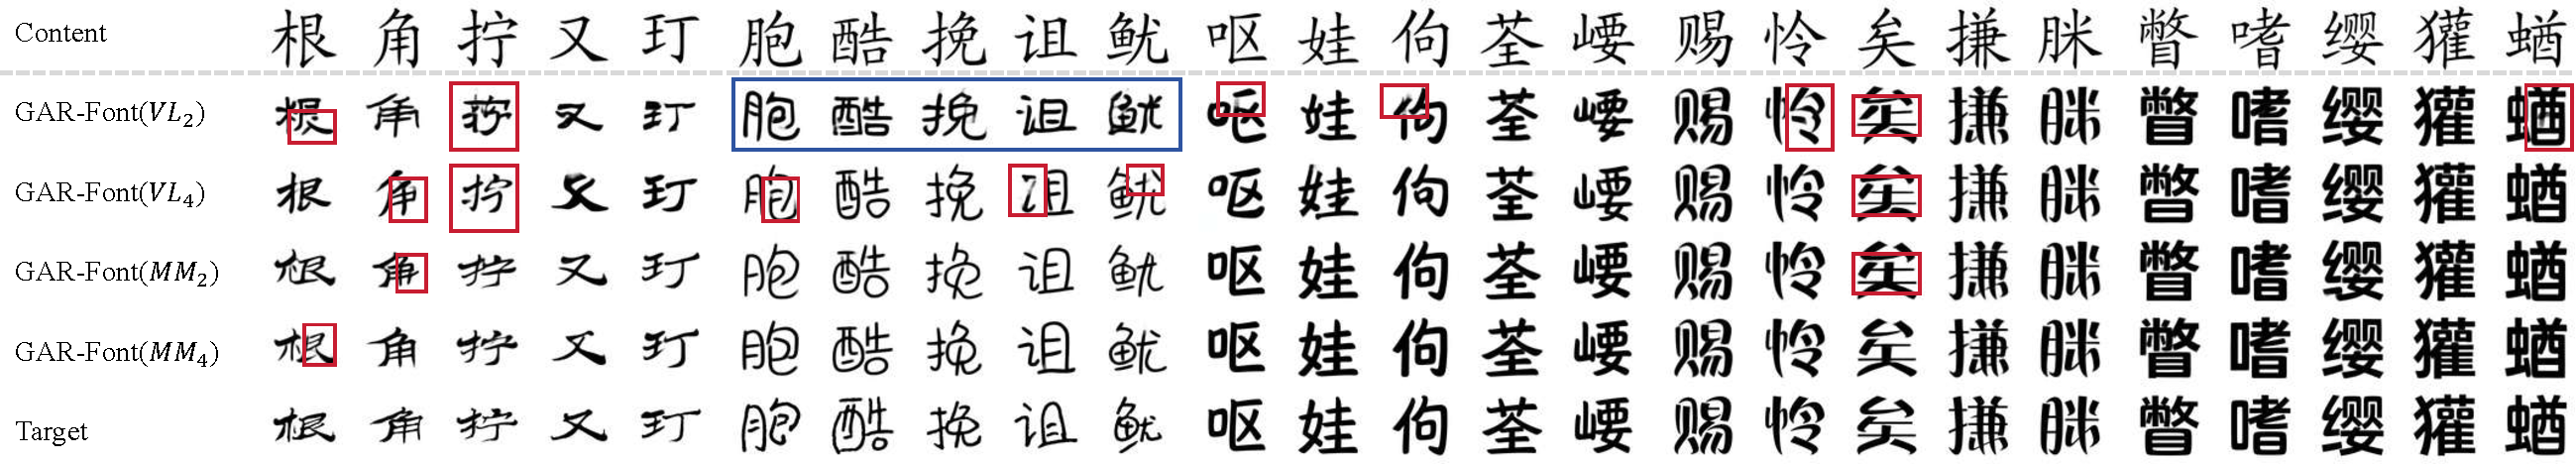
\includegraphics[width=\linewidth]{SUPP_IMGS/EX_Visualization/ABL4_Table_UFUC_Large.pdf}
        \caption{\textit{UFUC}, Large dataset}
        \label{fig: supple_abl4_ufuc_large}
    \end{subfigure}
    \vspace{-3mm}
    \caption{
        Qualitative results on Multimodal Style Encoder's Adaptation under \textit{UFSC} and \textit{UFUC} protocols
        (Large dataset).
        \textcolor{ex1figure_red}{\fbox{\rule{0pt}{4pt}\rule{4pt}{0pt}}} /
        \textcolor{ex1figure_blue}{\fbox{\rule{0pt}{4pt}\rule{4pt}{0pt}}}
        indicate structural errors and style mismatches.
    }
    \label{fig: supple_abl4_all}
    
\end{figure*}
\begin{figure*}[tp]
    \centering

    \begin{subfigure}{0.91\linewidth}
        \centering
        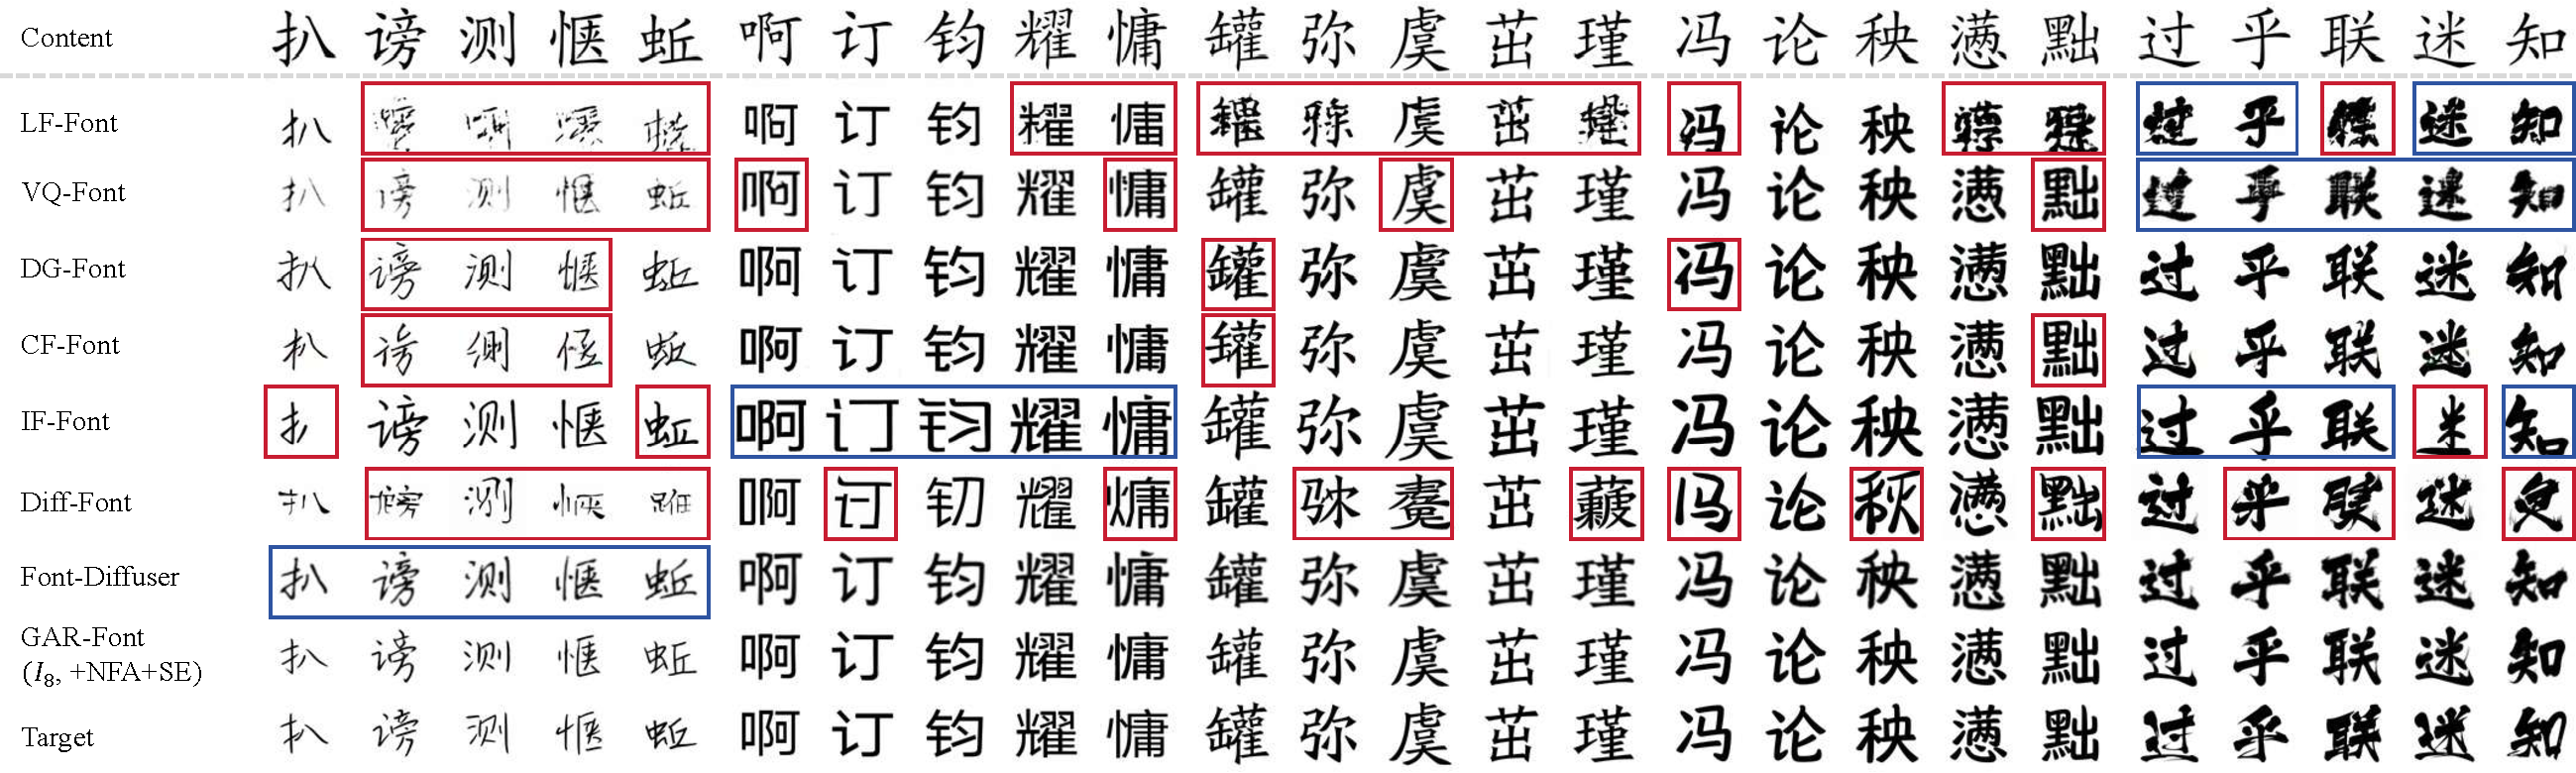
\includegraphics[width=\linewidth]{SUPP_IMGS/EX_Visualization/table_Main1_UFSC_Small.pdf}
        \vspace{-3mm}
        \caption{\textit{UFSC}, Small dataset}
        \label{fig: supple_main1_ufsc_small}
        \vspace{1mm}
    \end{subfigure}

    \begin{subfigure}{0.91\linewidth}
        \centering
        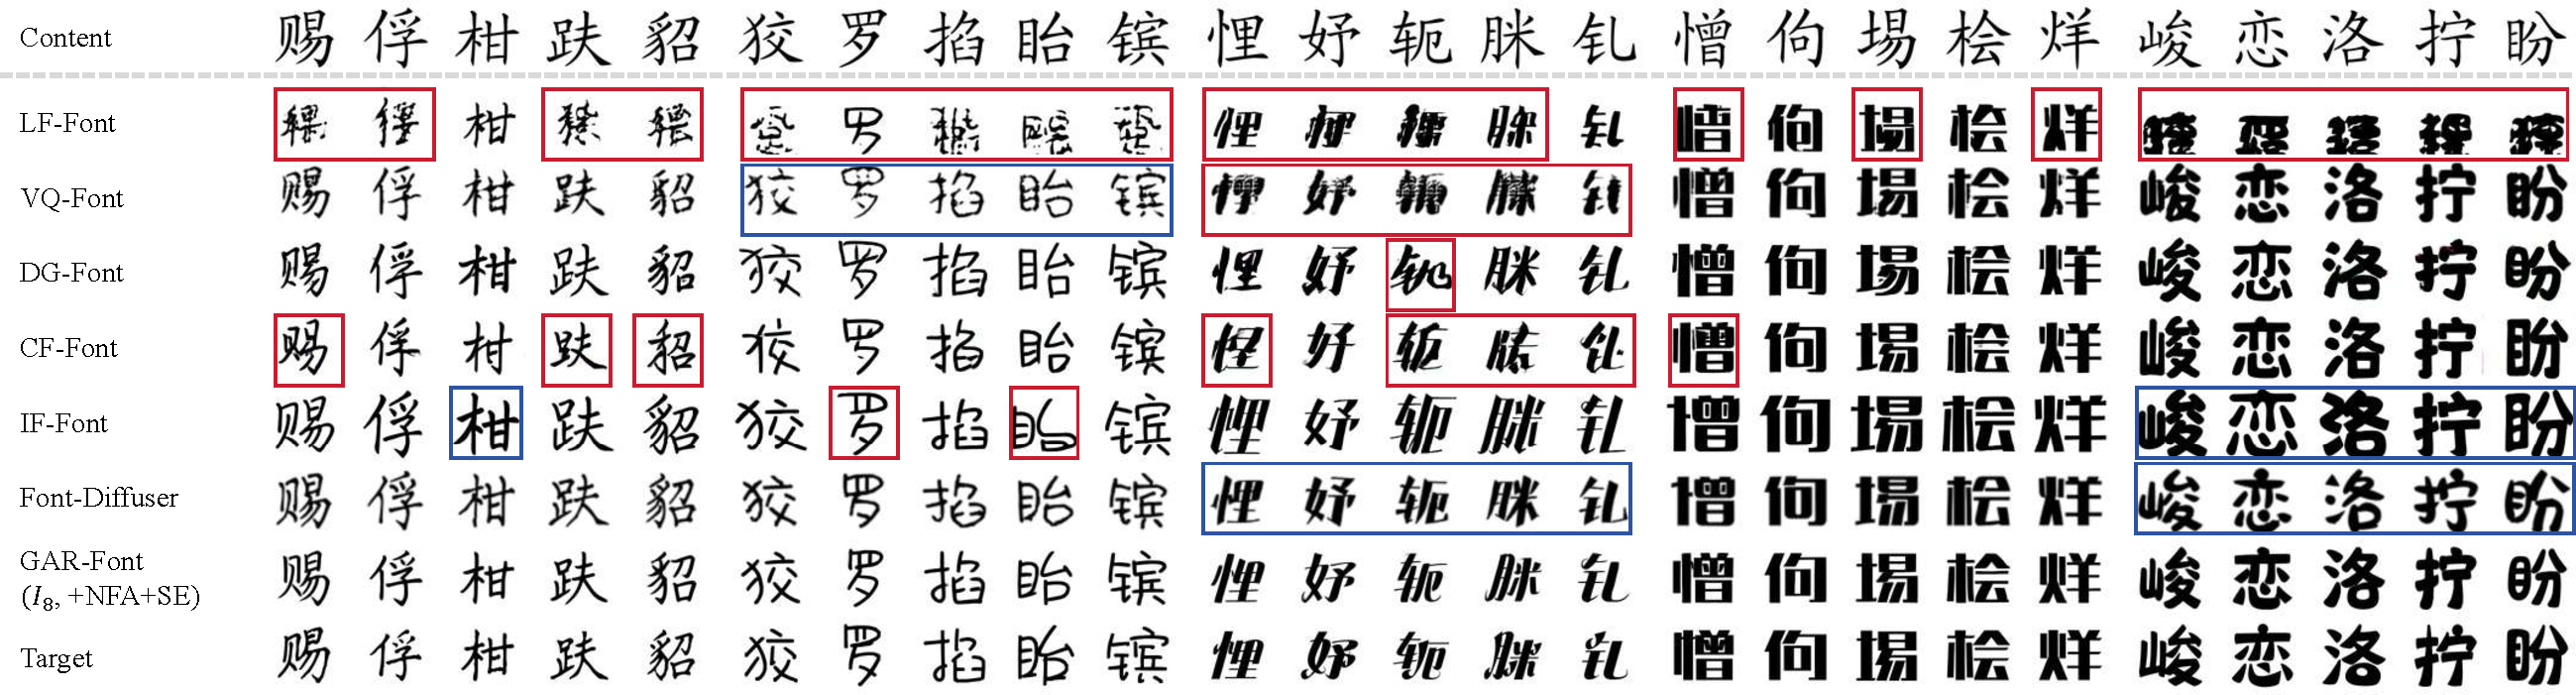
\includegraphics[width=\linewidth]{SUPP_IMGS/EX_Visualization/table_Main1_UFUC_Small.pdf}
        \vspace{-3mm}
        \caption{\textit{UFUC}, Small dataset}
        \vspace{1mm}
        \label{fig: supple_main1_ufuc_small}
    \end{subfigure}

    \begin{subfigure}{0.91\linewidth}
        \centering
        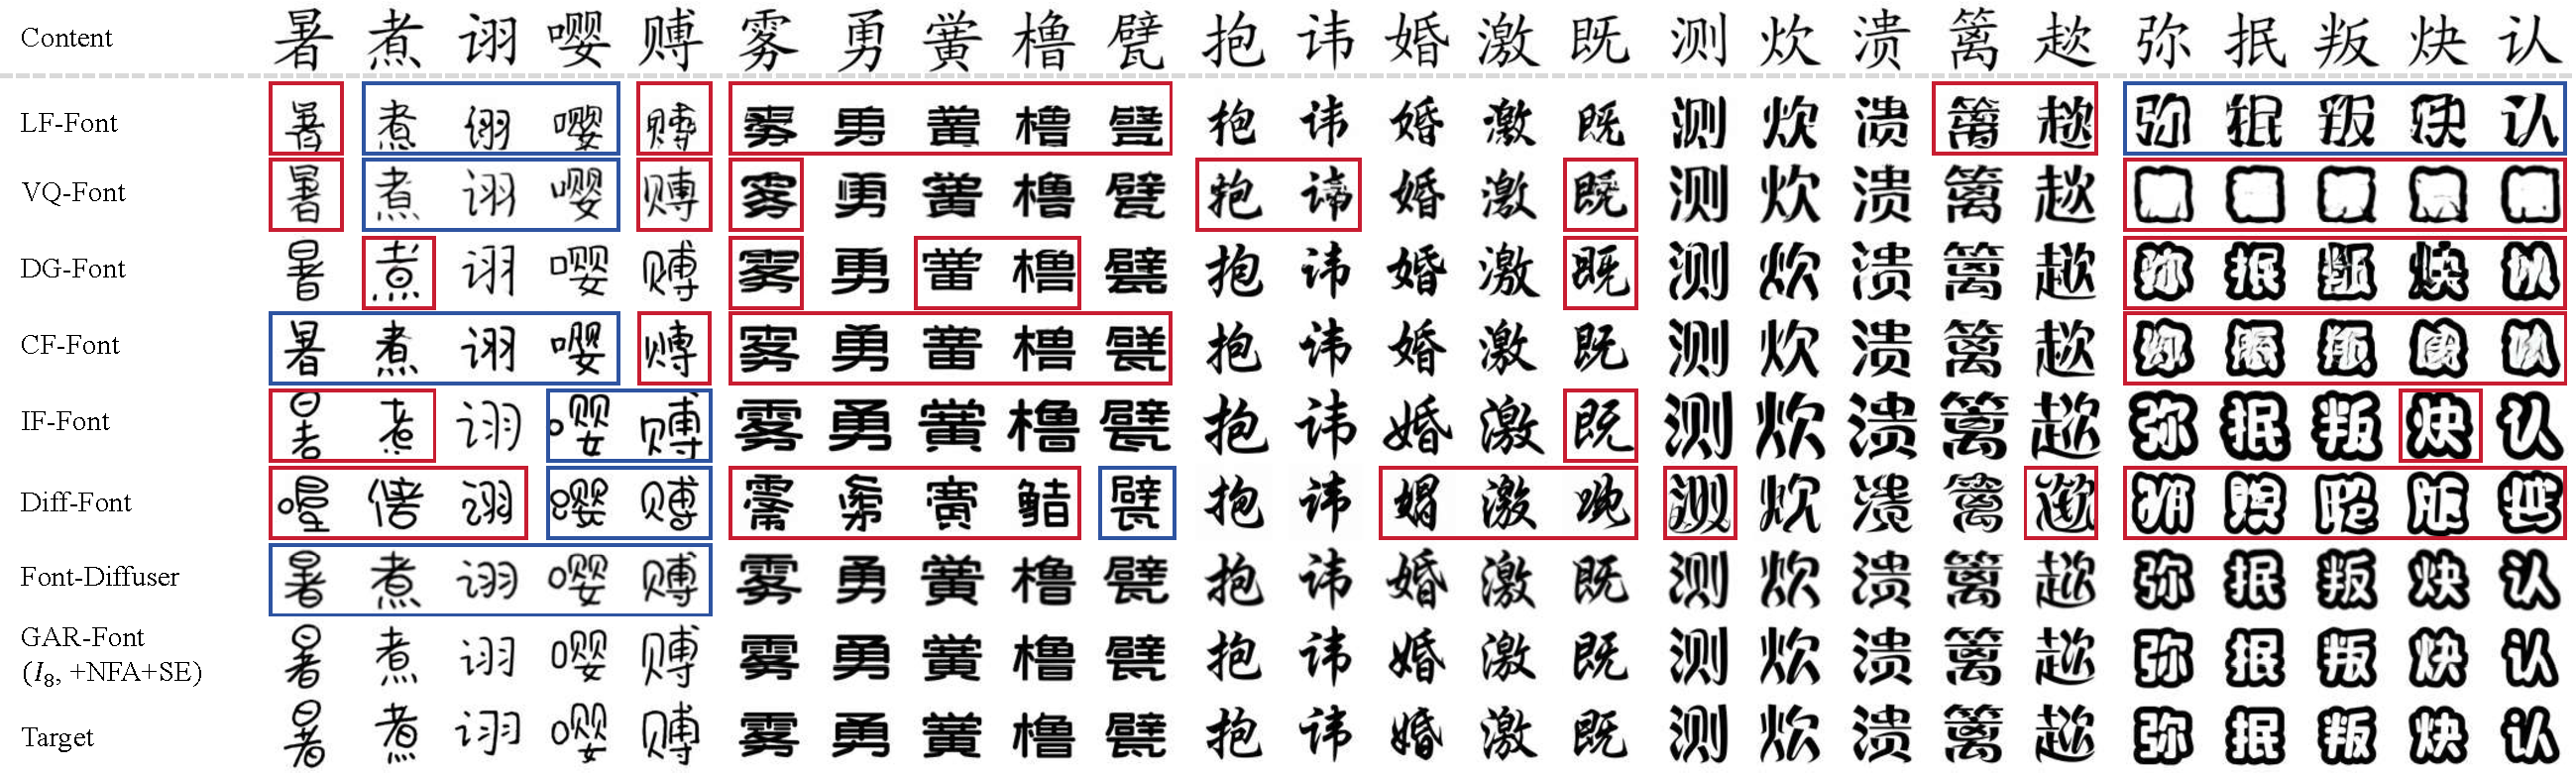
\includegraphics[width=\linewidth]{SUPP_IMGS/EX_Visualization/table_Main1_UFSC_Large.pdf}
        \vspace{-3mm}
        \caption{\textit{UFSC}, Large dataset}
        \vspace{1mm}
        \label{fig: supple_main1_ufsc_large}
    \end{subfigure}

    \begin{subfigure}{0.91\linewidth}
        \centering
        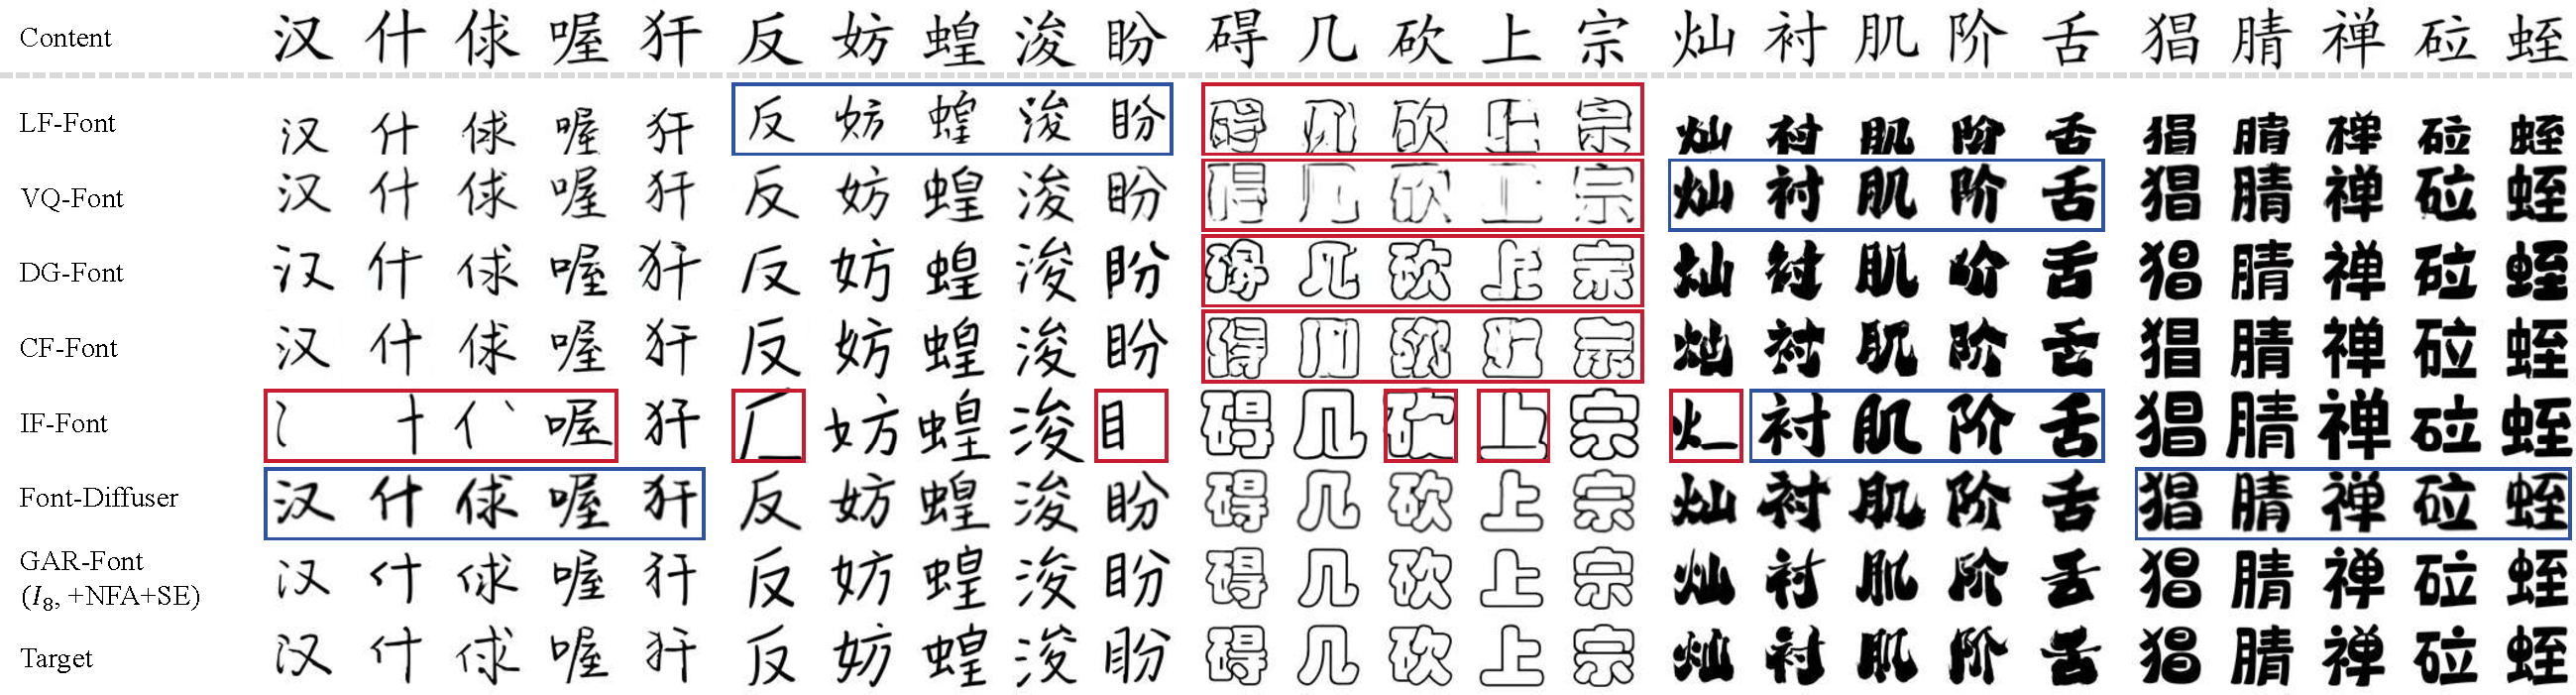
\includegraphics[width=\linewidth]{SUPP_IMGS/EX_Visualization/table_Main1_UFUC_Large.pdf}
        \vspace{-3mm}
        \caption{\textit{UFUC}, Large dataset}
        \vspace{1mm}
        \label{fig: supple_main1_ufuc_large}
    \end{subfigure}
    \vspace{-2mm}
    \caption{
        Qualitative results on vision-only FFG across \textit{UFSC/UFUC} protocols and Small/Large datasets.
        \textcolor{ex1figure_red}{\fbox{\rule{0pt}{4pt}\rule{4pt}{0pt}}} /
        \textcolor{ex1figure_blue}{\fbox{\rule{0pt}{4pt}\rule{4pt}{0pt}}}
        indicate structural errors and style mismatches.
    }
    
    \vspace{-4mm}
    \label{fig: supple_main1_all}
\end{figure*}


\subsection{On Multimodal Style Encoder's Adaptation}
% UFSC,  UFUC,  Large dataset
We compare our decoupled multimodal training paradigm against joint training of the multimodal style encoder. While quantitative results are provided in Section 5.3, we present the full set of qualitative comparisons here.

Figure ~\ref{fig: supple_abl4_all} presents visual comparisons on (\textit{UFSC}, Large) and (\textit{UFUC}, Large). The results reveal that GAR-Font($M_2$/$M_4$), trained with the decoupled training scheme, generate glyphs whose font styles more closely align with the target compared to the jointly trained GAR-Font($VL_2$/$VL_4$). They also demonstrate better character-structure accuracy. The decoupled training strategy enables the model to fully leverage the visual encoder’s representational capacity, thereby preserving fine-grained style features and structural priors that may be harder to retain under joint optimization.


\begin{figure*}[tp] % [p] 强制单独一页
    \centering

    % =========================================
    % 第一组：Pre-Train
    % =========================================
    
    % -------- (a) Pre --------
    \begin{subfigure}{0.92\linewidth} % 建议缩小到 0.9 或 0.85 以防超高
        \centering
        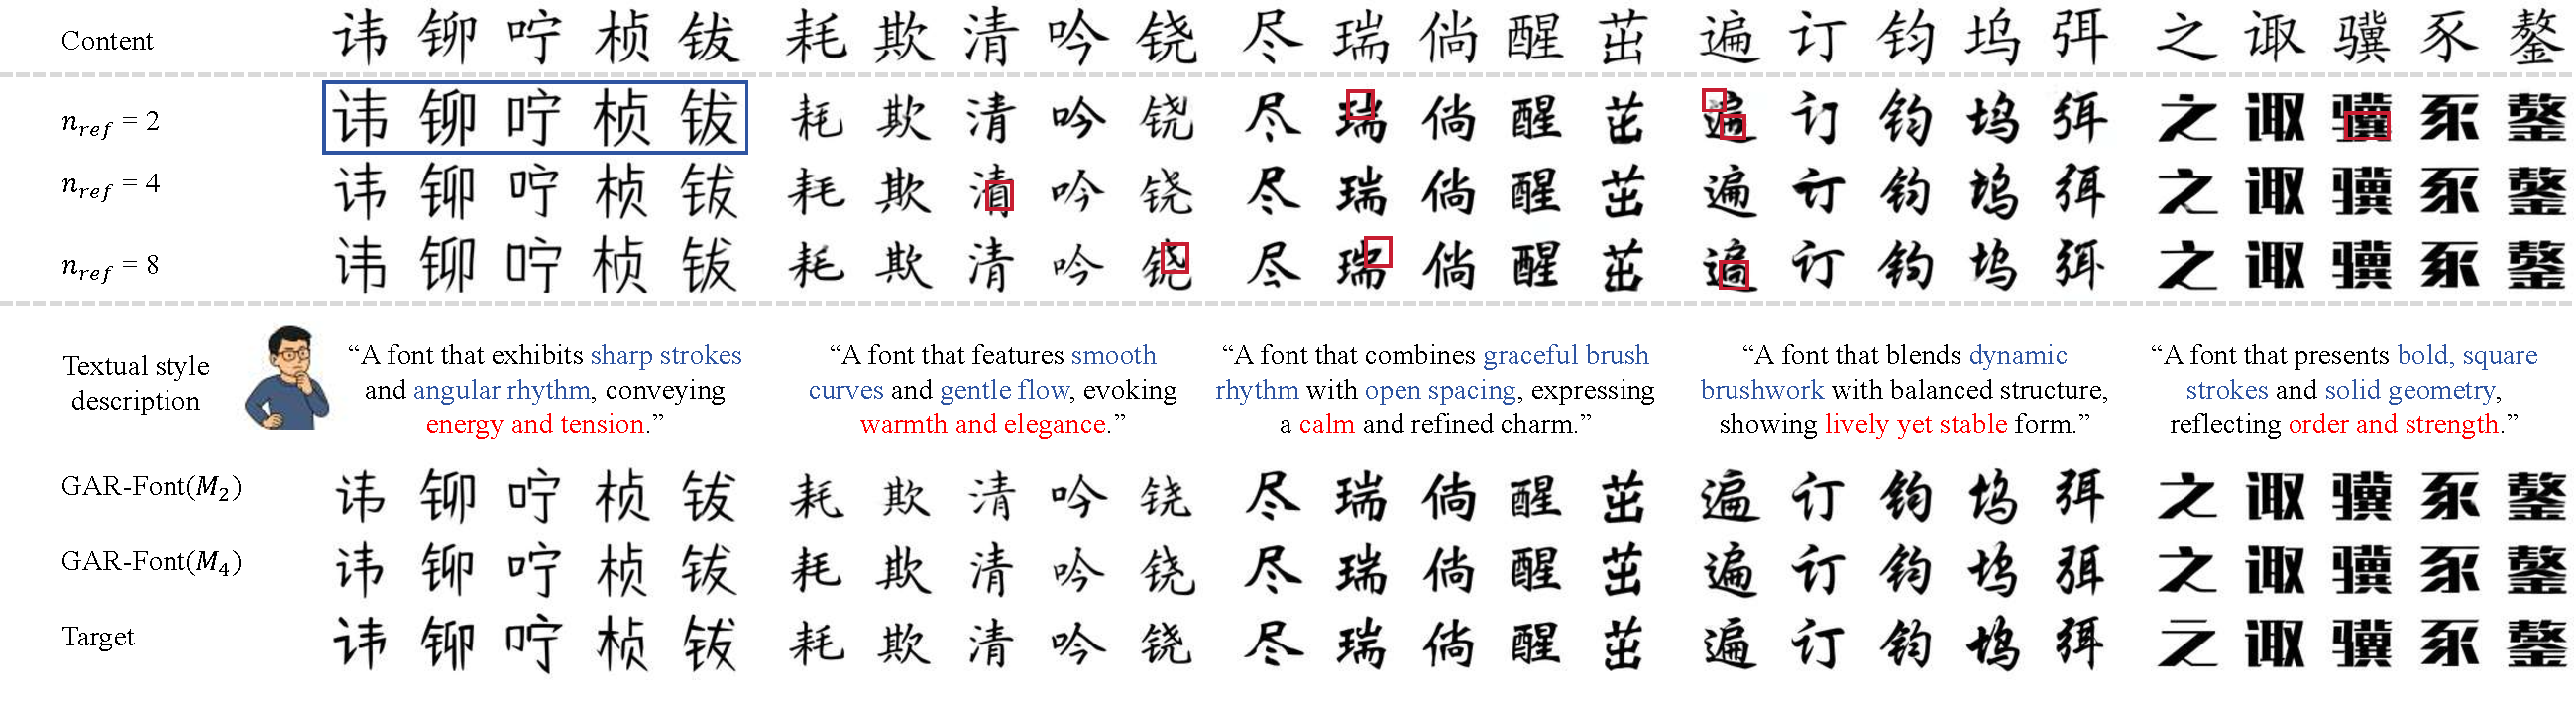
\includegraphics[width=\linewidth]{SUPP_IMGS/EX_Visualization/table2_supple_UFSC_Large_Pre.pdf}
        \caption{\textit{UFSC}, Large dataset}
        \label{fig: supple_main2_ufsc_large_pre}
    \end{subfigure}
    \\ % 强制换行
    \vspace{1mm} % 稍微减少间距
    % -------- (b) Pre --------
    \begin{subfigure}{0.92\linewidth}
        \centering
        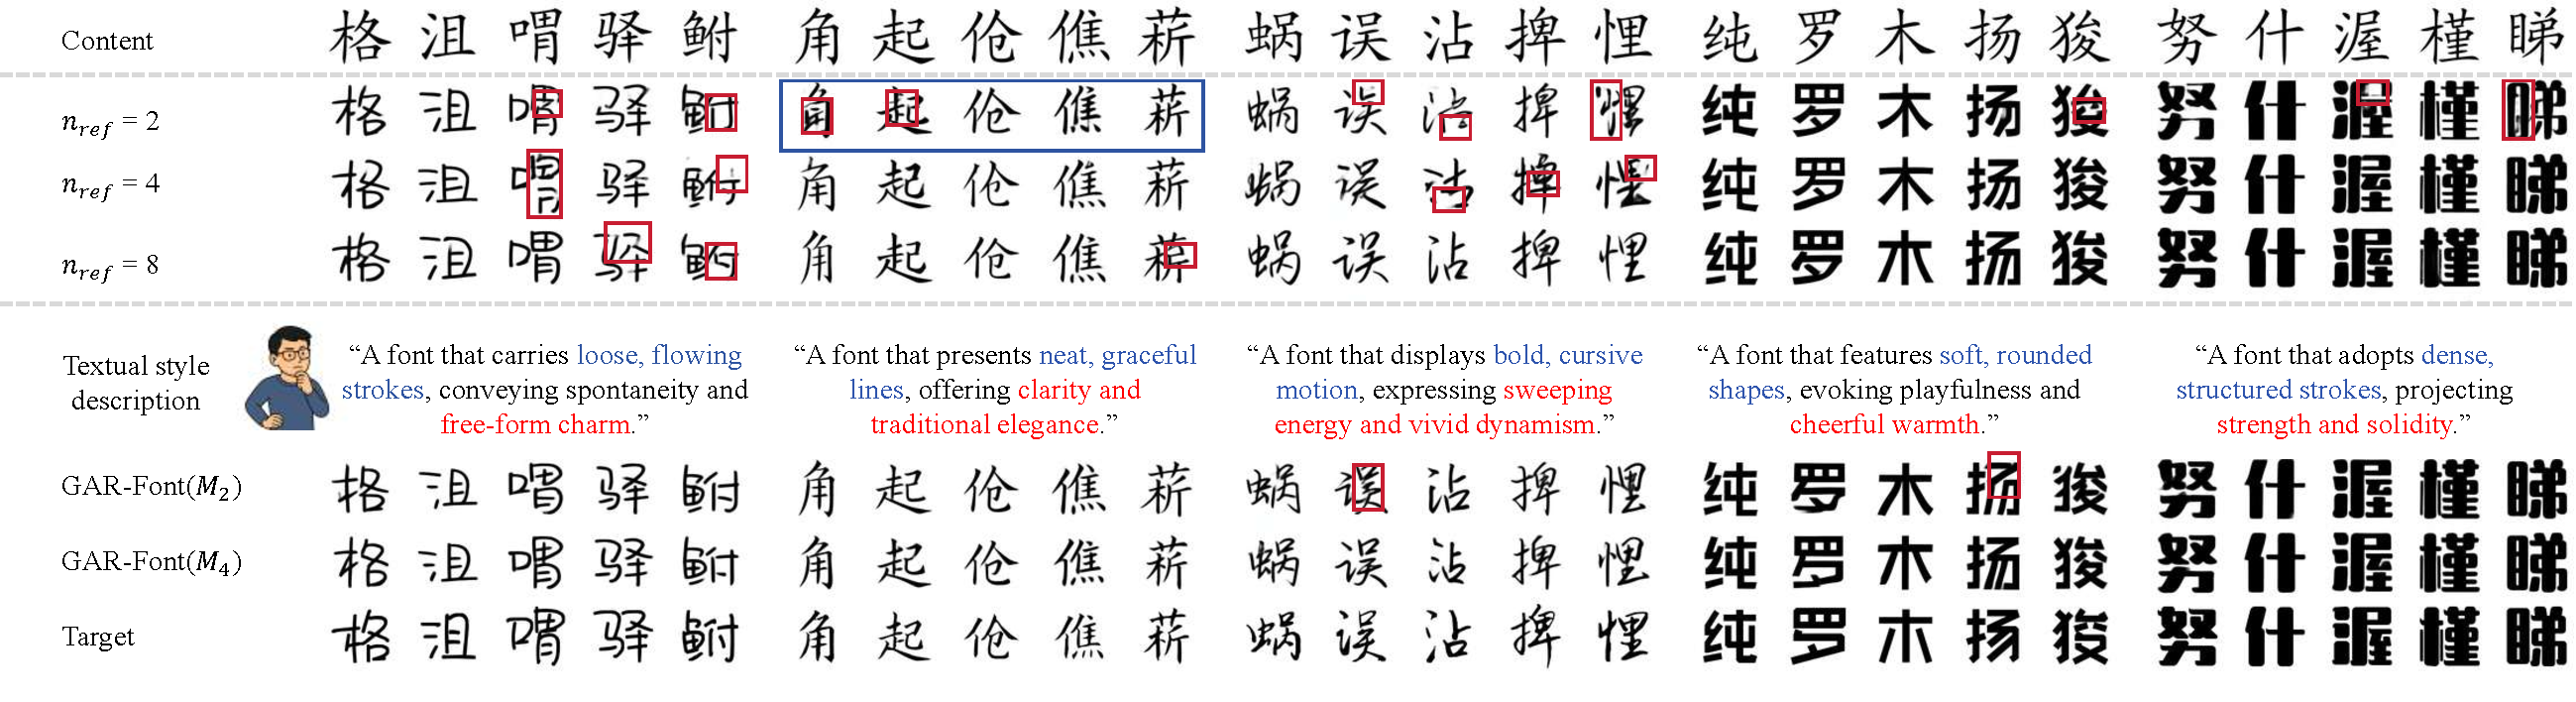
\includegraphics[width=\linewidth]{SUPP_IMGS/EX_Visualization/table2_supple_UFUC_Large_Pre.pdf}
        \caption{\textit{UFUC}, Large dataset}
        \label{fig: supple_main2_ufuc_large_pre}
    \end{subfigure}
    \vspace{-2mm}
    
    % -------- 第一组 Caption --------
    \caption{
        Qualitative results of Pre-Train multimodal FFG under \textit{UFSC} and \textit{UFUC} protocols
        (Large dataset). 
        \textcolor{ex2figure_red}{\fbox{\rule{0pt}{4pt}\rule{4pt}{0pt}}} denotes local slight structural mistakes, 
        and \textcolor{ex2figure_blue}{\fbox{\rule{0pt}{4pt}\rule{4pt}{0pt}}} marks stylistic drift.
    }
    \label{fig: supple_main2_large_pre_all}

    \vspace{1em} % 在两个大图组之间增加明显间距

    % =========================================
    % 第二组：Post-Refine
    % =========================================

    % -------- (a) Post --------
    \begin{subfigure}{0.92\linewidth}
        \centering
        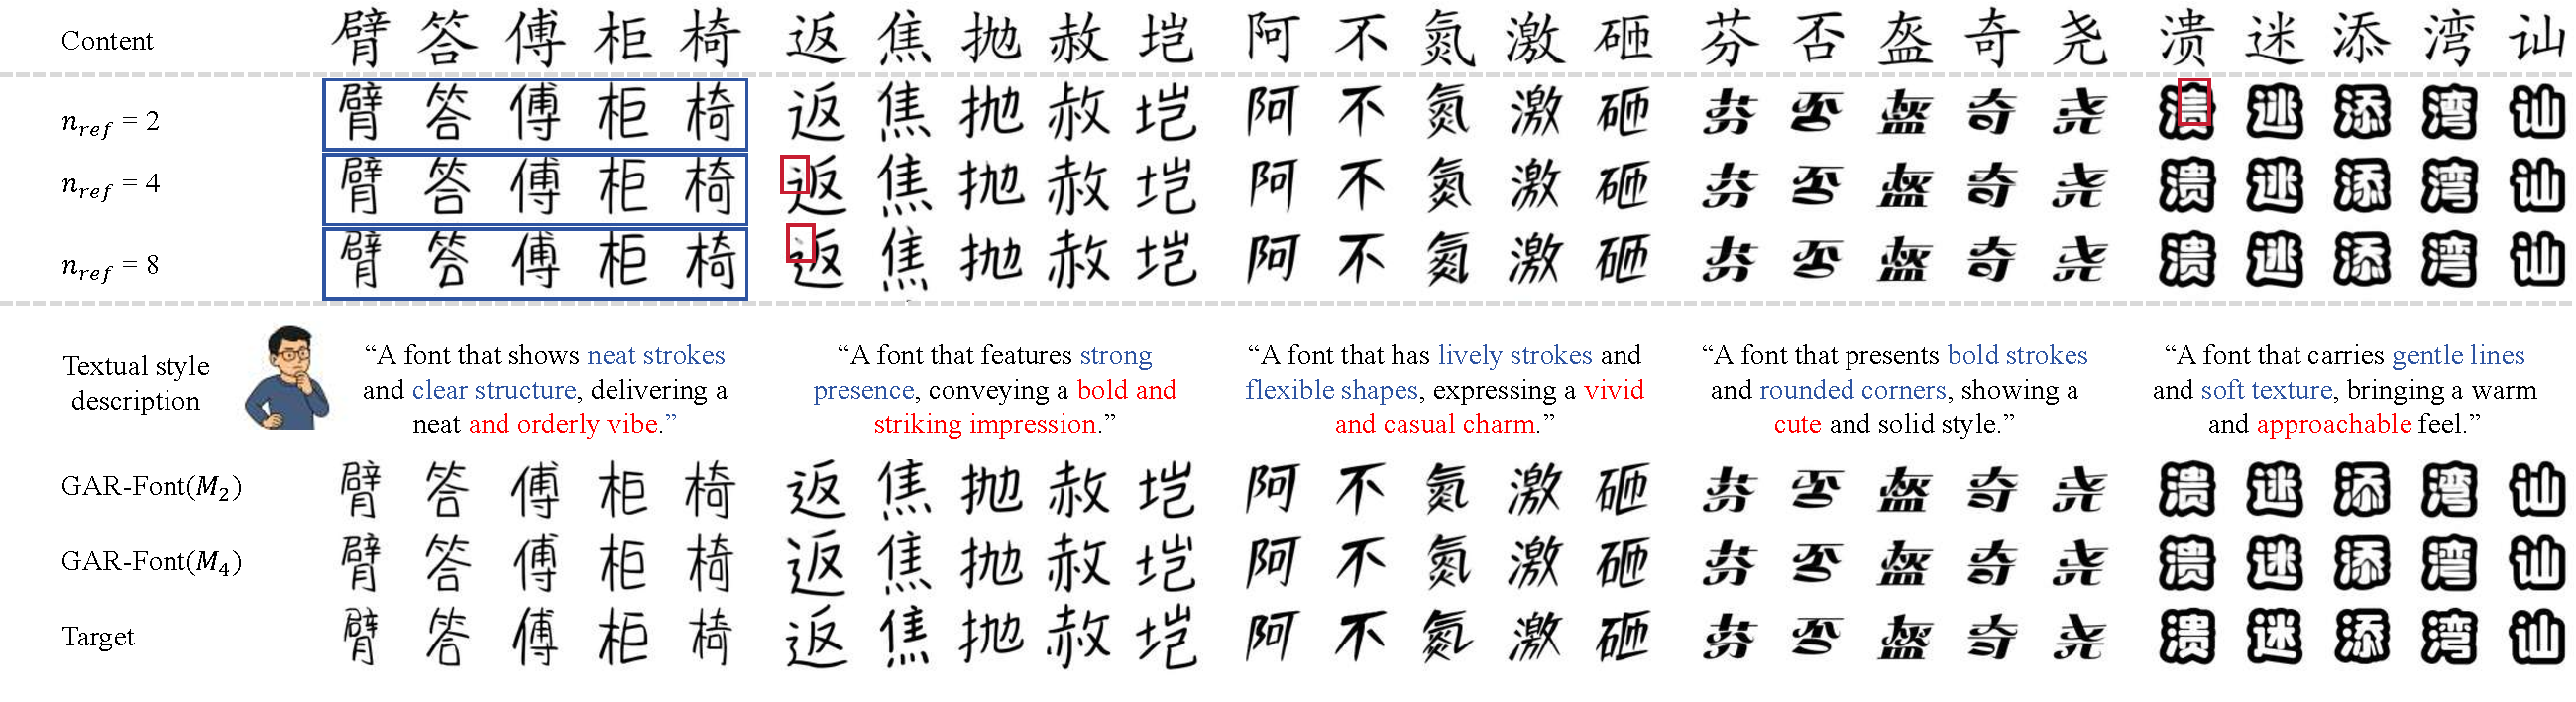
\includegraphics[width=\linewidth]{SUPP_IMGS/EX_Visualization/table2_supple_UFSC_Large_Post.pdf}
        \caption{\textit{UFSC}, Large dataset}
        \label{fig: supple_main2_ufsc_large_post}
    \end{subfigure}
    \\ % 强制换行
    \vspace{1mm}
    % -------- (b) Post --------
    \begin{subfigure}{0.92\linewidth}
        \centering
        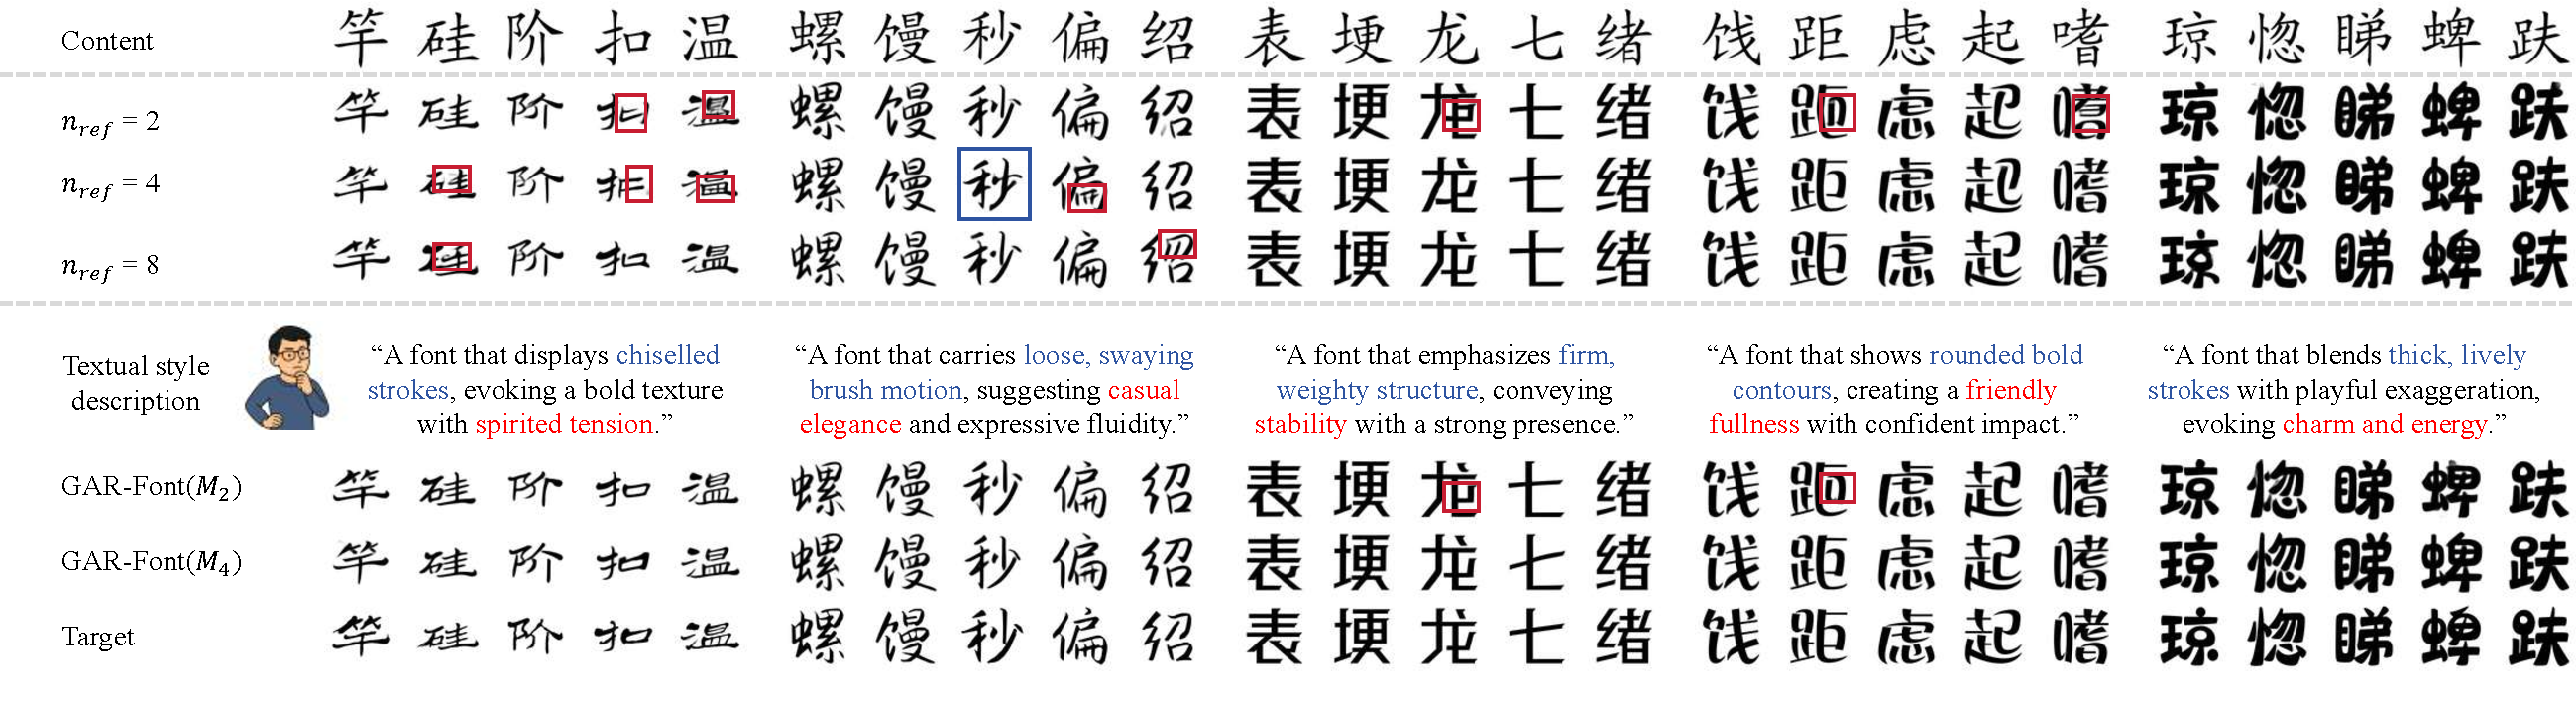
\includegraphics[width=\linewidth]{SUPP_IMGS/EX_Visualization/table2_supple_UFUC_Large_Post.pdf}
        \caption{\textit{UFUC}, Large dataset}
        \label{fig: supple_main2_ufuc_large_post}
    \end{subfigure}
    \vspace{-2mm}

    % -------- 第二组 Caption --------
    \caption{
        Qualitative results of Post-Refine multimodal FFG under \textit{UFSC} and \textit{UFUC} protocols
        (Large dataset). 
        \textcolor{ex2figure_red}{\fbox{\rule{0pt}{4pt}\rule{4pt}{0pt}}} denotes local slight structural mistakes, 
        and \textcolor{ex2figure_blue}{\fbox{\rule{0pt}{4pt}\rule{4pt}{0pt}}} marks stylistic drift.
    }
    \label{fig: supple_main2_large_post}

\end{figure*}




% \begin{figure*}[t]
%     \centering

%     % -------- (a) --------
%     \begin{subfigure}{0.95\linewidth}
%         \centering
%         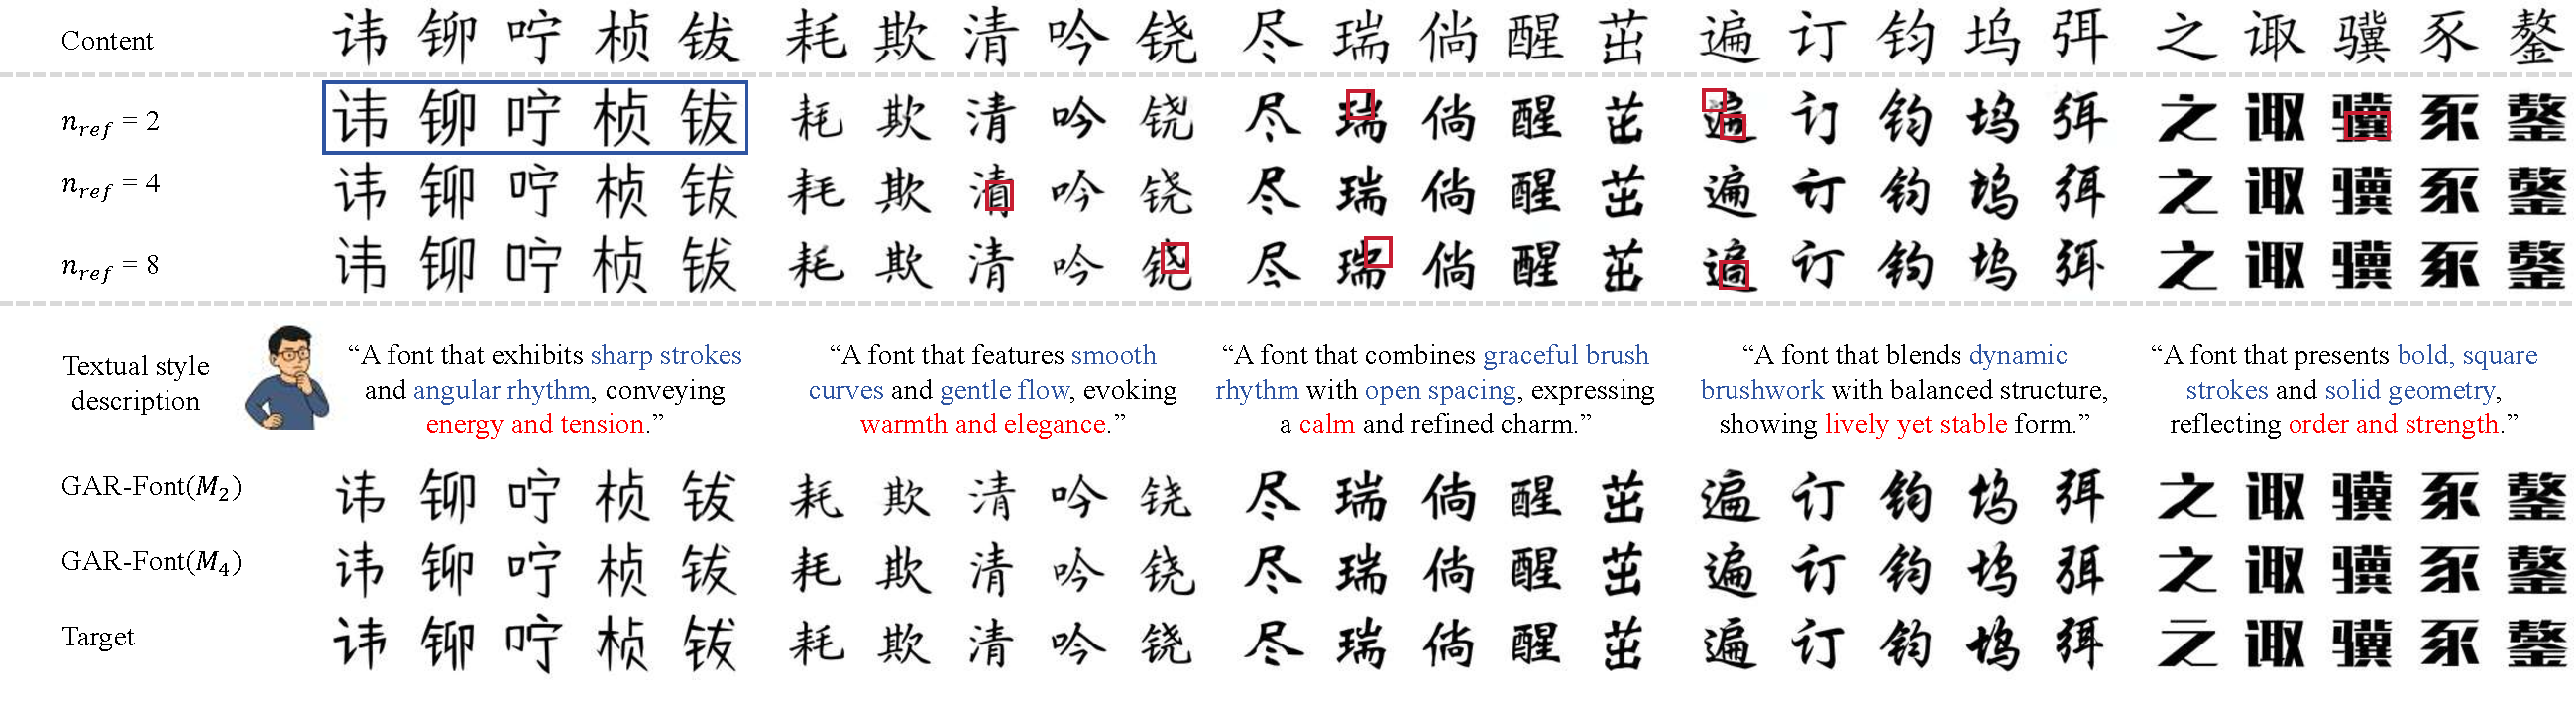
\includegraphics[width=\linewidth]{SUPP_IMGS/EX_Visualization/table2_supple_UFSC_Large_Pre.pdf}
%         \caption{UFSC, \textit{Large} dataset}
%         \label{fig: supple_main2_ufsc_large_pre}
%     \end{subfigure}

%     \vspace{2mm}

%     % -------- (b) --------
%     \begin{subfigure}{0.95\linewidth}
%         \centering
%         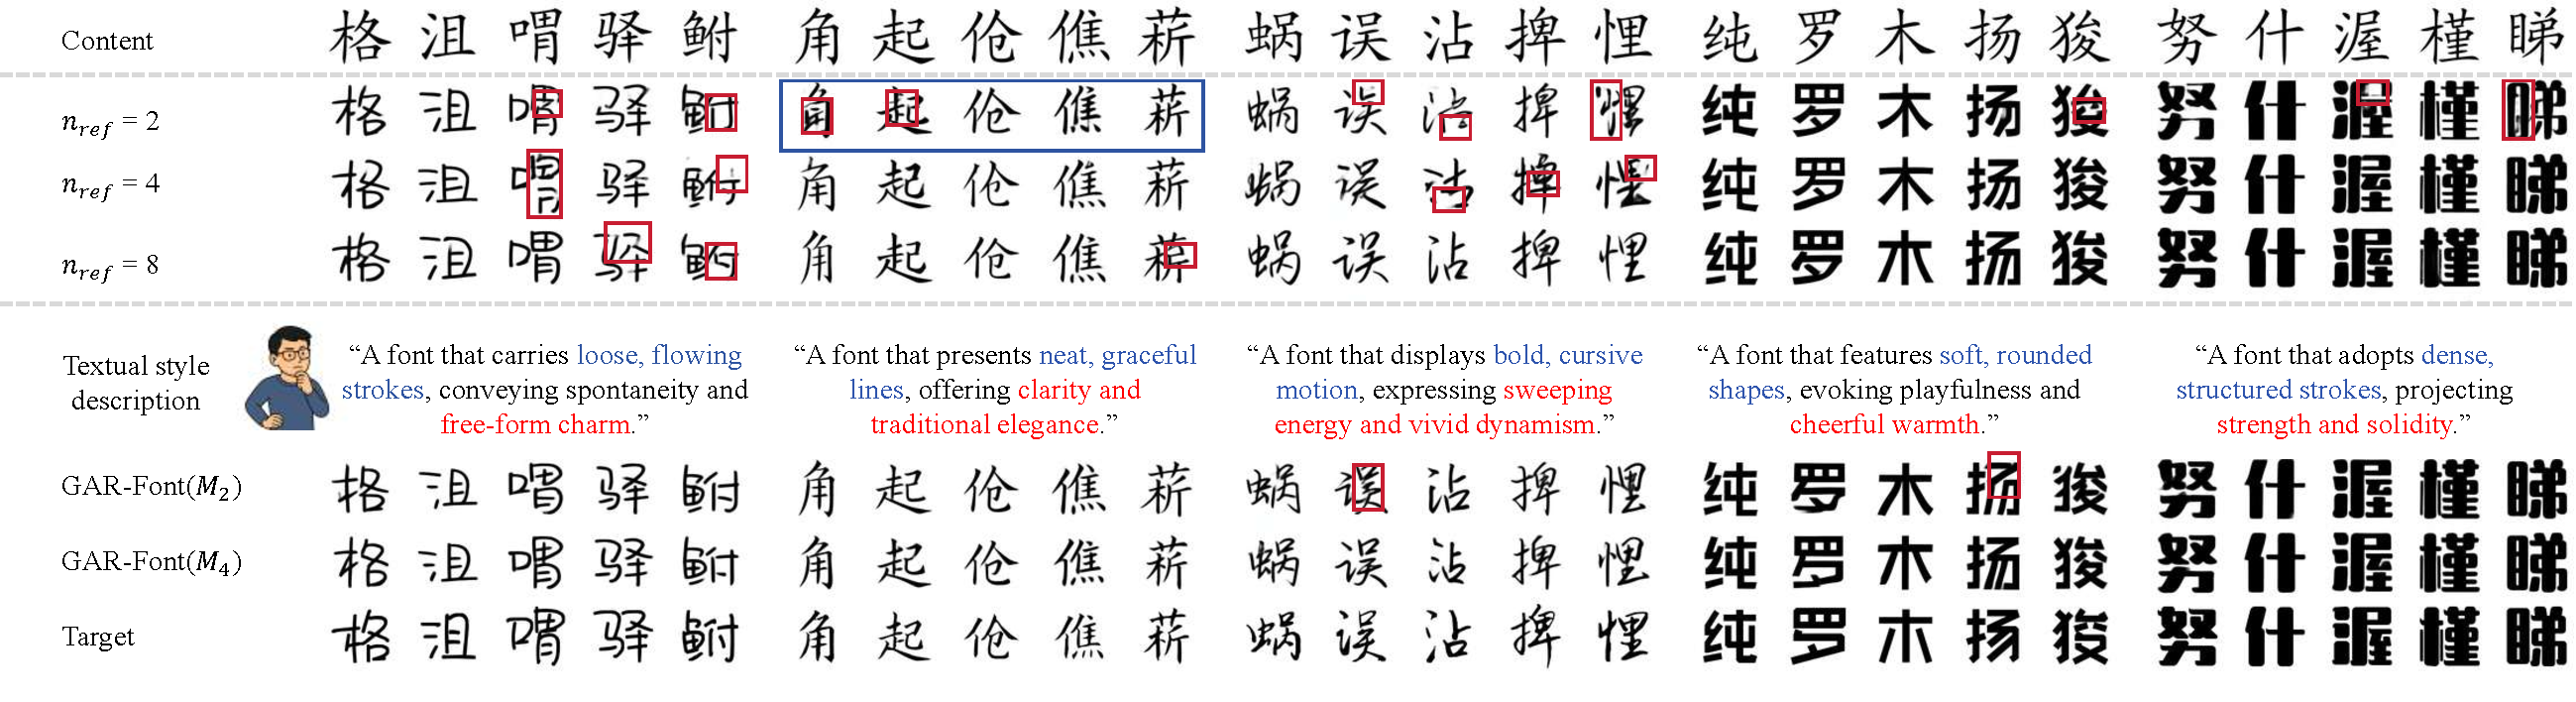
\includegraphics[width=\linewidth]{SUPP_IMGS/EX_Visualization/table2_supple_UFUC_Large_Pre.pdf}
%         \caption{UFUC, \textit{Large} dataset}
%         \label{fig: supple_main2_ufuc_large_pre}
%     \end{subfigure}

%     \vspace{2mm}

%     % -------- main caption --------
%     \caption{
%         Qualitative results on Pre-Train multimodal FFG under UFSC and UFUC protocols
%         (\textit{Large} dataset). 
%         \textcolor{ex2figure_red}{\fbox{\rule{0pt}{4pt}\rule{4pt}{0pt}}} denotes local slight structural mistakes,
%         and \textcolor{ex2figure_blue}{\fbox{\rule{0pt}{4pt}\rule{4pt}{0pt}}} marks samples with stylistic drift.
%     }
%     \label{fig: supple_main2_large_pre_all}
% \end{figure*}



% \begin{figure*}[t]
%     \centering

%     % -------- (a) --------
%     \begin{subfigure}{0.95\linewidth}
%         \centering
%         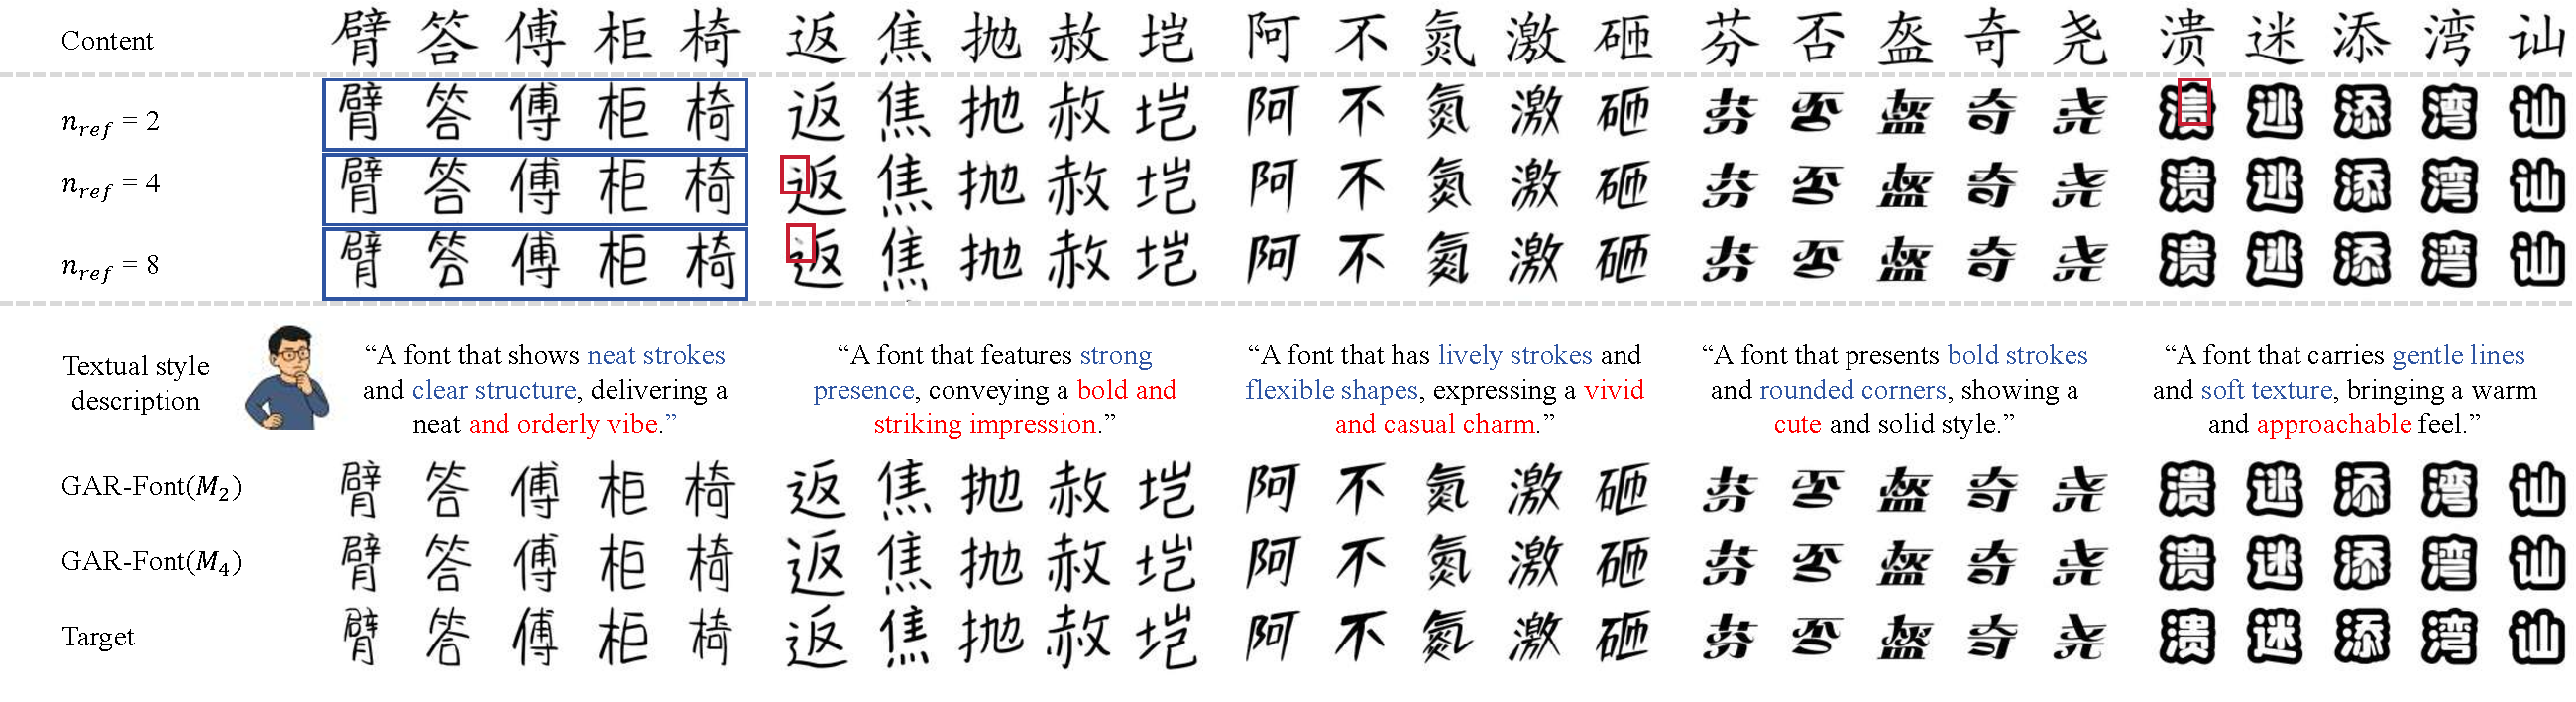
\includegraphics[width=\linewidth]{SUPP_IMGS/EX_Visualization/table2_supple_UFSC_Large_Post.pdf}
%         \caption{UFSC, \textit{Large} dataset}
%         \label{fig: supple_main2_ufsc_large_post}
%     \end{subfigure}

%     \vspace{2mm}

%     % -------- (b) --------
%     \begin{subfigure}{0.95\linewidth}
%         \centering
%         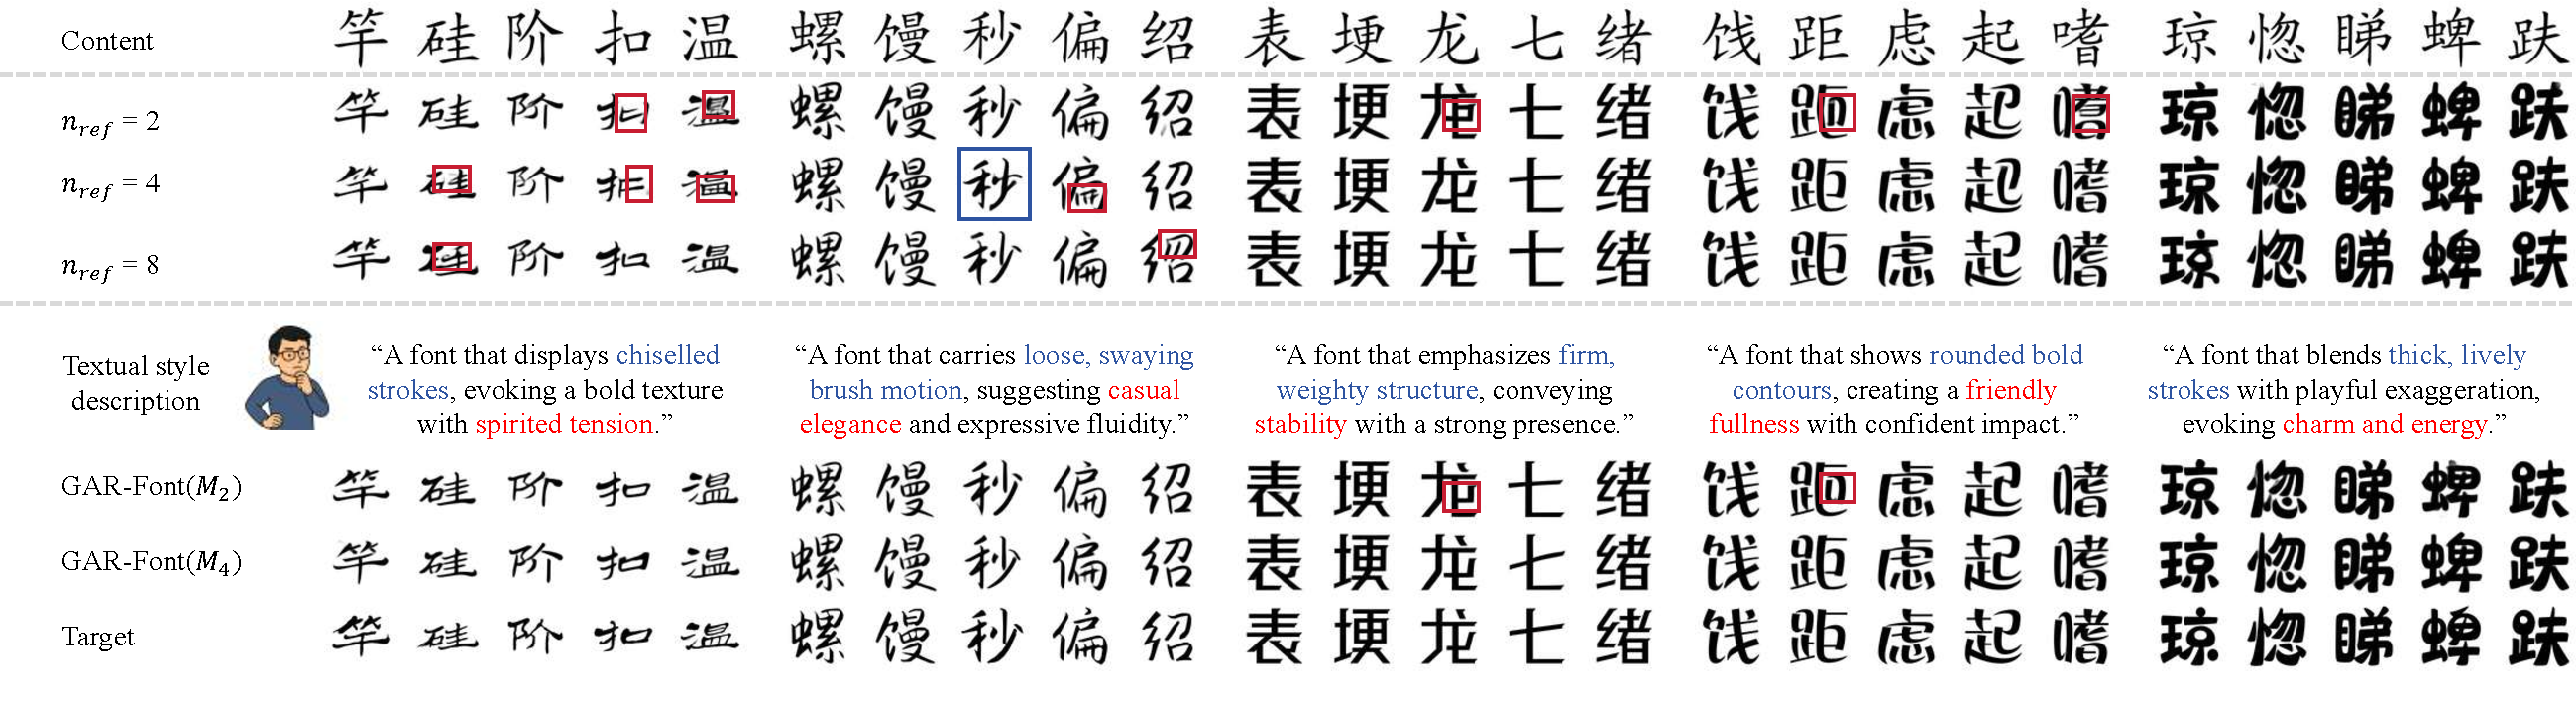
\includegraphics[width=\linewidth]{SUPP_IMGS/EX_Visualization/table2_supple_UFUC_Large_Post.pdf}
%         \caption{UFUC, \textit{Large} dataset}
%         \label{fig: supple_main2_ufuc_large_post}
%     \end{subfigure}

%     \vspace{2mm}

%     % -------- main caption --------
%     \caption{
%         Qualitative results of Post-Refine multimodal FFG under UFSC and UFUC protocols
%         (\textit{Large} dataset). 
%         \textcolor{ex2figure_red}{\fbox{\rule{0pt}{4pt}\rule{4pt}{0pt}}} denotes local slight structural mistakes, 
%         and \textcolor{ex2figure_blue}{\fbox{\rule{0pt}{4pt}\rule{4pt}{0pt}}} marks stylistic drift.
%     }
%     \label{fig: supple_main2_large_post}
% \end{figure*}
\begin{figure*}[t]
  \centering
  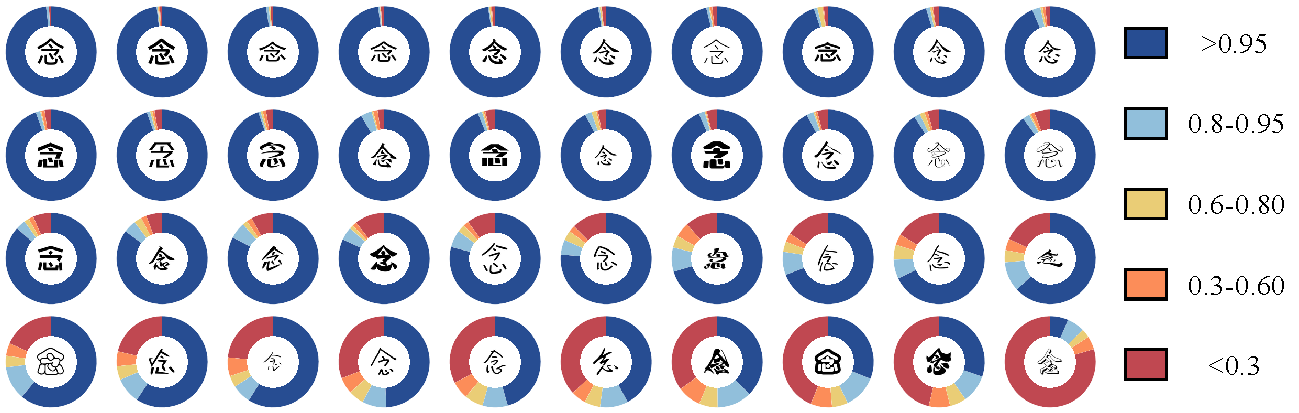
\includegraphics[width=0.95\linewidth]{SUPP_IMGS/Failure_Analysis/analysis_final.pdf}
  \vspace{-3mm}
  \caption{Content confidence distribution of GAR-Font generated characters across different font styles. Each pie chart corresponds to a specific font, indicated by the central character. The color segments represent the proportion of samples falling into different content confidence ranges, highlighting that more complex styles tend to have lower content confidence.}
  \vspace{-3mm}
  \label{fig:supple_analysis}
\end{figure*}



\begin{figure}[t]
  \centering
  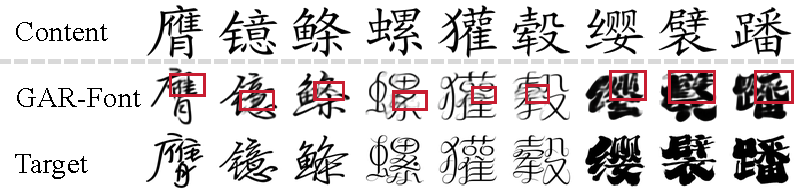
\includegraphics[width=0.95\linewidth]{SUPP_IMGS/Failure_Analysis/Failure_revised.pdf}
  \vspace{-3mm}
  \caption{Failure cases. \textcolor{ex2figure_red}{\fbox{\rule{0pt}{4pt}\rule{4pt}{0pt}}} highlights regions with dense details where GAR-Font tends to produce distorted strokes.}
  \vspace{-3mm}
  \label{fig:supple_failure_cases}
\end{figure}

\section{Visualization Results}
\label{sec:vis_results}
\subsection{Comparison on Few-shot Font Generation}
% UFSC， UFUC，  Large dataset
% UFSC,  UFUC,  Small dataset
We provide complete visualizations for the experiment in Section 5.1. In addition to the main results, Figure~\ref{fig: supple_main1_all} offer a granular analysis of our architectural decisions. 

In Figure~\ref{fig: supple_main1_all}, we show the full qualitative comparisons of visual-only FFG models trained on Small and Large datasets, evaluated under both \textit{UFSC} and \textit{UFUC} protocols. These results indicate that methods such as LF--Font, VQ-Font, DG-Font, CF-Font and Diff-Font often fail to preserve structural fidelity in intricate fonts. IF-Font tends to produce incomplete characters, while Font-Diffuser generates with inaccurate stroke widths. In contrast, GAR-Font($I_8$,+NFA+SE) achieves the best style fidelity while maintaining structural consistency, effectively capturing fine stroke details of the target fonts.


\subsection{Efficient Vision-Language Adaptation}

\subsubsection{Pretrain}
% UFSC， UFUC，  Large dataset

We provide full qualitative results complementing the experiment in Section~5.2. 
In Figure~\ref{fig: supple_main2_large_pre_all}, we show multimodal FFG comparisons under both \textit{UFSC} and \textit{UFUC} settings on the Large dataset, illustrating the improvements introduced by incorporating textual style descriptions in GAR-Font($M_2$) and GAR-Font($M_4$) compared with their vision-only counterparts. With textual style guidance, GAR-Font($M_2$) and GAR-Font($M_4$) better align with the target style, generating glyphs with strokes closely matching the target and improved structural fidelity.


\subsubsection{Post-Refinement}
% UFSC， UFUC，  Large dataset
To further assess the potential of our efficient vision–language adaptation, we apply the complete post-refinement pipeline (NFA and SE) to GAR-Font($M_2$) and GAR-Font($M_4$). 
Figure~\ref{fig: supple_main2_ufsc_large_post} presents qualitative results under \textit{UFSC} and \textit{UFUC} on the Large dataset. Applying NFA and SE post-refinement significantly improves both structural and style fidelity for all models. Textual guidance further enables GAR-Font($M_2$) and GAR-Font($M_4$) to more accurately capture the target style, yielding glyphs with improved style fidelity.

\subsection{More GAR-Font Generation Examples}
To illustrate the capabilities of GAR-Font, we generate the full GB2312 character set for five test fonts with GAR-Font($I_8$, +NFA+SE, trained on Large dataset) and randomly select 1,280 samples from each font. The generated glyphs are shown in Figures ~\ref{fig: add_sheet_1}-~\ref{fig: add_sheet_5} , demonstrating the model’s ability to produce large-scale character sets while faithfully preserving each font’s distinctive stylistic features.


\section{Failure Cases and Analysis}
\label{sec:Failure_cases}

While GAR-Font generally performs well, distortions and blurring occasionally appear in dense-stroke regions of highly complex fonts (\cref{fig:supple_failure_cases}). To investigate this, we applied a content classifier to all \textit{UFUC} samples generated by GAR-Font($I_8$,+NFA+SE), using the softmax output as a measure of content confidence. The results reveal a clear trend: content confidence notably decreases as stylistic complexity increases (\cref{fig:supple_analysis}), suggesting the model sometimes sacrifices structural accuracy to better capture stylistic features.

We hypothesize that this structural degradation results from the error accumulation inherent in autoregressive modeling. Without explicit structural constraints, the model tends to drift when generating intricate stroke patterns. A promising direction for future work is to incorporate explicit structural priors, such as character skeletons or stroke sequences, to guide the generation process. This would help preserve structural fidelity in complex styles.


\begin{figure*}
    \centering
    \includegraphics[width=0.95\linewidth]{SUPP_IMGS/Samples_Sheet/gen_soft_BigruixianBoldkGBV1.0_sample_12.png}
    \vspace{-3mm}
    \caption{Generated glyphs from test fonts using GAR-Font($I_8$, +NFA+SE, Large dataset).}
    \label{fig: add_sheet_1}
    \vspace{-3mm}
\end{figure*}
\clearpage
\begin{figure*}
    \centering
    \includegraphics[width=0.95\linewidth]{SUPP_IMGS/Samples_Sheet/gen_soft_FZBaiZhouRenZheTiS_sample_13.png}
    \vspace{-3mm}
    \caption{Generated glyphs from test fonts using GAR-Font($I_8$, +NFA+SE, Large dataset).}
    \label{fig: add_sheet_2}
    \vspace{-3mm}
\end{figure*}
\clearpage
\begin{figure*}
    \centering
    \includegraphics[width=0.95\linewidth]{SUPP_IMGS/Samples_Sheet/gen_soft_FZSJ-MINGYSJZ_sample_14.png}
    \vspace{-3mm}
    \caption{Generated glyphs from test fonts using GAR-Font($I_8$, +NFA+SE, Large dataset).}
    \label{fig: add_sheet_3}
    \vspace{-3mm}
\end{figure*}
\clearpage
\begin{figure*}
    \centering
    \includegraphics[width=0.95\linewidth]{SUPP_IMGS/Samples_Sheet/gen_soft_MiNiJianYouXian_sample_9.png}
    \vspace{-3mm}
    \caption{Generated glyphs from test fonts using GAR-Font($I_8$, +NFA+SE, Large dataset).}
    \label{fig: add_sheet_4}
    \vspace{-3mm}
\end{figure*}
\clearpage
\begin{figure*}
    \centering
    \includegraphics[width=0.95\linewidth]{SUPP_IMGS/Samples_Sheet/gen_soft_zihun40hao-xiaochengfeifanti-Regular_sample_9.png}
    \vspace{-3mm}
    \caption{Generated glyphs from test fonts using GAR-Font($I_8$, +NFA+SE, Large dataset).}
    \label{fig: add_sheet_5}
    \vspace{-3mm}
\end{figure*}
\clearpage

\end{document}
